\newcommand{\NWtarget}[2]{\hypertarget{#1}{#2}}
\newcommand{\NWlink}[2]{\hyperlink{#1}{#2}}
\newcommand{\NWtxtMacroDefBy}{Fragment defined by}
\newcommand{\NWtxtMacroRefIn}{Fragment referenced in}
\newcommand{\NWtxtMacroNoRef}{Fragment never referenced}
\newcommand{\NWtxtDefBy}{Defined by}
\newcommand{\NWtxtRefIn}{Referenced in}
\newcommand{\NWtxtNoRef}{Not referenced}
\newcommand{\NWtxtFileDefBy}{File defined by}
\newcommand{\NWtxtIdentsUsed}{Uses:}
\newcommand{\NWtxtIdentsNotUsed}{Never used}
\newcommand{\NWtxtIdentsDefed}{Defines:}
\newcommand{\NWsep}{${\diamond}$}
\newcommand{\NWnotglobal}{(not defined globally)}
\newcommand{\NWuseHyperlinks}{}
% -*- mode: latex; coding: utf-8 -*-

\documentclass[%
    a4paper,    % Use A4, not US letter!
    justified,  % Use justified text
    nobib,      % Disable natbib
    openany     % Remove blank pages used for two page layout
]{tufte-book}

% -*- mode: latex; coding: utf-8 -*-

\makeatletter
% textwidth Tuftian float for listings
\newenvironment{listing}[1][htbp]
  {\ifvmode\else\unskip\fi\begin{@tufte@float}[#1]{lstlisting}{}}
  {\end{@tufte@float}}
% fullwidth Tuftian float for listings
\newenvironment{listing*}[1][htbp]%
  {\ifvmode\else\unskip\fi\begin{@tufte@float}[#1]{lstlisting}{star}}
  {\end{@tufte@float}}
% enable re-use of \listoflistings facility
\def\ext@lstlisting{lol}
% show listing number in caption even though \lst@@caption is empty
\def\fnum@lstlisting{\lstlistingname~\thelstlisting}
\makeatother

\renewcommand{\label}[1]{\@tufte@label{##1}}%
% Handle subfigure package compatibility
\ifthenelse{\boolean{@tufte@packages@subfigure}}{%
  % don't move the label while inside a \subfigure or \subtable command
  \global\let\label\@tufte@orig@label%
}{}% subfigure package is not loaded

\makeatletter
\setboolean{@tufte@packages@subfigure}{true}
\makeatother

% Load packages
% ---------------------------------------------------------------------------
\usepackage[usenames,dvipsnames,svgnames]{xcolor}
\usepackage{minted}
\usepackage[english]{babel}              % English hyphenation
\usepackage[utf8]{inputenc}              % UTF-8 input encoding
% \usepackage[T1]{fontenc}                 % hyphenation of words with ä,ö and ü
\usepackage{booktabs,tabularx}           % package for nicer tables
\usepackage{pgfgantt}                    % Provides GANTT charts
\usepackage[owncaptions]{vhistory}       % Provides framework for creating history outline
\usepackage{csquotes}                    % Quotes
\usepackage{nameref}                     % Allows referencing of names
\usepackage{blindtext}                   % Dummy text
\usepackage[pages=some]{background}            % Backgrounds
\usepackage[absolute,overlay]{textpos}
\usepackage{hyperref}
\usepackage{makeidx}
\usepackage[nonumberlist,nomain]{glossaries}
\usepackage{todonotes}
\usepackage[
    backend=biber,
    style=ieee,
    sortlocale=de_DE,
    natbib=true,
    url=false, 
    doi=true,
    eprint=false
]{biblatex}
\usepackage{bookmark}
\usepackage{esvect}                          % Provides nicer vector display in math mode
\usepackage[inline]{enumitem}
\usepackage{tikz}
\usepackage{float}
\usepackage{cleveref}

% Settings
%---------------------------------------------------------------------------
% TIKZ: A lot of arrows for TIKZ
\usetikzlibrary{arrows.meta}

% TUFTE: Do not break when there already is a break
% Source: https://tex.stackexchange.com/questions/291746/tufte-latex-newthought-after-section
\makeatletter
\def\tuftebreak{%
  \if@nobreak\else
    \par
    \ifdim\lastskip<\tufteskipamount
      \removelastskip \penalty -100
      \tufteskip
    \fi
  \fi
}
\makeatother

% Environments
% ---------------------------------------------------------------------------
\newenvironment{loggentry}[2]% date, heading
{\noindent\textbf{#1}\marginnote{#2}\\}

% Commands
%---------------------------------------------------------------------------
% -*- mode: latex; coding: utf-8 -*-

% Prints the month name (e.g., January) and the year (e.g., 2008)
\newcommand{\monthyear}{%
  \ifcase\month\or January\or February\or March\or April\or May\or June\or
  July\or August\or September\or October\or November\or
  December\fi\space\number\year
}

% Provide references to footnotes to re-use existing.
\newcommand{\footref}[1]{\textsuperscript{\ref{#1}}}

% Used for tables
\newcommand{\ra}[1]{\renewcommand{\arraystretch}{#1}}

% Provide possibility to cite also the first name of an author
% https://tex.stackexchange.com/questions/211755/controlling-first-name-display-in-biblatex-citeauthor
\DeclareCiteCommand{\citeauthorfin}
  {\renewcommand*{\mkbibnamelast}[1]{####1}%
   \boolfalse{citetracker}%
   \boolfalse{pagetracker}%
   \usebibmacro{prenote}}
  {\ifciteindex
     {\indexnames{labelname}}
     {}%
   % \printnames[initsonly]{author} % too strong, all is initials (D.E.K.)
   %\printnames[firstinits=true,first-last]{author}} % cannot:
   % \ExecuteBibliographyOptions{firstinits=false} % only in preamble!
   % so must use setkeys:
   \setkeys{blx@opt@pre}{firstinits=true}%
   \printnames[first-last]{author}%
   \setkeys{blx@opt@pre}{firstinits=false}% restore - assuming false is default, which here it is
  }
  {\multicitedelim}
  {\usebibmacro{postnote}}
\makeatother%
\DeclareCiteCommand{\citeauthorffn}
  {\renewcommand*{\mkbibnamelast}[1]{####1}%
   \boolfalse{citetracker}%
   \boolfalse{pagetracker}%
   \usebibmacro{prenote}}
  {\ifciteindex
     {\indexnames{labelname}}
     {}%
   \printnames[first-last]{author}}
  {\multicitedelim}
  {\usebibmacro{postnote}}

% Multiple footnotes
% https://tex.stackexchange.com/questions/28465/multiple-footnotes-at-one-point
\let\oldFootnote\footnote
\newcommand\nextToken\relax
\renewcommand\footnote[1]{%
    \oldFootnote{#1}\futurelet\nextToken\isFootnote}
\newcommand\isFootnote{%
    \ifx\footnote\nextToken\textsuperscript{,}\fi}
% Definition of colors
%---------------------------------------------------------------------------
% -*- mode: latex; coding: utf-8 -*-

\definecolor{linkblue}{rgb}{0,0,0.8}       % Standard
\definecolor{darkblue}{rgb}{0,0.08,0.45}   % Dark blue
\definecolor{bfhgrey}{rgb}{0.41,0.49,0.57} % BFH grey
\definecolor{linkcolor}{rgb}{0,0,0}
\colorlet{Black}{black}
\definecolor{keywords}{rgb}{255,0,0}
\definecolor{red}{rgb}{0.6,0,0}
\definecolor{green}{rgb}{0,0.5,0}
\definecolor{blue}{rgb}{0,0,0.5}
% Syntax colors
\definecolor{syntaxRed}{rgb}{0.6,0,0}
\definecolor{syntaxBlue}{rgb}{0,0,0.5}
\definecolor{syntaxComment}{rgb}{0,0.5,0}
% Background colors
\definecolor{titlepagecolor}{cmyk}{1,.60,0,.40}
\definecolor{syntaxBackground}{rgb}{0.95, 0.95, 0.95}

% (Code-) Listings
%---------------------------------------------------------------------------
% -*- mode: latex; coding: utf-8 -*-

\newminted{python}{%
    bgcolor=LightGray,
    escapeinside=||,
    linenos=true,
    mathescape=true,
}

% Generate index
%---------------------------------------------------------------------------
\makeindex

% Global variables
%---------------------------------------------------------------------------
\newcommand{\titletext}{QDE.}
\newcommand{\subtitletext}{A system for composing real time computer graphics.}
\newcommand{\subsubtitletext}{MTE7103 --- Master thesis}
\author[Sven Osterwalder]{Sven Osterwalder}
\publisher{Berne University of Applied Sciences}

% Commands
%----------------------------------------------------------------------------
\renewcommand\labelenumi{(\theenumi)}

% Background set up
%---------------------------------------------------------------------------
\backgroundsetup{
    scale=1,
    angle=0,
    opacity=1,
    contents={
        \begin{tikzpicture}[remember picture,overlay]
            \node[anchor=south west, inner sep=0pt,outer sep=0pt] at (current page.south west) {%
                
\includegraphics[width=1.0\paperwidth,height=0.5\paperheight]{images/bg}
            };
        \end{tikzpicture}
    }
}
\makeatletter
\def\printauthor{%
    {\large \@author}}
\makeatother

% Set up bibliography
%----------------------------------------------------------------------------
\addbibresource{inc/bibliography.bib}
\DefineBibliographyStrings{ngerman}{
    andothers = {{et\,al\adddot}},
}

\begin{document}

% Title Page and Abstract
%---------------------------------------------------------------------------
\setcounter{page}{1}
% -*- mode: latex; coding: utf-8 -*-

\begin{titlepage}
    \BgThispage
    \begin{fullwidth}%
        \sffamily%
        \fontsize{36}{40}\selectfont\par\noindent\textcolor{darkgray}{\allcaps{\titletext{}}}
        \vspace{3mm}
        \fontsize{18}{20}\selectfont\par\noindent\textcolor{darkgray}{\allcaps{\subtitletext{}}}
        \vspace{6mm}
        \fontsize{14}{16}\selectfont\par\noindent\allcaps{\subsubtitletext{}}%
        \vspace{24mm}
        \normalsize\normalfont%
        \begin{tabbing}
        xxxxxxxxxxxxxxx \= xxxxxxxxxxxxxxxxxxxxxxxxxxxxxxxxxxxxxxxxxxxxxxx \kill
        Major:          \> Computer science                              \\
        Author:         \> Sven Osterwalder\protect\footnotemark[1]{}    \\
        Advisor:        \> Prof.~Claude Fuhrer\protect\footnotemark[2]{} \\
        Expert:         \> Dr.~Eric Dubuis\protect\footnotemark[3]{}     \\
        Date:           \> \vhCurrentDate{}                              \\
        Version:        \> \vhCurrentVersion                             \\
        \end{tabbing}
        \vspace{10mm}
        \begin{tabularx}{0.5\textwidth}{@{}XX@{}}
            
\includegraphics[width=50px]{images/by-sa-big} & 
            
\includegraphics[height=20pt]{images/BFH_Logo_B} \\

            \tiny{\sffamily{This work is licensed under
            a~\href{http://creativecommons.org/licenses/by-sa/4.0/}{Creative
            Commons Attribution-ShareAlike 4.0 International
            License}.}}\index{license}
            & \tiny{\sffamily{Berne University of Applied Sciences}}\\
        \end{tabularx}
        \footnotetext[1][-10pt]{sven.osterwalder@students.bfh.ch}
        \footnotetext[2]{claude.fuhrer@bfh.ch}
        \footnotetext[3]{eric.dubuis@comet.ch}
    \end{fullwidth}%
\end{titlepage}
\restoregeometry
\thispagestyle{empty}%
\clearpage%
% -*- coding: utf-8 -*-

\chapter*{Abstract}
\label{chap:abstract}

\todo[inline]{Provide correct abstract.}
A highly optimized rendering algorithm based on ray
tracing is presented. It outperforms the classical ray tracing methods and
allows the rendering of ray traced scenes in real-time on the GPU.~The
classical approach for modelling scenes using triangulated meshes is replaced
by mathematical descriptions based on signed distance functions. The
effectiveness of the algorithm is demonstrated using a prototype application
which renders a simple scene in real-time.

% Richtet sich der Bericht an eine breitere Öffentlichkeit oder an technische Laien, die aufgrund fehlender
% Sachkenntnis nicht den ganzen Bericht lesen wollen, dann kann die Zusammenfassung zum
% wichtigsten Teil eines Berichts werden [3, p. 24]. Die Zusammenfassung ist der meistgelesene Teil
% einer Publikation. Sie gibt einen Überblick zur Problemstellung, zum Inhalt und zu den Resultaten des
% Berichts. Eine gute Zusammenfassung kann die Leserin, den Leser ermutigen, ausgewählte Teile der
% Arbeit oder den gesamten Bericht zu studieren.
% Die Zusammenfassung muss unabhängig vom Rest der Arbeit verständlich sein und besonders
% schlüssig formuliert werden. Literaturangaben werden in der Zusammenfassung keine gemacht.
% Die Zusammenfassung gehört an den Anfang eines Berichts. Oft wird sie auch mit Abstract oder
% Summary bezeichnet.
% Je nach Länge der Arbeit werden der Auftrag, die Ausgangslage, das Vorgehen und die wesentlichen
% Ergebnisse und Schlussfolgerungen des Berichts im Umfang zwischen einer halben und maximal einer
% ganzen A4-Seite dargelegt. Die eigenen Resultate bilden den inhaltlichen Schwerpunkt der
% Zusammenfassung.
% Die Zusammenfassung wird erst am Ende des Arbeitsprozesses verfasst.

% Table of contents / Lists of
%---------------------------------------------------------------------------
\tableofcontents{}
\listoffigures{}
\listoftables{}

% Main part
%---------------------------------------------------------------------------
\newpage{}
% -*- mode: latex; coding: utf-8 -*-

\chapter{Introduction}
\label{chap:introduction}

% Die Einleitung gibt Antwort auf die Frage, weshalb es den Bericht gibt und wie
% er zustande gekommen ist [3, p. 25]. Im ersten Teil wird das Thema der Arbeit
% eingeführt. Die Relevanz und Aktualität des Themas oder der fachliche Kontext
% der Untersuchung werden dazu kurz umschrieben. Die Einleitung hält explizit
% fest, welchen Auftrag der Bericht erfüllt [3, p. 25]. Der Auftrag muss so klar
% und präzise wie möglich formuliert werden. Auftraggeber und Auftragnehmer werden
% festgehalten. Der zweite Teil der Einleitung stellt den Ist-Zustand oder den
% bisherigen Wissensstand knapp dar. Darauf aufbauend wird das eigene Thema
% eingegrenzt. Es gibt Untersuchungen, bei denen es für das Verständnis wichtig
% ist, den genauen Ist-Zustand zu kennen. Wenn es für ein Projekt bereits ein
% Vorprojekt gibt, auf dessen Resultate der Bericht aufbaut, oder in Bauprojekten
% ist es üblich, die Ausgangslage in einem gesonderten Kapitel zu beschreiben. Im
% dritten Teil wird die präzise Fragestellung formuliert. Das Ziel des Berichts
% wird genannt und es wird erläutert, welchen Nutzen die Untersuchung haben soll.

\newthought{The application area of computer graphics} exists since the
beginning of modern computing. Computer scientists have always strived to create
realistic depictions of the observable reality.

\newthought{Over time various approaches} for creating artificial images (the so
called rendering) have evolved. One of these approaches is ray tracing. This was
introduced in~\citeyear{appel_techniques_1968}
by~\citeauthorfin{appel_techniques_1968} in the
article~\citetitle{appel_techniques_1968}~\cite{appel_techniques_1968}. In
\citeyear{whitted_improved_1980} this methods were improved
by~\citeauthorfin{whitted_improved_1980} in his work
\citetitle{whitted_improved_1980}~\cite{whitted_improved_1980}.

\newthought{Ray tracing captivates} through simplicity while providing a very
high image quality, including perfect refractions and reflections of light. For
a long time although, the approach was not efficient enough to deliver images in
real time, which requires creating at least 25 rendered images (frames) per
second. Otherwise, due to the human anatomy, the output is perceived as either
still and jerky images or as a too slow animation.

\newthought{Sphere tracing} is a ray tracing approach introduced
in~\citeyear{hart_sphere_1994} by~\citeauthorfin{hart_sphere_1994} in his
work~\citetitle{hart_sphere_1994}~\cite{hart_sphere_1994}. This approach is
faster than the classical ray tracing approaches in its method of finding
intersections between rays and objects.

\newthought{Graphics processing units (GPUs)} have evolved over time and have
become exponentially more powerful in processing power. Since around 2009, GPUs are able to
produce real time computer graphics using sphere tracing. While allowing ray
tracing in real time on modern GPUs, sphere tracing has, however, a clear
disadvantage. The de facto way of representing the surface of objects using triangle based
meshes cannot be used directly. Instead, distance functions are used for
modeling the surfaces as seen from any view point.

\section{Purpose and conditions}
\label{sec:purpose}

\subsection{Motivation}
\label{subsec:motivation}

\newthought{Up to this point in time} there are no solutions (at least none are
known to the author) that provide a convenient way for modeling, animating and
rendering objects and scenes using signed distance functions for modeling and
sphere tracing for rendering.
Most of the solutions using sphere tracing implement it by having one or
multiple big fragment shaders containing everything from modeling to lighting.
Other solutions provide node based approaches, but they allow either no sphere
tracing at all, meaning they use rasterization, or they provide nodes containing
(fragment-) shader code, which leads again to a single big fragment shader.

\newthought{This thesis} aims at designing and developing a program which
provides both, a node based approach for modeling and animating objects using
signed distance functions and allowing the rendering of scenes using sphere
tracing, efficiently enough to be executed in real time on the GPU.

\subsection{Objectives and limitations}
\label{subsec:objectives}

\newthought{The objective of this thesis} is the design and development of a
program for \textit{modeling}, \textit{composing} and \textit{rendering} real
time computer graphics by providing a graphical toolbox.

\newthought{Modeling} is done by composing simple objects into complex objects
and scenes using a node based graph structure of~\enquote{nodes}.

\newthought{Composing} includes two aspects: the combination of objects into
scenes, and the creation of an animation which is defined by multiple scenes
which follow a chronological order. The first aspect is realized by a scene
graph structure. The second aspect is realized by a time line.

\newthought{For rendering}, a highly optimized algorithm based on ray tracing is
used. The algorithm is called sphere tracing and allows the rendering of ray
traced scenes in real time on the GPU. Contingent upon the rendering algorithm
used all objects are modeled using distance functions.

\newthought{Required objectives} are the following:
\begin{itemize}
  \item Development of an editor for creating and editing real time rendered
    scenes, containing the following features.
    \begin{itemize}
      \item A scene tree, allowing management (creation and deletion) of
        scenes.
      \item One node-based graph structure for each scene in the scene tree.
        This allows the composition of scenes using
        nodes and connections between the nodes.
    \item Nodes
      \begin{itemize}
        \item Simple objects defined by signed distance functions: In this
          thesis the objects are limited to cube and sphere (other solids could
          be modeled in the same way).
        \item Simple operations: Union, Intersection, Subtraction.
        \item Transformations: Rotate, Translate and Scale.
        \item Camera.
        \item Renderer (ray traced rendering using sphere tracing)
        \item Point light sources.
      \end{itemize}
    \end{itemize}
\end{itemize}

\section{Related works}
\label{sec:related-works}

\newthought{Preliminary} to this thesis two project works were completed.
The first was \enquote{Volume ray casting --- basics \&
principles}~\cite{osterwalder-volume-2016}, which describes the concepts
of sphere tracing The second was \enquote{QDE
--- a visual animation system, architecture}~\cite{osterwalder-qde-2016}, which
established the concepts of an editor and a player component, as well as
the basis for a possible software architecture for these components.

\newthought{For clarity in the explanation} of this thesis first the
architecture is presented, see section~\enquote{\nameref{soarch}}. Then the rendering is
presented in section~\enquote{\nameref{sec:rendering}}.

\section{Document structure}
\label{sec:document-structure}

\newthought{This document is divided into six chapters}, the first being this
chapter,~\enquote{\nameref{chap:introduction}}. The second
chapter~\enquote{\nameref{chap:administrative-aspects}} shows the planning of
the project, including the persons involved, the deliverables, and phases and
milestones.

\newthought{The administrative aspects are followed by} the
chapter~\enquote{\nameref{fundamentals}}. The purpose of this chapter is to
present the principles, based on the previous project works mentioned above that
this thesis is built upon.

\newthought{The next chapter} on~\enquote{\nameref{chap:methodologies}}
introduces a concept called literate programming and elaborates some details of
the implementation using this. Additionally it introduces standards and
principles for implementation of the developed software.

\newthought{The following chapter} on~\enquote{\nameref{chap:implementation}}
describes the editor component.
% TODO: Elaborate more? OK like this.

\newthought{The last chapter}~\enquote{\nameref{chap:discussion-conclusion}}
considers the methodologies as well as the results. Some further work on the
editor and the player components is proposed as well.

\newthought{After the regular content} follow appendices,
see~\enquote{\nameref{part:appendix}}, detailing the requirements for building the
above-mentioned components, and the actual source code in form of a literal
program.

% TODO: Add missing content, if content _is_ missing.
% -*- mode: latex; coding: utf-8 -*-

\chapter{Administrative aspects}
\label{chap:administrative_aspects}

% Link to previous
% Make a connection to what has immediately gone before. Recap the last chapter.
% In the last chapter I showed that… Having argued in the previous chapter that…
% As a result of x, which I established in the last chapter….. It is also possible
% to make a link between this chapter and the whole argument… The first step in
% answering my research question (repeat question) .. was to.. . In the last
% chapter I …
\newthought{The previous chapter} provided an introduction to this thesis by
outlining the purpose and conditions, the previous works and structure of this
work.

% Focus: What does this chapter specifically do?
% Now focus the reader’s attention on what this chapter is specifically going to
% do and why it is important. In this chapter I will examine.. I will present… I
% will report … This is crucial in (aim of thesis/research question) in order to….
\newthought{This chapter} covers administrative aspects of this project,
although they are not required for an understanding of the results.

% Overview: How is it done?
% The third paragraph simply outlines the way that you are going to achieve the
% aim spelled out in the previous paragraph. It’s really just a statement of the
% contents in the order that the reader will encounter them. It is important to
% state these not simply as topics, but actually how they build up the internal
% chapter argument… I will begin by examining the definitions of, then move to
% seeing how these were applied… I first of all explain my orientation to the
% research process, positioning myself as a critical scholar.. I then explain the
% methodology that I used in the research, arguing that ethnography was the most
% suitable approach to provide answers to the question of…
\newthought{The first section} defines the persons involved and their roles
during this thesis. Afterwards the deliverable items are defined and described.
The last section elaborates on the organization of the project work involved,
including meetings, phases and milestones as well as the work schedule.

\section{Involved persons}
\label{sec:involved_persons}

\begin{table}[h]
  \caption{List of the involved persons.}
  \begin{tabularx}{\textwidth}{llX}
    \toprule
    \textbf{Role} & \textbf{Name} & \textbf{Task} \\
    \midrule
    \textit{Author}  & Sven Osterwalder\protect\footnotemark[1]{} & Author of the thesis.\\
    \textit{Advisor} & Prof.\ Claude Fuhrer\protect\footnotemark[2]{} & Supervises the student doing the thesis.\\
    \textit{Expert}  & Dr.\ Eric Dubuis\protect\footnotemark[3]{}     & Provides expertise concerning the thesis's subject, monitors and grades the thesis.\\
    \bottomrule
  \end{tabularx}
\end{table}
\footnotetext[1]{sven.osterwaldertudents.bfh.ch}
\footnotetext[2]{claude.fuhrer@bfh.ch}
\footnotetext[3]{eric.dubuis@comet.ch}

\newpage{}

\section{Deliverables}
\label{sec:deliverables}

\begin{table}[h]
  \caption{List of deliverables.}
  \begin{tabularx}{\textwidth}{lX}
    \toprule
    \textbf{Deliverable} & \textbf{Description} \\
    \midrule
    \textit{Report} & The report contains the theoretical and technical details for
    implementing a system for composing real time computer graphics. \\
    \midrule
    \textit{Implementation} & The implementation of the system for composing real time
    computer graphics, developed during this project. \\
    \bottomrule
  \end{tabularx}
\end{table}

\section{Organization of work}
\label{sec:organization-of-work}

\subsection{Meetings}
\label{subsec:meetings}

\newthought{Various meetings} with the supervisor and the expert helped to reach
the defined goals and to prevent erroneous directions during the project. The
supervisor and the expert supported the author by providing suggestions
throughout the work period. The minutes of some meetings may be
found under the appendix meeting minutes.~\todo{Add correct reference}

\subsection{Phases and milestones}
\label{subsec:project-phases-milestones}

\begin{table}[h]
  \caption{Phases of the project.}
  \begin{tabularx}{\textwidth}{Xr}
    \toprule
    \textbf{Phase}   & \textbf{Week / 2017} \\
    \midrule
    Start of the project & 8 \\
    Definition of objectives and constraints & 8-9 \\
    Documentation and development & 8-30 \\
    Final review & 30-31 \\
    Preparation for the defense of the thesis & 31-32 \\
    \bottomrule
  \end{tabularx}
\end{table}

\begin{table}[h]
  \caption{Milestones of the project.}
  \begin{tabularx}{\textwidth}{Xr}
    \toprule
    \textbf{Milestone}   & \textbf{End of week / 2017} \\
    \midrule
    Project structure is set up & 8 \\
    Mandatory project goals are reached & 30 \\
    Hand-in of the thesis & 31 \\
    Defense of the thesis & 32 \\
    \bottomrule
  \end{tabularx}
\end{table}

\newpage{}

\subsection{Schedule}
\label{subsec:project-schedule}

\begin{figure*}[ht]
    \begin{ganttchart}[
        vgrid,
        x unit=4.5mm,
        y unit chart=0.87cm,
        bar/.append style={fill=bfhgrey!50},
    ]{1}{26}
        \gantttitle{2017}{26} \ganttnewline{}
        \gantttitlelist{7,...,32}{1} \ganttnewline{}
        \ganttbar{Start of the project}{1}{1} \ganttnewline{}
        \ganttmilestone{Project is set up}{1} \ganttnewline{}
        \ganttlinkedbar{Objectives and limitations}{2}{3} \ganttnewline{}
        \ganttlinkedbar{Documentation}{3}{23} \ganttnewline{}
        \ganttbar{Development}{3}{23} \ganttnewline{}
        \ganttmilestone{Goals reached}{23} \ganttnewline{}
        \ganttlinkedbar{Corrections}{23}{24} \ganttnewline{}
        \ganttmilestone{Hand-in}{24} \ganttnewline{}
        \ganttlinkedbar{Thesis' defense preparation}{25}{26} \ganttnewline{}
        \ganttmilestone{Thesis defense}{26}
    \end{ganttchart}
    \caption{Schedule of the project. The subtitle displays calendar weeks.}
\end{figure*}

% TODO: Risk analysis and management
% -*- mode: latex; coding: utf-8 -*-

\chapter{Fundamentals}
\label{chap:fundamentals}

% Der aktuelle Wissensstand zum behandelten Thema oder zur Fragestellung muss zu
% Beginn der Arbeit beschrieben werden. Die Vorarbeiten und Publikationen, auf die
% sich der Bericht stützt, werden genannt [3, p. 26]. Je nach Arbeit und
% Zielpublikum werden die Grundlagen kurz zusammengefasst und einander
% gegenübergestellt. Der theoretische Hintergrund oder Normen, die für die
% Untersuchung eine Rolle spielen, werden objektiv dargestellt. Gibt es nur sehr
% wenige Grundlagen, die eingangs der Arbeit erläutert werden müssen, können diese
% Informationen auch als Absatz in der Einleitung oder als Unterkapitel zum
% Kapitel der Einleitung verfasst werden.

% Link to previous
% Make a connection to what has immediately gone before. Recap the last chapter.
% In the last chapter I showed that… Having argued in the previous chapter that…
% As a result of x, which I established in the last chapter….. It is also possible
% to make a link between this chapter and the whole argument… The first step in
% answering my research question (repeat question) .. was to.. . In the last
% chapter I …
\newthought{The previous chapter} covered administrative aspects including the
persons involved, phases and the schedule, and milestones of the project work.

% Focus: What does this chapter specifically do?
% Now focus the reader’s attention on what this chapter is specifically going to
% do and why it is important. In this chapter I will examine.. I will present… I
% will report … This is crucial in (aim of thesis/research question) in order to….
\newthought{This chapter} presents the fundamentals which are required for
an understanding of this thesis.

% Overview: How is it done?
% The third paragraph simply outlines the way that you are going to achieve the
% aim spelled out in the previous paragraph. It’s really just a statement of the
% contents in the order that the reader will encounter them. It is important to
% state these not simply as topics, but actually how they build up the internal
% chapter argument… I will begin by examining the definitions of, then move to
% seeing how these were applied… I first of all explain my orientation to the
% research process, positioning myself as a critical scholar.. I then explain the
% methodology that I used in the research, arguing that ethnography was the most
% suitable approach to provide answers to the question of…
\newthought{The first section of this chapter} defines the software architecture
that would be used for the implementation of the program implemented. It is
mainly a summary of the previous project work,~\enquote{QDE --- a visual
animation system, architecture}~\cite{osterwalder-qde-2016}. The second section
shows the algorithm which is used for rendering. It is a summary of a previous
project work,~\enquote{Volume ray casting --- basics \&
principles}~\cite{osterwalder-volume-2016}.

\section{Software architecture}
\label{soarch}
% \label{fundamentals:sec:software-architecture}

\newthought{This section} is a summary of the previous project work of the
author,~\enquote{QDE --- a visual animation system,
architecture}~\cite{osterwalder-qde-2016}. It describes the fundamentals for the
architecture for the program implemented for this thesis.

\newthought{Software architecture} is inherent to software engineering and
software development. It may be implicit, for example when developing a smaller
program where the concepts are intuitively clear and the design decisions are
self-explanatory. Unfortunately, sometimes momentary~\enquote{self-explanatory}
decisions are in retrospect deceptive, so that some documentation may be
necessary. But the architecture may also be developed as an initial conceptual
process, for instance when developing large and complex programs.

\newthought{But what is software
architecture?}~\citeauthorfin{kruchten_rup_2003}~\cite{kruchten_rup_2003} defines
software architecture as follows:~\enquote{An architecture is the \textit{set of
significant decisions} about the organization of a software system, the
selection of \textit{structural elements} and their interfaces by which the
system is composed, together with their \textit{behavior} as specified in the
collaborations among those elements, the \textit{composition} of these elements
into progressively larger subsystems, and the \textit{architectural style} that
guides this organization -- these elements and their interfaces, their
collaborations, and their composition.}

Or as~\citeauthorfin{fowler_architect_2003}~\cite{folwer_architect_2003} puts
it:~\enquote{Whether something is part of the architecture is entirely based on
whether the developers think it is important. [...] So, this makes it hard to
tell people how to describe their architecture.~\enquote{Tell us what is
important.} Architecture is about the important stuff. Whatever that
is.}

\newthought{The idea envisaged for this thesis} of using a node based graph for
modeling objects and scenes and rendering them using sphere tracing, was
developed in advance of this thesis. To ensure that this technical
implementation was really feasible, a prototype was developed during the
previous project
work~\enquote{\citetitle{osterwalder-volume-2016}}~\cite{osterwalder-volume-2016}.

\newthought{The architecture of this prototype} had however evolved implicitly,
and showed itself as hard to maintain and extend by providing no clear
segregation between the data model and its representation.

\newthought{With the next project
work},~\enquote{\citetitle{osterwalder-qde-2016}}, a software architecture was
developed to prevent the occurrence of such problems. The software architecture
is based on the rational unified process (RUP)~\cite{kruchten_rup_2003} what
leads to an iterative approach.

\newthought{Based on the vision} of this thesis and using the methodologies of
RUP, actors are defined. The actors in turn are participants in use cases that
define functional requirements for the behavior of a system. The definition of
use cases shows the limitations of the program and define its functionality and
therefore the requirements.

\newthought{The components}, shown in~\autoref{table:software-components}
and~\autoref{fig:editor-components}, are established based on these
requirements.

\begin{table}[h]
  \begin{tabularx}{\textwidth}{lX}
    \toprule
    \textbf{Component} & \textbf{Description} \\
    \midrule
    Player & Reads objects and scenes defined by the editor component and plays
    them back in the defined chronological order.\\
    Editor & Allows modeling and composing of objects and
    scenes using a node based graphical user interface. Renders objects
    and scenes in real time using sphere tracing. \\
    \bottomrule
  \end{tabularx}
  \caption{Description of the components of the program implemented.}
  \label{table:software-components}
\end{table}

\begin{table}[h]
  \begin{tabularx}{\textwidth}{lX}
    \toprule
    \textbf{Sub component} & \textbf{Description} \\
    Scene tree & Holds scenes in a tree like structure. A scene is a directed
    graph holding nodes.                                           \\
    Node graph & Contains all nodes which define a single scene.   \\
    Parameter  & Holds the parameters of a node of the node graph. \\
    Rendering  & Renders a node, presenting it for a viewer.       \\
    Time line  & Depicts temporal events in terms of scenes which follow a
    chronological order.                                           \\
    \bottomrule
  \end{tabularx}
  \caption{Description of the sub components of the editor component.}
  \label{table:editor:sub-components}
\end{table}

\begin{figure}[ht]
  \caption{%
    A mock up of the editor application showing its components.\newline{}
    1: Scene tree.\newline{}
    2: Node graph.\newline{}
    3: Parameter view.\newline{}
    4: Rendering view.\newline{}
    5: Time line.
  }
  \label{fig:editor-components}
  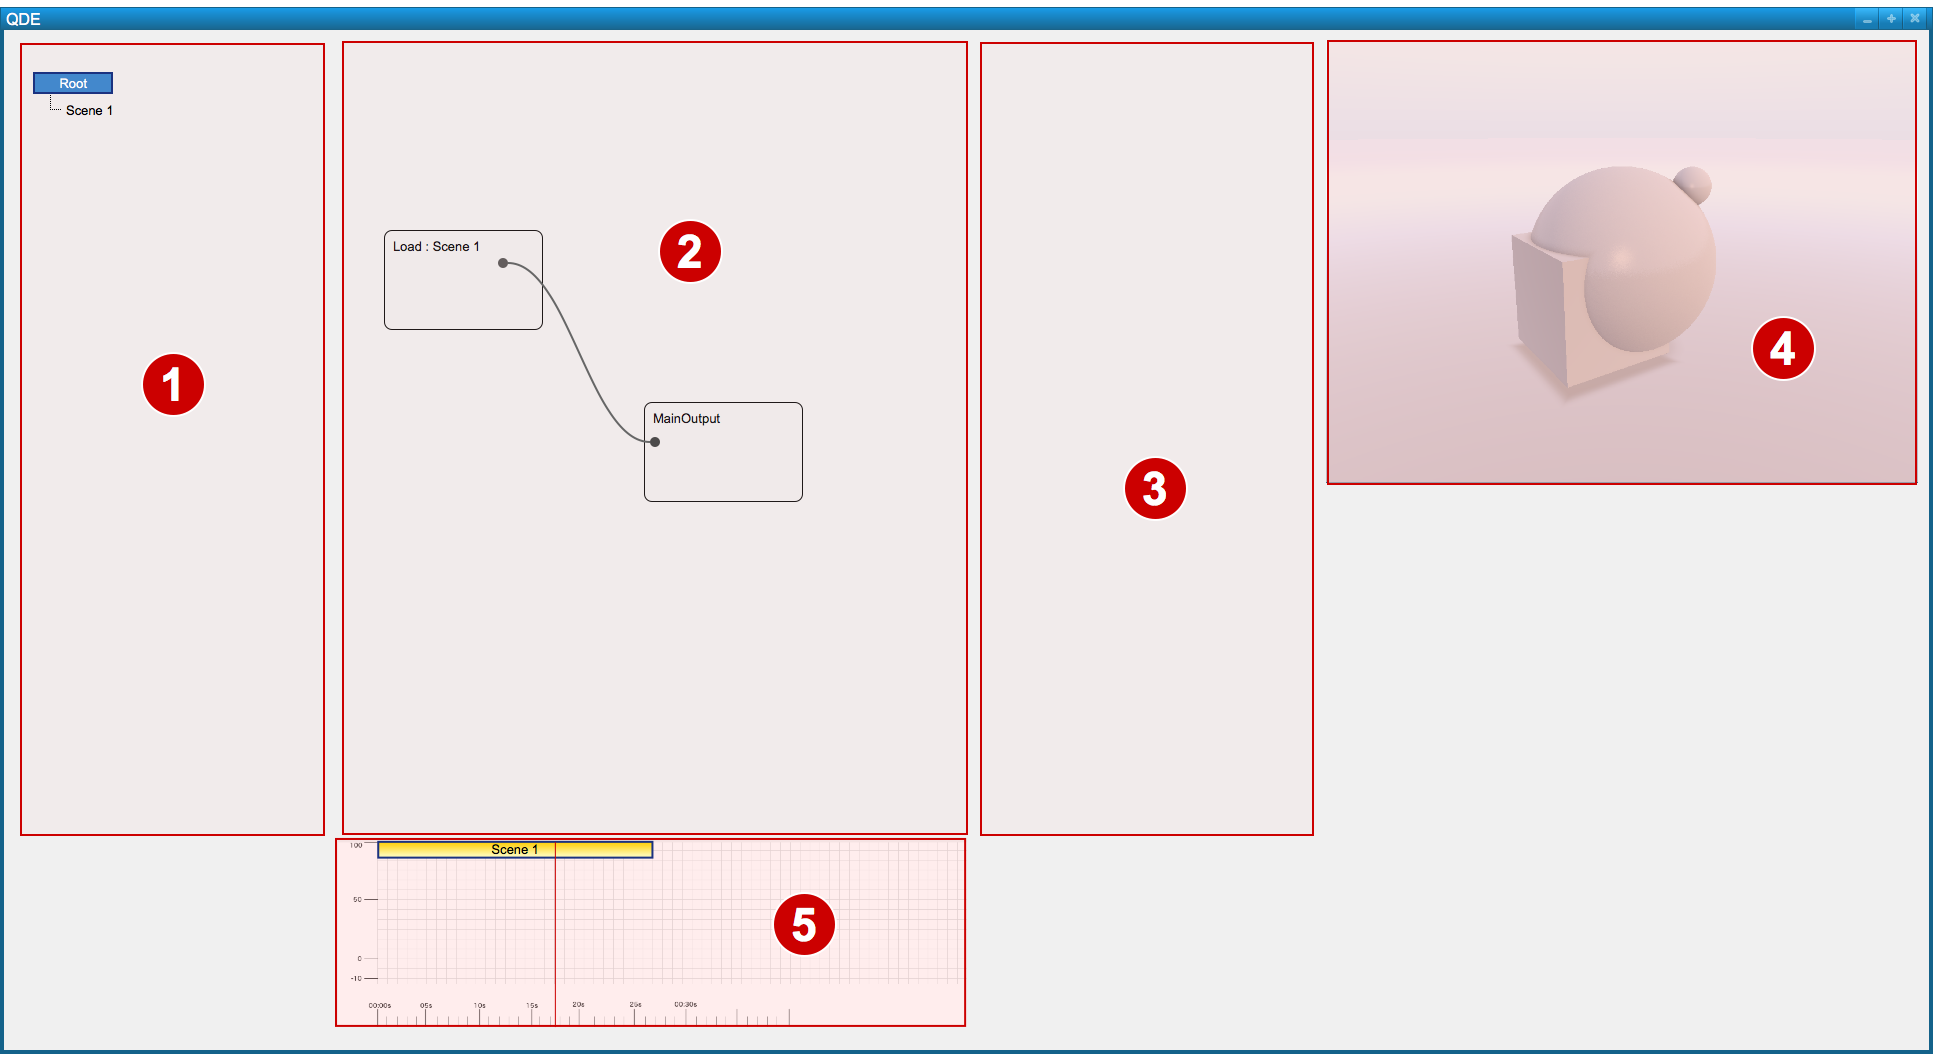
\includegraphics[width=0.95\linewidth]{images/editor-components}
\end{figure}

\newthought{Identifying the components} helps finding the important conceptual items.
Decomposing a domain into noteworthy concepts is~\enquote{the quintessential object-oriented analysis
step}~\cite{larman-applying-2004}.~\enquote{The domain model is a visual
representation of conceptual classes or real-situation objects in a
domain.}~\cite{larman-applying-2004}

\newthought{The editor and player components} are shown
in~\autoref{fig:editor-domain-model} and in~\autoref{fig:player-domain-model}
respectively in the form of a domain model. Each domain model is composed of
components which build the sub components of the parent component, in this case
the editor and player. These sub components represent the objects of the
respective domain.

\begin{figure*}[h]
  \caption{Domain model of the editor component.}
  \label{fig:editor-domain-model}
  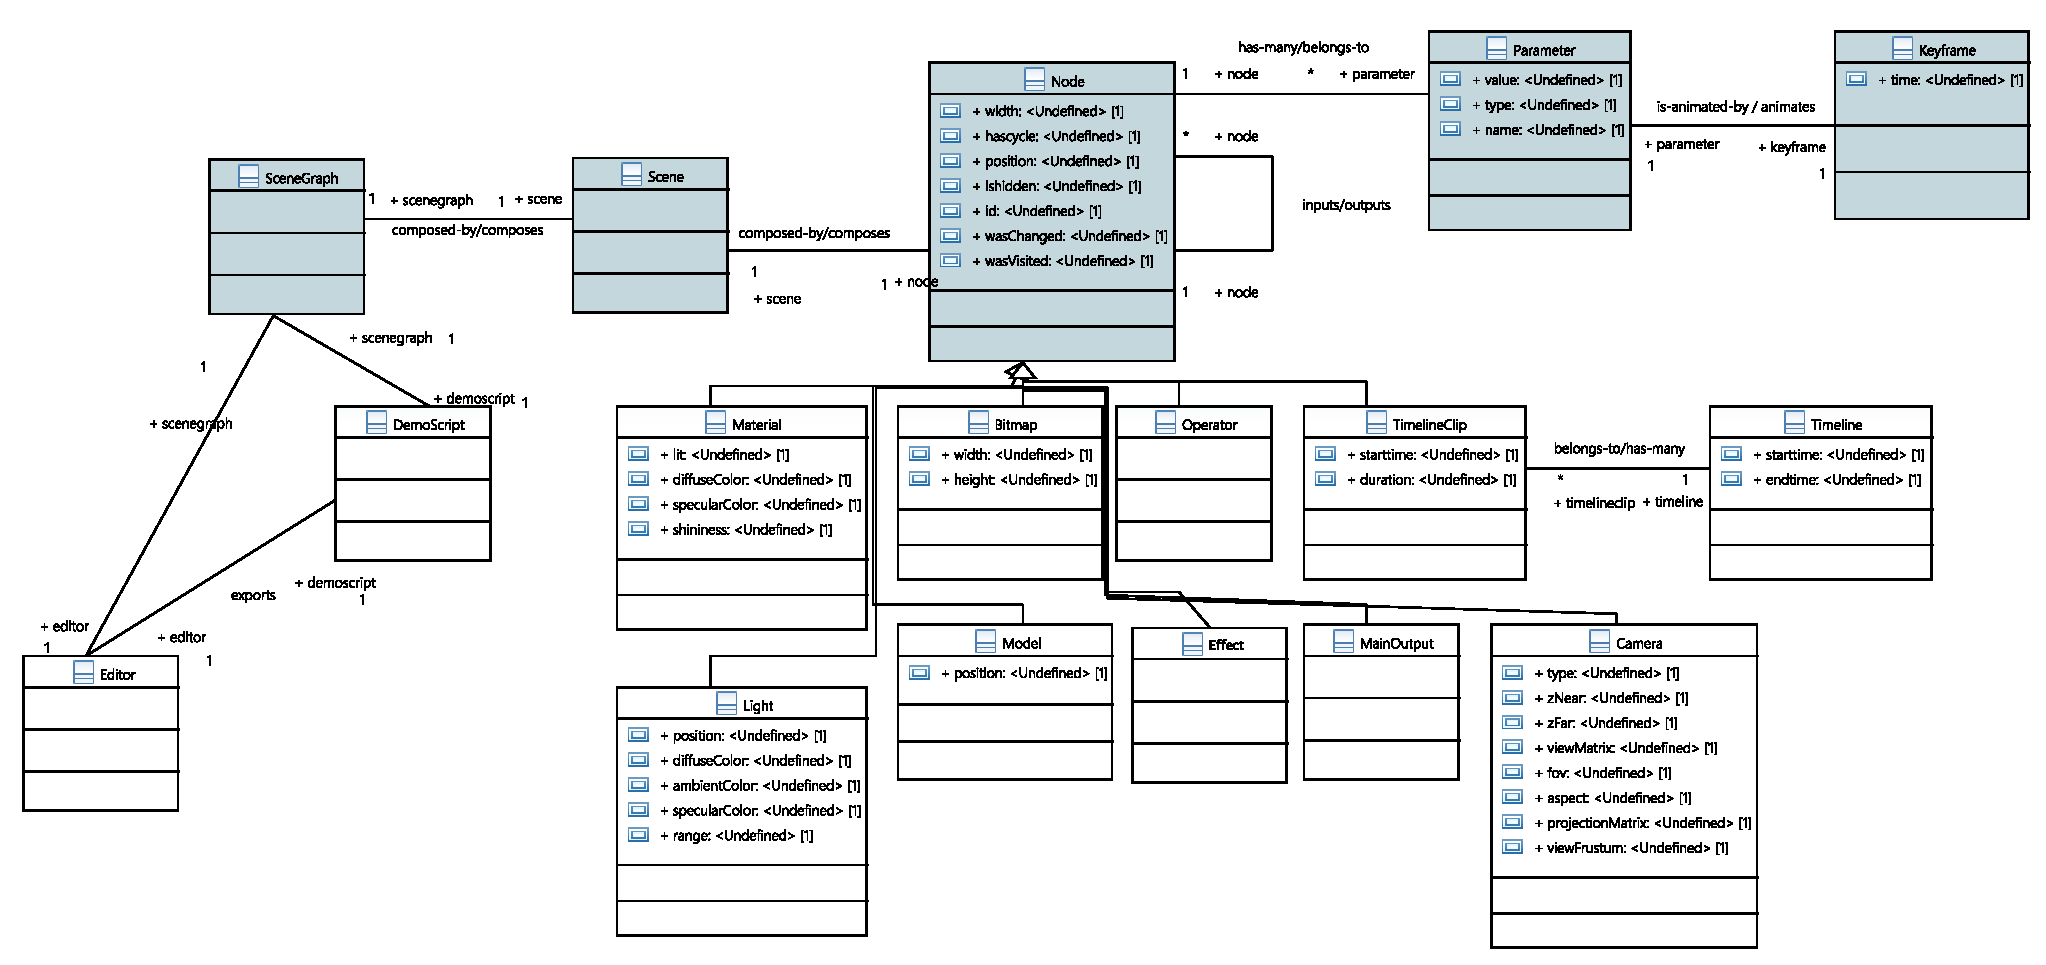
\includegraphics[width=0.95\linewidth]{images/editor-domain-model}
\end{figure*}

\begin{figure*}[ht]
  \caption{Domain model of the player component.}
  \label{fig:player-domain-model}
  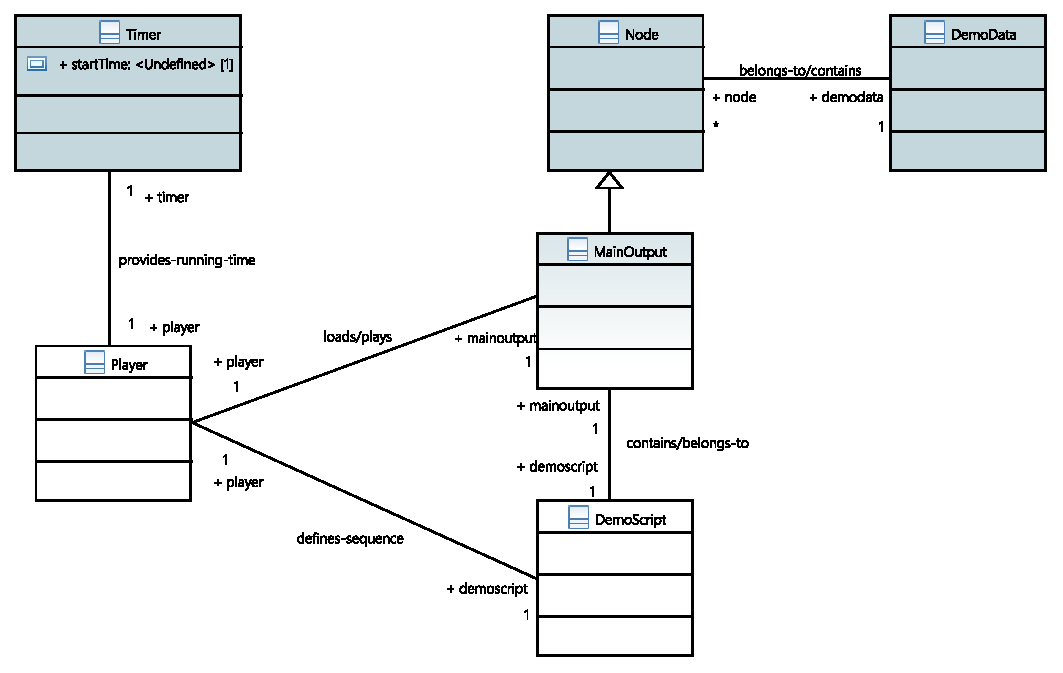
\includegraphics[width=0.95\linewidth]{images/player-domain-model}
\end{figure*}

% TODO: Add may be a reference to the documentation? The image of the editor
% domain model is too small to be read. --> Bigger, scaled and rotated. One
% figure per page.

\newthought{Identifying the important concepts} allows the
definition of the logical architecture and shows the overall image of
(software) classes in form of packets, subsystems and layers. For a detailed
definition of these items the reader is referred to the previous project
work~\cite[pp. 37 ff.]{osterwalder-volume-2016}.

\newthought{To reduce dependencies and the coupling} of components
a~\enquote{relaxed layered} architecture is used. In contrast to a strict
layered architecture, which allows any layer to call services or interfaces only
from the layer below, a relaxed layered architecture allows higher layers to
communicate with any lower layer. The architecture defines five layers, as shown
in~\autoref{table:layers}.

\newthought{To ensure low coupling and dependencies} also for the graphical user
interface, the models and their views are segregated using the principle of
model-view separation which states that domain objects, which are data models,
should have no direct knowledge about their corresponding objects of the
graphical user interface.

\newthought{Workflow objects} control the user interaction with the visual
objects by keeping track of the data models. Such~\textit{controllers} support the
model-view separation principle and exist in the application layer.

\begin{table}[h]
  \caption{Layers as envisaged during the conceptual phase and used for
    the program implemented.}
  \label{table:layers}
  \begin{tabularx}{\textwidth}{lX}
    \toprule
    \textbf{Layer} & \textbf{Description}\\
    \midrule
    UI                 & All elements of the graphical user interface.                                       \\
    Application        & Controllers (workflow objects).                                                     \\
    Domain             & Data models according to the logic of the application.                              \\
    Technical services & Technical infrastructure, such as graphics, window creation and so on.              \\
    Foundation         & Basic elements and low level services, such as timer, arrays or other data classes. \\
    \bottomrule
  \end{tabularx}
\end{table}

\newthought{Class diagrams are used to provide a software point of view},
whereas domain models provide rather a conceptual point of view. A class
diagram~\footnote{The concepts of RUP and OOP are as used in the previous
project (QDE) and therefore will not be detailed here.} shows classes,
interfaces and their relationships.~\autoref{fig:editor-class-diagram} shows the
class diagram of the editor component and~\autoref{fig:player-class-diagram}
shows the class diagram for the player component.

\begin{figure*}[ht]
  \caption{Class diagram of the editor component.}
  \label{fig:editor-class-diagram}
  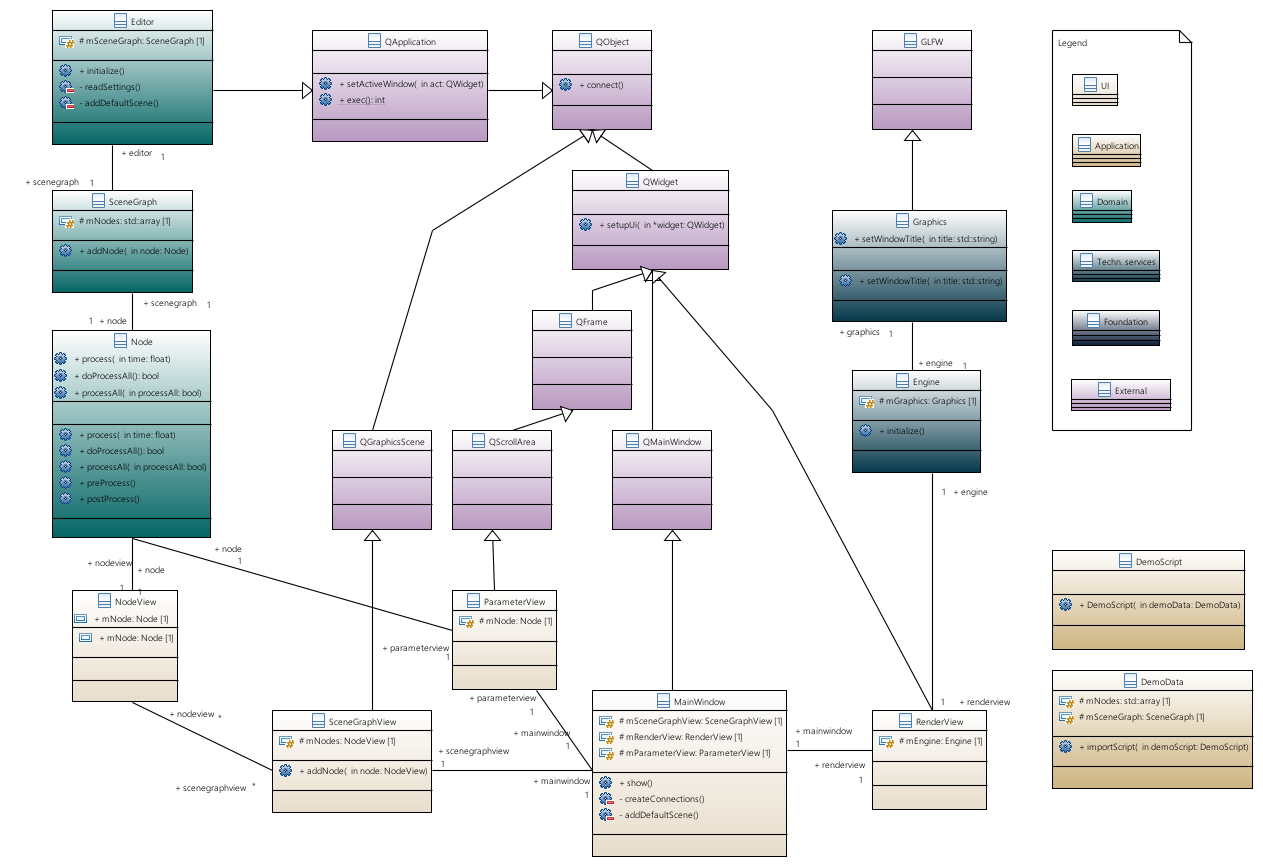
\includegraphics[width=0.95\linewidth]{images/editor-class-diagram}
\end{figure*}

\begin{figure*}[ht]
  \caption{Class diagram of the player component.}
  \label{fig:player-class-diagram}
  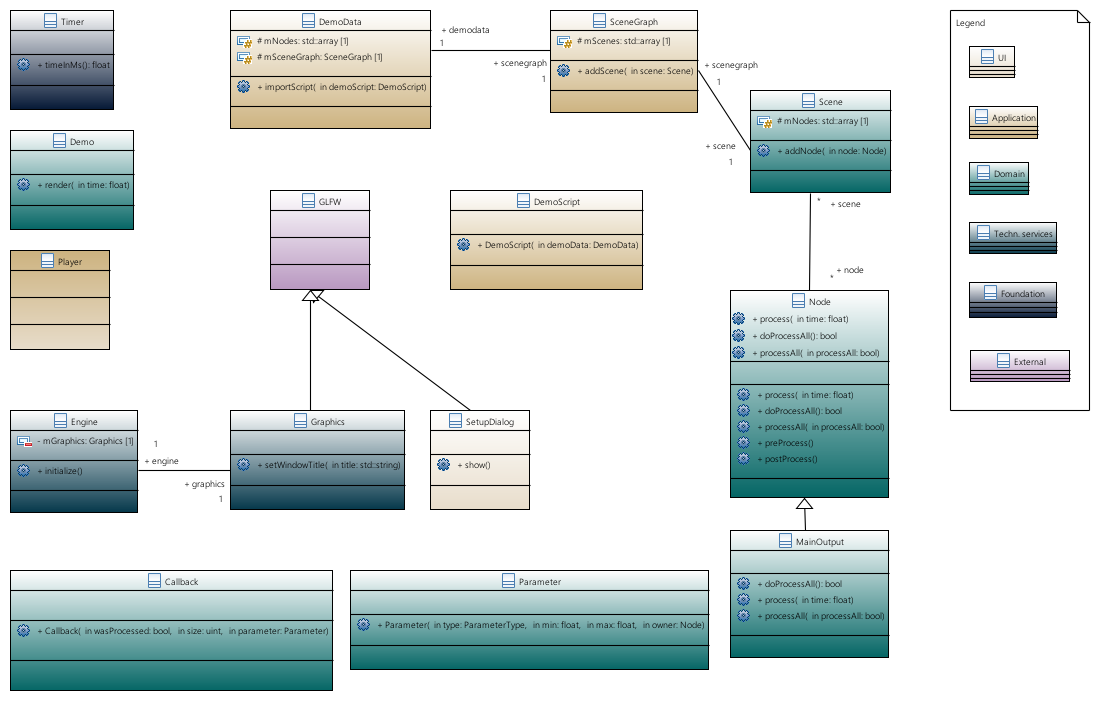
\includegraphics[width=0.95\linewidth]{images/player-class-diagram}
\end{figure*}

% TODO: Add may be a reference to the documentation? The images of the class
% diagrams are too small to be read. --> Bigger, scaled and rotated. One figure
% per page.

\section{Rendering}
\label{sec:rendering}

\newthought{This~\autoref{sec:rendering}} is a summary of the previous project
work of the author,~\enquote{Volume ray casting --- basics \&
principles}~\cite{osterwalder-volume-2016}. It describes the fundamentals for
the rendering algorithm that is used for the program implemented in this thesis.

\newthought{Rendering} is the second main aspect of this thesis, as the
objective is the design and development of a program for modeling, composing and
\textit{rendering} real time computer graphics by providing a graphical toolbox.

\newthought{\citeauthorfin{foley_computer_1996} describes rendering}
as a~\enquote{process of creating images from
models}~\cite{foley_computer_1996}. The basic idea of rendering is to determine
the color of a surface at each point. For this task two concepts have
evolved: \textit{illumination models} and \textit{shading models}.

\newthought{Illumination models} describe the amount of light that is
transmitted from a point on a surface to a viewer. There exist two kinds of
illumination models: local illumination models and global illumination models.
Whereas local illumination models aggregate local data from adjacent surfaces
and directly incoming light from light sources, global illumination models
consider also indirect light from reflections and refractions. The algorithm
used for rendering in the implemented program uses a \textit{global illumination
model}.

\newthought{Shading models} define when and how to use which illumination model.

\newthought{Global illumination models}~\enquote{express the light being
transferred from one point to another in terms of the intensity of the light
emitted}~\cite[pp. 775 and 776]{foley_computer_1996}. Additionally to this
direct intensity, the indirect intensity is considered, meaning~\enquote{the
intensity of light emitted from all other points that reaches the first and is
reflected from the first to the second}~\cite[pp. 775 and
776]{foley_computer_1996} point is added.

\newpage{}

\newthought{In 1986 James Kajiya} set up the so called rendering equation, which
expresses this behavior.~\parencites{kajiya_rendering_1986}[p.
776]{foley_computer_1996}

\begin{figure}
  \label{eq:rendering-equation}
  \caption{The rendering equation as defined by James~\enquote{Jim} Kajiya.}
  \begin{equation}
    I(x, x') = g(x, x')\left[\varepsilon(x, x') + \int\limits_{S}\rho(x, x', x'')I(x', x'')dx''\right]
  \end{equation}
\end{figure}

\marginnote{%-130pt
  \begin{description}
    \item[$x, x' \text{and } x''$] Points in space.
    \item[$I(x, x')$] Intensity of the light going from point $x'$ to point $x$.
    \item[$g(x, x')$] A geometrical scaling factor:
      \begin{itemize}
        \item[--] $0$ if $x$ or $x'$ are occluded by each other.
        \item[--] $\frac{1}{r^2}$ if $x$ and $x'$ are visible to one other, $r$ being
          the distance them.
      \end{itemize}
    \item[$\varepsilon(x, x')$] Intensity of the light being emitted from point
      $x'$ to point $x$.
    \item[$\rho(x, x', x'')$] Intensity of the light going from $x''$ to $x$, being
      scattered on the surface near point $x'$.
    \item[$\int\limits_{S}$] Integral over the union of all surfaces, hence $S =
      \bigcup\limits_{i=0}^{n} S_{i}$, $n$ being the number of surfaces.
      All points $x$, $x'$ and $x''$ brush all surfaces of all objects within
      the scene. Where $S_{i}$ is the surface of object $i$, and so $S_{0}$
      being an additional surface in form of a hemisphere which spans the whole
      scene and acts as background.
  \end{description}
}

% \begin{table}[h]
%   \caption{Description of the single aspects of the rendering equation.}
%   \begin{tabularx}{\textwidth}{lX}
%     \toprule
%     \textbf{Part} & \textbf{Description} \\
%     \midrule
%     $x, x' \text{and } x''$ & Points in space. \\
%     \midrule
%     $I(x, x')$ & Intensity of the light going from point $x'$ to point $x$. \\
%     \midrule
%     $g(x, x')$ & A geometrical term. \newline
%         \hspace*{4mm} $0$: \hspace*{2mm} $x$ and $x'$ are occluded by each other.
%         \newline
%         \hspace*{4mm} $1\over{r^2}$: \hspace*{1mm} $x$ and $x'$ are visible to one
%         other, $r$ being the \newline
%         \hspace*{12mm} distance between the two points. \\
%     \midrule
%     $\varepsilon(x, x')$ & Intensity of the light being emitted from point $x'$
%     to point $x$. \\
%     \midrule
%     $\rho(x, x', x'')$ & Intensity of the light going from $x''$ to $x$, being
%     scattered on the surface of point $x'$. \\
%     \midrule
%     $\int\limits_{S}$ & Integral over the union of all surfaces, hence $S =
%     \bigcup\limits_{i=0}^{n} S_{i}$, $n$ being the number of
%     surfaces.
%     All points $x$, $x'$ and $x''$ brush all surfaces of all objects within the
%     scene. $S_{0}$ being an additional surface in form of a hemisphere which
%     spans the whole scene and acts as background.\\
%     \bottomrule
%   \end{tabularx}
% \end{table}

\newthought{Implementing a global illumination model} or the rendering equation
directly for rendering images in viable (computational feasible in a workflow
for instance for the production of animated films) or even real time is not
really feasible, even on the fastest modern hardware (2017). The procedure is
computationally complex and very time demanding.

\newthought{A simplified approach} to implement global illumination models (and
the rendering equation) is ray tracing. Ray tracing is able to produce high
quality, realistic looking images. Although it is still demanding in terms of
time and computations, the time complexity is viable for producing still
images. For producing images in real time however, the algorithm is still too
demanding. This is where a special form of ray tracing comes in.

\newthought{Sphere tracing} is a ray tracing approach for implicit surfaces
introduced in~\citeyear{hart_sphere_1994} by~\citeauthorfin{hart_sphere_1994} in
his work~\citetitle{hart_sphere_1994}~\cite{hart_sphere_1994}. 
Sphere tracing is faster than the classical ray tracing approaches in its method
of finding
intersections between rays and objects. In contrast to the classical ray tracing
approaches, the~\enquote{marching distance} of rays is not defined by an absolute or a
relative distance, but instead, distance functions are used. The distance functions
are used to expand unbounding volumes (in this concrete case spheres, hence the
name) along rays.~\autoref{fig:sphere-tracing-1} illustrates this procedure.

\begin{figure}[h]
    \centering
    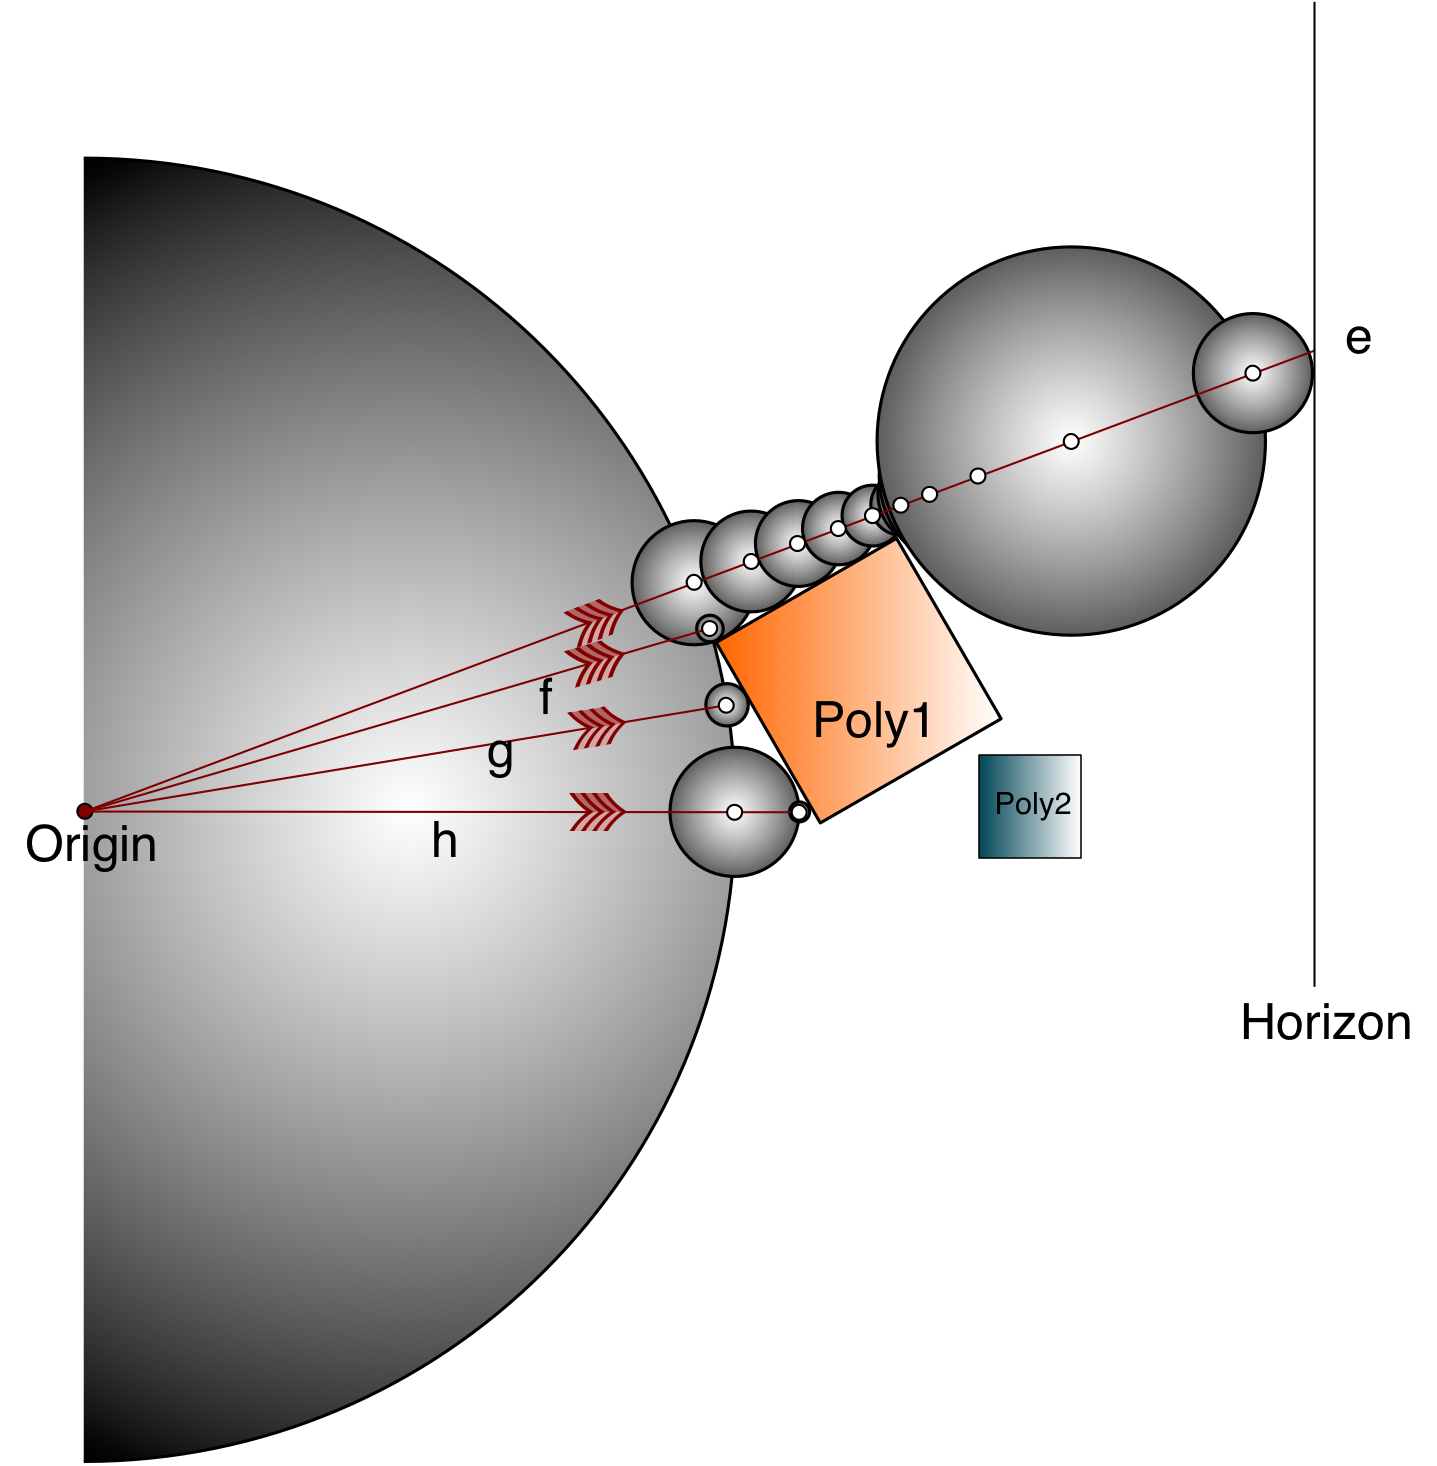
\includegraphics[width=0.75\linewidth]{images/sphere-tracing-principle}
    \caption{Illustration of the sphere tracing
      algorithm.
      Ray~\textit{e} hits no objects until reaching the horizon.
      Rays~\textit{f},~\textit{g} and~\textit{h} hit
      the solid~\textit{poly1}.}
      \label{fig:sphere-tracing-1}
\end{figure}

\newthought{Bounding volumes} are defined as the enclosure of a sold. On the
other hand, unbounding volumes are the space outside of a bounding volume,
including the surface of the solid itself. For calculating a unbounding volume,
the distance between an object and any defined origin point is evaluated. If
this distance is known, it can be taken as the radius of a sphere centered at
the origin point.

\newthought{Sphere tracing} defines objects as implicit surfaces using distance
functions. Therefore the distance from every point in space to every other point
in space and to every surface of every object can be calculated. These distances
build a so called distance field.

\newthought{The sphere tracing algorithm} is as follows. A ray is shot
from an origin point (for example, the viewer such as an eye or a pinhole camera) into a scene.
The radius of an unbounding volume in form of a sphere is calculated from
the origin, as described above. They ray intersects with the sphere, which gives
the distance that the ray will travel in a first step. From this
intersection the next unbounding volume (sphere) is expanded and its radius is
calculated, which gives the next intersection of the ray. This procedure
continues until an object is hit or until a predefined maximum distance of
the ray is being reached, defined as the~\enquote{horizon}. An object is
considered as~\enquote{hit} whenever the
returned radius of the distance function is below a predefined constant
$\epsilon$, the~\enquote{convergence precision}.

\newthought{A possible implementation} of the sphere tracing algorithm is shown
in~\autoref{alg:sphere-tracing}, although this shows only the distance
estimation. Shading is done in another implementation, for example in a
render method which calls the sphere trace method. Shading means in this context
the determination of the color of a surface or pixel.

\begin{figure*}
  \label{alg:sphere-tracing}
  \caption{%
    An abstract implementation of the sphere tracing algorithm. Algorithm in
    pseudo code, after~\cite{hart_sphere_1994}[S. 531, Fig. 1]
  }
  \begin{pythoncode}
def sphere_trace():
    ray_distance          = 0
    estimated_distance    = 0
    max_distance          = 9001
    max_steps             = 100
    convergence_precision = 0.000001

    while ray_distance < max_distance:
        # sd_sphere is a signed distance function defining the implicit surface.
        # cast_ray defines the ray equation given the current traveled /
        # marched distance of the ray.
        estimated_distance = sd_sphere(cast_ray(ray_distance))

        if estimated_distance < convergence_precision:
            # the estimated distance is already smaller than the desired
            # precision of the convergence, so return the distance the ray has
            # travelled as we have an intersection
            return ray_distance

        ray_distance = ray_distance + estimated_distance

    # When we reach this point, there was no intersection between the ray and a
    # implicit surface, so simply return 0
    return 0
  \end{pythoncode}
\end{figure*}

\newthought{Shading} is done as proposed by~\citeauthorfin{whitted_improved_1980}
in~\citetitle{whitted_improved_1980}~\cite{whitted_improved_1980}. This means,
that the sphere tracing algorithm must return which object was hit and its material.
Depending on the material, four cases can occur. The material may be:
\begin{enumerate*}
  \item reflective and refractive,
  \item reflective only,
  \item diffuse or
  \item emissive.
\end{enumerate*}
For simplicity only the third case is being taken into account. For the actual
shading a local illumination method is used, called~\textit{Phong shading}.

\newthought{The Phong illumination model}~\cite[p. 123]{foley_computer_1996} describes (reflected) light intensity
$I$ as a composition of the ambient, the diffuse and the perfect specular
reflection of a surface.

\begin{figure}
  \label{eq:phong-equation}
  \caption{%
    The Phong illumination model as defined by Phong Bui-Tuong.~\cite[p. 123]{foley_computer_1996} Note that
    the emissive term was left out intentionally as it is mainly used to achieve
    special effects.\newline{}
    \newline{}
    Foo.
  }
  \begin{equation}
    I(\vv{V}) = k_{a} \cdot L_{a} + k_{d} \displaystyle\sum_{i=0}^{n - 1} L_{i} \cdot (\vv{S_{i}} \cdot \vv{N}) + k_{s} \displaystyle\sum_{i=0}^{n - 1} L_{i} \cdot {(\vv{R_{i}} \cdot \vv{V})}^{k_{e}}
  \end{equation}
\end{figure}

% \marginnote[-130pt]{
\marginnote{
  \begin{description}
    \item[$I(x, x')$] Intensity of the light at point $\vv{V}$.
    \item[$k_{a}$] A constant defining the ratio of reflection of the ambient
      term of all points in the scene.
    \item[$L_{a}$] Intensity of the ambient light.
    \item[$k_{d}$] A constant defining the ratio of the diffuse term of incoming
      light.
    \item[$\displaystyle\sum_{i=0}^{n-1}$] Sum over all light sources in the scene.
    \item[$L_{i}$] Intensity of the~\emph{i}-th light source.
    \item[$\vv{S_{i}}$] Direction vector from the point on the surface toward
      light source~\emph{i}.
    \item[$\vv{N}$] Normal vector at the point of the surface.
    \item[$\vv{R_{i}}$] Direction that a perfectly reflected ray of light would
      take from this point on the surface.
    \item[$\vv{V}$] Direction pointing toward the viewer.
    \item[$k_{e}$] Shininess constant for the material.
  \end{description}
}% -*- mode: latex; coding: utf-8; outline-minor-mode: t -*-

\chapter{Methodologies}
\label{chap:methodologies}

% Das Kapitel der Methoden erklärt, was (Material) untersucht wurde und wie
% (Methode) ersteres untersucht wurde. Aufgrund der Beschreibung der Methoden muss
% es möglich sein, den Versuch oder die Studie zu wiederholen. Ist die
% Beschreibung der Versuchsanordnung oder des Vorgehens von sehr geringem Umfang,
% können diese nach Rücksprache mit der Betreuungsperson auch als Absatz in der
% Einleitung oder als Unterkapitel zum Kapitel der Einleitung verfasst werden.

% Link to previous
% Make a connection to what has immediately gone before. Recap the last chapter.
% In the last chapter I showed that… Having argued in the previous chapter that…
% As a result of x, which I established in the last chapter….. It is also possible
% to make a link between this chapter and the whole argument… The first step in
% answering my research question (repeat question) .. was to.. . In the last
% chapter I …
\newthought{The previous chapter} provided the fundamentals that are required for
understanding the results of this thesis.

% Focus: What does this chapter specifically do?
% Now focus the reader’s attention on what this chapter is specifically going to
% do and why it is important. In this chapter I will examine.. I will present… I
% will report … This is crucial in (aim of thesis/research question) in order to….
\newthought{This chapter} presents the methodologies that are used to implement
this thesis.

% Overview: How is it done?
% The third paragraph simply outlines the way that you are going to achieve the
% aim spelled out in the previous paragraph. It’s really just a statement of the
% contents in the order that the reader will encounter them. It is important to
% state these not simply as topics, but actually how they build up the internal
% chapter argument… I will begin by examining the definitions of, then move to
% seeing how these were applied… I first of all explain my orientation to the
% research process, positioning myself as a critical scholar.. I then explain the
% methodology that I used in the research, arguing that ethnography was the most
% suitable approach to provide answers to the question of…
\newthought{The first section of this chapter} shows a principle called literate
programming, which is used to generate this documentation and the practical
implementation in terms of a software. The second section describes the agile
methodologies, that are used to implement this thesis.

\section{Literate programming}
\label{sec:literate-programming}

\newthought{Software may be documented in different ways.} It may be in terms of
a documentation, e.g. in the form of a software architecture which
describes the software conceptually and hints at its implementation. Or it may
be in terms of documenting within the software itself through inline comments.
Frequently both methodologies are used. However, all too
frequently the documentation is not done properly, and even neglected as it can
be quite costly with seemingly little benefit.

\newthought{Documenting software is critical.} Whenever software is written,
decisions are made. In the moment a decision is made, it may seem intuitively
clear, as it has evolved through creative thought processes. The seeming clarity
of the decision is most of the time deceptive. Is a decision still clear when
some time has passed since making that decision? What were the considerations
that led to it? Is the decision also clear for other, may be less-involved
persons? All these concerns show that documenting software is critical. No
documentation at all, or outdated or irrelevant documentation, can lead to
unforeseen and costly efforts concerning work and time.

\newthought{\citeauthorfin{hoare-hpl-1973} states~\citeyear{hoare-hpl-1973}} in his
work~\citetitle{hoare-hpl-1973} that~\enquote{documentation must be regarded as
an integral part of the process of design and coding}~\cite[p.
195]{hoare-hpl-1973}: ~\enquote{The purpose of program documentation is to
explain to a human reader the way in which a program works so that it can be
successfully adapted after it goes into service, to meet the changing
requirements of its users, or to improve it in the light of increased knowledge,
or just to remove latent errors and oversights. The view that documentation is
something that is added to a program after it has been commissioned seems to be
wrong in principle and counter-productive in practice. Instead, documentation
must be regarded as an integral part of the process of design and coding. A good
programming language will encourage and assist the programmer to write clear
self-documenting code, and even perhaps to develop and display a pleasant style
of writing. The readability of programs is immeasurably more important than
their writeability.}~\cite[p. 195]{hoare-hpl-1973}

\newthought{Literate programming}, a paradigm proposed
in~\citeyear{knuth-lp-1984} by~\citeauthorfin{knuth-lp-1984}, goes even further.
\citeauthorfin{knuth-lp-1984} believes that \enquote{significantly better
documentation of programs} can be best achieved~\enquote{by considering programs
to be works of literature}~\cite[p.
1]{knuth-lp-1984}.~\citeauthorfin{knuth-lp-1984} proposes to change
the~\enquote{traditional attitude to the construction of programs}~\cite[p.
1]{knuth-lp-1984}. Instead of imagining that the main task is to instruct a
computer what to do, one should concentrate on explaining to human beings what
the computer shall do.~\cite[p. 1]{knuth-lp-1984}

\newthought{The ideas of literate programming} have been embodied in several
software systems, the first being~\emph{WEB}, introduced
by~\citeauthorfin{knuth-lp-1984} himself. These systems are a combination of two
languages:
\begin{enumerate*}
  \item a document formatting language and
  \item a programming language
\end{enumerate*}.
Such a software system uses a single document as input (which can be split up in
multiple parts) and generates two outputs:
\begin{enumerate*}
  \item a document in a formatting language, such as
    Knuth's~\LaTeX{}~\cite{knuth-tex-1987} (which may then be converted in a
    printable and viewable form, such as PDF).
  \item a compilable program in a programming language, such as Python or C
    (which may then be converted into an executable program).
\end{enumerate*}~\cite{knuth-lp-1984}
The first process is called~\emph{weaving} and the second~\emph{tangling}. This
process is illustrated in~\autoref{fig:weave-and-tangle}.

\begin{figure}
  \label{fig:weave-and-tangle}
  \caption{Illustration showing the processes of~\emph{weaving}
    and~\emph{tangling} documents from a input document.~\cite{knuth-lp-1984}}
  \begin{tikzpicture}
    \begin{scope}[every node/.style={minimum size=4em,circle,thick,draw}]
      \node (input) at (0,  0) {Input};
      \node (tex)   at (3,  2) {file.tex};
      \node (c)     at (3, -2) {file.c};
      \node (pdf)   at (8,  2) {file.pdf};
      \node (bin)   at (8, -2) {binary};
    \end{scope}
    \begin{scope}[>={Stealth[black]},
      every node/.style={fill=white,circle},
      every edge/.style={draw=black,thick}]
      \path [->] (input) edge[bend left=30] node {weave} (tex);
      \path [->] (input) edge[bend right=30] node {tangle} (c); 
      \path [->] (tex) edge node {convert} (pdf); 
      \path [->] (c) edge node {compile} (bin); 
    \end{scope}
  \end{tikzpicture}
\end{figure}

\newthought{Several literate programming (LP) systems were evaluated} during the
first phase of this thesis:
CWEB~\sidenote{\url{http://www-cs-faculty.stanford.edu/~uno/cweb.html}},
Noweb~\sidenote{\url{https://www.cs.tufts.edu/~nr/noweb/}},
lit~\sidenote{\url{http://cdosborn.github.io/lit/lit/root.html}},
PyLiterate~\sidenote{\url{https://github.com/bslatkin/pyliterate}},
pyWeb~\sidenote{\url{http://pywebtool.sourceforge.net/}} and
Babel~\sidenote{\url{http://orgmode.org/worg/org-contrib/babel/}}. All of these
tools have their strengths and weaknesses.
However, none of these systems fulfill all the needed requirements of this
project:
\begin{enumerate*}
  \item Provide \enquote{pretty printing}~\protect\footnotemark[1]{} of the program parts.
  \item Provide automatic references between the definition of program parts and
    their usage.
  \item Expand program parts having the same name instead of redefining them.
  \item Support Python as programming language.
  \item Allow the inclusion of files for both parts, the document formatting
    language and the programming language.
\end{enumerate*}
\footnote{pretty printing refers to content-based formatting (e.g. line color
  and indentation to improve readability).}

\newthought{Ultimately a further literate programming system},
nuweb~\footnote{\url{http://nuweb.sourceforge.net/}}, was chosen as it fulfills
all these requirements. It has adapted and simplified the ideas of
FunnelWeb~\footnote{\url{http://www.ross.net/funnelweb/}}. It is independent of
the programming language for the source code. As document formatting language it
uses~\LaTeX{}. Although the documentation of nuweb states that it is not
designed for the pretty printing of source code, it does provide an option to
display source code as listings. This facility has been modified to support
visualizing the expansion of parts as well as to use syntax highlighting of the
code within~\LaTeX{}.

\newthought{The nuweb system provides several commands to process files.} All
commands begin with an at sign (@). Whenever a file or part does not contain
any commands the file is copied unprocessed. nuweb provides a single executable
program, which processes the input files and generates the output files (weaving
and tangling, in document formatting language and as source code respectively).

\newthought{A fragment consists of scraps} which in this project contain the
source code. They may also contain for instance paragraphs for formatted text or
mathematical equations.

\newthought{Literate programming can be very expressive} when all concepts are
explicitly defined before implementation.~\citeauthorfin{knuth-lp-1984} sees this
expressiveness an advantage as one is forced to clarify thoughts before
programming~\cite[p. 13]{knuth-lp-1984}. This is surely very true for small
software but only partly true for larger software. The problem with larger
software is, that when using literate programming, the documentation tends to be
correspondingly large. \emph{To overcome this problem} in this project, the
actual implementation of the software is placed into to the
appendix~\todo{insert reference to appendix here}.

\newthought{Another problematic aspect} is the implementation of repeating
fragments or parts with similar but not identical technical details (such as imports
or getter and setter methods). This might be interesting only for
software developers or technically oriented readers who want to grasp all the
details.~\emph{This aspect can
be overcome} by moving recurring or uninteresting fragments to a separate
file (see~\todo{add reference to code fragments}).

\newthought{To show the principles of literate programming},
without annoying the reader, only an excerpt of some details is given here.

\newthought{One of the more interesting things} of the software might
be the definition of a node~\todo{add reference to the node concept within
appendix} and its loading from external files. These two aspects are shown
below. More details of this example would go beyond the scope of this thesis.

\newthought{Some essential thoughts about classes and objects} may help to stay
consistent when developing the software, before implementing the node class.
Each class should at least have four parts:
\begin{enumerate}
  \item Signals --- to inform other objects about events.
  \item A constructor --- creator of an initial instance of a class.
  \item Various methods --- actions which can be executed by the object.
  \item Slots --- receive signals from other objects.
\end{enumerate}
This structure is applied to the declaration of the node class.

\newpage{}

\newthought{Implementing the node class} means simply defining a~\emph{scrap}
called~\enquote{\emph{Node definition declaration}} using the above pattern.
The~\emph{scrap} does not have any content at the moment, except references to
other scraps, which build the body of the scrap and which will be defined later
on.

\begin{figure}[h]
  \begin{flushleft} \small
\begin{minipage}{\linewidth}\label{scrap1}\raggedright\small
\NWtarget{nuweb?}{} $\langle\,${\itshape Node definition declaration}\nobreak\ {\footnotesize {?}}$\,\rangle\equiv$
\vspace{-1ex}
\begin{pythoncode}
class NodeDefinition(object):
    """Represents a definition of a node."""

    # Signals
    |\hbox{$\langle\,${\itshape Node definition signals}\nobreak\ {\footnotesize ?}$\,\rangle$}|
    |\hbox{$\langle\,${\itshape Node definition constructor}\nobreak\ {\footnotesize \NWlink{nuweb?}{?}}$\,\rangle$}|
    |\hbox{$\langle\,${\itshape Node definition methods}\nobreak\ {\footnotesize ?}$\,\rangle$}|

    # Slots
    |\hbox{$\langle\,${\itshape Node definition methods}\nobreak\ {\footnotesize ?}$\,\rangle$}||\NWsep|
\end{pythoncode}
\vspace{1.5ex}
\footnotesize
\begin{list}{}{\setlength{\itemsep}{-\parsep}\setlength{\itemindent}{-\leftmargin}}
\item {\NWtxtMacroNoRef}.

\item{}
\end{list}
\end{minipage}\vspace{4ex}
\end{flushleft}
\caption{Declaration of the node definition class.}
  \label{lst:node-def-class-decl}
\end{figure}

\newthought{The constructor} might be the first thing to implement, following
the developed pattern. In Python the constructor defines the properties of a
class~\sidenote[][-10pt]{Properties do not need to be defined in the constructor,
they may be defined anywhere within the class. However, this can lead to
confusion and it is therefore considered as good practice to define the
properties of a class in its constructor.}, therefore it defines what a class
actually is or represents --- the concept. After some thinking, and in context
of the intended software, one might come up with the properties
in~\autoref{table:node-properties} defining a node definition.

\begin{table*}[!htp]
  \begin{tabularx}{\linewidth}{lX}
    \toprule
    \textbf{Property} & \textbf{Description}\\
    \midrule
    ID          & A globally unique identifier for the node definition.          \\
    Name        & The name of the definition.                                    \\
    Description & The description of the definition. What does that definition
                  provide?                                                       \\
    Parent      & The parent object of the current node definition.              \\
    Inputs      & Inputs of the node definition. This may be distinct types or
                  references to other nodes.                                     \\
    Outputs     & The same as for inputs.                                        \\
    Invocation  & A list of the node's invocations or calls respectively.        \\
    Parts       & Defines parts that may be processed when evaluating the node.
                  Contains code which can be interpreted directly.               \\
    Connections & A list of connections of the node's inputs and outputs. Each
                  connection is composed by two parts:
                  \begin{enumerate*}
                    \item a reference to another node and
                    \item a reference to an input or an output of that node.
                  \end{enumerate*}
                  Is the reference not set, that is, its value is zero, this
                  means that the connection is internal.                         \\
    Instances   & A list of node instances from a certain node definition.       \\
    Was changed & Flag, which indicates whether a definition was changed or not. \\
    \bottomrule
  \vspace*{\baselineskip}
  \caption{Properties/attributes of the node class.}
  \label{table:node-properties}
  \end{tabularx}
\end{table*}

\newthought{Implementing the constructor} of the node definition may now follow
from the properties defined in~\autoref{table:node-properties}. As the name of
the constructor definition was already given, by using it
within~\autoref{lst:node-def-class-decl}
(\verb|@<Node definition constructor@>|), the very same name will be used for
actually defining the scrap itself.

\begin{figure}[!htbp]
  \begin{flushleft} \small
\begin{minipage}{\linewidth}\label{scrap2}\raggedright\small
\NWtarget{nuweb?}{} $\langle\,${\itshape Node definition constructor}\nobreak\ {\footnotesize {?}}$\,\rangle\equiv$
\vspace{-1ex}
\begin{pythoncode}
def __init__(self, id_):
    """Constructor.

    :param id_: the globally unique identifier of the node.
    :type  id_: uuid.uuid4
    """

    self.id_         = id_

    self.name        = ""
    self.description = ""
    self.parent      = None
    self.inputs      = []
    self.outputs     = []
    self.invocations = []
    self.parts       = []
    self.nodes       = []
    self.connections = []
    self.instances   = []
    self.was_changed = False|\NWsep|
\end{pythoncode}
\vspace{1.5ex}
\footnotesize
\begin{list}{}{\setlength{\itemsep}{-\parsep}\setlength{\itemindent}{-\leftmargin}}
\item \NWtxtMacroRefIn\ \NWlink{nuweb?}{?}.

\item{}
\end{list}
\end{minipage}\vspace{4ex}
\end{flushleft}
\caption{Constructor of the node definition class. Note that the
    identifier is given by a corresponding parameter. Identifiers have to be
    generated when defining a node using an external file.}
  \label{lst:node-def-constructor}
\end{figure}

\newthought{One of the problems mentioned before} can be seen
in~\cref{lst:node-def-constructor}: it shows a rather dull constructor without
any logic which is not interesting. Additionally importing of modules would be
needed, e.g. PyQt or system modules. This was left out deliberately. At this
point the implementation of node definitions will not be shown further, as this
is beyond scope. Further implementation can be seen at~\todo{insert
reference(s) to node domain model here}.

\newthought{Node definitions will be loaded from external files} in JSON format.
This happens within the node controller component, which will not be shown here
as this would go beyond the scope. Required attributes will be mentioned
explicitly although. The method for loading the nodes,
\mintinline{python}{load_node_definitions}, defined
in~\cref{lst:load-node-definitions}, does not have any arguments. Everything
needed for loading nodes is encapsulated in the node controller.

\begin{figure}[h]
  \begin{flushleft} \small
\begin{minipage}{\linewidth}\label{scrap3}\raggedright\small
\NWtarget{nuweb?}{} $\langle\,${\itshape Load node definitions}\nobreak\ {\footnotesize {?}}$\,\rangle\equiv$
\vspace{-1ex}
\begin{pythoncode}
def load_node_definitions(self):
    """Loads all files with the ending NODES_EXTENSION
    within the NODES_PATH directory, relative to
    the current working directory.
    """
|\NWsep|
\end{pythoncode}
\vspace{1.5ex}
\footnotesize
\begin{list}{}{\setlength{\itemsep}{-\parsep}\setlength{\itemindent}{-\leftmargin}}
\item \NWtxtMacroDefBy\ \NWlink{nuweb?}{?}\NWlink{nuweb?}{, ?}.
\item {\NWtxtMacroNoRef}.

\item{}
\end{list}
\end{minipage}\vspace{4ex}
\end{flushleft}
\caption{Head of the method that loads node definitions from external JSON
    files.}
  \label{lst:load-node-definitions}
\end{figure}

\newthought{When loading the node definitions}, there are two cases (and
consequences) at the first instance:
\begin{enumerate*}
  \item the directory containing the node definitions exists, the load
    definitions may be loaded or
  \item the directory does not exit.
\end{enumerate*}
In the first case the directory possibly containing node definitions is being
searched for such files, in the second case a warning message is logged.

\begin{figure}[!h]
  \begin{flushleft} \small
\begin{minipage}{\linewidth}\label{scrap4}\raggedright\small
\NWtarget{nuweb?}{} $\langle\,${\itshape Load node definitions}\nobreak\ {\footnotesize {?}}$\,\rangle+\equiv$
\vspace{-1ex}
\begin{pythoncode}
if os.path.exists(self.nodes_path):
    |\hbox{$\langle\,${\itshape Find and load node definition files}\nobreak\ {\footnotesize \NWlink{nuweb?}{?}, \ldots\ }$\,\rangle$}|
else:
    |\hbox{$\langle\,${\itshape Output warning when directory with node definitions does not exist}\nobreak\ {\footnotesize \NWlink{nuweb?}{?}}$\,\rangle$}||\NWsep|
\end{pythoncode}
\vspace{1.5ex}
\footnotesize
\begin{list}{}{\setlength{\itemsep}{-\parsep}\setlength{\itemindent}{-\leftmargin}}
\item \NWtxtMacroDefBy\ \NWlink{nuweb?}{?}\NWlink{nuweb?}{, ?}.
\item {\NWtxtMacroNoRef}.

\item{}
\end{list}
\end{minipage}\vspace{4ex}
\end{flushleft}
\caption{Check whether the path containing the node definition files exist or
    not.}
  \label{lst:nodes-controller-load-nodes-2}
\end{figure}

\newthought{In the first case}, when the directory containing the node
definitions exists, files containing node definitions are searched. The files
are searched by wildcard pattern matching the extension:~\verb|*.node|.

\begin{figure}[!h]
  \begin{flushleft} \small
\begin{minipage}{\linewidth}\label{scrap5}\raggedright\small
\NWtarget{nuweb?}{} $\langle\,${\itshape Find and load node definition files}\nobreak\ {\footnotesize {?}}$\,\rangle\equiv$
\vspace{-1ex}
\begin{pythoncode}
node_definition_files = glob.glob("{path}{sep}*.{ext}".format(
    path=self.nodes_path,
    sep=os.sep,
    ext=self.nodes_extension
))
num_node_definitions = len(node_definition_files)|\NWsep|
\end{pythoncode}
\vspace{1.5ex}
\footnotesize
\begin{list}{}{\setlength{\itemsep}{-\parsep}\setlength{\itemindent}{-\leftmargin}}
\item \NWtxtMacroDefBy\ \NWlink{nuweb?}{?}\NWlink{nuweb?}{, ?}.
\item \NWtxtMacroRefIn\ \NWlink{nuweb?}{?}.

\item{}
\end{list}
\end{minipage}\vspace{4ex}
\end{flushleft}
\caption{When the directory containing the node definitions exists, files
    matching the pattern~\emph{*.node} are searched.}
  \label{lst:nodes-controller-find-node-def-files}
\end{figure}

\newthought{Having searched for node definition files}, there are again two
cases, similar as before:
\begin{enumerate*}
  \item files (possibly) containing node definitions exist or
  \item no files with the ending \verb|.node| exist within the source directory.
\end{enumerate*}
Again, as before, in the first case the node definitions will be loaded, in the
second case a warning message will be logged.

\begin{figure}[!h]
  \begin{flushleft} \small
\begin{minipage}{\linewidth}\label{scrap6}\raggedright\small
\NWtarget{nuweb?}{} $\langle\,${\itshape Find and load node definition files}\nobreak\ {\footnotesize {?}}$\,\rangle+\equiv$
\vspace{-1ex}
\begin{pythoncode}
if num_node_definitions > 0:
    |\hbox{$\langle\,${\itshape Load found node definitions}\nobreak\ {\footnotesize \NWlink{nuweb?}{?}, \ldots\ }$\,\rangle$}|
else:
    |\hbox{$\langle\,${\itshape Output warning when no node definitions are found}\nobreak\ {\footnotesize \NWlink{nuweb?}{?}}$\,\rangle$}||\NWsep|
\end{pythoncode}
\vspace{1.5ex}
\footnotesize
\begin{list}{}{\setlength{\itemsep}{-\parsep}\setlength{\itemindent}{-\leftmargin}}
\item \NWtxtMacroDefBy\ \NWlink{nuweb?}{?}\NWlink{nuweb?}{, ?}.
\item \NWtxtMacroRefIn\ \NWlink{nuweb?}{?}.

\item{}
\end{list}
\end{minipage}\vspace{4ex}
\end{flushleft}
\caption{When files (possibly) containing node definition files are found,
    they are tried being loaded. When no such files are found, a warning message
    is being logged.}
  \label{lst:nodes-controller-find-node-def-files-2}
\end{figure}

\newthought{Given that node definitions are present}, they are loaded from the
file system, parsed and then stored internally as domain model. To maintain
readability, all this is encapsulated in a
method,\\
\mintinline{python}{load_node_definition_from_file_name}, which is
deliberately not\\
shown here as this would go beyond scope. If the node
definition cannot be loaded or parsed~\mintinline{python}{None} is being
returned.

\begin{figure}[!h]
  \begin{flushleft} \small
\begin{minipage}{\linewidth}\label{scrap7}\raggedright\small
\NWtarget{nuweb?}{} $\langle\,${\itshape Load found node definitions}\nobreak\ {\footnotesize {?}}$\,\rangle\equiv$
\vspace{-1ex}
\begin{pythoncode}
self.logger.info(
    "Found %d node definition(s), loading.",
    num_node_definitions
)
t0 = time.perf_counter()
for file_name in node_definition_files:
    self.logger.debug(
        "Found node definition %s, trying to load",
        file_name
    )
    node_definition = self.load_node_definition_from_file_name(
        file_name
    )|\NWsep|
\end{pythoncode}
\vspace{1.5ex}
\footnotesize
\begin{list}{}{\setlength{\itemsep}{-\parsep}\setlength{\itemindent}{-\leftmargin}}
\item \NWtxtMacroDefBy\ \NWlink{nuweb?}{?}\NWlink{nuweb?}{, ?}.
\item \NWtxtMacroRefIn\ \NWlink{nuweb?}{?}.

\item{}
\end{list}
\end{minipage}\vspace{4ex}
\end{flushleft}
\caption{Loading and parsing of the node definitions found within the folder
    containing (possibly) node definition files. If a node definition cannot be
    loaded or parsed,~\textit{None} is being returned.}
  \label{lst:nodes-controller-load-node-defs}
\end{figure}

\newpage{}

\newthought{When a node definition could be loaded}, a view model based on the
domain model is being created. Both models are then stored internally and a
signal about the loaded node definition is being emitted, to inform other
components which are interested in this event.

\begin{figure}[!h]
  \begin{flushleft} \small
\begin{minipage}{\linewidth}\label{scrap8}\raggedright\small
\NWtarget{nuweb?}{} $\langle\,${\itshape Load found node definitions}\nobreak\ {\footnotesize {?}}$\,\rangle+\equiv$
\vspace{-1ex}
\begin{pythoncode}
    if node_definition is not None:
        node_definition_view_model = node_view_model.NodeViewModel(
            id_=node_definition.id_,
            domain_object=node_definition
        )
        self.node_definitions[node_definition.id_] = (
            node_definition,
            node_definition_view_model
        )
        |\hbox{$\langle\,${\itshape Node controller load node definition emit}\nobreak\ {\footnotesize \NWlink{nuweb?}{?}}$\,\rangle$}|

t1 = time.perf_counter()
self.logger.info(
    "Loading node definitions took %.10f seconds",
    (t1 - t0)
)|\NWsep|
\end{pythoncode}
\vspace{1.5ex}
\footnotesize
\begin{list}{}{\setlength{\itemsep}{-\parsep}\setlength{\itemindent}{-\leftmargin}}
\item \NWtxtMacroDefBy\ \NWlink{nuweb?}{?}\NWlink{nuweb?}{, ?}.
\item \NWtxtMacroRefIn\ \NWlink{nuweb?}{?}.

\item{}
\end{list}
\end{minipage}\vspace{4ex}
\end{flushleft}
\caption{A view model, based on the domain model, for the node definition is
    being created. Both models are then stored internally and the signal, that a
    node definition was loaded is being emitted.}
  \label{lst:nodes-controller-load-node-defs-2}
\end{figure}

\newpage{}

\newthought{The implementation of the edge cases} is still remaining at this
point. When such an edge case happens, a corresponding message is logged. The
edge cases are:

\begin{enumerate}
  \item the directory holding the node definitions does not exist
\end{enumerate}

\begin{figure}[!h]
  \begin{flushleft} \small
\begin{minipage}{\linewidth}\label{scrap9}\raggedright\small
\NWtarget{nuweb?}{} $\langle\,${\itshape Output warning when directory with node definitions does not exist}\nobreak\ {\footnotesize {?}}$\,\rangle\equiv$
\vspace{-1ex}
\begin{pythoncode}
    message = QtCore.QCoreApplication.translate(
        __class__.__name__,
        "The directory holding the node definitions, %s, does not exist." % self.nodes_path
    )
    self.logger.fatal(message)|\NWsep|
\end{pythoncode}
\vspace{1.5ex}
\footnotesize
\begin{list}{}{\setlength{\itemsep}{-\parsep}\setlength{\itemindent}{-\leftmargin}}
\item \NWtxtMacroRefIn\ \NWlink{nuweb?}{?}.

\item{}
\end{list}
\end{minipage}\vspace{4ex}
\end{flushleft}
\caption{Output a warning when the path containing the node definition files
    does not exist.}
  \label{lst:nodes-controller-load-node-defs-warning}
\end{figure}

\tuftebreak{}or

\begin{enumerate}[resume]
  \item no files containing node definitions are found.
\end{enumerate}
  
\begin{figure}[!h]
  \begin{flushleft} \small
\begin{minipage}{\linewidth}\label{scrap10}\raggedright\small
\NWtarget{nuweb?}{} $\langle\,${\itshape Output warning when no node definitions are found}\nobreak\ {\footnotesize {?}}$\,\rangle\equiv$
\vspace{-1ex}
\begin{pythoncode}
    message = QtCore.QCoreApplication.translate(
        __class__.__name__,
        "No files with node definitions found at %s." % self.nodes_path
    )
    self.logger.fatal(message)|\NWsep|
\end{pythoncode}
\vspace{1.5ex}
\footnotesize
\begin{list}{}{\setlength{\itemsep}{-\parsep}\setlength{\itemindent}{-\leftmargin}}
\item \NWtxtMacroRefIn\ \NWlink{nuweb?}{?}.

\item{}
\end{list}
\end{minipage}\vspace{4ex}
\end{flushleft}
\caption{Output a warning when no node definitions are being found.}
  \label{lst:nodes-controller-load-node-defs-warning-2}
\end{figure}

\section{Agile software development}
\label{sec:agile-software-development}

\newthought{Software engineering invokes always a methodology,} be it wittingly
or unwittingly. For a (very) small project the methodology may follow intuitively,
by experience and it may be a mixture of methodologies. For medium to large
projects however, using certain methodologies or principles becomes inevitable
for being able to evaluate (the success of) a project.

\newthought{Every commonly used software engineering methodology} has advantages
but buries also certain risks. Be it a traditional method like the waterfall
model, incremental development, the v-model, the spiral model or a more recent
method like agile development. It depends largely on the project what
methodology fits best and buries the least risks.~\cite{haneen-risk-2012,
mens-se-2008}

\newthought{Risk is the basic problem of software
development.}~\cite{beck-xp-2004} Examples of risks are: schedule slips,
canceled projects, increased defect rates, misunderstood domain/business,
changes, false feature rich.~\cite{beck-xp-2004}

\newthought{Traditional software engineering methodologies}, such as the
waterfall model or incremental development, struggle with change. In case of the
waterfall model they embrace change not at all or, in the case of incremental
development, the phases are rather long what allows only slow reaction.

\begin{figure*}[ht]
  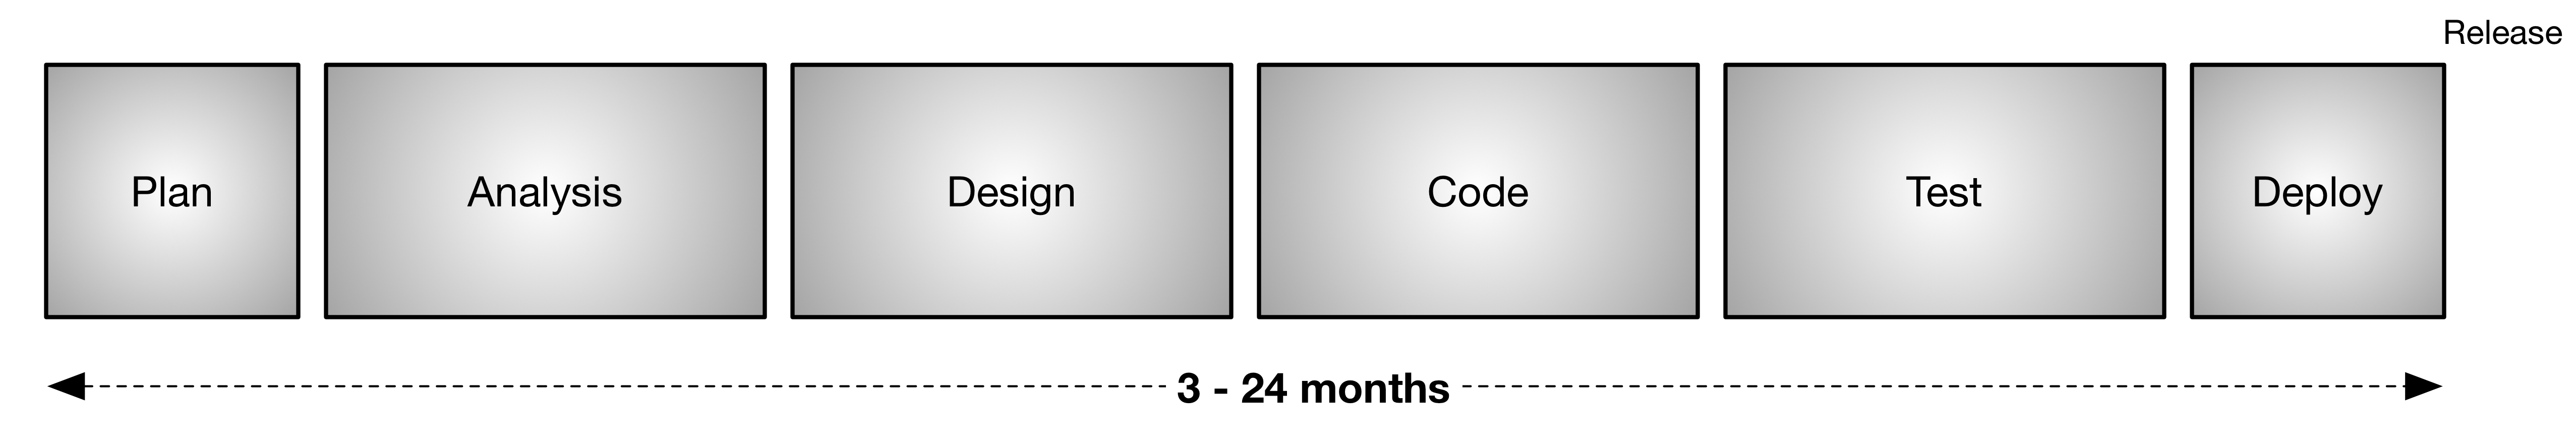
\includegraphics[width=0.95\linewidth]{images/waterfall}
  \caption{Phases of the water fall methodology.~\cite[p. 16]{shore-aad-2007}}
  \label{fig:waterfall}
\end{figure*}

\begin{figure*}[ht]
  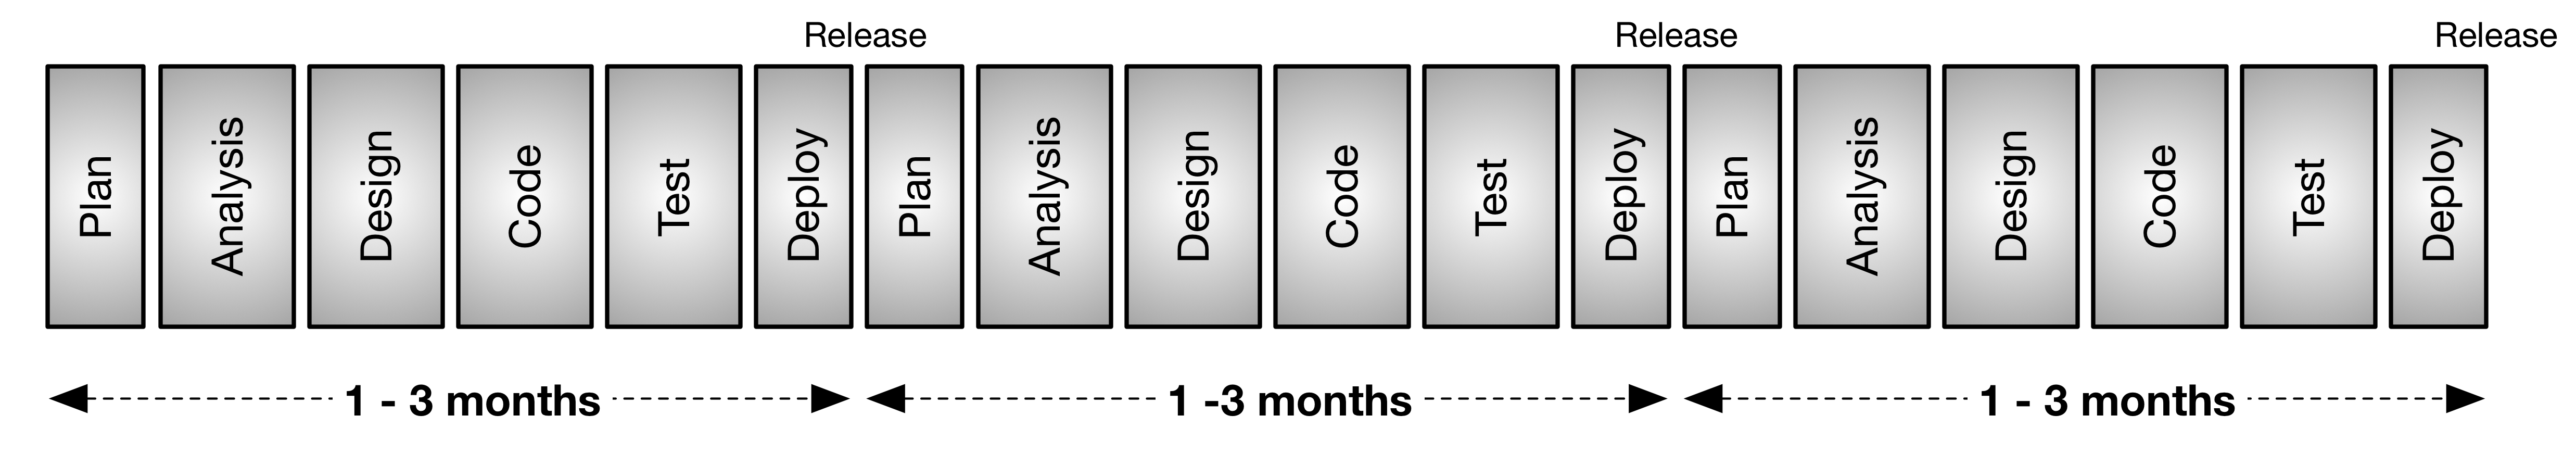
\includegraphics[width=0.95\linewidth]{images/iterative-dev}
  \caption{Phases of iterative development.~\cite[p. 16]{shore-aad-2007}}
  \label{fig:iterative-dev}
\end{figure*}

\newthought{By applying basic principles}, agile development methodologies try
to overcome this problem. These principles may vary depending on the used
methodology, but the fundamental principles are:
\begin{enumerate*}
  \item rapid feedback,
  \item assume simplicity,
  \item incremental change,
  \item embracing change and
  \item quality work.
\end{enumerate*}~\cite{beck-xp-2004}
Further details can be found at~\cite{beck-xp-2004, shore-aad-2007}.

\newthought{An adapted version of extreme programming} is used for this thesis.
This methodology was chosen as after the preceding project
work,~\citetitle{osterwalder-qde-2016}, several things were still subject to
change and therefore an exact planning, analysis and design, as traditional
methodologies require it, would not be very practical.
% TODO: Mention what exactly was modified.

\begin{figure*}[ht]
  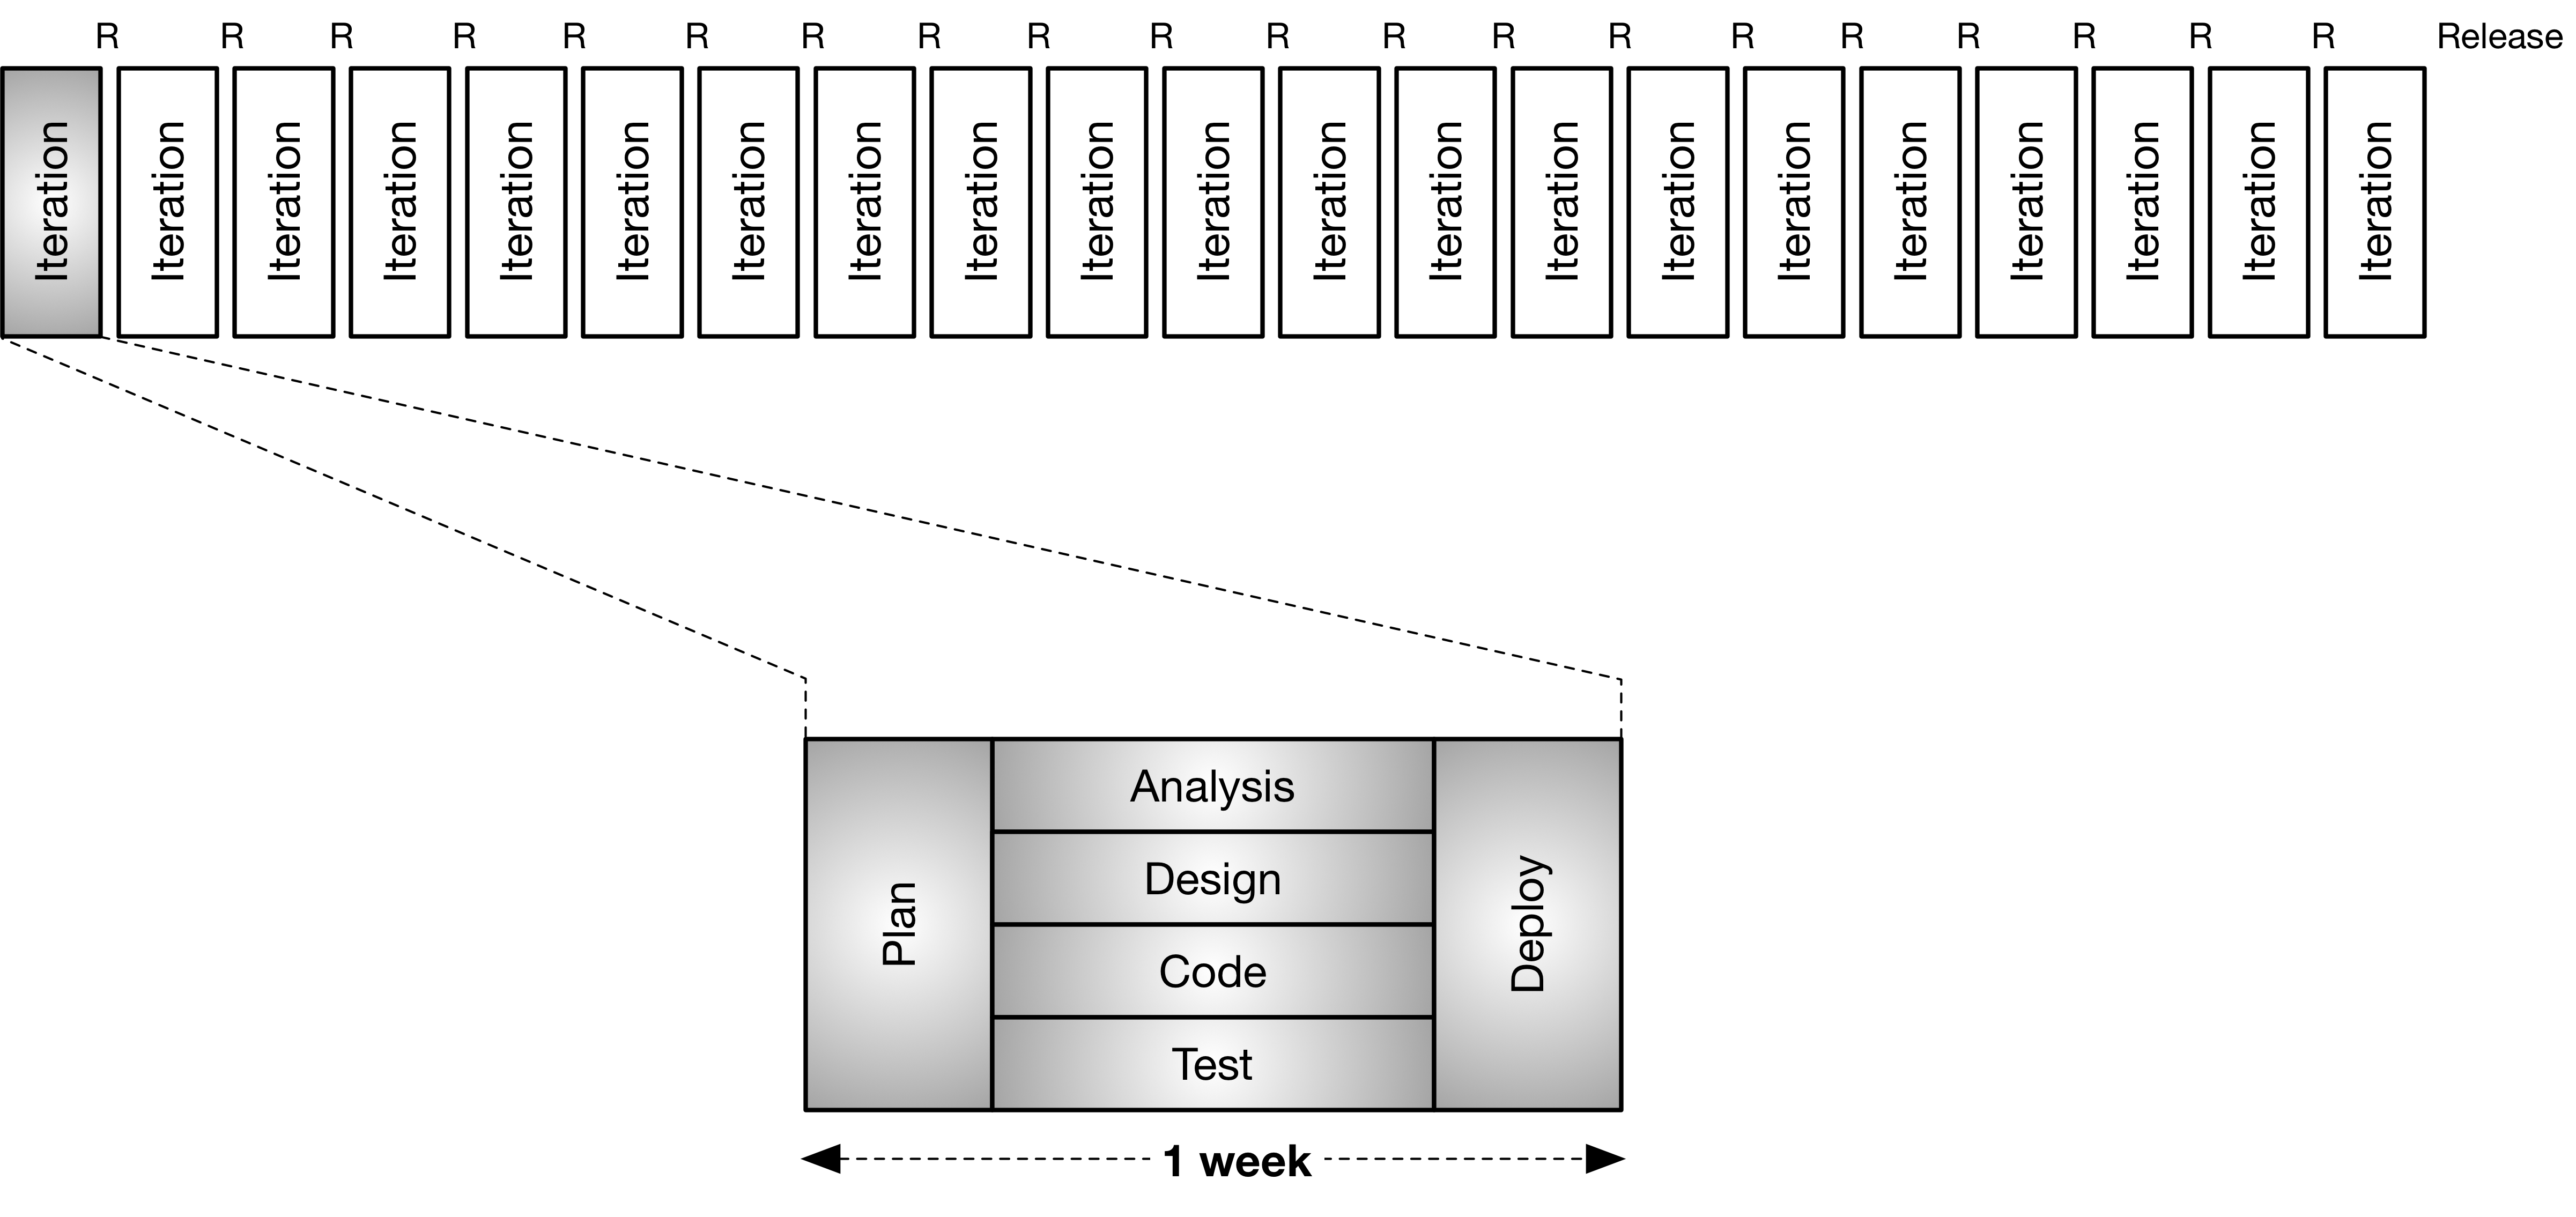
\includegraphics[width=0.95\linewidth]{images/xp}
  \caption{Iterations in the extreme programming methodology and phases of an
    interation.~\cite[p. 18]{shore-aad-2007}}
  \label{fig:xp}
\end{figure*}

% TODO: Check if this is enough or elaborate more otherwise.
% -*- mode: latex; coding: utf-8 -*-

\chapter{Implementation}
\label{chap:implementation}

% Gestützt auf Quellen, Messungen und Datenerhebungen werden die anhand der
% Fragestellung gewon- nenen Ergebnisse präsentiert [3, p. 116]. Während das
% Kapitel zu Material und Methoden ( 3.2.3) oder das entsprechende Unterkapitel
% der Einleitung die Versuchsanordnung beschreibt, werden im Kapitel Ergebnisse
% der Versuchsablauf mit den Resultaten objektiv wiedergegeben. Alle Überlegungen,
% Berechnungen oder Experimente des Berichts müssen vollständig nachvollziehbar
% sein [3, p. 26]. Zusammen mit der Diskussion und den Folgerungen machen die
% Ergebnisse qualitativ und quantitativ den Hauptteil des Berichts aus [3, p. 26].

% Link to previous
% Make a connection to what has immediately gone before. Recap the last chapter.
% In the last chapter I showed that… Having argued in the previous chapter that…
% As a result of x, which I established in the last chapter….. It is also possible
% to make a link between this chapter and the whole argument… The first step in
% answering my research question (repeat question) .. was to.. . In the last
% chapter I …
\newthought{The previous chapter} introduced the methodologies that are required
for understanding the results of this thesis.

% Focus: What does this chapter specifically do?
% Now focus the reader’s attention on what this chapter is specifically going to
% do and why it is important. In this chapter I will examine.. I will present… I
% will report … This is crucial in (aim of thesis/research question) in order to….
\newthought{This chapter} contours three sections. The first section shows the
software architecture that was developed and that is used for the program
implemented. Aspects of the literate form of this program implemented are shown
in the second section. The main concepts and the components of the program are
shown in the third section.

% Overview: How is it done?
% The third paragraph simply outlines the way that you are going to achieve the
% aim spelled out in the previous paragraph. It’s really just a statement of the
% contents in the order that the reader will encounter them. It is important to
% state these not simply as topics, but actually how they build up the internal
% chapter argument… I will begin by examining the definitions of, then move to
% seeing how these were applied… I first of all explain my orientation to the
% research process, positioning myself as a critical scholar.. I then explain the
% methodology that I used in the research, arguing that ethnography was the most
% suitable approach to provide answers to the question of…
% * Software architecture
% ** Reference to actual chapter
% ** Layers
% ** Signals
%
% * Literate programming
% ** Just mention, reference to actual chapter
%
% * Software
% ** Editor
% ** Player
% ** Components
%
% Nope, merged this already with focus.

% Input CF
% Resultate weniger kritisch, erst in Diskussion, überlappt sich aber.

\section{Software architecture}
\label{results:sec:software-architecture}

\newthought{The software architecture} defines the significant decisions of the
program implemented, such as the selection of structural elements, their
behavior and their interfaces.~\cite{kruchten_rup_2003} The architecture is
derived from the experiences based on the former
projects,~\citetitle{osterwalder-volume-2016}
and~\citetitle{osterwalder-qde-2016}, which build the fundamentals of this
thesis, see~\autoref{chap:fundamentals}~\enquote{\nameref{chap:fundamentals}}.

\newthought{Three aspects} define the software architecture:
\begin{enumerate}
  \item an architectural software design pattern,
  \item layers and
  \item signals and slots, which allow communication between components.
\end{enumerate}

\subsection{Software design}
\label{results:subsec:software-design}

\newthought{A [software] design pattern}~\enquote{names, abstracts, and
identifies the key aspects of a common design structure that make it useful for
creating a reusable object-oriented design. The design pattern identifies the
participating classes and instances, their roles and collaborations, and the
distribution of responsibilities. Each design pattern focuses on a particular
object-oriented design problem or issue.}~\cite[p. 16]{gamma-dpe-1995}

\newthought{To separate data from its representation} and to ensure a coherent
design, a combination of the model-view-controller (MVC)~\cite{krasner-mvc-1988}
and the model-view-view model pattern (MVVM)~\cite{fowler-presentation-2004,
gossman-mvvm-2005} is used as architectural software design pattern. This
decision is based on experiences from the previous projects and allows
individual parts to be modified and reused. This is especially necessary as the
data created in the editor component will be reused by the player component.

\newthought{Four kinds of components} build the basis of the pattern
used.~\Cref{table:software-design-pattern-components} provides a description of
the components.~\Cref{fig:software-design-pattern-components-editor} shows an
overview of the components of the editor (the colored items) including their
communication in an informal way. Additionally the user as well as the display
is shown (in gray color). As the player component only plays animations, no view
models are needed and therefore only the MVC pattern is used, which is shown
in~\cref{fig:software-design-pattern-components-player}.

\begin{table*}[h]
  \begin{tabularx}{\textwidth}{llX}
    \toprule
    \textbf{Component} & \textbf{Description} & \textbf{Examples} \\
    \midrule
    Model      & Represents the data or the business logic, & Scene, Node
                                                              Parameter\\
               & completely independent from the user       & \\
               & interface. It stores the state and does    & \\
               & the processing of the problem domain.      & \\
    \midrule
    View       & Consists of the visual elements.           & Scene tree view,
                                                              Scene view\\
    \midrule
    View model & \enquote{Model of a view}, the abstraction & Scene tree view
                                                              model, Scene\\
               & of the view, provides a specialization of  & view model, Node
                                                              view model\\
               & the model which the view can use for       & \\
               & data-binding. It also stores the state and & \\
               & may provide complex operations.            & \\
    \midrule
    Controller & Holds the data in terms of models.         & Scene tree
                                                              controller, scene
                                                              controller,\\
               & models. Acts as an interface between the   & node controller\\
               & components.                                & \\
    \bottomrule
  \end{tabularx}
  \caption{Description of the types of components of the software design
    pattern used.~\cite{fowler-presentation-2004, gossman-mvvm-2005}}
  \label{table:software-design-pattern-components}
\end{table*}

\begin{figure*}[ht]
  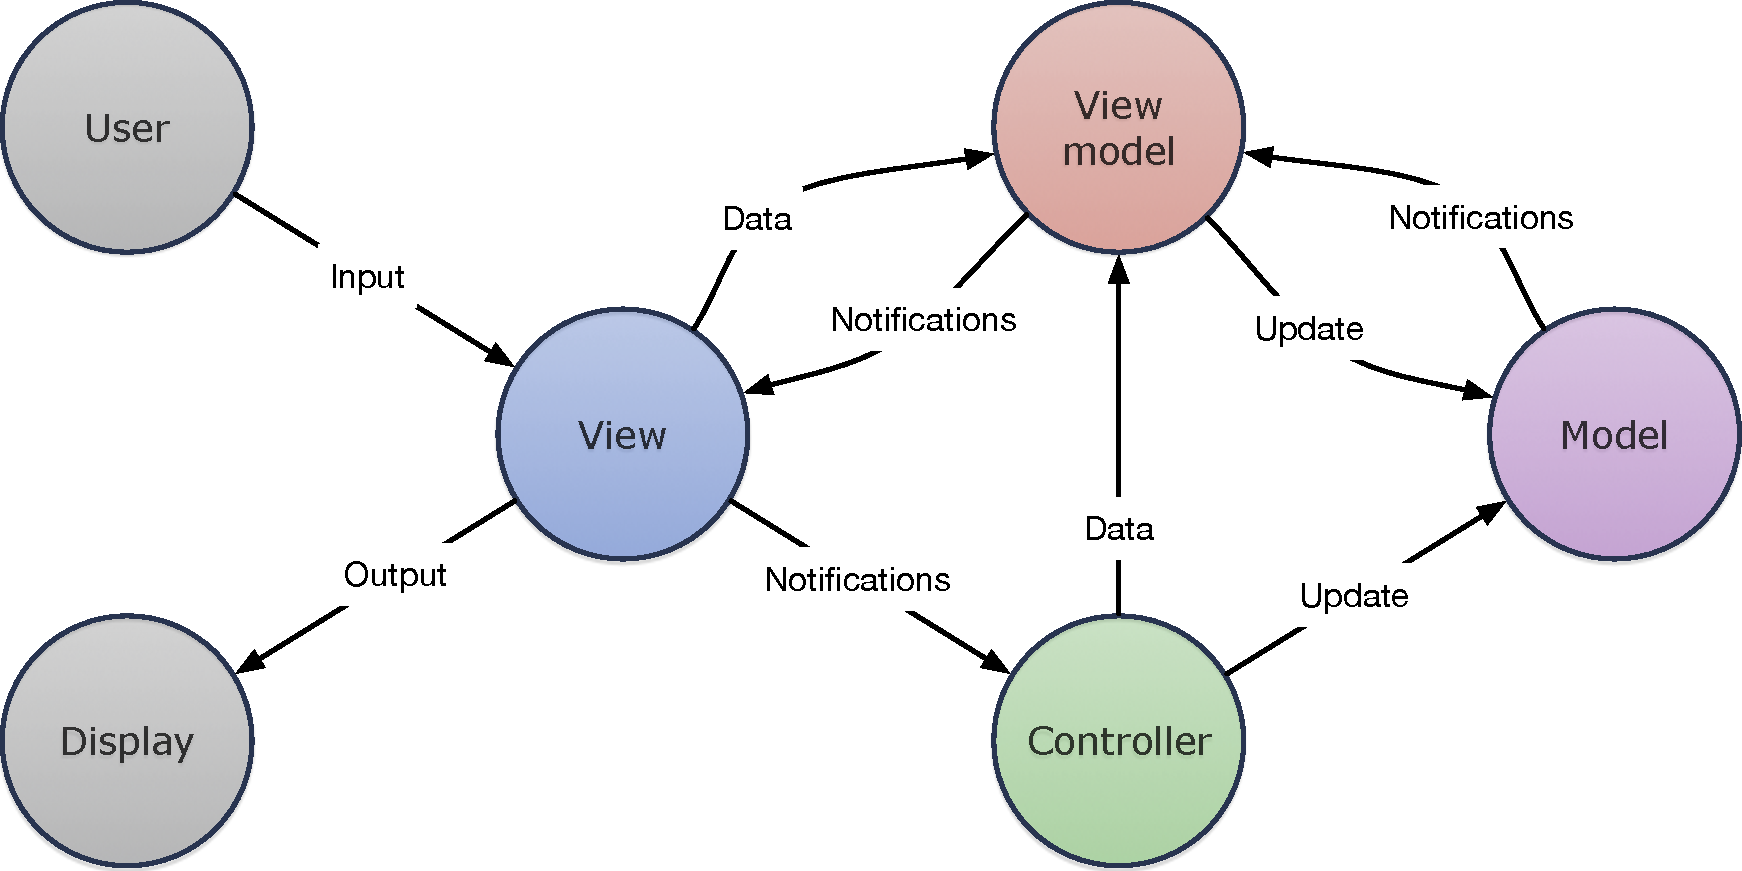
\includegraphics[width=0.8\linewidth]{images/mvvmc}
  \caption{Components of the used pattern for the editor and their
    communication.}
  \label{fig:software-design-pattern-components-editor}
\end{figure*}

\begin{figure*}[ht]
  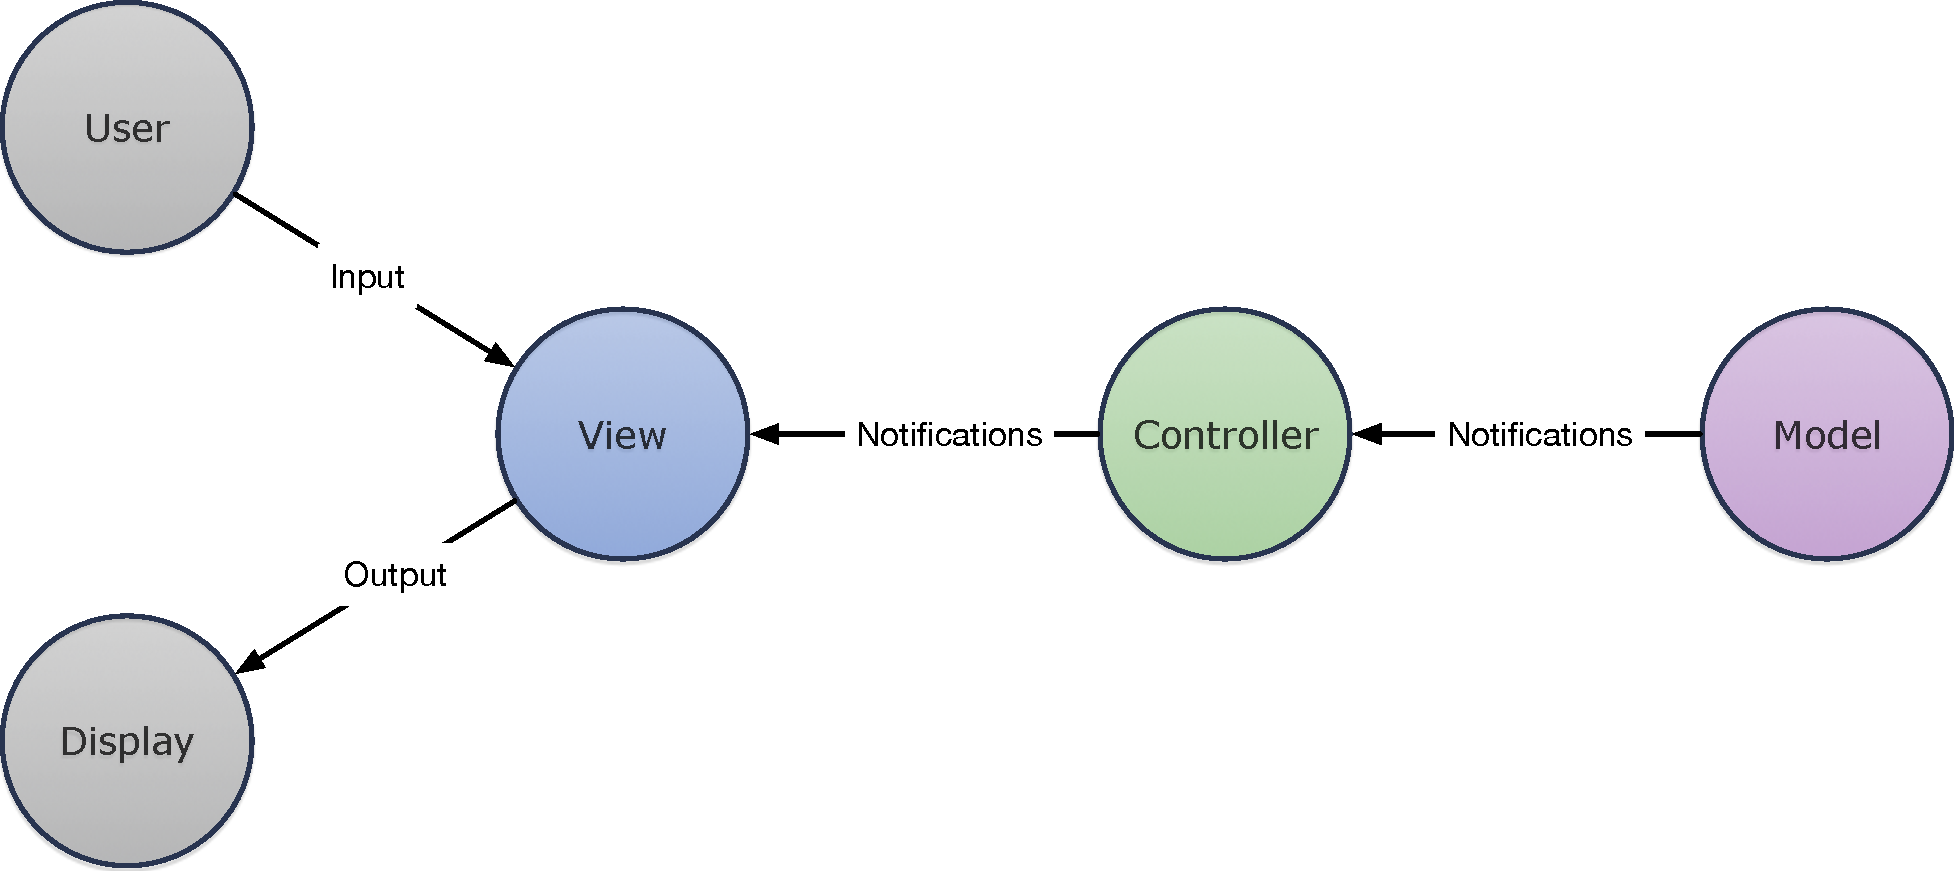
\includegraphics[width=0.8\linewidth]{images/mvvmc-player}
  \caption{Components of the used pattern for the player and their
    communication.}
  \label{fig:software-design-pattern-components-player}
\end{figure*}

\newthought{The Qt framework} which is used, offers a very similar pattern
called~\enquote{model/view pattern}. It combines the view and the controller
into a single object. The pattern introduces a delegate between view and model,
similar to a view model. The delegate allows editing the model and communicates
with the view. The communication is done by so called model indexes, which are
references to items of data.~\cite{qt-mvp-2017}~\enquote{By supplying model
indexes to the model, the view can retrieve items of data from the data source.
In standard views, a delegate renders the items of data. When an item is edited,
the delegate communicates with the model directly using model
indexes.}~\cite{qt-mvp-2017} \Cref{fig:software-design-pattern-qt-mvp} shows
this model/view pattern.

\begin{figure}[ht]
  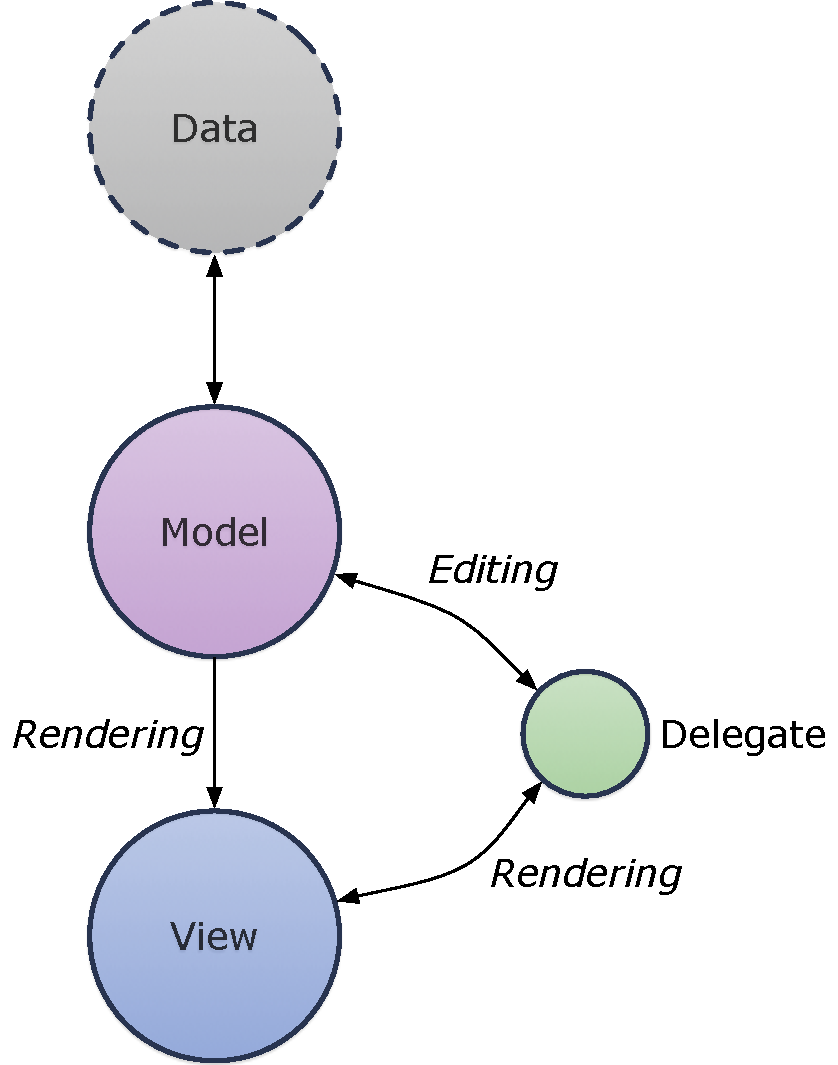
\includegraphics[width=0.6\linewidth]{images/model-view-pattern}
  \caption{Qt's model/view pattern.~\cite{qt-mvp-2017}}
  \label{fig:software-design-pattern-qt-mvp}
\end{figure}

\newthought{Although offering advantages}, such as to customize the presentation
of items or the usage of a wide range of data sources, the model/view pattern was
not used in this project. This is mainly due to two reasons:
\begin{enumerate*}
  \item the developed and intended components use no data source other than external
    files and
  \item the concept of using model indexes may add flexibility but also
    introduces overhead.
\end{enumerate*}

\newthought{The scene tree component} of the editor was developed using the Qt
class for the abstract item model, which uses the model/view pattern. This
showed that the usage of this pattern introduces unnecessary overhead and
requires more effort to implement, while not using the advantages of features of
the pattern. Therefore a decision was taken against the usage of the pattern in
this case.

\subsection{Layers}
\label{results:subsec:layers}

\newthought{To reduce coupling and dependencies} a relaxed layered architecture
is used, as written
in~\autoref{results:sec:software-architecture}~\enquote{\nameref{results:sec:software-architecture}}.
In contrast to a strict layered architecture, which allows any layer to call
only services or interfaces from the layer below, the relaxed layered
architecture allows higher layers to communicate with any lower
layer.~\Cref{table:results:layers} provides a graphical overview as well as a
description of the layers. The colors have no significance except to distinguish
the layers visually for the reader.

\begin{table*}[h]
  \begin{tabularx}{\textwidth}{XXX}
    \toprule
    \textbf{Layer} & \textbf{Description} & \textbf{Examples} \\
    \midrule
    
\includegraphics[width=0.9\linewidth]{images/layers-gui}         & All elements of the graphical user interface, views.                                & Scene tree view, scene view, render view                                   \\
    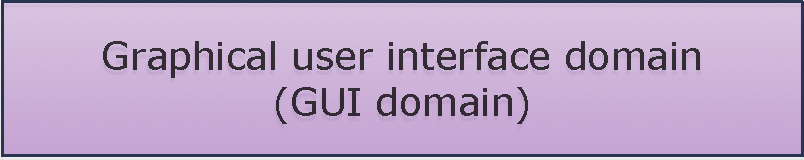
\includegraphics[width=1.0\linewidth]{images/layers-gui-domain}  & View models.                                                                        & Scene tree view model, node view model                                     \\
    
\includegraphics[width=1.0\linewidth]{images/layers-application} & Controller (workflow objects).                                                      & Main application, scene tree controller, scene controller, node controller \\
    
\includegraphics[width=1.0\linewidth]{images/layers-domain}      & Data models according to the logic of the application.                              & Scene model, parameter model, node definition model, node domain model     \\
    
\includegraphics[width=1.0\linewidth]{images/layers-technical}   & Technical infrastructure, such as graphics, window creation and so on.              & JSON parser, camera, culling, graphics, renderer                           \\
    
\includegraphics[width=1.0\linewidth]{images/layers-foundation}  & Basic elements and low level services, such as timer, arrays or other data classes. & Colors, common, constants, flags                                           \\
    \bottomrule
  \end{tabularx}
  \vspace*{\baselineskip}
  \caption{Layers of the program implemented.}
  \label{table:results:layers}
\end{table*}

\subsection{Coupling and cohesion, signals and slots}
\label{results:subsec:signals}

% Signals:  Explain what signals are and how they are used, maybe draw an
% illustrative diagram.

\newthought{Whenever designing and developing} software, coupling and cohesion
can occur and may pose a problem if not considered early and well enough.

\newthought{Coupling} measures how strongly a component is connected to other
components, or has knowledge of them or depends on them. High coupling impedes
the readability and maintainability of software, so programmers should strive
towards low coupling. \citeauthorfin{larman-applying-2004} states that the
principle of low coupling applies to many dimensions of software development and
that it is a major objective in building software.~\cite{larman-applying-2004}

\newthought{Cohesion} is a measurement of~\enquote{how functionally related the
operations of a software element are, and also measures how much work a software
element is doing}.~\cite{larman-applying-2004} Or put otherwise, it
is~\enquote{a measure of the strength of association of the elements within a
module}.~\cite[p. 52]{ieee-swebok-2014} Low (or poor) cohesion does not imply
that a component works only by itself, indeed it probably collaborates with many
other objects. But low cohesion tends to create high (poor) coupling. It is
therefore desirable to keep objects focused, understandable and manageable while
supporting low coupling.~\cite{larman-applying-2004}

\newthought{To overcome the problems} of high coupling and low
cohesion,~\emph{signals and slots} are used. Signals and slots are a generalized
implementation of the observer pattern, which can be seen informally
in~\cref{fig:signals-observer-pattern}
and~\cref{fig:signal-and-slot-relationship}.

\begin{figure}[ht]
  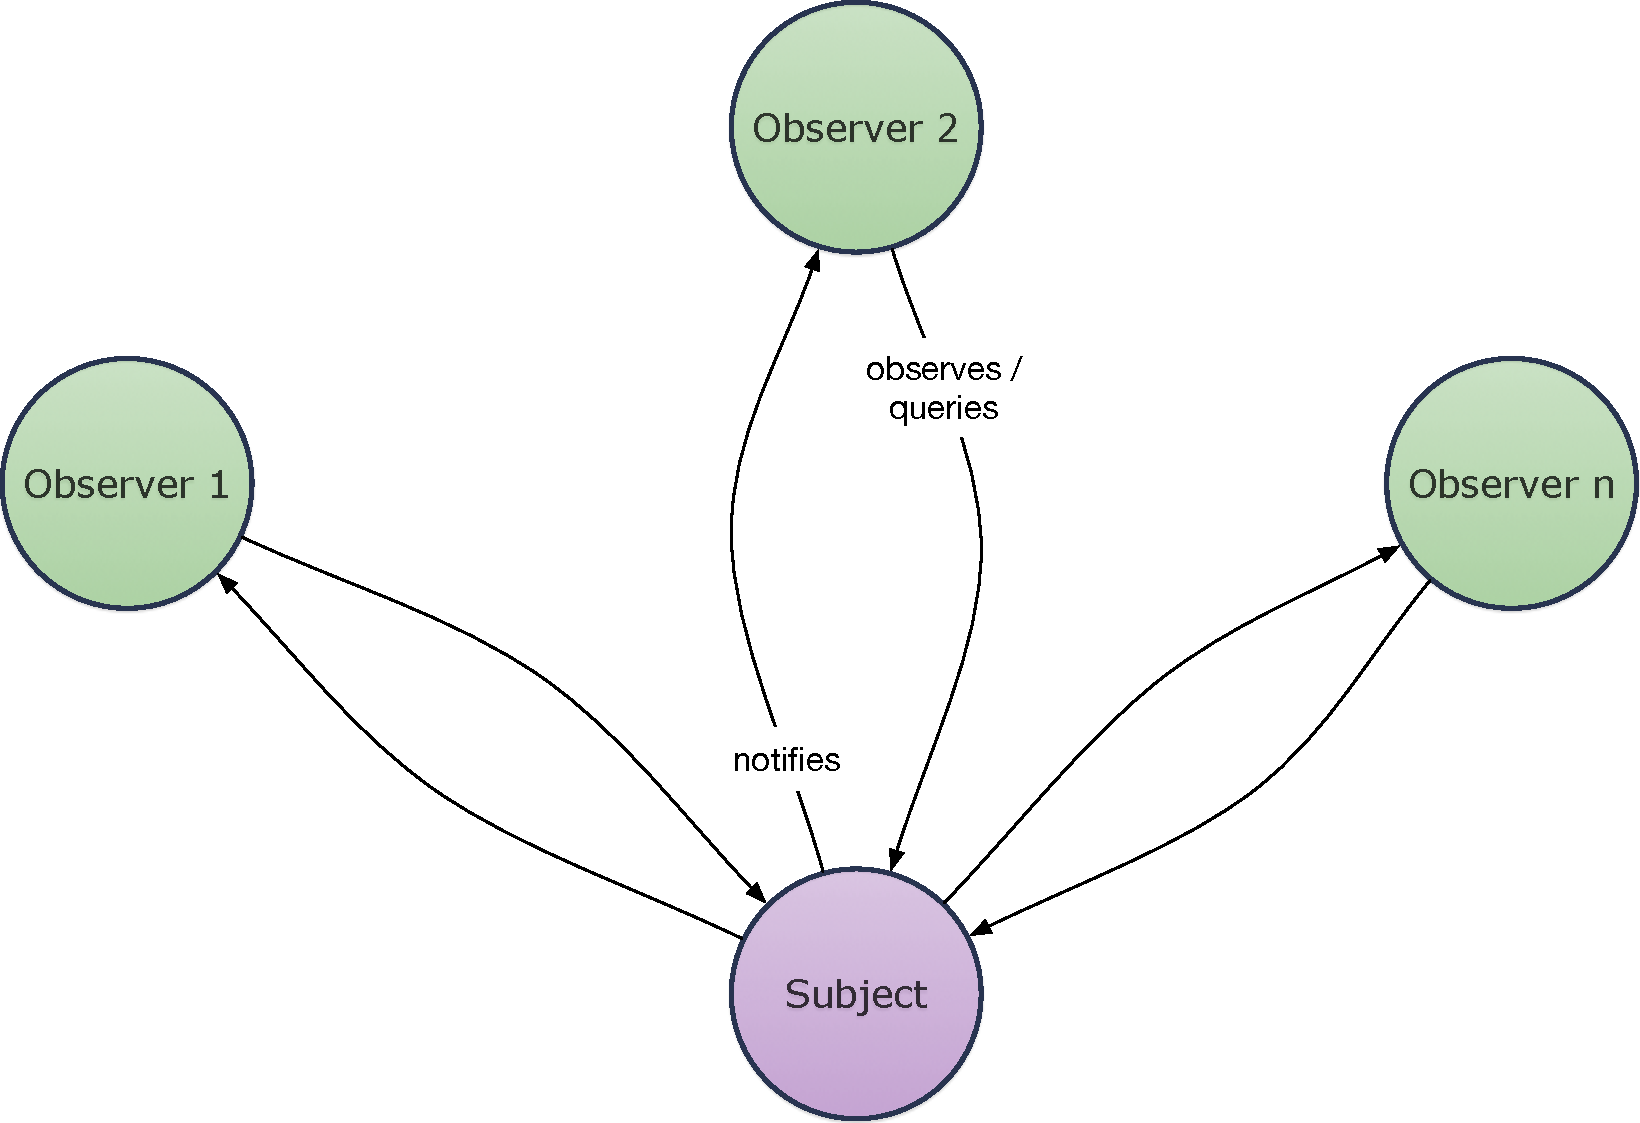
\includegraphics[width=0.8\linewidth]{images/observer-pattern}
  \caption{The observer pattern.~\cite{gamma-dpe-1995}}
  \label{fig:signals-observer-pattern}
\end{figure}

\newthought{A signal is an observable event.} A slot is a potential observer,
typically a method of an object.

\begin{figure}
  \begin{pythoncode}
class Observer:

    @slot(type)
    def on_signal(self, parameter):
        """Listens on the signal 'signal'. Expects the
        signal to send the parameter 'parameter' of
        type 'type'."""
      
        ...
  \end{pythoncode}
  \label{lst:signal-slot:observer-slot}
  \caption{An example of a class called~\enquote{Observer} with a slot
    called~\enquote{on\_signal}. The slot expects the signal to send a parameter
    of type~\enquote{type}.
  }
\end{figure}

\newthought{Slots are registered as observers} to signals.

\begin{figure}
  \begin{pythoncode}
subject.signal.connect(
    observer.on_signal
)
  \end{pythoncode}
  \label{lst:signal-slot:connect}
  \caption{The~\enquote{on\_signal} slot (which is a method of the
    object~\enquote{observer}) is registered to the signal~\enquote{signal} of
    the object~\enquote{subject}.}
\end{figure}

\newthought{Whenever a signal is emitted}, the emitting class must call all the
registered observers for that signal.

\begin{figure}
  \begin{pythoncode}
subject.signal.emit(some_parameter)
  \end{pythoncode}
  \label{lst:signal-slot:emit}
  \caption{The signal~\enquote{signal} of the object~\enquote{subject} is
    emitted. The signal contains a parameter called~\enquote{some\_parameter}.
    This means that the emitting class,~\enquote{Signal}, will call the
    registered method~\enquote{on\_signal} of the observer
    called~\enquote{observer}.}
\end{figure}

\newthought{The relationship between signals and slots} is a many-to-many
relationship. One signal may be connected to any number of slots and a slot may
listen to any number of signals. A relationship between a signal and a slot is
shown in~\cref{fig:signal-and-slot-relationship}

\begin{figure}[ht]
  
\includegraphics[width=0.8\linewidth]{images/signal-and-slot}
  \caption{An observer is listening to a signal sent by a subject. The subject
    emits the signal and calls then the observers that are registered for that
    signal (or the registered slots of the observers respectively).}
  \label{fig:signal-and-slot-relationship}
\end{figure}

\newthought{Signals can carry additional information}, such as single values or
even references to objects. A simple example of a signal-slot relationship is
loading node definitions from files. The node controller, when it loads node
definitions, could emit two signals to inform other components. For example,
signal 1
\begin{enumerate*}
  \item gives the number of node definitions to load, and signal
  \item the index of the last loaded node definition and a reference to it.
\end{enumerate*}
This information could for example be used in a dialog showing the progress of
loading from the file system.

\begin{figure}
  \begin{pythoncode}
self.total_node_definitions.emit(num_node_definitions)
  \end{pythoncode}
  \label{lst:signal-slot-example-1}
  \caption{%
    An example of emitting a signal including a value.
  }
\end{figure}

\begin{figure*}
  \begin{pythoncode}
for index, definition_file in enumerate(node_definition_files):
    node_definition = self.load_node_definition_from_file(
        definition_file
    )
    self.node_definition_loaded(index, node_definition)
  \end{pythoncode}
  \label{lst:signal-slot-example-2}
  \caption{%
    An example of emitting a signal including a value and a reference to an
    object.
  }
\end{figure*}

\section{Literate programming}
\label{results:sec:literate-programming}

\newthought{Documentation is crucial to the maintenance or modification} of any
software project. However, all too frequently the documentation is not done
properly or is even neglected because of seemingly low benefit related to
effort. No documentation at all, outdated or irrelevant documentation can cause
unforeseen cost and time overruns. Using the literate programming paradigm
prevents these problems, as the software as well as the documentation are
derived from a literate program. For this thesis the LP system nuweb was used,
as described
under~\autoref{sec:literate-programming}~\enquote{\nameref{sec:literate-programming}}.

\newthought{Using literate programming to develop software} requires a different
way of thinking from traditional methodologies. The approach is completely
different. Traditional methodologies focus on instructing the computer what to
do by writing program code. Literate programming focuses on explaining to human
beings what the computer shall do by combining the documentation with code in a
single document. From this single document a program which can be compiled or
run directly is extracted. The order of the code fragments matters only
indirectly, they may appear in any order throughout the text. The code fragments
are put into the right order for compilation or running by defining the output
files containing the needed code fragments in the right order.

\newthought{The need to include every detail} makes literate programming very
expressive and verbose. While this expressiveness may be an advantage for small
software and partly also for larger software, it can also be a problem,
especially for larger software: the documentation becomes lengthy and hard to
read, especially when including the full implementation of technical details.

\newthought{These problems} in the writing of this thesis were overcome by
moving the implementation into the appendix,
see~\autoref{part:appendix}~\enquote{\nameref{part:appendix}} and by outsourcing
technical parts into a separate file,
see~\autoref{sec:code-fragments}~\enquote{\nameref{sec:code-fragments}}.

\section{Program}
\label{results:sec:program}

\newthought{To recall}, the objective of this thesis is the design and
development of a program for modeling, composing and rendering real-time
computer graphics by providing a graphical toolbox.

\newthought{Using the introduced methodologies}
(see~\autoref{chap:methodologies}~\enquote{\nameref{chap:methodologies}}) and
the developed software architecture
(see~\autoref{results:sec:software-architecture}~\enquote{\nameref{results:sec:software-architecture}})
a program was implemented.

\newthought{The program implemented} should to have two main components:
the~\textit{editor} and~\textit{player}.

\newthought{The editor component} provides a graphical system for modeling,
composing and rendering of scenes. It allows composing scenes into an animation
and saving the animation in an external file. Rendering is done using the shown
sphere tracing algorithm combined with Phong shading.

\newthought{The player component} simply plays an animation which has been
created with the editor component. This includes loading and rendering of all
scenes.

\newthought{Due to time constraints}, however, only the editor component was
implemented.~\autoref{fig:editor} shows an image of the program implemented.

\newthought{For the implementation} the following tools were used: the Python
programming language~\protect\footnote{version 3.5.2,
\url{http://www.python.org}}, the Qt cross-platform application development
framework~\protect\footnote{version 5.7, \url{https://www.qt.io/}}, the PyQt5
bindings~\protect\footnote{version 5.7,
\url{https://riverbankcomputing.com/software/pyqt/intro}} for Qt and
OpenGL~\protect\footnote{version 3.3, \url{https://www.opengl.org/}}.

\begin{figure}[ht]
  \caption{The implemented editor component.}
  \label{fig:editor}
  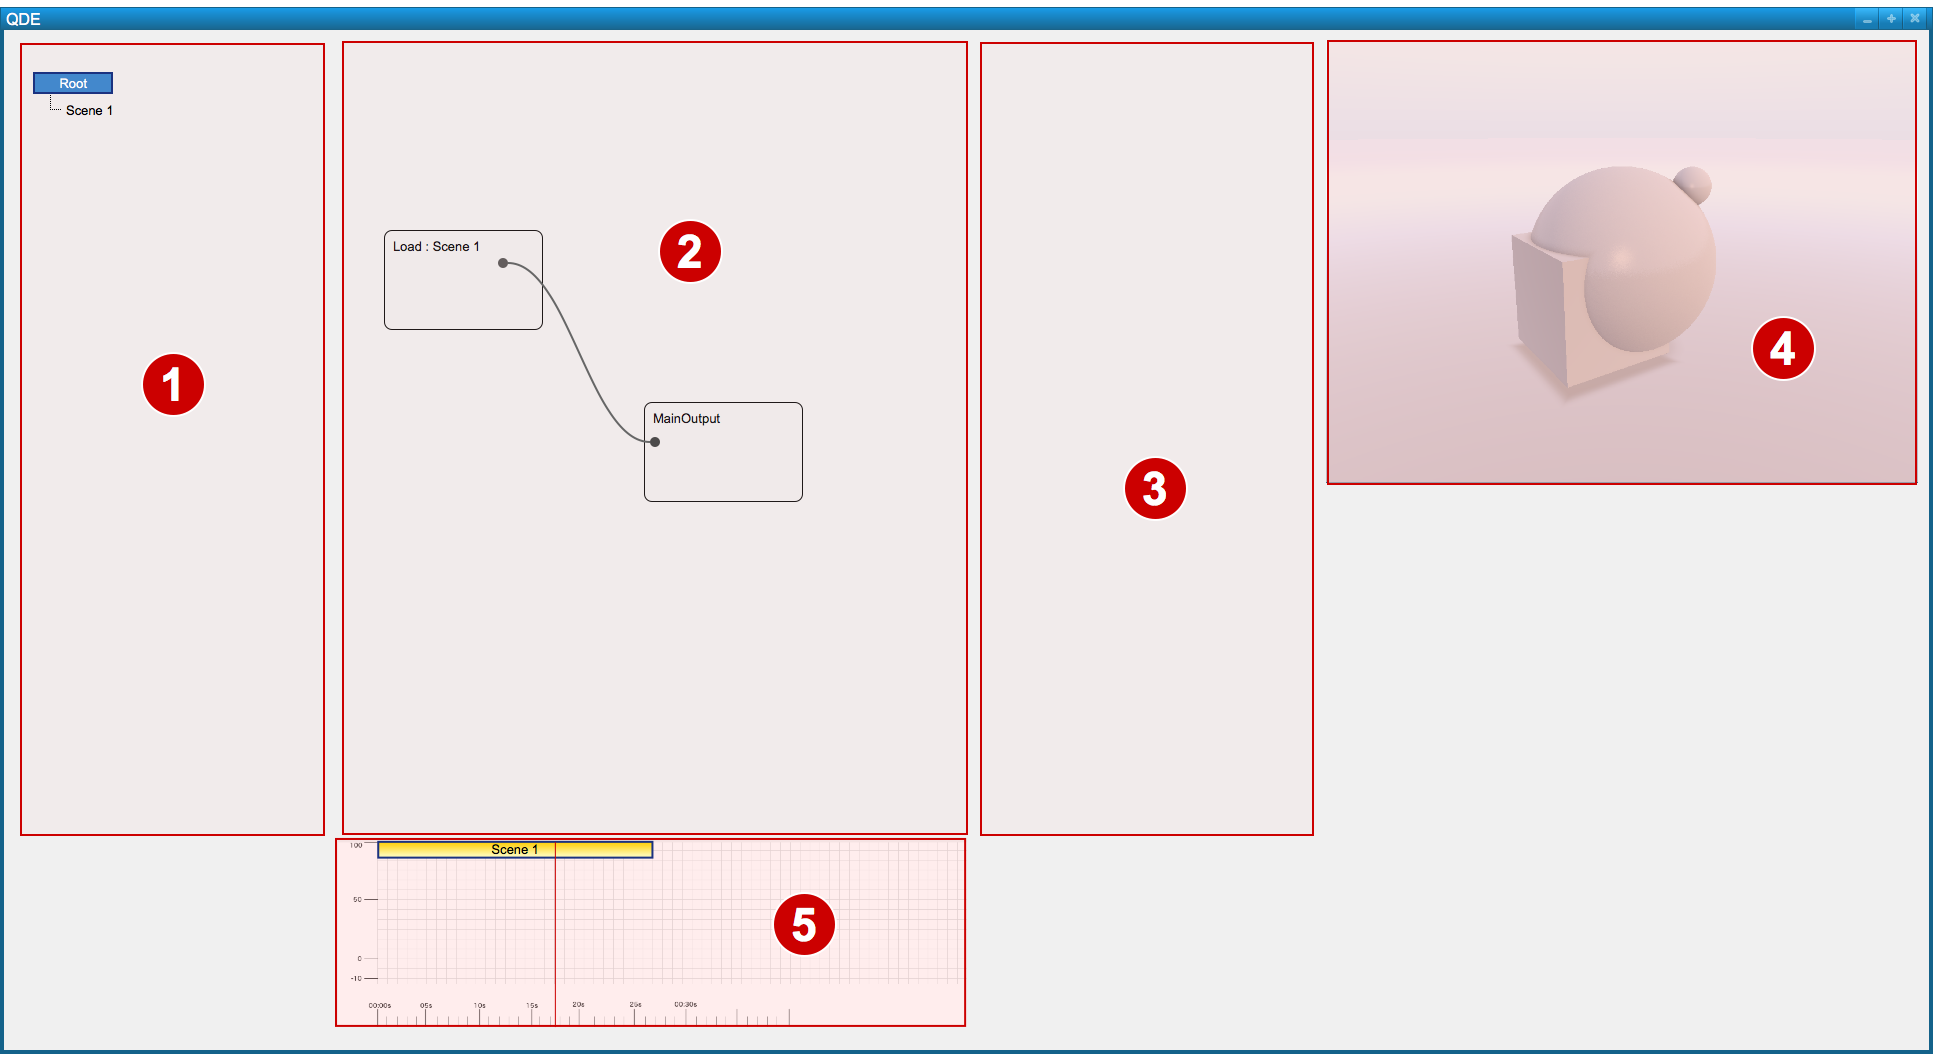
\includegraphics[width=0.95\linewidth]{images/editor-components}
\end{figure}
\todo[inline]{Provide real image of the component, but use numbering for the
  components.}

\newthought{The quintessence of both components} is to output respectively to
read a data structure in the JSON~\cite{ecma-json-2013} format which defines an
animation. This data structure provides an animation which contains scenes,
which contain nodes. This data structure is evaluated and the result is
shader-specific code which is executed by the graphical processing unit (GPU)
and seen by the viewer.

\newthought{An animation} is simply a composition of scenes which run in a
sequential order within a defined time span.

\newthought{A scene} is a composition of nodes stored in the form of a directed
graph.

\newthought{Nodes} are instances of node definitions and define the content of a
scene and therefore of an animation.

\newthought{Node definitions} provide content in a specific structure, shown
in~\autoref{table:node-definition-components}.

\begin{table}\centering
  \ra{1.3}
  \begin{tabularx}{\textwidth}{@{}lX@{}}
    \toprule
    \textbf{Property}    & \textbf{Description}                                \\
    \hline
    \textit{ID}          & A global unique identifier.                         \\
    \textit{Name}        & The name of the node, e.g. "Sphere".                \\
    \textit{Description} & A description of the node's purpose.                \\
    \textit{Inputs}      & Parameters given to the node. These may have 
    distinct types, e.g. scalars as floating point numbers or character strings
    of type text, references to other nodes.                                   \\
    \textit{Outputs}     & Values delivered by the node.                       \\
    \textit{Definitions} & A list of the node's definitions. This may be an
    actual definition of a (shader-) function in terms of an implicit surface. \\
    \textit{Invocation}  & The format of a call to the node definition, including
    placeholders which will be replaced by parameters.                         \\
    \textit{Parts}       & Defines text that may be processed when calling the node.
    Contains code which can be interpreted directly.                           \\
    \textit{Nodes}       & The children a node has (child nodes). These entries are
    references to other nodes only.                                            \\
    \textit{Parameters}  & A list of the node's inputs and outputs in form of
    tuples.
    Each tuple is composed of two parts:~\begin{enumerate*}
      \item a reference to another node and
      \item a reference to an input parameter or an output value of that node.
    \end{enumerate*} If the first reference is not set, this means that the
    parameter is internal.                                                     \\
    \bottomrule
  \end{tabularx}
  \caption{Properties/attributes of a node definition.}
  \label{table:node-definition-components}
\end{table}

\newthought{Content} is whatever a node definition provides in terms of the
definitions but the output has always to be an atomic type as defined
in~\autoref{table:node-definition-atomic-types}.

\begin{table}\centering
  \ra{1.3}
  \begin{tabularx}{\textwidth}{@{}lX@{}}
    \toprule
    \textbf{Atomic type} & \textbf{Description}                                         \\
    \hline
    \textit{Generic}     & A global unique identifier (UUID\protect\footnotemark[1]{}). \\
    \textit{Float}       & The name of the node, e.g. "Sphere".                         \\
    \textit{Text}        & A description of the node's purpose.                         \\
    \textit{Scene}       & Parameters given to the node as inputs. This may be          \\
    \textit{Image}       & Values delivered by the node as outputs.                     \\
    \textit{Dynamic}     & A list of the node's definitions. This may be an             \\
    \textit{Mesh}        & The format of a call to the node definition, including       \\
    \textit{Implicit}    & Defines text that may be processed when calling the node.    \\
    \bottomrule
  \end{tabularx}
  \caption{Atomic types, that define a node (definition).}
  \label{lst:node-definition-atomic-types}
\end{table}

\newthought{An example} of an node definition of type~\emph{implicit} for
rendering a sphere is given in~\autoref{fig:implicit-sphere-node-definition}.
\begin{figure*}
  \begin{minted}[%
    bgcolor=LightGray,
    escapeinside=||,
    linenos=true,
    mathescape=true,
    tabsize=4]{js}
{
    "name": "Implicit sphere",
    "id_": "16d90b34-a728-4caa-b07d-a3244ecc87e3",
    "description": "Definition of a sphere by using implicit surfaces",
    "inputs": [
        
{
    "name": "radius",
    "atomic_id": "468aea9e-0a03-4e63-b6b4-8a7a76775a1a",
    "default_value": {
        "type_": "float",
        "value": "1"
    },
    "id_": "f5c6a538-1dbc-4add-a15d-ddc4a5e553da",
    "description": "The radius of the sphere",
    "min_value": "-1000",
    "max_value": "1000"
}
    ],
    "outputs": [
        
{
    "name": "output",
    "id_": "a3ac68e5-5afe-4779-9e9f-5b619e041ae6",
    "atomic_id": "c019271c-35b6-425c-9ff2-a1d893111adb"
}
    ],
    "definitions": [
        
{
    "id_": "99d20a26-f233-4310-adb2-5e540726d079",
    "script": [
        "// Returns the signed distance to a sphere with given radius for the",
        "// given position.",
        "float sphere(vec3 position, float radius)",
        "{",
        "    return length(position) - radius;",
        "}"
    ]
}
    ],
  \end{minted}
  \label{fig:node-definition-atomic-type}
  \caption{Teh cap.}
\end{figure*}

\begin{figure*}
  \begin{minted}[%
    bgcolor=LightGray,
    escapeinside=||,
    linenos=true,
    mathescape=true,
    tabsize=4]{js}
    "invocations": [
        
{
    "id_": "4cd369d2-c245-49d8-9388-6b9387af8376",
    "type": "implicit",
    "script": [
        "float s = sphere(",
        "    16d90b34-a728-4caa-b07d-a3244ecc87e3-position,",
        "    5c6a538-1dbc-4add-a15d-ddc4a5e553da",
        ");"
    ]
}
    ],
    "parts": [
        
{
    "id_": "74b73ce7-8c9d-4202-a533-c77aba9035a6",
    "name": "Implicit sphere node function",
    "type_": "implicit",
    "script": [
        "# -*- coding: utf-8 -*-",
        "",
        "from PyQt5 import QtGui",
        "",
        "",
        "class Class_ImplicitSphere(object):",
        "    def __init__(self):",
        "        self.position = QtGui.QVector3D()",
        "",
        "    def process(self, context, inputs):",
        "        shader = context.current_shader.program",
        "        ",
        "        radius = inputs[0].process(context).value",
        "        shader_radius_location = shader.uniformLocation(\"f5c6a538-1dbc-4add-a15d-ddc4a5e553da\")",
        "        shader.setUniformValue(shader_radius_location, radius)",
        "        ",
        "        position = self.position",
        "        shader_position_location = shader.uniformLocation(",
        "            \"16d90b34-a728-4caa-b07d-a3244ecc87e3-position\"",
        "        )",
        "        shader.setUniformValue(shader_position_location, position)",
        "        ",
        "        return context"
    ]
}
    ],
  \end{minted}
  \label{fig:node-definition-atomic-type-2}
  \caption{Teh cap 2.}
\end{figure*}

\begin{figure*}
  \begin{minted}[%
    bgcolor=LightGray,
    escapeinside=||,
    linenos=true,
    mathescape=true,
    tabsize=4]{js}
    "nodes": [
        
    ],
    "connections": [
        
{
    "source_node": "00000000-0000-0000-0000-000000000000",
    "source_part": "f5c6a538-1dbc-4add-a15d-ddc4a5e553da",
    "target_node": "00000000-0000-0000-0000-000000000000",
    "target_part": "74b73ce7-8c9d-4202-a533-c77aba9035a6"
}
    ]
}
  \end{minted}
  \label{fig:node-definition-atomic-type-3}
  \caption{Teh cap 3.}
\end{figure*}

\newthought{Subsequent each component of the editor} is shown in a component
diagram in adapted form \cite[pp. 653 -- 654]{larman-applying-2004} and an
entity relationship diagram~\cite[pp. 501 ff.]{larman-applying-2004} (if
appropriate), followed by a description of the component. The component diagram
is used to show the signals that a component emits and receives. The entity
relationship diagram is used to show the relationships between components. Only
the relations immediately related to the presented component are shown, because
the diagrams would otherwise be too crowded and confusing.

\newthought{To preserve clarity} all components are described in discrete
sections of this chapter. Although the implementation of the components is very
specific, in terms of the programming language, their logic may be reused later
for the player component.

\subsection{Editor}
\label{results:subsec:program:editor}

\begin{figure*}[ht]
  \caption{Component diagram of the editor component.}
  \label{fig:editor-component-diagram}
  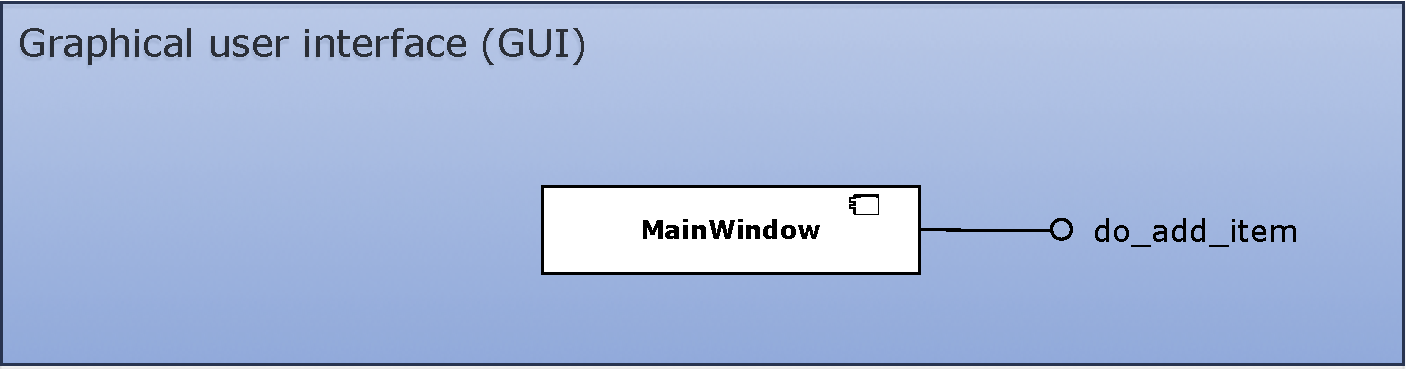
\includegraphics[width=0.95\linewidth]{images/editor-component-diagram}
\end{figure*}

\begin{figure}[ht]
  \caption{Entity relationship diagram of the editor component.}
  \label{fig:editor-erd}
  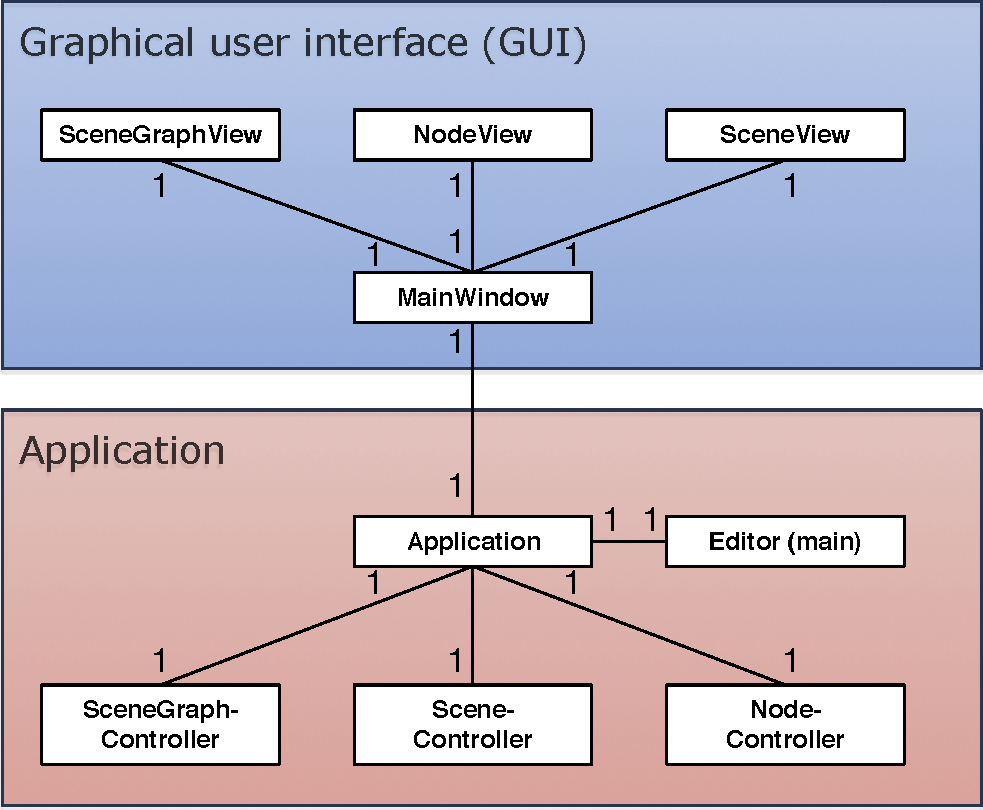
\includegraphics[width=0.75\linewidth]{images/editor-erd}
\end{figure}

\newthought{The editor component} is the main component, which acts as entry
point for the application and ties all components together.
The~\verb=Application= class sets up all the controllers and the main window.
The~\verb=MainWindow= class sets up all the view-related components, therefore
the scene tree view, the scene view and the renderer.

\subsection{Scene tree}
\label{results:subsec:program:scene-tree}

\begin{figure*}[ht]
  \caption{Component diagram of the scene tree component.}
  \label{fig:scene-graph-component-diagram}
  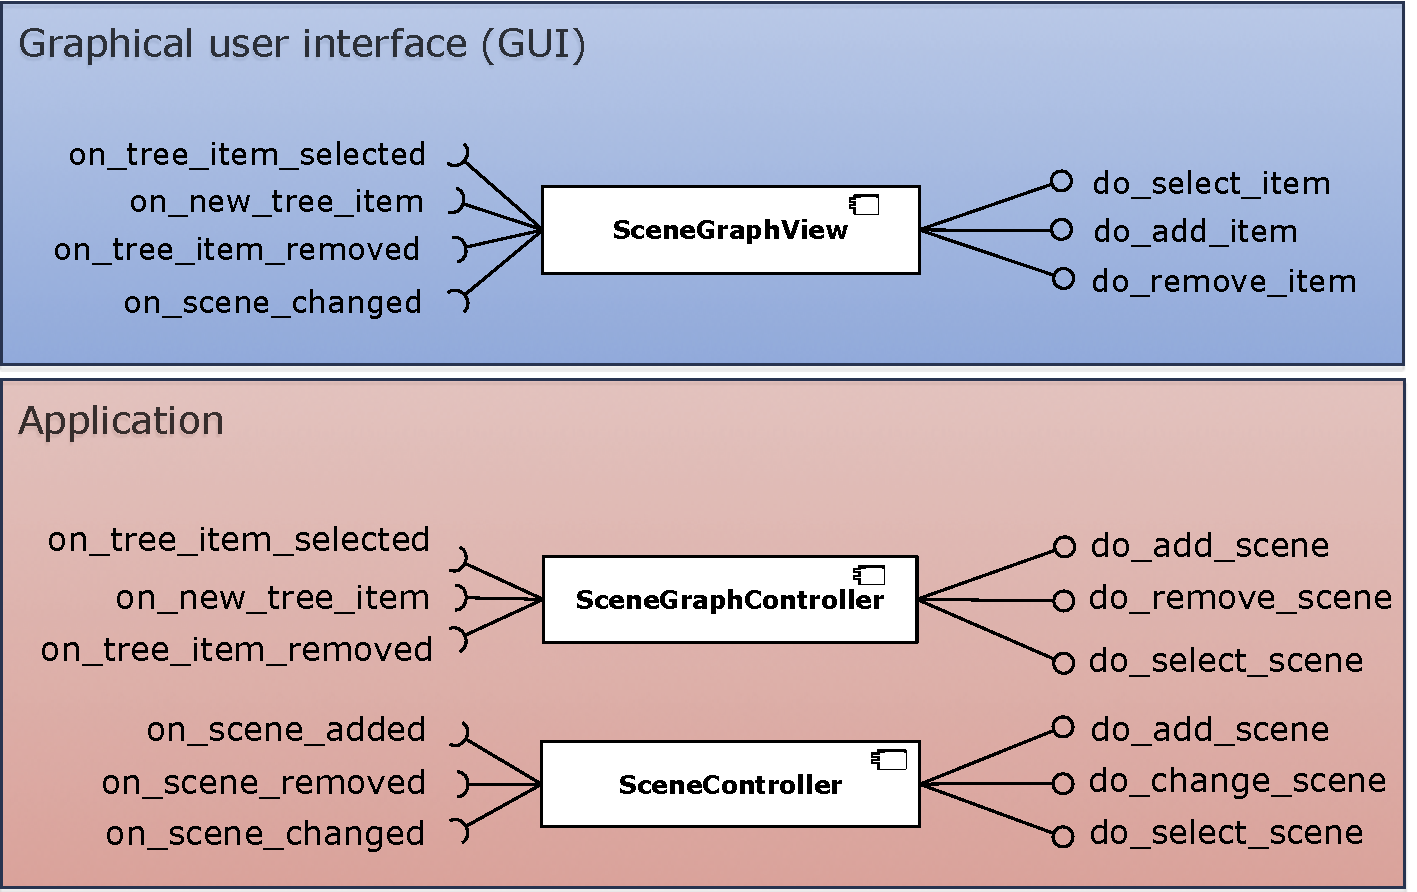
\includegraphics[width=0.95\linewidth]{images/scene-graph-component-diagram}
\end{figure*}

\begin{figure}[ht]
  \caption{Entity relationship diagram of the scene tree component.}
  \label{fig:scene-graph-erd}
  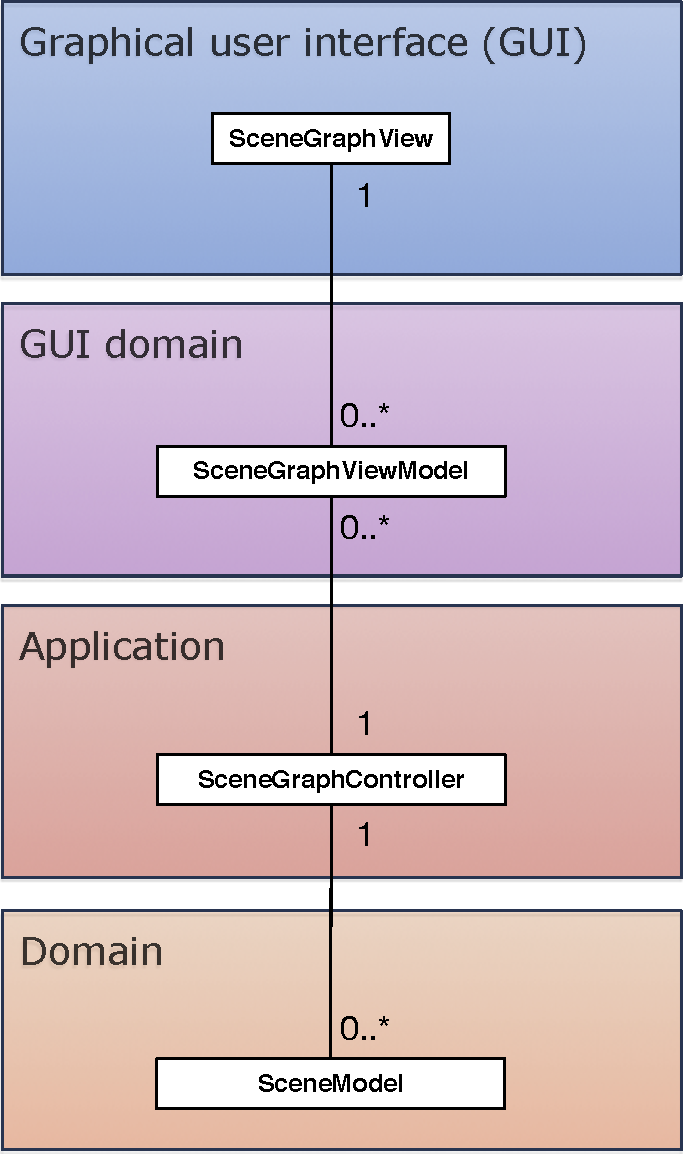
\includegraphics[width=0.75\linewidth]{images/scene-graph-erd}
\end{figure}

\newthought{The scene tree component} enables the scenes of the animation to be
managed. User interaction is provided through a tree-like view, which lets the
user add, remove and select scenes.

% \subsection{Node graph}
% \label{results:subsec:program:node-graph}
% 
% \begin{figure*}[ht]
%   \caption{Component diagram of the node graph component.}
%   \label{fig:node-graph-component-diagram}
%   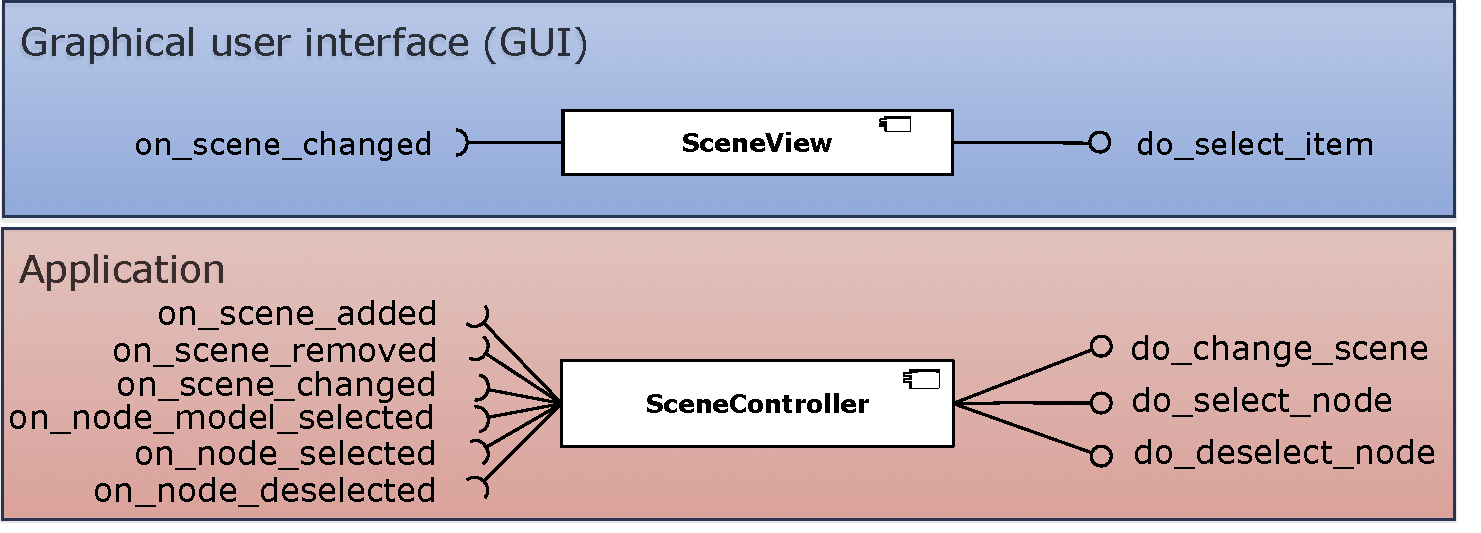
\includegraphics[width=0.95\linewidth]{images/node-graph-component-diagram}
% \end{figure*}
% 
% \begin{figure}[ht]
%   \caption{Entity relationship diagram of the node graph component.}
%   \label{fig:node-graph-erd}
%   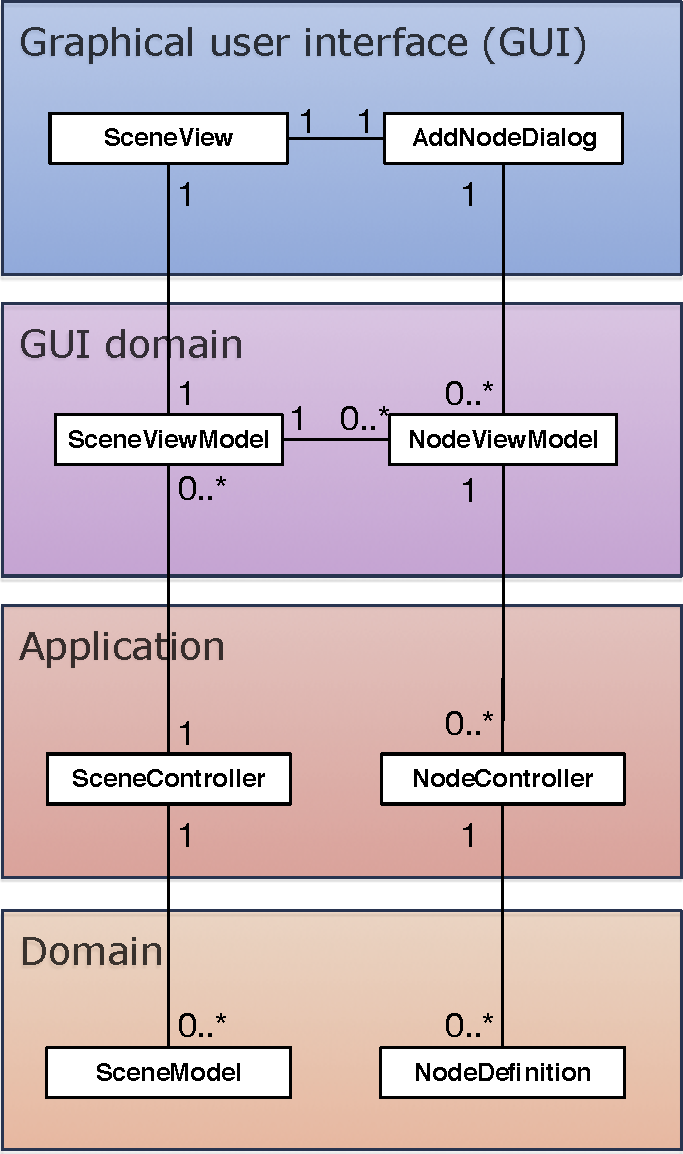
\includegraphics[width=0.75\linewidth]{images/node-graph-erd}
% \end{figure}% -*- mode: latex; coding: utf-8 -*-

\chapter{Discussion and conclusion}
\label{chap:discussion-conclusion}

\todo[inline]{Write chapter.}

% Im Kapitel Diskussion setzt sich die Autorin, der Autor mit den erzielten
% Ergebnissen auseinander. Diese werden interpretiert und mit Erkenntnissen aus
% anderen Studien zur gleichen Fragestellung beurteilt. Die Diskussion schafft die
% nötigen Grundlagen, damit die in der Einleitung formulierte Fragestellung
% möglichst gut und sachlich richtig beantwortet werden kann.

% In den Folgerungen können die wichtigsten Ergebnisse in ihrer kritischen
% Würdigung prägnant zusammengefasst werden. Es wird eine Art Schlussbilanz
% gezogen. Aus der detaillierten Darstellung der Ergebnisse und deren Diskussion
% lässt sich in der Regel eine Antwort auf die Ausgangsfrage ableiten [3, p. 26].
% Die Antwort auf die Fragestellung kann zu Empfeh- lungen für die Ausführung in
% der Praxis oder für weitere Studien führen. Die Folgerungen dürfen keine neuen
% Elemente und Aspekte enthalten, welche nicht schon in den Ergebnissen und in der
% Diskussion behandelt wurden. Wenn die Problemstellung der Arbeit nur sehr wenige
% Folgerungen verlangt, können diese auch als Schlussteil in die Diskussion
% integriert werden.

\newthought{Optional objectives} are the following:
\begin{itemize}
  \item Additional features for the editor, as follows.
  \begin{itemize}
    \item A sequencer, allowing a time-based scheduling of defined scenes.
    \item Additional nodes, such as operations (e.g. replication of objects)
      or post-processing effects (glow/glare, color grading and so on).
  \end{itemize}
  \item Development of a standalone player application. The player allows the
    playback of animations (time-based, compounded scenes in sequential order)
    created with the editor.
\end{itemize}
% Backmatter
%---------------------------------------------------------------------------
\backmatter{}

% Appendix
% -*- mode: latex; coding: utf-8 -*-

\appendix
\part*{Appendix}
\label{part:appendix}

% -*- mode: latex; coding: utf-8 -*-

\chapter{Implementation}
\label{appendix:chap:implementation}

\newthought{To begin with the implementation} of a project, it is necessary to
first think about the goal that one wants to reach and about some basic
structures and guidelines which lead to the fulfillment of that goal.

\newthought{The main goal is} to have a visual animation system, which allows
the creation and rendering of visually appealing scenes, using a graphical user
interface for creation, and a ray tracing based algorithm for
rendering.~\todo{Adapt goal to current state.}

\newthought{The thoughts to reach this goal} were already developed
in~\nameref{chap:fundamentals} and~\nameref{chap:methodologies} and will
therefore not be repeated again.

\newthought{As stated in~\nameref{chap:methodologies}}, the literate programming
paradigm is used to implement the components. To maintain readability only
relevant code fragments are shown in place. The whole code fragments, which are
needed for tangling, are found at~\nameref{chap:code-fragments}.

\newthought{The editor component is described first} as it is the basis for the
whole project and also contains many concepts, that are re-used by the player
component. Before starting with the implementation it is necessary to define
requirements and some kind of framework for the implementation.

% -*- mode: latex; coding: utf-8 -*-

\section{Requirements}
\label{appendix:sec:requirements}

\newthought{The requirements for running the implementation} are currently the
following:

\begin{itemize}
  \item A Unix derivative as operating system (Linux, macOS).
  \item Python~\footnote{\url{http://www.python.org}} version 3.5.x or above
  \item PyQt5~\footnote{%
      \url{https://riverbankcomputing.com/software/pyqt/intro}} version 5.7 or
    above
  \item OpenGL~\footnote{\url{https://www.opengl.org/}} version 3.3 or above
\end{itemize}% -*- mode: latex; coding: utf-8 -*-

\section{Name spaces and project structure}
\label{appendix:sec:name-spaces}

\newthought{To provide a structure for the whole project} and for being able to
stick to the thoughts established in~\nameref{chap:fundamentals}
and~\nameref{chap:methodologies}, it may be wise to structure the project a
certain way.

\newthought{The source code shall be placed} in the~\verb+src+ directory
underneath the main directory. The creation of the single directories is not
explicitly shown, it is done by parts of this documentation which are tangled
but not exported.

\newthought{When dealing with directories and files}, Python uses the
term~\emph{package} for (sub-) directories and~\emph{module} for files within
directories.\footnote{https://docs.python.org/3/reference/import.html\#packages}

\newthought{To prevent having multiple modules having the same name,} name
spaces are
used.\footnote{https://docs.python.org/3/tutorial/classes.html\#python-scopes-and-namespaces}
The main name space shall be analogous to the project's name:~\verb+qde+.
Underneath the source code folder~\verb+src+, each sub-folder represents a
package and acts therefore also as a name space.

\newthought{To allow a whole package and its modules} being
imported~\emph{as modules}, it needs to have at least a file inside,
called~\verb+__init__.py+. Those files may be empty or they may contain
regular source code such as classes or methods.

\section{Coding style}
\label{appendix:sec:coding-style}

\newthought{To stay consistent throughout implementation} of components, a
coding style is applied which is defined as follows.

\begin{itemize}
  \item Classes use camel case, e.g. \verb+class SomeClassName+.
  \item Folders respectively name spaces use only small letters, e.g.
    \verb+foo.bar.baz+.
  \item Methods are all small caps and use underscores as spaces, e.g.
    \verb+some_method_name+.
  \item Signals are methods, which are prefixed by the word~\enquote{do}, e.g.
    \verb+do_something+.
  \item Slots are methods, which are prefixed by the word~\enquote{on}, e.g.
    \verb+on_something+.
  \item Importing is done by the \verb+from Foo import Bar+ syntax, whereas
    \verb+Foo+ is a module and \verb+Bar+ is either a module, a class or a
    method.
\end{itemize}

\subsection{Importing of modules}
\label{appendix:subsec:imports}

\newthought{For the implementation python is used}, as mentioned
in section~\enquote{\nameref{appendix:sec:requirements}}.
Python has~\enquote{batteries included}, which means that it offers a lot of
functionality through various modules, which have to be imported first before
using them. The same applies of course for self written modules. Python offers
multiple possibilities concerning imports, for details
see~\url{https://docs.python.org/3/tutorial/modules.html}. \todo[inline]{Is
direct url reference ok or does this need to be citation?}

However, PEP number 8 recommends to either import modules directly or to import
the needed functionality
directly.~\footnote{\url{https://www.python.org/dev/peps/pep-0020/}}. As defined
by the coding style,~\autoref{subsec:appendix-implementation-coding-style},
imports are done by the \verb+from Foo import Bar+ syntax.

\newthought{The imported modules are always split up:} first the system modules
are imported, modules which are provided by Python itself or by external
libraries, then project-related modules are imported.

\subsection{Framework for implementation}
\label{appendix:subsec:framework}

\newthought{To stay consistent when implementing} classes an methods, it makes
sense to define a rough framework for their implementation, which is as follows:
\begin{enumerate*}
  \item Define necessary signals,
  \item define the constructor and
  \item implement the remaining functionality in terms of methods and slots.
\end{enumerate*}
Concerning the constructor, the following pattern may be applied:
\begin{enumerate*}
  \item Set up the user interface when it is a class concerning the graphical
    user interface,
  \item set up class-specific aspects, such as the name, the tile or an icon,
  \item set up other components used by that class and
  \item initialize the connections, meaning hooking up the defined signals
    with corresponding methods.
\end{enumerate*}

Now, having defined the~\emph{requirements}, a~\emph{project structure},
a~\emph{coding style} and a~\emph{framework for} the
actual~\emph{implementation}, the implementation of the editor may be
approached.
%-*- mode: latex; coding: utf-8 -*-

\chapter{Editor}
\label{appendix:chap:editor}

\newthought{Before diving right into the implementation} of the editor, it may
be good to reconsider what shall actually be implemented, therefore what the
main functionality of the editor is and what its components are.

\newthought{The quintessence of the editor} is to output a structure, be it in
the JSON format or even in bytecode, which defines an animation.

\newthought{An animation} is simply a composition of scenes which run in a
sequential order within a time span. A scene is then a composition of nodes,
which are at the end of their evaluation nothing else as shader specific code
which gets executed on the GPU. As this definition is rather abstract, it may be
easier to define what shall be achieved in terms of content and then work
towards this definition.

\newthought{A very basic definition of what shall be achieved} is the following.
It shall be possible to create an animated scene using the editor application.
The scene shall be composed of two objects, a sphere and a cube. Additionally it
shall have a camera as well as a point light.

The camera shall be placed 5 units in height and 10 units in front of the center
of the scene. The cube shall be placed in the middle of the scene, the sphere
shall have an offset of 5 units to the right and 2 units in depth. The point
light shall be placed 10 units above the center.

Both objects shall have different materials: the cube shall have a dull surface
of any color whereas the sphere shall have a glossy surface of any color.

There shall be an animation of ten seconds duration. During this animation the
sphere shall move towards the cube and they shall merge into a blob-like object.
The camera shall move 5 units towards the two objects during this time.

\newthought{To achieve this overall goal}, while providing an user-friendly
experience, several components are needed. These are the following, being
defined in~\citetitle[pp. 29
ff.]{osterwalder-qde-2016}~\cite{osterwalder-qde-2016}

\begin{description}
  \item[A scene graph] allowing the creation and deletion of scenes. The scene
    graph has at least a root scene.
  \item[A node-based graph] structure allowing the composition of scenes using
    nodes and connections between the nodes. There exists at least a root node
    at the root scene of the scene graph.
  \item[A parameter window] showing parameters of the currently selected graph
    node.
  \item[A rendering window] rendering the currently selected node or scene.
  \item[A sequencer] allowing a time-based scheduling of defined scenes.
\end{description}

However, the above list is not complete. It is somehow intuitively clear, that
there needs to be some~\emph{main component}, which holds all the mentioned
components and allows a proper handling of the application (like managing
resources, shutting down properly and so on).

\newthought{The main component} is composed of a view and a controller, as the
whole architecture uses layers and the MVVMC principle, see
section~\enquote{\nameref{soarch}}. A model is (at least at this point) not
necessary. The view component shall be called~\emph{main window} and its
controller shall be called~\emph{main application}.

\newthought{To preserve clarity} all components are described in discrete
chapters. Although the implementation of the components is very specific, in
terms of the programming language, their logic may be reused later on when
developing the player component.

\newthought{Before implementing} any of these components however, the editor
application needs an entry point, that is a point where the application starts
when being called.

\section{Main entry point}
\label{appendix:sec:editor:main}

\newthought{An entry point} is a point where an application starts when being
called. Python does this by evaluating a special variable within a module,
called~\verb=__name__+. Its value is set to~\verb+'__main__'= if the module
is~\enquote{read from standard input, a script, or from an interactive
prompt.}~\footnote{\url{https://docs.python.org/3/library/__main__.html}}

\newthought{All that the entry point needs to do}, in case of the editor
application, is spawning the editor application, execute it and exit again, as
can be seen below.

\begin{figure}[h]
  \begin{flushleft} \small
\begin{minipage}{\linewidth}\label{scrap11}\raggedright\small
\NWtarget{nuweb?}{} $\langle\,${\itshape Main entry point}\nobreak\ {\footnotesize {?}}$\,\rangle\equiv$
\vspace{-1ex}
\begin{pythoncode}
if __name__ == "__main__":
    app = application.Application(sys.argv)
    status = app.exec()
    sys.exit(status)
  |\NWsep|
\end{pythoncode}
\vspace{1.5ex}
\footnotesize
\begin{list}{}{\setlength{\itemsep}{-\parsep}\setlength{\itemindent}{-\leftmargin}}
\item \NWtxtMacroRefIn\ \NWlink{nuweb?}{?}.

\item{}
\end{list}
\end{minipage}\vspace{4ex}
\end{flushleft}
\caption{Main entry point of the editor application.\newline{}\newline{}Editor
    $\rightarrow$ Main entry point}
  \label{editor:lst:main}
\end{figure}

\newthought{But where to place the main entry point?} A very direct approach
would be to implement that main entry point within the main application
controller. But when running the editor application by calling it from the
command line, calling a controller directly may rather be confusing. Instead it
is more intuitive to have only a minimal entry point which is clearly visible as
such. Therefore the main entry point will be put in a file
called~\verb=editor.py+ which is at the top level of the~\verb+src= directory.

\section{Main application}
\label{appendix:sec:editor:app}

\newthought{The editor application cannot be started yet}, although a main entry
point is defined by now. This is due the fact that there is no such thing as an
editor application yet. Therefore a main application needs to implemented.

\newthought{Qt version 5 is used} through the PyQt5 wrapper, as stated in the
section~\enquote{\nameref{appendix:sec:requirements}}. Therefore all
functionality of Qt 5 may be used. Qt already offers a main application class,
which can be used as a controller. The class is called~\verb=QApplication=.

\newthought{But what does such a main application class actually do?} What is
its functionality? Very roughly sketched, such a type of application initializes
resources, enters a main loop, where it stays until told to shut down, and at
the end it frees the allocated resources again.

Due to the usage of~\verb=QApplication= as super class it is not necessary to
implement a main (event-) loop, as such is provided by Qt
itself~\footnote{http://doc.qt.io/Qt-5/qapplication.html\#exec}.

As the main application initializes resources, it act as central node between the
various layers of the architecture, initializing them and connecting them using
signals.\cite[pp. 37 --- 38]{osterwalder-qde-2016}

\begin{figure}[h]
  \begin{flushleft} \small
\begin{minipage}{\linewidth}\label{scrap12}\raggedright\small
\NWtarget{nuweb?}{} $\langle\,${\itshape Main application declarations}\nobreak\ {\footnotesize {?}}$\,\rangle\equiv$
\vspace{-1ex}
\begin{pythoncode}
|\normalfont{}\fontfamily{}|common.with_logger
class Application(QtWidgets.QApplication):
    """Main application for QDE."""

    |\hbox{$\langle\,${\itshape Main application constructor}\nobreak\ {\footnotesize \NWlink{nuweb?}{?}}$\,\rangle$}|
    |\hbox{$\langle\,${\itshape Main application methods}\nobreak\ {\footnotesize \NWlink{nuweb?}{?}}$\,\rangle$}||\NWsep|
\end{pythoncode}
\vspace{1.5ex}
\footnotesize
\begin{list}{}{\setlength{\itemsep}{-\parsep}\setlength{\itemindent}{-\leftmargin}}
\item \NWtxtMacroRefIn\ \NWlink{nuweb?}{?}.

\item{}
\end{list}
\end{minipage}\vspace{4ex}
\end{flushleft}
\caption{Main application class of the editor
    application.\newline{}\newline{}Editor $\rightarrow$ Application}
  \label{editor:lst:app}
\end{figure}

Therefore it needs to do at least three things:
\begin{enumerate*}
  \item initialize itself,
  \item set up components and
  \item connect components.
  \end{enumerate*}
This all happens when the main application is being initialized through its
constructor.

\begin{figure}[h]
\begin{flushleft} \small
\begin{minipage}{\linewidth}\label{scrap13}\raggedright\small
\NWtarget{nuweb?}{} $\langle\,${\itshape Main application constructor}\nobreak\ {\footnotesize {?}}$\,\rangle\equiv$
\vspace{-1ex}
\begin{pythoncode}
def __init__(self, arguments):
    """Constructor.

    :param arguments: a (variable) list of arguments, that are
                      passed when calling this class.
    :type  argv:      list
    """

    |\hbox{$\langle\,${\itshape Set up internals for main application}\nobreak\ {\footnotesize \NWlink{nuweb?}{?}, \ldots\ }$\,\rangle$}|
    |\hbox{$\langle\,${\itshape Set up components for main application}\nobreak\ {\footnotesize \NWlink{nuweb?}{?}}$\,\rangle$}|
    |\hbox{$\langle\,${\itshape Add root node for main application}\nobreak\ {\footnotesize \NWlink{nuweb?}{?}}$\,\rangle$}|
    |\hbox{$\langle\,${\itshape Set model for scene graph view}\nobreak\ {\footnotesize \NWlink{nuweb?}{?}}$\,\rangle$}|
    |\hbox{$\langle\,${\itshape Load nodes}\nobreak\ {\footnotesize \NWlink{nuweb?}{?}}$\,\rangle$}|
    self.main_window.show()|\NWsep|
\end{pythoncode}
\vspace{1.5ex}
\footnotesize
\begin{list}{}{\setlength{\itemsep}{-\parsep}\setlength{\itemindent}{-\leftmargin}}
\item \NWtxtMacroRefIn\ \NWlink{nuweb?}{?}.

\item{}
\end{list}
\end{minipage}\vspace{4ex}
\end{flushleft}
\caption{Constructor of the editor application
    class.\newline{}\newline{}Editor $\rightarrow$ Application $\rightarrow$
    Constructor} \label{editor:lst:app:constructor}
\end{figure}

\newthought{Setting up the internals} is straight forward: Passing any given
arguments directly to~\verb=QApplication=, setting an application icon, a name
as well as a display name.

\begin{figure}[h]
\begin{flushleft} \small
\begin{minipage}{\linewidth}\label{scrap14}\raggedright\small
\NWtarget{nuweb?}{} $\langle\,${\itshape Set up internals for main application}\nobreak\ {\footnotesize {?}}$\,\rangle\equiv$
\vspace{-1ex}
\begin{pythoncode}
super(Application, self).__init__(arguments)
self.setWindowIcon(QtGui.QIcon("assets/icons/im.png"))
self.setApplicationName("QDE")
self.setApplicationDisplayName("QDE")|\NWsep|
\end{pythoncode}
\vspace{1.5ex}
\footnotesize
\begin{list}{}{\setlength{\itemsep}{-\parsep}\setlength{\itemindent}{-\leftmargin}}
\item \NWtxtMacroDefBy\ \NWlink{nuweb?}{?}\NWlink{nuweb?}{, ?}.
\item \NWtxtMacroRefIn\ \NWlink{nuweb?}{?}.

\item{}
\end{list}
\end{minipage}\vspace{4ex}
\end{flushleft}
\caption{Setting up the internals for the main application class.
  \newline{}\newline{}Editor $\rightarrow$ Application $\rightarrow$
  Constructor} \label{editor:lst:app:constructor:internals}
\end{figure}

The other two steps, setting up the components and connecting them can however
not be done at this point, as there simply are no components available. A
component to start with is the view component of the main application, the main
window.

\section{Main window}
\label{appendix:sec:editor:main-window}

\newthought{Having a very basic implementation} of the main application, its
view component, the main window, can now be implemented and then be set up by
the main application.

\newthought{The main functionality} of the main window is to set up the actual
user interface, containing all the views of the components. Qt offers the class
\verb=QMainWindow= from which~\verb=MainWindow= may inherit.

\begin{figure}
\begin{flushleft} \small
\begin{minipage}{\linewidth}\label{scrap15}\raggedright\small
\NWtarget{nuweb?}{} $\langle\,${\itshape Main window declarations}\nobreak\ {\footnotesize {?}}$\,\rangle\equiv$
\vspace{-1ex}
\begin{pythoncode}
|\normalfont{}\fontfamily{}|common.with_logger
class MainWindow(QtWidgets.QMainWindow):
    """The main window class.
    Acts as main view for the QDE editor application.
    """

    |\hbox{$\langle\,${\itshape Main window signals}\nobreak\ {\footnotesize \NWlink{nuweb?}{?}}$\,\rangle$}|

    |\hbox{$\langle\,${\itshape Main window methods}\nobreak\ {\footnotesize \NWlink{nuweb?}{?}, \ldots\ }$\,\rangle$}|
|\NWsep|
\end{pythoncode}
\vspace{1.5ex}
\footnotesize
\begin{list}{}{\setlength{\itemsep}{-\parsep}\setlength{\itemindent}{-\leftmargin}}
\item \NWtxtMacroRefIn\ \NWlink{nuweb?}{?}.

\item{}
\end{list}
\end{minipage}\vspace{4ex}
\end{flushleft}
\caption{Main window class of the editor application.
  \newline{}\newline{}Editor $\rightarrow$ Main window}
  \label{editor:lst:main-window}
\end{figure}
% AT<Main window slotsAT>

\newthought{For being able to shut down} the main application and therefore the
main window, they need to react to a request for shutting down, either by a
keyboard shortcut or a menu command. However, the main window is not able to
force the main application to quit by itself. It would be possible to pass the
main window a reference to the application, but that would lead to tight
coupling and is therefore not considered as an option. Signals and slots allow
exactly such cross-layer communication without coupling components tightly.

\newthought{To avoid tight coupling} a signal within the main window is
introduced, which tells the main application to shut down. A fitting name for
the signal might be~\verb=do_close=.

\begin{figure}
\begin{flushleft} \small
\begin{minipage}{\linewidth}\label{scrap16}\raggedright\small
\NWtarget{nuweb?}{} $\langle\,${\itshape Main window signals}\nobreak\ {\footnotesize {?}}$\,\rangle\equiv$
\vspace{-1ex}
\begin{pythoncode}
do_close = QtCore.pyqtSignal()|\NWsep|
\end{pythoncode}
\vspace{1.5ex}
\footnotesize
\begin{list}{}{\setlength{\itemsep}{-\parsep}\setlength{\itemindent}{-\leftmargin}}
\item \NWtxtMacroRefIn\ \NWlink{nuweb?}{?}.

\item{}
\end{list}
\end{minipage}\vspace{4ex}
\end{flushleft}
\caption{Definition of the~\texttt{do\_close} signal of the main window class.
  \newline{}\newline{}Editor $\rightarrow$ Main window $\rightarrow$ Signals}
\label{editor:lst:main-window:signals}
\end{figure}

Now, that the signal for closing the window and the application is defined, two
additional things need to be considered: The emission of the signal by
the main window itself as well as the consumption of the signal by a slot of
other classes.

The signal shall be emitted when the escape key on the keyboard is pressed or
when the corresponding menu item was selected. As there is no menu at the
moment, only the key pressed event is implemented by now.

\begin{figure}
\begin{flushleft} \small
\begin{minipage}{\linewidth}\label{scrap17}\raggedright\small
\NWtarget{nuweb?}{} $\langle\,${\itshape Main window methods}\nobreak\ {\footnotesize {?}}$\,\rangle\equiv$
\vspace{-1ex}
\begin{pythoncode}
def __init__(self, parent=None):
    """Constructor."""

    super(MainWindow, self).__init__(parent)
    self.setup_ui()

def keyPressEvent(self, event):
    """Gets triggered when a key press event is raised.

    :param event: holds the triggered event.
    :type  event: QKeyEvent
    """

    if event.key() == QtCore.Qt.Key_Escape:
        self.do_close.emit()
    else:
        super(MainWindow, self).keyPressEvent(event)
|\NWsep|
\end{pythoncode}
\vspace{1.5ex}
\footnotesize
\begin{list}{}{\setlength{\itemsep}{-\parsep}\setlength{\itemindent}{-\leftmargin}}
\item \NWtxtMacroDefBy\ \NWlink{nuweb?}{?}\NWlink{nuweb?}{, ?}.
\item \NWtxtMacroRefIn\ \NWlink{nuweb?}{?}.

\item{}
\end{list}
\end{minipage}\vspace{4ex}
\end{flushleft}
\caption{Definition of methods for the main window class.
  \newline{}\newline{}Editor $\rightarrow$ Main window $\rightarrow$ Methods}
\label{editor:lst:main-window:methods}
\end{figure}

% For emitting the signal when selecting a menu entry, an action needs to be
% defined which is then attached to the menu entry. The action emits a signal as
% soon as the menu entry was clicked. It is however not possible to trigger the
% defined~\verb=do_close= signal using the actions signal. There a slot needs to
% be defined which then in its turn triggers~\verb=do_close=.

\newthought{The main window can now be set up} by the main application
controller, which also listens to the~\verb=do_close= signal through the
inherited~\verb=quit= slot.

\begin{figure}
\begin{flushleft} \small
\begin{minipage}{\linewidth}\label{scrap18}\raggedright\small
\NWtarget{nuweb?}{} $\langle\,${\itshape Set up components for main application}\nobreak\ {\footnotesize {?}}$\,\rangle\equiv$
\vspace{-1ex}
\begin{pythoncode}
|\hbox{$\langle\,${\itshape Set up controllers for main application}\nobreak\ {\footnotesize \NWlink{nuweb?}{?}, \ldots\ }$\,\rangle$}|
|\hbox{$\langle\,${\itshape Connect controllers for main application}\nobreak\ {\footnotesize \NWlink{nuweb?}{?}, \ldots\ }$\,\rangle$}|
|\hbox{$\langle\,${\itshape Set up main window for main application}\nobreak\ {\footnotesize \NWlink{nuweb?}{?}}$\,\rangle$}||\NWsep|
\end{pythoncode}
\vspace{1.5ex}
\footnotesize
\begin{list}{}{\setlength{\itemsep}{-\parsep}\setlength{\itemindent}{-\leftmargin}}
\item \NWtxtMacroRefIn\ \NWlink{nuweb?}{?}.

\item{}
\end{list}
\end{minipage}\vspace{4ex}
\end{flushleft}
\caption{Setting up of components for the main application class.
  \newline{}\newline{}Editor $\rightarrow$ Main application $\rightarrow$
  Constructor}
\label{editor:lst:main-application:constructor:methods}
\end{figure}

\begin{figure}
\begin{flushleft} \small
\begin{minipage}{\linewidth}\label{scrap19}\raggedright\small
\NWtarget{nuweb?}{} $\langle\,${\itshape Set up main window for main application}\nobreak\ {\footnotesize {?}}$\,\rangle\equiv$
\vspace{-1ex}
\begin{pythoncode}
self.main_window = qde_main_window.MainWindow()
self.main_window.do_close.connect(self.quit)
|\hbox{$\langle\,${\itshape Connect main window components}\nobreak\ {\footnotesize \NWlink{nuweb?}{?}, \ldots\ }$\,\rangle$}||\NWsep|
\end{pythoncode}
\vspace{1.5ex}
\footnotesize
\begin{list}{}{\setlength{\itemsep}{-\parsep}\setlength{\itemindent}{-\leftmargin}}
\item \NWtxtMacroRefIn\ \NWlink{nuweb?}{?}.

\item{}
\end{list}
\end{minipage}\vspace{4ex}
\end{flushleft}
\caption{Set up of the editor main window and its signals from within the main
  application. \newline{}\newline{}Editor $\rightarrow$ Main application
  $\rightarrow$ Constructor}
\label{editor:lst:main-application:constructor:main-window}
\end{figure}

The used view component for the main window,~\verb=QMainWindow=, needs at least
a central widget with a layout for being
rendered.~\footnote{http://doc.qt.io/qt-5/qmainwindow.html\#creating-main-window-components}

\newthought{As the main window will set up and hold} the whole layout for the
application through multiple view components, a method~\verb=setup_ui= is
introduced, which sets up the whole layout. The method creates a central widget
containing a grid layout.

\newthought{Targeting a look} as proposed in~\citetitle[p.
9]{osterwalder-qde-2016}, a simple grid layout does however not provide enough
possibilities. Instead a horizontal box layout in combination with splitters is
used.

Recalling the components, the following layout is approached:

\begin{itemize}
\item{%
    A scene graph, on the left of the window, covering the whole height.}
\item{%
    A node graph on the right of the scene graph, covering as much height as
    possible.}
\item{%
    A view for showing the properties (and therefore parameters) of the selected
    node on the right of the node graph, covering as much height as possible.}
\item{%
    A display for rendering the selected node, on the right of the properties
    view, covering as much height as possible}
\item{%
    A sequencer at the right of the scene graph and below the other components
    at the bottom of the window, covering as much width as possible}
\end{itemize}

\todo[inline]{Provide a picture of the layout here.}

\begin{figure*}
\begin{flushleft} \small
\begin{minipage}{\linewidth}\label{scrap20}\raggedright\small
\NWtarget{nuweb?}{} $\langle\,${\itshape Main window methods}\nobreak\ {\footnotesize {?}}$\,\rangle+\equiv$
\vspace{-1ex}
\begin{pythoncode}
def setup_ui(self):
    """Sets up the user interface specific components."""

    self.setObjectName('MainWindow')
    self.setWindowTitle('QDE')
    self.resize(1024, 768)
    self.move(100, 100)
    # Ensure that the window is not hidden behind other windows
    self.activateWindow()

    central_widget = QtWidgets.QWidget(self)
    central_widget.setObjectName('central_widget')
    grid_layout = QtWidgets.QGridLayout(central_widget)
    central_widget.setLayout(grid_layout)
    self.setCentralWidget(central_widget)
    self.statusBar().showMessage('Ready.')

    horizontal_layout_widget = QtWidgets.QWidget(central_widget)
    horizontal_layout_widget.setObjectName('horizontal_layout_widget')
    horizontal_layout_widget.setGeometry(QtCore.QRect(12, 12, 781, 541))
    horizontal_layout_widget.setSizePolicy(QtWidgets.QSizePolicy.MinimumExpanding,
    QtWidgets.QSizePolicy.MinimumExpanding)
    grid_layout.addWidget(horizontal_layout_widget, 0, 0)

    horizontal_layout = QtWidgets.QHBoxLayout(horizontal_layout_widget)
    horizontal_layout.setObjectName('horizontal_layout')
    horizontal_layout.setContentsMargins(0, 0, 0, 0)

    self.scene_graph_view = guiscene.SceneGraphView()
    self.scene_graph_view.setObjectName('scene_graph_view')
    self.scene_graph_view.setMaximumWidth(300)
    horizontal_layout.addWidget(self.scene_graph_view)

    |\hbox{$\langle\,${\itshape Set up scene view in main window}\nobreak\ {\footnotesize \NWlink{nuweb?}{?}}$\,\rangle$}|
    |\hbox{$\langle\,${\itshape Set up parameter view in main window}\nobreak\ {\footnotesize ?}$\,\rangle$}|
    |\hbox{$\langle\,${\itshape Set up render view in main window}\nobreak\ {\footnotesize ?}$\,\rangle$}|

    horizontal_splitter = QtWidgets.QSplitter()
    |\hbox{$\langle\,${\itshape Add render view to horizontal splitter in main window}\nobreak\ {\footnotesize ?}$\,\rangle$}|
    |\hbox{$\langle\,${\itshape Add parameter view to horizontal splitter in main window}\nobreak\ {\footnotesize ?}$\,\rangle$}|

    vertical_splitter = QtWidgets.QSplitter()
    vertical_splitter.setOrientation(QtCore.Qt.Vertical)
    vertical_splitter.addWidget(horizontal_splitter)
    |\hbox{$\langle\,${\itshape Add scene view to vertical splitter in main window}\nobreak\ {\footnotesize \NWlink{nuweb?}{?}}$\,\rangle$}|

    horizontal_layout.addWidget(vertical_splitter)
|\NWsep|
\end{pythoncode}
\vspace{1.5ex}
\footnotesize
\begin{list}{}{\setlength{\itemsep}{-\parsep}\setlength{\itemindent}{-\leftmargin}}
\item \NWtxtMacroDefBy\ \NWlink{nuweb?}{?}\NWlink{nuweb?}{, ?}.
\item \NWtxtMacroRefIn\ \NWlink{nuweb?}{?}.

\item{}
\end{list}
\end{minipage}\vspace{4ex}
\end{flushleft}
\caption{Set up of the user interface of the editor's  main window.
  \newline{}\newline{}Editor $\rightarrow$ Main window
  $\rightarrow$ Methods}
\label{editor:lst:main-window:methods:setup-ui}
\end{figure*}

All the above taken actions to lay out the main window change nothing in the
window's yet plain appearance. This is quite obvious, as none of the actual
components are implemented yet.

\newthought{A good starting point} for the implementation of the remaining
components might be the scene graph, as it might be the most straight-forward
component to implement.

% -*- mode: latex; coding: utf-8 -*-

\chapter{Scene graph}
\label{appendix:chap:scene-graph}

\newthought{The scene graph component} has two aspects to consider, as mentioned
in chapter~\enquote{\nameref{appendix:chap:editor}}:
\begin{enumerate*}
  \item a graphical aspect as well as
  \item its data structure.
\end{enumerate*}

\todo[inline]{Define what a scene is by prose and code.}

As described in subsection~\enquote{\nameref{results:subsec:software-design}},
two kinds of models are used. A domain model, containing the actual data and a
view model, which holds a reference to its corresponding domain model.

% \todo[inline]{Check whether to move into procedure.}
% Both models are managed by the same controller. View models are displayed by views,
% e.g. node view models in the node graph view.
%
% Therefore the controller of the scene graph will manage instances of scene
% domain models whereas the view of the scene graph will display a tree of scene
% view models.

As the domain model builds the basis for the whole (data-) structure, it is
implemented first.

\begin{figure}
\begin{flushleft} \small
\begin{minipage}{\linewidth}\label{scrap21}\raggedright\small
\NWtarget{nuweb?}{} $\langle\,${\itshape Scene model declarations}\nobreak\ {\footnotesize {?}}$\,\rangle\equiv$
\vspace{-1ex}
\begin{pythoncode}
class SceneModel(object):
    """The scene model.
    It is used as a base class for scene instances within the
    whole system.
    """

    |\hbox{$\langle\,${\itshape Scene model signals}\nobreak\ {\footnotesize ?}$\,\rangle$}|
    |\hbox{$\langle\,${\itshape Scene model methods}\nobreak\ {\footnotesize \NWlink{nuweb?}{?}}$\,\rangle$}|
    |\hbox{$\langle\,${\itshape Scene model slots}\nobreak\ {\footnotesize ?}$\,\rangle$}||\NWsep|
\end{pythoncode}
\vspace{1.5ex}
\footnotesize
\begin{list}{}{\setlength{\itemsep}{-\parsep}\setlength{\itemindent}{-\leftmargin}}
\item \NWtxtMacroRefIn\ \NWlink{nuweb?}{?}.

\item{}
\end{list}
\end{minipage}\vspace{4ex}
\end{flushleft}
\caption{Definition of the scene model class, which acts as a base class for
scene instances within the whole application.
  \newline{}\newline{}Editor $\rightarrow$ Scene model}
\label{editor:lst:scene-model}
\end{figure}

\newthought{The only known fact} at this point is, that a scene is a composition
of nodes and therefore holds its nodes as a list. Additionally it holds a
reference to its parent.

\begin{figure}
\begin{flushleft} \small
\begin{minipage}{\linewidth}\label{scrap22}\raggedright\small
\NWtarget{nuweb?}{} $\langle\,${\itshape Scene model methods}\nobreak\ {\footnotesize {?}}$\,\rangle\equiv$
\vspace{-1ex}
\begin{pythoncode}
def __init__(self, parent=None):
    """Constructor.

    :param parent: the parent scene of this scene. The parent is
                   None if the current scene is the root scene.
    :type parent:  SceneModel
    """

    self.id_ = uuid.uuid4()
    self.nodes = []
    self.parent = parent|\NWsep|
\end{pythoncode}
\vspace{1.5ex}
\footnotesize
\begin{list}{}{\setlength{\itemsep}{-\parsep}\setlength{\itemindent}{-\leftmargin}}
\item \NWtxtMacroRefIn\ \NWlink{nuweb?}{?}.

\item{}
\end{list}
\end{minipage}\vspace{4ex}
\end{flushleft}
\caption{The constructor of the scene model.
  \newline{}\newline{}Editor $\rightarrow$ Scene model $\rightarrow$ Constructor}
\label{editor:lst:scene-model:constructor}
\end{figure}

\newthought{The counter part of the domain model} is the view model. View models
are used to visually represent something within the graphical user interface and
they provide an interface to the~\verb=domain= layer. To this point, a simple
reference in terms of an attribute is used as interface, which may be changed
later on.

Concerning the user interface, a view model must fulfill the requirements posed
by the user interface's corresponding component. In this case this are actually
two components: the scene graph view as well as the scene view.

It would therefore make sense the use one view model for both components, but
this is not possible as the view model of the scene view,~\verb=QGraphicsScene=,
uses its own data model.

Therefore~\verb=QObject= will be used for the scene graph view model
and~\verb=QGraphicsScene= will be used for the scene view model.

\begin{figure}
\begin{flushleft} \small
\begin{minipage}{\linewidth}\label{scrap23}\raggedright\small
\NWtarget{nuweb?}{} $\langle\,${\itshape Scene graph view model declarations}\nobreak\ {\footnotesize {?}}$\,\rangle\equiv$
\vspace{-1ex}
\begin{pythoncode}
class SceneGraphViewModel(Qt.QObject):
    """View model representing scene graph items.

    The SceneGraphViewModel corresponds to an entry within the
    scene graph. It is used by the QAbstractItemModel class and
    must therefore at least provide a name and a row.
    """

    |\hbox{$\langle\,${\itshape Scene graph view model signals}\nobreak\ {\footnotesize ?}$\,\rangle$}|
    |\hbox{$\langle\,${\itshape Scene graph view model constructor}\nobreak\ {\footnotesize \NWlink{nuweb?}{?}, \ldots\ }$\,\rangle$}|
    |\hbox{$\langle\,${\itshape Scene graph view model methods}\nobreak\ {\footnotesize \NWlink{nuweb?}{?}, \ldots\ }$\,\rangle$}|
    |\hbox{$\langle\,${\itshape Scene graph view model slots}\nobreak\ {\footnotesize ?}$\,\rangle$}|
|\NWsep|
\end{pythoncode}
\vspace{1.5ex}
\footnotesize
\begin{list}{}{\setlength{\itemsep}{-\parsep}\setlength{\itemindent}{-\leftmargin}}
\item \NWtxtMacroRefIn\ \NWlink{nuweb?}{?}.

\item{}
\end{list}
\end{minipage}\vspace{4ex}
\end{flushleft}
\caption{Definition of the scene graph view model class, which corresponds to an
  entry within the scene graph.
  \newline{}\newline{}Editor $\rightarrow$ Scene graph view model}
\label{editor:lst:scene-graph-view-model}
\end{figure}

In terms of the scene graph, the view model must provide at least a name and a
row. In addition, as written above, it holds a reference to the domain model.

\begin{figure}
\begin{flushleft} \small
\begin{minipage}{\linewidth}\label{scrap24}\raggedright\small
\NWtarget{nuweb?}{} $\langle\,${\itshape Scene graph view model constructor}\nobreak\ {\footnotesize {?}}$\,\rangle\equiv$
\vspace{-1ex}
\begin{pythoncode}
def __init__(
        self,
        row,
        domain_object,
        name=QtCore.QCoreApplication.translate(
            'SceneGraphViewModel', 'New scene'
        ),
        parent=None
):
    """Constructor.

    :param row:           The row the view model is in.
    :type  row:           int
    :param domain_object: Reference to a scene model.
    :type  domain_object: qde.editor.domain.scene.SceneModel
    :param name:          The name of the view model, which will
                          be displayed in the scene graph.
    :type  name:          str
    :param parent:        The parent of the current view model
                          within the scene graph.
    :type parent:         qde.editor.gui_domain.scene.
                          SceneGraphViewModel
    """

    super(SceneGraphViewModel, self).__init__(parent)

    self.id_ = domain_object.id_
    self.row  = row
    self.domain_object = domain_object
    self.name = name
|\NWsep|
\end{pythoncode}
\vspace{1.5ex}
\footnotesize
\begin{list}{}{\setlength{\itemsep}{-\parsep}\setlength{\itemindent}{-\leftmargin}}
\item \NWtxtMacroDefBy\ \NWlink{nuweb?}{?}\NWlink{nuweb?}{, ?}.
\item \NWtxtMacroRefIn\ \NWlink{nuweb?}{?}.

\item{}
\end{list}
\end{minipage}\vspace{4ex}
\end{flushleft}
\caption{The constructor of the scene graph view model.
  \newline{}\newline{}Editor $\rightarrow$ Scene graph view model $\rightarrow$
  Constructor}
\label{editor:lst:scene-graph-view-model:constructor}
\end{figure}

\newthought{Scenes may now be instantiated,} it is although necessary to manage
scenes in a controlled manner. Therefore the class~\verb=SceneGraphController=
will now be implemented, for being able to manage scenes.

As the scene graph shall be built as a tree structure, an appropriate data
structure is needed. Qt provides the~\verb=QTreeWidget= class, but that
class is in this case not suitable, as it does not separate the data from its
representation, as stated by Qt:~\enquote{Developers who do not need the flexibility of
the Model/View framework can use this class to create simple hierarchical lists
very easily. A more flexible approach involves combining a QTreeView with a
standard item model. This allows the storage of data to be separated from its
representation.}\footnote{http://doc.qt.io/qt-5/qtreewidget.html\#details}

\newthought{Such a standard item model}
is~\verb=QAbstractItemModel=\footnote{\label{footnote:qabstractitemmodel}
http://doc.qt.io/qt-5/qabstractitemmodel.html}, which is used as a base class
for the scene graph controller.

\begin{figure}
\begin{flushleft} \small
\begin{minipage}{\linewidth}\label{scrap25}\raggedright\small
\NWtarget{nuweb?}{} $\langle\,${\itshape Scene graph controller declarations}\nobreak\ {\footnotesize {?}}$\,\rangle\equiv$
\vspace{-1ex}
\begin{pythoncode}
|\normalfont{}\fontfamily{}|common.with_logger
class SceneGraphController(QtCore.QAbstractItemModel):
    """The scene graph controller.
    A controller for managing the scene graph by adding,
    editing and removing scenes.
    """

    |\hbox{$\langle\,${\itshape Scene graph controller signals}\nobreak\ {\footnotesize \NWlink{nuweb?}{?}}$\,\rangle$}|
    |\hbox{$\langle\,${\itshape Scene graph controller constructor}\nobreak\ {\footnotesize \NWlink{nuweb?}{?}, \ldots\ }$\,\rangle$}|
    |\hbox{$\langle\,${\itshape Scene graph controller methods}\nobreak\ {\footnotesize \NWlink{nuweb?}{?}, \ldots\ }$\,\rangle$}|
    |\hbox{$\langle\,${\itshape Scene graph controller slots}\nobreak\ {\footnotesize \NWlink{nuweb?}{?}}$\,\rangle$}|
|\NWsep|
\end{pythoncode}
\vspace{1.5ex}
\footnotesize
\begin{list}{}{\setlength{\itemsep}{-\parsep}\setlength{\itemindent}{-\leftmargin}}
\item \NWtxtMacroRefIn\ \NWlink{nuweb?}{?}.

\item{}
\end{list}
\end{minipage}\vspace{4ex}
\end{flushleft}
\caption{The scene graph controller, inherting from~\texttt{QAbstractItemModel}.
  \newline{}\newline{}Editor $\rightarrow$ Scene graph controller}
\label{editor:lst:scene-graph-controller}
\end{figure}

\newthought{As at this point the functionality} of the scene graph controller is
not fully known, the constructor simply initializes its parent class and an
empty list of scenes.

\begin{figure}
\begin{flushleft} \small
\begin{minipage}{\linewidth}\label{scrap26}\raggedright\small
\NWtarget{nuweb?}{} $\langle\,${\itshape Scene graph controller constructor}\nobreak\ {\footnotesize {?}}$\,\rangle\equiv$
\vspace{-1ex}
\begin{pythoncode}
def __init__(self, parent=None):
    """Constructor.

    :param parent: The parent of the current view model within
                    the scene graph.
    :type parent:  qde.editor.application.SceneGraphController
    """

    super(SceneGraphController, self).__init__(parent)
|\NWsep|
\end{pythoncode}
\vspace{1.5ex}
\footnotesize
\begin{list}{}{\setlength{\itemsep}{-\parsep}\setlength{\itemindent}{-\leftmargin}}
\item \NWtxtMacroDefBy\ \NWlink{nuweb?}{?}\NWlink{nuweb?}{, ?}.
\item \NWtxtMacroRefIn\ \NWlink{nuweb?}{?}.

\item{}
\end{list}
\end{minipage}\vspace{4ex}
\end{flushleft}
\caption{Constructor of the scene graph controller.
  \newline{}\newline{}Editor $\rightarrow$ Scene graph controller $\rightarrow$
  Constructor}
\label{editor:lst:scene-graph-controller:constructor}
\end{figure}

\newthought{The scene graph controller holds and manages scene data.} Therefore
it needs to have at least a root node. As the controller manages both, domain
models and the view models, it needs to create both models.

Due to the dependencies of other components this cannot be done within the
constructor, as components depending on the scene graph controller may not be
listening to its signals at this point. Therefore this is done in a separate
method called~\verb=add_root_node=.

\begin{figure}
\begin{flushleft} \small
\begin{minipage}{\linewidth}\label{scrap27}\raggedright\small
\NWtarget{nuweb?}{} $\langle\,${\itshape Scene graph controller add root node}\nobreak\ {\footnotesize {?}}$\,\rangle\equiv$
\vspace{-1ex}
\begin{pythoncode}
def add_root_node(self):
    """Add a root node to the data structure.
    """

    if self.root_node is None:
        root_node = domain_scene.SceneModel()
        self.view_root_node = guidomain_scene.SceneGraphViewModel(
            row=0,
            domain_object=root_node,
            name=QtCore.QCoreApplication.translate(
                __class__.__name__, 'Root scene'
            )
        )
        self.do_add_scene.emit(root_node)
        self.layoutChanged.emit()
        self.logger.debug("Added root node")
    else:
        self.logger.warn((
            "Not (re-) adding root node, already"
            "present!"
        ))
|\NWsep|
\end{pythoncode}
\vspace{1.5ex}
\footnotesize
\begin{list}{}{\setlength{\itemsep}{-\parsep}\setlength{\itemindent}{-\leftmargin}}
\item \NWtxtMacroRefIn\ \NWlink{nuweb?}{?}.

\item{}
\end{list}
\end{minipage}\vspace{4ex}
\end{flushleft}
\begin{flushleft} \small
\begin{minipage}{\linewidth}\label{scrap28}\raggedright\small
\NWtarget{nuweb?}{} $\langle\,${\itshape Scene graph controller methods}\nobreak\ {\footnotesize {?}}$\,\rangle\equiv$
\vspace{-1ex}
\begin{pythoncode}
|\hbox{$\langle\,${\itshape Scene graph controller add root node}\nobreak\ {\footnotesize \NWlink{nuweb?}{?}}$\,\rangle$}|
|\NWsep|
\end{pythoncode}
\vspace{1.5ex}
\footnotesize
\begin{list}{}{\setlength{\itemsep}{-\parsep}\setlength{\itemindent}{-\leftmargin}}
\item \NWtxtMacroDefBy\ \NWlink{nuweb?}{?}\NWlink{nuweb?}{, ?}\NWlink{nuweb?}{, ?}\NWlink{nuweb?}{, ?}\NWlink{nuweb?}{, ?}\NWlink{nuweb?}{, ?}\NWlink{nuweb?}{, ?}\NWlink{nuweb?}{, ?}\NWlink{nuweb?}{, ?}.
\item \NWtxtMacroRefIn\ \NWlink{nuweb?}{?}.

\item{}
\end{list}
\end{minipage}\vspace{4ex}
\end{flushleft}
\caption{A method to add the root node from within the scene graph controller.
  \newline{}\newline{}Editor $\rightarrow$ Scene graph controller $\rightarrow$
  Methods}
\label{editor:lst:scene-graph-controller:methods:add-root-node}
\end{figure}

The root scene can now be added by the main application, as all necessary
components are set up.

\begin{figure}
\begin{flushleft} \small
\begin{minipage}{\linewidth}\label{scrap29}\raggedright\small
\NWtarget{nuweb?}{} $\langle\,${\itshape Add root node for main application}\nobreak\ {\footnotesize {?}}$\,\rangle\equiv$
\vspace{-1ex}
\begin{pythoncode}
self.scene_graph_controller.add_root_node()
|\NWsep|
\end{pythoncode}
\vspace{1.5ex}
\footnotesize
\begin{list}{}{\setlength{\itemsep}{-\parsep}\setlength{\itemindent}{-\leftmargin}}
\item \NWtxtMacroRefIn\ \NWlink{nuweb?}{?}.

\item{}
\end{list}
\end{minipage}\vspace{4ex}
\end{flushleft}
\caption{The root node of the scene graph being added by the main application.
  \newline{}\newline{}Editor $\rightarrow$ Main application $\rightarrow$
  Constructor}
\label{editor:lst:main-application:constructor:add-root-node}
\end{figure}

\newthought{The scene graph controller must also provide the header data,} which
is used to display the header within the view (due to the usage of the Qt view
model~\todo{Add reference to Qt's view model}). As header data the name of the
scenes as well as the number of nodes a scene contains shall be displayed.

\begin{figure}
\begin{flushleft} \small
\begin{minipage}{\linewidth}\label{scrap30}\raggedright\small
\NWtarget{nuweb?}{} $\langle\,${\itshape Scene graph controller constructor}\nobreak\ {\footnotesize {?}}$\,\rangle+\equiv$
\vspace{-1ex}
\begin{pythoncode}
    self.header_data = [
        QtCore.QCoreApplication.translate(
            __class__.__name__, 'Name'
        ),
        QtCore.QCoreApplication.translate(
            __class__.__name__, '# Nodes'
        )
    ]
    self.root_node = None
    self.view_root_node = None|\NWsep|
\end{pythoncode}
\vspace{1.5ex}
\footnotesize
\begin{list}{}{\setlength{\itemsep}{-\parsep}\setlength{\itemindent}{-\leftmargin}}
\item \NWtxtMacroDefBy\ \NWlink{nuweb?}{?}\NWlink{nuweb?}{, ?}.
\item \NWtxtMacroRefIn\ \NWlink{nuweb?}{?}.

\item{}
\end{list}
\end{minipage}\vspace{4ex}
\end{flushleft}
\caption{Initialization of the header data and the root node of the scene graph.
  \newline{}\newline{}Editor $\rightarrow$ Scene graph controller $\rightarrow$
  Constructor}
\label{editor:lst:scene-graph-controller:constructor:header-data}
\end{figure}

% TODO: Check if needed
% Before implementing the actual methods, it is important to think about the
% attributes, that the scene graph controller will have, as attributes define and
% influence the methods.

\newthought{As QAbstractItemModel is used as a basis} for the scene graph
controller, some methods must be implemented at very least:~\enquote{When
subclassing QAbstractItemModel, at the very least you must implement index(),
parent(), rowCount(), columnCount(), and data(). These functions are used in all
read-only models, and form the basis of editable
models.}\footref{footnote:qabstractitemmodel}

\newthought{The method index} returns the position of an item in the (data-)
model for a given row and column below a parent item.

\begin{figure}
\begin{flushleft} \small
\begin{minipage}{\linewidth}\label{scrap31}\raggedright\small
\NWtarget{nuweb?}{} $\langle\,${\itshape Scene graph controller methods}\nobreak\ {\footnotesize {?}}$\,\rangle+\equiv$
\vspace{-1ex}
\begin{pythoncode}
def index(self, row, column, parent=QtCore.QModelIndex()):
    """Return the index of the item in the model specified by the
    given row, column and parent index.

    :param row: The row for which the index shall be returned.
    :type  row: int
    :param column: The column for which the index shall be
                   returned.
    :type column:  int
    :param parent: The parent index of the item in the model. An
                   invalid model index is given as the default
                   parameter.
    :type parent: QtQore.QModelIndex

    :return: the model index based on the given row, column and
             the parent index.
    :rtype: QtCore.QModelIndex
    """

    if not parent.isValid():
        self.logger.debug((
            "Getting index for row {0}, col {1}, root node"
        ).format(row, column))
        return self.createIndex(row, column, self.view_root_node)

    parent_node = parent.internalPointer()
    self.logger.debug((
        "Getting index for row {0}, col {1}, "
        "parent {2}. Children: {3}"
    ).format(
        row, column, parent_node, len(parent_node.children())
    ))
    child_nodes = parent_node.children()

    # It may happen, that the index is called at the same time as
    # a node is being deleted respectively was deleted. In this
    # case an invalid index is returned.
    try:
        child_node  = child_nodes[row]
        return self.createIndex(row, column, child_node)

    except IndexError:
        return QtCore.QModelIndex()|\NWsep|
\end{pythoncode}
\vspace{1.5ex}
\footnotesize
\begin{list}{}{\setlength{\itemsep}{-\parsep}\setlength{\itemindent}{-\leftmargin}}
\item \NWtxtMacroDefBy\ \NWlink{nuweb?}{?}\NWlink{nuweb?}{, ?}\NWlink{nuweb?}{, ?}\NWlink{nuweb?}{, ?}\NWlink{nuweb?}{, ?}\NWlink{nuweb?}{, ?}\NWlink{nuweb?}{, ?}\NWlink{nuweb?}{, ?}\NWlink{nuweb?}{, ?}.
\item \NWtxtMacroRefIn\ \NWlink{nuweb?}{?}.

\item{}
\end{list}
\end{minipage}\vspace{4ex}
\end{flushleft}
\caption{Implementation of QAbstractItemModel's index method for the scene graph
  controller.
  \newline{}\newline{}Editor $\rightarrow$ Scene graph controller $\rightarrow$
  Methods}
\label{editor:lst:scene-graph-controller:methods:index}
\end{figure}

\newthought{The method parent} returns the parent item of an item identified by
a provided index. If that index is invalid, an invalid index is returned as
well.

\begin{figure}
\begin{flushleft} \small
\begin{minipage}{\linewidth}\label{scrap32}\raggedright\small
\NWtarget{nuweb?}{} $\langle\,${\itshape Scene graph controller methods}\nobreak\ {\footnotesize {?}}$\,\rangle+\equiv$
\vspace{-1ex}
\begin{pythoncode}
def parent(self, model_index):
    """Return the parent of the model item with the given index.
    If the item has no parent, an invalid QModelIndex is returned.

    :param model_index: The model index which the parent model
                        index shall be derived for.
    :type model_index:  int

    :return: the model index of the parent model item for the
             given model index.
    :rtype:  QtCore.QModelIndex
    """

    # self.logger.debug("Getting parent")

    if not model_index.isValid():
        # self.logger.debug("No valid index for parent")
        return QtCore.QModelIndex()

    # The internal pointer of the the model index returns a
    # scene graph view model.
    node = model_index.internalPointer()
    if node and node.parent() is not None:
        # self.logger.debug("Index for parent")
        return self.createIndex(
            node.parent().row, 0, node.parent()
        )
    else:
        # self.logger.debug("Index for root")
        return QtCore.QModelIndex()
|\NWsep|
\end{pythoncode}
\vspace{1.5ex}
\footnotesize
\begin{list}{}{\setlength{\itemsep}{-\parsep}\setlength{\itemindent}{-\leftmargin}}
\item \NWtxtMacroDefBy\ \NWlink{nuweb?}{?}\NWlink{nuweb?}{, ?}\NWlink{nuweb?}{, ?}\NWlink{nuweb?}{, ?}\NWlink{nuweb?}{, ?}\NWlink{nuweb?}{, ?}\NWlink{nuweb?}{, ?}\NWlink{nuweb?}{, ?}\NWlink{nuweb?}{, ?}.
\item \NWtxtMacroRefIn\ \NWlink{nuweb?}{?}.

\item{}
\end{list}
\end{minipage}\vspace{4ex}
\end{flushleft}
\caption{Implementation of QAbstractItemModel's parent method for the scene graph
  controller.
  \newline{}\newline{}Editor $\rightarrow$ Scene graph controller $\rightarrow$
  Methods}
\label{editor:lst:scene-graph-controller:methods:parent}
\end{figure}

\newthought{Implementing the columnCount and rowCount methods} is straight
forward. The former returns simply the number of columns, in this case the
number of headers, therefore 2.

\begin{figure}
\begin{flushleft} \small
\begin{minipage}{\linewidth}\label{scrap33}\raggedright\small
\NWtarget{nuweb?}{} $\langle\,${\itshape Scene graph controller methods}\nobreak\ {\footnotesize {?}}$\,\rangle+\equiv$
\vspace{-1ex}
\begin{pythoncode}
def columnCount(self, parent):
    """Return the number of columns for the children of the given
    parent.

    :param parent: The index of the item in the scene graph, which
                   the column count shall be returned for.
    :type  parent: QtCore.QModelIndex

    :return: the number of columns for the children of the given
             parent.
    :rtype:  int
    """

    column_count = len(self.header_data) - 1
    self.logger.debug("Getting column count: %s", column_count)

    return column_count
|\NWsep|
\end{pythoncode}
\vspace{1.5ex}
\footnotesize
\begin{list}{}{\setlength{\itemsep}{-\parsep}\setlength{\itemindent}{-\leftmargin}}
\item \NWtxtMacroDefBy\ \NWlink{nuweb?}{?}\NWlink{nuweb?}{, ?}\NWlink{nuweb?}{, ?}\NWlink{nuweb?}{, ?}\NWlink{nuweb?}{, ?}\NWlink{nuweb?}{, ?}\NWlink{nuweb?}{, ?}\NWlink{nuweb?}{, ?}\NWlink{nuweb?}{, ?}.
\item \NWtxtMacroRefIn\ \NWlink{nuweb?}{?}.

\item{}
\end{list}
\end{minipage}\vspace{4ex}
\end{flushleft}
\caption{Implementation of QAbstractItemModel's columnCount method for the scene
  graph controller.
  \newline{}\newline{}Editor $\rightarrow$ Scene graph controller $\rightarrow$
  Methods}
\label{editor:lst:scene-graph-controller:methods:column-count}
\end{figure}

The method~\verb=rowCount= returns the number of nodes for a given parent
item (identified by its index within the data model).

\begin{figure}
\begin{flushleft} \small
\begin{minipage}{\linewidth}\label{scrap34}\raggedright\small
\NWtarget{nuweb?}{} $\langle\,${\itshape Scene graph controller methods}\nobreak\ {\footnotesize {?}}$\,\rangle+\equiv$
\vspace{-1ex}
\begin{pythoncode}
def rowCount(self, parent):
    """Return the number of rows for the children of the given
    parent.

    :param parent: The index of the item in the scene graph, which
                   the row count shall be returned for.
    :type  parent: QtCore.QModelIndex

    :return: the number of rows for the children of the given
             parent.
    :rtype:  int
    """

    if not parent.isValid():
        self.logger.debug("Parent is not valid")
        row_count = 1
    else:
        # Get the actual object stored by the parent. In this case
        # it is a SceneGraphViewModel.
        node = parent.internalPointer()

        if node is None:
            self.logger.debug("Parent (node) is not valid")
            row_count = 1
        else:
            row_count = len(node.children())

    self.logger.debug("Getting row count: %s", row_count)
    return row_count
|\NWsep|
\end{pythoncode}
\vspace{1.5ex}
\footnotesize
\begin{list}{}{\setlength{\itemsep}{-\parsep}\setlength{\itemindent}{-\leftmargin}}
\item \NWtxtMacroDefBy\ \NWlink{nuweb?}{?}\NWlink{nuweb?}{, ?}\NWlink{nuweb?}{, ?}\NWlink{nuweb?}{, ?}\NWlink{nuweb?}{, ?}\NWlink{nuweb?}{, ?}\NWlink{nuweb?}{, ?}\NWlink{nuweb?}{, ?}\NWlink{nuweb?}{, ?}.
\item \NWtxtMacroRefIn\ \NWlink{nuweb?}{?}.

\item{}
\end{list}
\end{minipage}\vspace{4ex}
\end{flushleft}
\caption{Implementation of QAbstractItemModel's rowCount method for the scene
  graph controller.
  \newline{}\newline{}Editor $\rightarrow$ Scene graph controller $\rightarrow$
  Methods}
\label{editor:lst:scene-graph-controller:methods:row-count}
\end{figure}

\newthought{The last method} that has to be implemented due to the usage of
~\verb=QAbstractItemModel=, is the~\verb=data= method. It returns the data for
an item identified by the given index for the given role.

A role indicates what type of data is provided. Currently the only role
considered is the display of models (further information may be found
at~\url{http://doc.qt.io/qt-5/qt.html#ItemDataRole-enum}).

Depending on the column of the model index, the method returns either the name
of the scene graph node or the number of nodes a scene contains.

\begin{figure}
\begin{flushleft} \small
\begin{minipage}{\linewidth}\label{scrap35}\raggedright\small
\NWtarget{nuweb?}{} $\langle\,${\itshape Scene graph controller methods}\nobreak\ {\footnotesize {?}}$\,\rangle+\equiv$
\vspace{-1ex}
\begin{pythoncode}
def data(self, model_index, role=QtCore.Qt.DisplayRole):
    """Return the data stored under the given role for the item
    referred by the index.

    :param model_index: The (data-) model index of the item.
    :type model_index: int
    :param role: The role which shall be used for representing
                 the data. The default (and currently only
                 supported) is displaying the data.
    :type role:  QtCore.Qt.DisplayRole

    :return: the data stored under the given role for the item
             referred by the given index.
    :rtype:  str
    """

    if not model_index.isValid():
        self.logger.debug("Model index is not valid")
        return None

    # The internal pointer of the model index returns a scene
    # graph view model.
    node = model_index.internalPointer()

    if node is None:
        self.logger.debug("Node is not valid")
        return None

    if role == QtCore.Qt.DisplayRole:
        # Return either the name of the scene or its number of
        # nodes.
        column = model_index.column()

        if column == 0:
            return node.name
        elif column == 1:
            return node.node_count
|\NWsep|
\end{pythoncode}
\vspace{1.5ex}
\footnotesize
\begin{list}{}{\setlength{\itemsep}{-\parsep}\setlength{\itemindent}{-\leftmargin}}
\item \NWtxtMacroDefBy\ \NWlink{nuweb?}{?}\NWlink{nuweb?}{, ?}\NWlink{nuweb?}{, ?}\NWlink{nuweb?}{, ?}\NWlink{nuweb?}{, ?}\NWlink{nuweb?}{, ?}\NWlink{nuweb?}{, ?}\NWlink{nuweb?}{, ?}\NWlink{nuweb?}{, ?}.
\item \NWtxtMacroRefIn\ \NWlink{nuweb?}{?}.

\item{}
\end{list}
\end{minipage}\vspace{4ex}
\end{flushleft}
\caption{Implementation of QAbstractItemModel's data method for the scene
  graph controller.
  \newline{}\newline{}Editor $\rightarrow$ Scene graph controller $\rightarrow$
  Methods}
\label{editor:lst:scene-graph-controller:methods:data}
\end{figure}

\newthought{In addition to the above mentioned methods,}
the~\verb=QAbstractItemModel= offers the method~\verb=headerData=,
which~\enquote{returns the data for the given role and section in the header
with the specified
orientation.}\footnote{http://doc.qt.io/qt-5/qabstractitemmodel.html\#headerData}

\begin{figure}
\begin{flushleft} \small
\begin{minipage}{\linewidth}\label{scrap36}\raggedright\small
\NWtarget{nuweb?}{} $\langle\,${\itshape Scene graph controller methods}\nobreak\ {\footnotesize {?}}$\,\rangle+\equiv$
\vspace{-1ex}
\begin{pythoncode}
def headerData(self, section, orientation=QtCore.Qt.Horizontal,
               role=QtCore.Qt.DisplayRole):
    """Return the data for the given role and section in the
    header with the specified orientation.

    Currently vertical is the only supported orientation. The
    only supported role is DisplayRole. As the sections correspond
    to the header, there are only two supported sections: 0 and 1.
    If one of those parameters is not within the described values,
    None is returned.

    :param section: the section in the header. Currently only 0
                    and 1 are supported.
    :type  section: int
    :param orientation: the orientation of the display. Currently
                        only Horizontal is supported.
    :type orientation:  QtCore.Qt.Orientation
    :param role: The role which shall be used for representing
                 the data. The default (and currently only
                supported) is displaying the data.
    :type role:  QtCore.Qt.DisplayRole

    :return: the header data for the given section using the
             given role and orientation.
    :rtype:  str
    """

    if (
            orientation == QtCore.Qt.Horizontal  and
            role        == QtCore.Qt.DisplayRole and
            section     in [0, 1]
    ):
        return self.header_data[section]
|\NWsep|
\end{pythoncode}
\vspace{1.5ex}
\footnotesize
\begin{list}{}{\setlength{\itemsep}{-\parsep}\setlength{\itemindent}{-\leftmargin}}
\item \NWtxtMacroDefBy\ \NWlink{nuweb?}{?}\NWlink{nuweb?}{, ?}\NWlink{nuweb?}{, ?}\NWlink{nuweb?}{, ?}\NWlink{nuweb?}{, ?}\NWlink{nuweb?}{, ?}\NWlink{nuweb?}{, ?}\NWlink{nuweb?}{, ?}\NWlink{nuweb?}{, ?}.
\item \NWtxtMacroRefIn\ \NWlink{nuweb?}{?}.

\item{}
\end{list}
\end{minipage}\vspace{4ex}
\end{flushleft}
\caption{Implementation of QAbstractItemModel's headerData method for the scene
  graph controller.
  \newline{}\newline{}Editor $\rightarrow$ Scene graph controller $\rightarrow$
  Methods}
\label{editor:lst:scene-graph-controller:methods:header-data}
\end{figure}

One thing, that may stand out, is, that the above defined~\verb=data= method
returns the number of graph nodes within a scene by accessing the
~\verb=node_count= property of the~\emph{scene graph view model}.

The~\emph{scene graph view model} does therefore need to keep track of the nodes it
contains, in form of a list, analogous to the domain model.

It does not make sense however to use the list of nodes from the domain model,
as the view model will hold references to graphical objects where as the domain
model holds only pure data objects. Therefore it is necessary, that the scene
view model keeps track of its nodes separately.

\begin{figure}
\begin{flushleft} \small
\begin{minipage}{\linewidth}\label{scrap37}\raggedright\small
\NWtarget{nuweb?}{} $\langle\,${\itshape Scene graph view model constructor}\nobreak\ {\footnotesize {?}}$\,\rangle+\equiv$
\vspace{-1ex}
\begin{pythoncode}
    self.nodes = []
|\NWsep|
\end{pythoncode}
\vspace{1.5ex}
\footnotesize
\begin{list}{}{\setlength{\itemsep}{-\parsep}\setlength{\itemindent}{-\leftmargin}}
\item \NWtxtMacroDefBy\ \NWlink{nuweb?}{?}\NWlink{nuweb?}{, ?}.
\item \NWtxtMacroRefIn\ \NWlink{nuweb?}{?}.

\item{}
\end{list}
\end{minipage}\vspace{4ex}
\end{flushleft}
\caption{Scene graph view models hold references to the nodes they contain.
  \newline{}\newline{}Editor $\rightarrow$ Scene graph view model $\rightarrow$
  Constructor}
\label{editor:lst:scene-graph-view-model:constructor:nodes}
\end{figure}

\newthought{The method node\_count} then simply returns the length of the node
list.

\begin{figure}
\begin{flushleft} \small
\begin{minipage}{\linewidth}\label{scrap38}\raggedright\small
\NWtarget{nuweb?}{} $\langle\,${\itshape Scene graph view model methods}\nobreak\ {\footnotesize {?}}$\,\rangle\equiv$
\vspace{-1ex}
\begin{pythoncode}
|\normalfont{}\fontfamily{}|property
def node_count(self):
    """Return the number of nodes that this scene contains."""

    return len(self.nodes)
|\NWsep|
\end{pythoncode}
\vspace{1.5ex}
\footnotesize
\begin{list}{}{\setlength{\itemsep}{-\parsep}\setlength{\itemindent}{-\leftmargin}}
\item \NWtxtMacroDefBy\ \NWlink{nuweb?}{?}\NWlink{nuweb?}{, ?}.
\item \NWtxtMacroRefIn\ \NWlink{nuweb?}{?}.

\item{}
\end{list}
\end{minipage}\vspace{4ex}
\end{flushleft}
\caption{The number of (graphical) nodes which a scene graph view model contains
  implemented as a property.
  \newline{}\newline{}Editor $\rightarrow$ Scene graph view model $\rightarrow$
  Methods}
\label{editor:lst:scene-graph-view-model:methods:node-count}
\end{figure}

% The object~\verb=node= is in this case a scene graph view model, which holds a
% reference to scene graph view model. This may be confusing at first, as they seem very
% similar. But as stated before, view models are used to visually represent
% something within the graphical user interface. Therefore the \textit{scene graph
% view model} stands for an entry within the scene graph where as the
% \textit{scene graph view model} represents a

The scene graph controller can now be set up by the main application controller.

\begin{figure}
\begin{flushleft} \small
\begin{minipage}{\linewidth}\label{scrap39}\raggedright\small
\NWtarget{nuweb?}{} $\langle\,${\itshape Set up controllers for main application}\nobreak\ {\footnotesize {?}}$\,\rangle\equiv$
\vspace{-1ex}
\begin{pythoncode}
self.scene_graph_controller = scene.SceneGraphController(self)|\NWsep|
\end{pythoncode}
\vspace{1.5ex}
\footnotesize
\begin{list}{}{\setlength{\itemsep}{-\parsep}\setlength{\itemindent}{-\leftmargin}}
\item \NWtxtMacroDefBy\ \NWlink{nuweb?}{?}\NWlink{nuweb?}{, ?}\NWlink{nuweb?}{, ?}.
\item \NWtxtMacroRefIn\ \NWlink{nuweb?}{?}.

\item{}
\end{list}
\end{minipage}\vspace{4ex}
\end{flushleft}
\caption{The scene graph controller gets initialized within the main application.
  \newline{}\newline{}Editor $\rightarrow$ Main application $\rightarrow$
  Constructor}
\label{editor:lst:main-application:constructor:scene-graph-controller}
\end{figure}

At this point data structures in terms of a (data-) model and a view model
concerning the scene graph are implemented. Further a controller for handling
the flow of the data for both models is implemented.

\newthought{What is still missing,} is the actual representation of the scene
graph in terms of a view. Qt offers a plethora of widgets for implementing
views. One such widget is ~\verb=QTreeView=, which~\enquote{implements a tree
representation of items from a model. This class is used to provide standard
hierarchical lists that were previously provided by the QListView class, but
using the more flexible approach provided by Qt's model/view
architecture.}~\footnote{fn:f377826acb87691:http://doc.qt.io/qt-5/qtreeview.html\#details}
Therefore~\verb=QTreeView= is used as basis for the scene graph view.

\begin{figure}
\begin{flushleft} \small
\begin{minipage}{\linewidth}\label{scrap40}\raggedright\small
\NWtarget{nuweb?}{} $\langle\,${\itshape Scene graph view declarations}\nobreak\ {\footnotesize {?}}$\,\rangle\equiv$
\vspace{-1ex}
\begin{pythoncode}
|\hbox{$\langle\,${\itshape Scene graph view decorators}\nobreak\ {\footnotesize \NWlink{nuweb?}{?}}$\,\rangle$}|
class SceneGraphView(QtWidgets.QTreeView):
    """The scene graph view widget.
    A widget for displaying and managing the scene graph.
    """

    |\hbox{$\langle\,${\itshape Scene graph view signals}\nobreak\ {\footnotesize \NWlink{nuweb?}{?}, \ldots\ }$\,\rangle$}|
    |\hbox{$\langle\,${\itshape Scene graph view constructor}\nobreak\ {\footnotesize \NWlink{nuweb?}{?}, \ldots\ }$\,\rangle$}|
    |\hbox{$\langle\,${\itshape Scene graph view methods}\nobreak\ {\footnotesize \NWlink{nuweb?}{?}}$\,\rangle$}|
    |\hbox{$\langle\,${\itshape Scene graph view slots}\nobreak\ {\footnotesize \NWlink{nuweb?}{?}, \ldots\ }$\,\rangle$}|
|\NWsep|
\end{pythoncode}
\vspace{1.5ex}
\footnotesize
\begin{list}{}{\setlength{\itemsep}{-\parsep}\setlength{\itemindent}{-\leftmargin}}
\item \NWtxtMacroRefIn\ \NWlink{nuweb?}{?}.

\item{}
\end{list}
\end{minipage}\vspace{4ex}
\end{flushleft}
\caption{Scene graph view, based on Qt's QTreeView.
  \newline{}\newline{}Editor $\rightarrow$ Scene graph view}
\label{editor:lst:scene-graph-view}
\end{figure}

\newthought{The constructor} simply initializes its parent class, as at this
point the functionality of the scene graph view is not fully known.

\begin{figure}
\begin{flushleft} \small
\begin{minipage}{\linewidth}\label{scrap41}\raggedright\small
\NWtarget{nuweb?}{} $\langle\,${\itshape Scene graph view constructor}\nobreak\ {\footnotesize {?}}$\,\rangle\equiv$
\vspace{-1ex}
\begin{pythoncode}
def __init__(self, parent=None):
    """Constructor.

    :param parent: The parent of the current view widget.
    :type parent:  QtCore.QObject
    """

    super(SceneGraphView, self).__init__(parent)|\NWsep|
\end{pythoncode}
\vspace{1.5ex}
\footnotesize
\begin{list}{}{\setlength{\itemsep}{-\parsep}\setlength{\itemindent}{-\leftmargin}}
\item \NWtxtMacroDefBy\ \NWlink{nuweb?}{?}\NWlink{nuweb?}{, ?}\NWlink{nuweb?}{, ?}.
\item \NWtxtMacroRefIn\ \NWlink{nuweb?}{?}.

\item{}
\end{list}
\end{minipage}\vspace{4ex}
\end{flushleft}
\caption{Constructor of the scene graph view.
  \newline{}\newline{}Editor $\rightarrow$ Scene graph view
  $\rightarrow$ Constructor}
\label{editor:lst:scene-graph-view:constructor}
\end{figure}

\newthought{For being able to display something,} the scene graph view needs a
controller to work with. In terms of Qt, the controller is called a model, as
due its model/view architecture. This model may although not be set too early,
as otherwise problems arise. It may only then be added, when the depending
components are properly initialized, e.g. when the root node has been added.

\begin{figure}
\begin{flushleft} \small
\begin{minipage}{\linewidth}\label{scrap42}\raggedright\small
\NWtarget{nuweb?}{} $\langle\,${\itshape Set model for scene graph view}\nobreak\ {\footnotesize {?}}$\,\rangle\equiv$
\vspace{-1ex}
\begin{pythoncode}
self.main_window.scene_graph_view.setModel(
    self.scene_graph_controller
)
|\NWsep|
\end{pythoncode}
\vspace{1.5ex}
\footnotesize
\begin{list}{}{\setlength{\itemsep}{-\parsep}\setlength{\itemindent}{-\leftmargin}}
\item \NWtxtMacroRefIn\ \NWlink{nuweb?}{?}.

\item{}
\end{list}
\end{minipage}\vspace{4ex}
\end{flushleft}
\caption{The scene graph controller is being set as the scene graph view's
  model.
  \newline{}\newline{}Editor $\rightarrow$ Main application
  $\rightarrow$ Constructor}
\label{editor:lst:main-application:constructor:set-model}
\end{figure}

\newthought{But scenes shall not only be displayed,} instead it shall be
possible to work with them. What shall be achieved, are three things:
\begin{enumerate*}
  \item Adding and removing scenes,
  \item renaming scenes and
  \item switching between scenes.
\end{enumerate*}

\newthought{To switch between scenes} it is necessary to emit what scene was
selected. This is needed to tell the other components, such as the node graph
for example, that the scene has changed.

Through the~\verb=selectionChanged= signal the scene graph view already provides
a possibility to detect if another scene was selected. This signal emits an item
selection in terms of model indices although.

As this is very view- and model-specific, it would be easier for other
components if the selected scene is emitted directly. To emit the selected index
of the currently selected scene directly, the slot~\verb=on_tree_item_selected=
is introduced.

\begin{figure}
\begin{flushleft} \small
\begin{minipage}{\linewidth}\label{scrap43}\raggedright\small
\NWtarget{nuweb?}{} $\langle\,${\itshape Scene graph view slots}\nobreak\ {\footnotesize {?}}$\,\rangle\equiv$
\vspace{-1ex}
\begin{pythoncode}
|\normalfont{}\fontfamily{}|QtCore.pyqtSlot(QtCore.QItemSelection, QtCore.QItemSelection)
def on_tree_item_selected(self, selected, deselected):
    """Slot which is called when the selection within the scene
    graph view is changed.

    The previous selection (which may be empty) is specified by
    the deselected parameter, the new selection by the selected
    paramater.

    This method emits the selected scene graph item as scene
    graph view model.

    :param selected: The new selection of scenes.
    :type  selected: QtCore.QModelIndex
    :param deselected: The previous selected scenes.
    :type  deselected: QtCore.QModelIndex
    """

    selected_item = selected.first()
    selected_index = selected_item.indexes()[0]
    self.do_select_item.emit(selected_index)
    self.logger.debug(
        "Tree item was selected: %s" % selected_index
    )|\NWsep|
\end{pythoncode}
\vspace{1.5ex}
\footnotesize
\begin{list}{}{\setlength{\itemsep}{-\parsep}\setlength{\itemindent}{-\leftmargin}}
\item \NWtxtMacroDefBy\ \NWlink{nuweb?}{?}\NWlink{nuweb?}{, ?}.
\item \NWtxtMacroRefIn\ \NWlink{nuweb?}{?}.

\item{}
\end{list}
\end{minipage}\vspace{4ex}
\end{flushleft}
\caption{Slot which is called when the selection within the scene graph view is
  changed.
  \newline{}\newline{}Editor $\rightarrow$ Scene graph view
  $\rightarrow$ Slots}
\label{editor:lst:scene-graph-view:slots:on-tree-item-selected}
\end{figure}

The~\verb=on_tree_item_selected= slot needs to be triggered as soon as the
selection is changed. This is done by connecting the slot with the
\verb=selectionChanged= signal. The~\verb=selectionChanged= signal is however
not directly accessible, it is only accessible through the selection model of
the scene graph view (which is given by the usage of~\verb=QTreeView=). The
selection model can although only be accessed when setting the data model of the
view, which needs therefore to be expanded.

\begin{figure}
\begin{flushleft} \small
\begin{minipage}{\linewidth}\label{scrap44}\raggedright\small
\NWtarget{nuweb?}{} $\langle\,${\itshape Scene graph view methods}\nobreak\ {\footnotesize {?}}$\,\rangle\equiv$
\vspace{-1ex}
\begin{pythoncode}
def setModel(self, model):
    """Set the model for the view to present.

    This method is only used for being able to use the selection
    model's selectionChanged method and setting the current
    selection to the root node.

    :param model: The item model which the view shall present.
    :type  model: QtCore.QAbstractItemModel
    """

    super(SceneGraphView, self).setModel(model)

    # Use a slot to emit the selected scene graph view model upon
    # the selection of a tree item
    selection_model = self.selectionModel()
    selection_model.selectionChanged.connect(
        self.on_tree_item_selected
    )

    # Set the index to the first node of the model
    self.setCurrentIndex(model.index(0, 0))
    self.logger.debug("Root node selected")|\NWsep|
\end{pythoncode}
\vspace{1.5ex}
\footnotesize
\begin{list}{}{\setlength{\itemsep}{-\parsep}\setlength{\itemindent}{-\leftmargin}}
\item \NWtxtMacroRefIn\ \NWlink{nuweb?}{?}.

\item{}
\end{list}
\end{minipage}\vspace{4ex}
\end{flushleft}
\caption{The setModel method, provided by QTreeView's interface, which is begin
  overwritten for being able to trigger the on\_tree\_item\_selected slot
  whenever the selection in the scene graph view has changed.
  \newline{}\newline{}Editor $\rightarrow$ Scene graph view
  $\rightarrow$ Methods}
\label{editor:lst:scene-graph-view:methods:set-model}
\end{figure}

As stated in the above code fragment,~\verb=on_tree_item_selected= emits another
signal containing a reference to the currently selected scene, which needs to be
implemented as well.

\begin{figure}
\begin{flushleft} \small
\begin{minipage}{\linewidth}\label{scrap45}\raggedright\small
\NWtarget{nuweb?}{} $\langle\,${\itshape Scene graph view signals}\nobreak\ {\footnotesize {?}}$\,\rangle\equiv$
\vspace{-1ex}
\begin{pythoncode}
do_select_item = QtCore.pyqtSignal(QtCore.QModelIndex)
|\NWsep|
\end{pythoncode}
\vspace{1.5ex}
\footnotesize
\begin{list}{}{\setlength{\itemsep}{-\parsep}\setlength{\itemindent}{-\leftmargin}}
\item \NWtxtMacroDefBy\ \NWlink{nuweb?}{?}\NWlink{nuweb?}{, ?}.
\item \NWtxtMacroRefIn\ \NWlink{nuweb?}{?}.

\item{}
\end{list}
\end{minipage}\vspace{4ex}
\end{flushleft}
\caption{The signal that is being emitted when a scene within the scene graph
view was selected. Note that the signal includes the model index of the selected
item.
  \newline{}\newline{}Editor $\rightarrow$ Scene graph view
  $\rightarrow$ Signals}
\label{editor:lst:scene-graph-view:signals:do-select-item}
\end{figure}

\newthought{Adding and removing of a scene} are implemented in a similar manner
as the selection of an item was implemented. However, the tree widget does not
provide direct signals for those cases as it is the case when selecting a tree
item, instead own signals, slots and actions have to be used.

\begin{figure}
\begin{flushleft} \small
\begin{minipage}{\linewidth}\label{scrap46}\raggedright\small
\NWtarget{nuweb?}{} $\langle\,${\itshape Scene graph view signals}\nobreak\ {\footnotesize {?}}$\,\rangle+\equiv$
\vspace{-1ex}
\begin{pythoncode}
do_add_item = QtCore.pyqtSignal(QtCore.QModelIndex)
do_remove_item = QtCore.pyqtSignal(QtCore.QModelIndex)
|\NWsep|
\end{pythoncode}
\vspace{1.5ex}
\footnotesize
\begin{list}{}{\setlength{\itemsep}{-\parsep}\setlength{\itemindent}{-\leftmargin}}
\item \NWtxtMacroDefBy\ \NWlink{nuweb?}{?}\NWlink{nuweb?}{, ?}.
\item \NWtxtMacroRefIn\ \NWlink{nuweb?}{?}.

\item{}
\end{list}
\end{minipage}\vspace{4ex}
\end{flushleft}
\caption{Signals that get emitted whenever a scene is added or removed.
  \newline{}\newline{}Editor $\rightarrow$ Scene graph view
  $\rightarrow$ Signals}
\label{editor:lst:scene-graph-view:signals:do-add-remove-item}
\end{figure}

An action gets triggered, typically by hovering over some item (in terms of a
context menu for example) or by pressing a defined keyboard shortcut. For the
adding and the removal, a keyboard shortcut will be used.

\newthought{Adding of a scene item} shall happen when pressing the~\verb=a= key
on the keyboard.

\begin{figure}
\begin{flushleft} \small
\begin{minipage}{\linewidth}\label{scrap47}\raggedright\small
\NWtarget{nuweb?}{} $\langle\,${\itshape Scene graph view constructor}\nobreak\ {\footnotesize {?}}$\,\rangle+\equiv$
\vspace{-1ex}
\begin{pythoncode}
    new_action_label = QtCore.QCoreApplication.translate(
        __class__.__name__, 'New scene'
    )
    new_action = QtWidgets.QAction(new_action_label, self)
    new_action.setShortcut(Qt.QKeySequence('a'))
    new_action.setShortcutContext(QtCore.Qt.WidgetShortcut)
    new_action.triggered.connect(self.on_new_tree_item)
    self.addAction(new_action)
|\NWsep|
\end{pythoncode}
\vspace{1.5ex}
\footnotesize
\begin{list}{}{\setlength{\itemsep}{-\parsep}\setlength{\itemindent}{-\leftmargin}}
\item \NWtxtMacroDefBy\ \NWlink{nuweb?}{?}\NWlink{nuweb?}{, ?}\NWlink{nuweb?}{, ?}.
\item \NWtxtMacroRefIn\ \NWlink{nuweb?}{?}.

\item{}
\end{list}
\end{minipage}\vspace{4ex}
\end{flushleft}
\caption{Introduction of an action for adding a new scene, which reacts upon
  the~\enquote{A} key being pressed on the keyboard.
  \newline{}\newline{}Editor $\rightarrow$ Scene graph view
  $\rightarrow$ Constructor}
\label{editor:lst:scene-graph-view:constructor:new-action}
\end{figure}

\newthought{The removal of a selected node} shall be triggered upon the press of
the ~\verb=delete+ and the~\verb+backspace= key on the keyboard.

\begin{figure}
\begin{flushleft} \small
\begin{minipage}{\linewidth}\label{scrap48}\raggedright\small
\NWtarget{nuweb?}{} $\langle\,${\itshape Scene graph view constructor}\nobreak\ {\footnotesize {?}}$\,\rangle+\equiv$
\vspace{-1ex}
\begin{pythoncode}
    remove_action_label = QtCore.QCoreApplication.translate(
        __class__.__name__, 'Remove selected scene(s)'
    )
    remove_action = QtWidgets.QAction(remove_action_label, self)
    remove_action.setShortcut(Qt.QKeySequence('Delete'))
    remove_action.setShortcut(Qt.QKeySequence('Backspace'))
    remove_action.setShortcutContext(QtCore.Qt.WidgetShortcut)
    remove_action.triggered.connect(self.on_tree_item_removed)
    self.addAction(remove_action)
|\NWsep|
\end{pythoncode}
\vspace{1.5ex}
\footnotesize
\begin{list}{}{\setlength{\itemsep}{-\parsep}\setlength{\itemindent}{-\leftmargin}}
\item \NWtxtMacroDefBy\ \NWlink{nuweb?}{?}\NWlink{nuweb?}{, ?}\NWlink{nuweb?}{, ?}.
\item \NWtxtMacroRefIn\ \NWlink{nuweb?}{?}.

\item{}
\end{list}
\end{minipage}\vspace{4ex}
\end{flushleft}
\caption{Introduction of an action for removing a new scene, which reacts upon
  the~\enquote{delete} key being pressed on the keyboard.
  \newline{}\newline{}Editor $\rightarrow$ Scene graph view
  $\rightarrow$ Constructor}
\label{editor:lst:scene-graph-view:constructor:remove-action}
\end{figure}

As can be seen in the two above listings, the~\verb=triggered= signals are
connected with a corresponding slot. All these slots do is emitting another
signal, but this time it contains a scene graph view model, which may be used by
other components, instead of a model index.

\begin{figure}
\begin{flushleft} \small
\begin{minipage}{\linewidth}\label{scrap49}\raggedright\small
\NWtarget{nuweb?}{} $\langle\,${\itshape Scene graph view slots}\nobreak\ {\footnotesize {?}}$\,\rangle+\equiv$
\vspace{-1ex}
\begin{pythoncode}
|\normalfont{}\fontfamily{}|QtCore.pyqtSlot()
def on_new_tree_item(self):
    """Slot which is called when a new tree item was added by the
    scene graph view.

    This method emits the selected scene graph item as new tree
    item in form of a scene graph view model.
    """

    selected_indexes = self.selectedIndexes()

    # Sanity check: is actually an item selected?
    if len(selected_indexes) > 0:
        selected_item = selected_indexes[0]
        self.do_add_item.emit(selected_item)
        |\hbox{$\langle\,${\itshape Scene graph view log tree item added}\nobreak\ {\footnotesize \NWlink{nuweb?}{?}}$\,\rangle$}|

|\normalfont{}\fontfamily{}|QtCore.pyqtSlot()
def on_tree_item_removed(self):
    """Slot which is called when a one or multiple tree items
    were removed by the scene graph view.

    This method emits the removed scene graph item in form of
    scene graph view models.
    """

    selected_indexes = self.selectedIndexes()

    # Sanity check: is actually an item selected? And has that
    # item a parent?
    # We only allow removal of items with a valid parent, as we
    # do not want to have the root item removed.
    if len(selected_indexes) > 0:
        selected_item = selected_indexes[0]
        if selected_item.parent().isValid():
            self.do_remove_item.emit(selected_item)
            |\hbox{$\langle\,${\itshape Scene graph view log tree item removed}\nobreak\ {\footnotesize \NWlink{nuweb?}{?}}$\,\rangle$}|
        else:
            self.logger.warn("Root scene cannot be deleted")
    else:
        self.logger.warn('No item selected for removal')
|\NWsep|
\end{pythoncode}
\vspace{1.5ex}
\footnotesize
\begin{list}{}{\setlength{\itemsep}{-\parsep}\setlength{\itemindent}{-\leftmargin}}
\item \NWtxtMacroDefBy\ \NWlink{nuweb?}{?}\NWlink{nuweb?}{, ?}.
\item \NWtxtMacroRefIn\ \NWlink{nuweb?}{?}.

\item{}
\end{list}
\end{minipage}\vspace{4ex}
\end{flushleft}
\caption{Slots which emit themselves a signal whenever a scene is added from the
  scene graph or removed respectively.
  \newline{}\newline{}Editor $\rightarrow$ Scene graph view
  $\rightarrow$ Slots}
\label{editor:lst:scene-graph-view:slots:on-tree-item-added-removed}
\end{figure}

\newthought{One of the mentioned other components}~\todo{which exactly?} is the
scene graph controller. He needs to be informed whenever a scene was added,
removed or selected, so that he is able to manage his data model
correspondingly.

\begin{figure}
\begin{flushleft} \small
\begin{minipage}{\linewidth}\label{scrap50}\raggedright\small
\NWtarget{nuweb?}{} $\langle\,${\itshape Scene graph controller slots}\nobreak\ {\footnotesize {?}}$\,\rangle\equiv$
\vspace{-1ex}
\begin{pythoncode}
|\normalfont{}\fontfamily{}|QtCore.pyqtSlot(QtCore.QModelIndex)
def on_tree_item_added(self, selected_item):
    # TODO: Document method.

    self.insertRows(0, 1, selected_item)
    self.logger.debug("Added new scene")

|\normalfont{}\fontfamily{}|QtCore.pyqtSlot(QtCore.QModelIndex)
def on_tree_item_removed(self, selected_item):
    # TODO: Document method.

    if not selected_item.isValid():
        self.logger.warn(
            "Selected scene is not valid, not removing"
        )
        return False

    row = selected_item.row()
    parent = selected_item.parent()
    self.removeRows(row, 1, parent)

|\normalfont{}\fontfamily{}|QtCore.pyqtSlot(QtCore.QModelIndex)
def on_tree_item_selected(self, selected_item):
    # TODO: Document method.

    if not selected_item.isValid():
        self.logger.warn("Selected scene is not valid")
        return False

    selected_scene_view_model = selected_item.internalPointer()
    selected_scene_domain_model  = selected_scene_view_model.domain_object
    self.do_select_scene.emit(selected_scene_domain_model)|\NWsep|
\end{pythoncode}
\vspace{1.5ex}
\footnotesize
\begin{list}{}{\setlength{\itemsep}{-\parsep}\setlength{\itemindent}{-\leftmargin}}
\item \NWtxtMacroRefIn\ \NWlink{nuweb?}{?}.

\item{}
\end{list}
\end{minipage}\vspace{4ex}
\end{flushleft}
\caption{Slots to handle adding, removing and selecting of tree items within the
  scene graph. The slots take a model index as argument (coming from
  QAbstractItemModel). This is analogous to the scene graph view.
  \newline{}\newline{}Editor $\rightarrow$ Scene graph controller
  $\rightarrow$ Slots}
\label{editor:lst:scene-graph-controller:slots:on-tree-item-added-removed-selected}
\end{figure}

\newthought{Despite having the slots for adding, removing and selecting} scene
graph items implemented, the actual methods for adding and removing scenes,
~\verb=on_tree_item_added+ and~\verb+on_tree_item_removed=, are still missing.

When inserting a new scene graph item, actually a row must be inserted, as the
data model (Qt's) is using rows to represent the data. At the same time the
controller has to keep track of the domain model.

As can be seen in the implementation below, it is not necessary to add the
created model instances to a list of nodes, the usage of
~\verb=QAbstractItemModel= keeps already track of this.

\begin{figure}
\begin{flushleft} \small
\begin{minipage}{\linewidth}\label{scrap51}\raggedright\small
\NWtarget{nuweb?}{} $\langle\,${\itshape Scene graph controller methods}\nobreak\ {\footnotesize {?}}$\,\rangle+\equiv$
\vspace{-1ex}
\begin{pythoncode}
def insertRows(self, row, count, parent=QtCore.QModelIndex()):
    # TODO: Document method.

    if not parent.isValid():
        return False

    parent_node = parent.internalPointer()
    self.beginInsertRows(parent, row, row + count - 1)
    domain_model  = domain_scene.SceneModel(parent_node.domain_object)
    view_model = guidomain_scene.SceneGraphViewModel(
        row=row,
        domain_object=domain_model,
        parent=parent_node
    )
    self.endInsertRows()

    self.layoutChanged.emit()
    self.do_add_scene.emit(domain_model)

    return True
|\NWsep|
\end{pythoncode}
\vspace{1.5ex}
\footnotesize
\begin{list}{}{\setlength{\itemsep}{-\parsep}\setlength{\itemindent}{-\leftmargin}}
\item \NWtxtMacroDefBy\ \NWlink{nuweb?}{?}\NWlink{nuweb?}{, ?}\NWlink{nuweb?}{, ?}\NWlink{nuweb?}{, ?}\NWlink{nuweb?}{, ?}\NWlink{nuweb?}{, ?}\NWlink{nuweb?}{, ?}\NWlink{nuweb?}{, ?}\NWlink{nuweb?}{, ?}.
\item \NWtxtMacroRefIn\ \NWlink{nuweb?}{?}.

\item{}
\end{list}
\end{minipage}\vspace{4ex}
\end{flushleft}
\caption{Method for adding new scenes in terms of a domain model as well as a
  scene graph view model.
  \newline{}\newline{}Editor $\rightarrow$ Scene graph controller
  $\rightarrow$ Methods}
\label{editor:lst:scene-graph-controller:methods:insert-rows}
\end{figure}

The same logic applies when removing a scene.

\begin{figure}
\begin{flushleft} \small
\begin{minipage}{\linewidth}\label{scrap52}\raggedright\small
\NWtarget{nuweb?}{} $\langle\,${\itshape Scene graph controller methods}\nobreak\ {\footnotesize {?}}$\,\rangle+\equiv$
\vspace{-1ex}
\begin{pythoncode}
def removeRows(self, row, count, parent=QtCore.QModelIndex()):
    # TODO: Document method.

    if not parent.isValid():
        self.logger.warn("Cannot remove rows, parent is invalid")
        return False

    self.beginRemoveRows(parent, row, row + count - 1)
    parent_node = parent.internalPointer()
    node_index = parent.child(row, parent.column())
    node       = node_index.internalPointer()
    node.setParent(None)
    # TODO: parent_node.child_nodes.remove(node)
    self.endRemoveRows()
    self.logger.debug(
        "Removed {0} rows starting from {1} for parent {2}. Children: {3}".format(
            count, row, parent_node, len(parent_node.children())
        )
    )

    self.layoutChanged.emit()
    self.do_remove_scene.emit(node.domain_object)

    return True
|\NWsep|
\end{pythoncode}
\vspace{1.5ex}
\footnotesize
\begin{list}{}{\setlength{\itemsep}{-\parsep}\setlength{\itemindent}{-\leftmargin}}
\item \NWtxtMacroDefBy\ \NWlink{nuweb?}{?}\NWlink{nuweb?}{, ?}\NWlink{nuweb?}{, ?}\NWlink{nuweb?}{, ?}\NWlink{nuweb?}{, ?}\NWlink{nuweb?}{, ?}\NWlink{nuweb?}{, ?}\NWlink{nuweb?}{, ?}\NWlink{nuweb?}{, ?}.
\item \NWtxtMacroRefIn\ \NWlink{nuweb?}{?}.

\item{}
\end{list}
\end{minipage}\vspace{4ex}
\end{flushleft}
\caption{Method for removing scenes. Note that this is mainly done by getting
  the object related to the given model index and setting the parent of that
  object to a nil object.
  \newline{}\newline{}Editor $\rightarrow$ Scene graph controller
  $\rightarrow$ Methods}
\label{editor:lst:scene-graph-controller:methods:remove-rows}
\end{figure}

\newthought{As before, the main application needs connect the components,} in
this case the scene graph view with the scene graph controller.

\begin{figure}
\begin{flushleft} \small
\begin{minipage}{\linewidth}\label{scrap53}\raggedright\small
\NWtarget{nuweb?}{} $\langle\,${\itshape Connect main window components}\nobreak\ {\footnotesize {?}}$\,\rangle\equiv$
\vspace{-1ex}
\begin{pythoncode}
self.main_window.scene_graph_view.do_add_item.connect(
    self.scene_graph_controller.on_tree_item_added
)
self.main_window.scene_graph_view.do_remove_item.connect(
    self.scene_graph_controller.on_tree_item_removed
)
self.main_window.scene_graph_view.do_select_item.connect(
    self.scene_graph_controller.on_tree_item_selected
)|\NWsep|
\end{pythoncode}
\vspace{1.5ex}
\footnotesize
\begin{list}{}{\setlength{\itemsep}{-\parsep}\setlength{\itemindent}{-\leftmargin}}
\item \NWtxtMacroDefBy\ \NWlink{nuweb?}{?}\NWlink{nuweb?}{, ?}\NWlink{nuweb?}{, ?}.
\item \NWtxtMacroRefIn\ \NWlink{nuweb?}{?}.

\item{}
\end{list}
\end{minipage}\vspace{4ex}
\end{flushleft}
\caption{The scene graph view's signals for adding, removing and selecting a
  scene are connected to the corresponding slots from the scene graph
  controller. Or, in other words, the controller/data reacts to actions invoked
  by the user interface.
  \newline{}\newline{}Editor $\rightarrow$ Main application
  $\rightarrow$ Constructor}
\label{editor:lst:main-application:constructor:connect-scene-graph-view}
\end{figure}

\newthought{To inform other components about the new models}, such as the node
graph for example, the scene graph controller emits signals when a scene is
being added, removed or selected respectively.

\begin{figure}
\begin{flushleft} \small
\begin{minipage}{\linewidth}\label{scrap54}\raggedright\small
\NWtarget{nuweb?}{} $\langle\,${\itshape Scene graph controller signals}\nobreak\ {\footnotesize {?}}$\,\rangle\equiv$
\vspace{-1ex}
\begin{pythoncode}
do_add_scene    = QtCore.pyqtSignal(domain_scene.SceneModel)
do_remove_scene = QtCore.pyqtSignal(domain_scene.SceneModel)
do_select_scene = QtCore.pyqtSignal(domain_scene.SceneModel)
|\NWsep|
\end{pythoncode}
\vspace{1.5ex}
\footnotesize
\begin{list}{}{\setlength{\itemsep}{-\parsep}\setlength{\itemindent}{-\leftmargin}}
\item \NWtxtMacroRefIn\ \NWlink{nuweb?}{?}.

\item{}
\end{list}
\end{minipage}\vspace{4ex}
\end{flushleft}
\caption{Signals emitted by the scene graph controller, in terms of domain
  models, whenever a scene is added, removed or selected.
  \newline{}\newline{}Editor $\rightarrow$ Scene graph controller
  $\rightarrow$ Signals}
\label{editor:lst:scene-graph-controller:signals}
\end{figure}

% TODO: EDIT MODELS
% For being able edit the nodes of the scene graph and to have a custom header
% displayed, further methods have to be implemented: ``To enable editing in your
% model, you must also implement setData(), and reimplement flags() to ensure that
% ItemIsEditable is returned. You can also reimplement headerData() and
% setHeaderData() to control the way the headers for your model are presented.''

\newthought{At this point it is possible to manage scenes} in terms of adding
and removing them. The scenes are added to (or removed from respectively) the
graphical user interface as well as the data structure.

So far the application (or rather the scene graph) seems to be working as
intended. But how does one ensure, that it really does? Without a doubt, unit
and integration tests are one of the best instruments to ensure functionality of
code.

\todo[inline]{Check if the paragraph is still correct.}
As stated before, in~\autoref{subsec:literate-programming}, it was an intention
of this project to develop the application test driven. Due to the required amount
of work when developing test driven, it was abstained from this intention and
regular unit tests are written instead, which can be found in
appendix,~\autoref{sec:test-cases}.

But nevertheless, it would be very handy to have at least some idea what the
code is doing at certain places and at certain times.

One of the simplest approaches to achieve this, is a verbose output at various
places of the application, which may be as simple as using Python's
~\verb=print= function. Using the~\verb=print= function may allow
printing something immediately, but it lacks of flexibility and demands each
time a bit of effort to format the output accordingly (e.g. adding the class and
the function name and so on).

Python's logging facility provides much more functionality while being able to
keep things simple as well --- if needed. The usage of the logging facility to
log messages throughout the application may later even be used to implement a
widget which outputs those messages. So logging using Python's logging facility
will be implemented and applied for being able to have feedback when needed.% -*- mode: latex; coding: utf-8 -*-

\chapter{Logging}
\label{appendix:chap:logging}

\newthought{It is always very useful} to have a facility which allows tracing of
errors or even just the flow of an application. Logging does allow such aspects
by outputting text messages to a defined output, such as STDERR, STDOUT, streams
or files.

\newthought{Logging shall be provided on a class-basis}, meaning that each class
(which wants to log something) needs to instantiate a logger and use a
corresponding handler.

\newthought{Logging is a very central aspect of the application.} It is the task
of the main application to set up the logging facility which may then be used by
other classes through a decorator.

\newthought{The main application shall therefore set up} the logging facility as
follows:
\begin{itemize}
  \item Use either an external logging configuration or the default logging
        configuration.
  \item When using an external logging configuration
    \begin{itemize}
      \item The location of the external logging configuration may be set by the
            environment variable~\verb=QDE_LOG_CFG=.
      \item Is no such environment variable set, the configuration file is
            assumed to be named~\verb=logging.json= and to reside in the
            application's main directory.
    \end{itemize}
  \item When using no external logging configuration, the default logging
        configuration defined by~\verb=basicConfig= is used.
  \item Always set a level when using no external logging configuration, the
        default being~\verb=INFO=.
\end{itemize}

\begin{figure}
\begin{flushleft} \small
\begin{minipage}{\linewidth}\label{scrap55}\raggedright\small
\NWtarget{nuweb?}{} $\langle\,${\itshape Main application methods}\nobreak\ {\footnotesize {?}}$\,\rangle\equiv$
\vspace{-1ex}
\begin{pythoncode}
def setup_logging(self,
                  default_path='logging.json',
                  default_level=logging.INFO):
    """Setup logging configuration"""

    env_key  = 'QDE_LOG_CFG'
    env_path = os.getenv(env_key, None)
    path     = env_path or default_path

    if os.path.exists(path):
        with open(path, 'rt') as f:
            config = json.load(f)
            logging.config.dictConfig(config)
    else:
        logging.basicConfig(level=default_level)|\NWsep|
\end{pythoncode}
\vspace{1.5ex}
\footnotesize
\begin{list}{}{\setlength{\itemsep}{-\parsep}\setlength{\itemindent}{-\leftmargin}}
\item \NWtxtMacroRefIn\ \NWlink{nuweb?}{?}.

\item{}
\end{list}
\end{minipage}\vspace{4ex}
\end{flushleft}
\caption{A method for setting up the logging, provided by the main application.
  If there exists an external configuration file for logging, this file is used
  for configuring the logging facility. Otherwise the standard configuration is
  used.
  \newline{}\newline{}Editor $\rightarrow$ Main application
  $\rightarrow$ Methods}
\label{logging:lst:main-application:methods:setup-logging}
\end{figure}

\newthought{For not having only basic logging available}, a logging
configuration is defined. The logging configuration provides three handlers: a
console handler, which logs debug messages to STDOUT, a info file handler, which
logs informational messages to a file named~\verb=info.log=, and a error file
handler, which logs errors to a file named~\verb=error.log=. The default level
is set to debug and all handlers are used. This configuration allows to get an
arbitrarily named logger which uses that configuration.

\begin{figure}
\begin{flushleft} \small
\begin{minipage}{\linewidth}\label{scrap56}\raggedright\small
\NWtarget{nuweb?}{} $\langle\,${\itshape Set up internals for main application}\nobreak\ {\footnotesize {?}}$\,\rangle+\equiv$
\vspace{-1ex}
\begin{pythoncode}

self.setup_logging()|\NWsep|
\end{pythoncode}
\vspace{1.5ex}
\footnotesize
\begin{list}{}{\setlength{\itemsep}{-\parsep}\setlength{\itemindent}{-\leftmargin}}
\item \NWtxtMacroDefBy\ \NWlink{nuweb?}{?}\NWlink{nuweb?}{, ?}.
\item \NWtxtMacroRefIn\ \NWlink{nuweb?}{?}.

\item{}
\end{list}
\end{minipage}\vspace{4ex}
\end{flushleft}
\caption{Set up of the logging from within the main application class.
  \newline{}\newline{}Editor $\rightarrow$ Main application
  $\rightarrow$ Constructor}
\label{logging:lst:main-application:constructor:setup-logging}
\end{figure}

\newthought{The consequence of providing} logging on a class basis, as stated
before, is, that each class has to instantiate a logging instance. To prevent
the repetition of the same code fragment over and over, Python's decorator
pattern is used~\footnote{https://www.python.org/dev/peps/pep-0318/}.

\newthought{The decorator} will be available as a method
named~\verb=with_logger=. The method has the following functionality.

\begin{itemize}
  \item Provide a name based on the current module and class.
    \begin{flushleft} \small
\begin{minipage}{\linewidth}\label{scrap57}\raggedright\small
\NWtarget{nuweb87a}{} $\langle\,${\itshape Set logger name}\nobreak\ {\footnotesize {87a}}$\,\rangle\equiv$
\vspace{-1ex}
\begin{pythoncode}
logger_name = "{module_name}.{class_name}".format(
    module_name=cls.__module__,
    class_name=cls.__name__
)|\NWsep|
\end{pythoncode}
\vspace{1.5ex}
\footnotesize
\begin{list}{}{\setlength{\itemsep}{-\parsep}\setlength{\itemindent}{-\leftmargin}}
\item \NWtxtMacroRefIn\ \NWlink{nuweb?}{?}.

\item{}
\end{list}
\end{minipage}\vspace{4ex}
\end{flushleft}
\item Provide an easy to use interface for logging.
    \begin{flushleft} \small
\begin{minipage}{\linewidth}\label{scrap58}\raggedright\small
\NWtarget{nuweb87b}{} $\langle\,${\itshape Logger interface}\nobreak\ {\footnotesize {87b}}$\,\rangle\equiv$
\vspace{-1ex}
\begin{pythoncode}
cls.logger = logging.getLogger(logger_name)

return cls|\NWsep|
\end{pythoncode}
\vspace{1.5ex}
\footnotesize
\begin{list}{}{\setlength{\itemsep}{-\parsep}\setlength{\itemindent}{-\leftmargin}}
\item \NWtxtMacroRefIn\ \NWlink{nuweb?}{?}.

\item{}
\end{list}
\end{minipage}\vspace{4ex}
\end{flushleft}
\end{itemize}

\newthought{The usage of the decorator}~\verb=with_logger= is shown in the
example in the following listing.

\begin{figure}
\begin{flushleft} \small
\begin{minipage}{\linewidth}\label{scrap59}\raggedright\small
\NWtarget{nuweb?}{} $\langle\,${\itshape With logger example}\nobreak\ {\footnotesize {?}}$\,\rangle\equiv$
\vspace{-1ex}
\begin{pythoncode}
from qde.editor.foundation import common

|\normalfont{}\fontfamily{}|common.with_logger
def SomeClass(object):
    """This class provides literally nothing and is used only to demonstrate the
    usage of the logging decorator."""

    def some_method():
        """This method does literally nothing and is used only to demonstrate the
        usage of the logging decorator."""

        self.logger.debug(("I am some logging entry used for"
                           "demonstration purposes only."))

|\NWsep|
\end{pythoncode}
\vspace{1.5ex}
\footnotesize
\begin{list}{}{\setlength{\itemsep}{-\parsep}\setlength{\itemindent}{-\leftmargin}}
\item {\NWtxtMacroNoRef}.

\item{}
\end{list}
\end{minipage}\vspace{4ex}
\end{flushleft}
\caption{An example of how to use the logging decorator in a class.}
\label{logging:lst:logging-example}
\end{figure}

\newthought{The logging facility may now be used} wherever it is useful to log
something. Such a place is for example the adding and removal of scenes in the
scene graph view.

\begin{figure}
\begin{flushleft} \small
\begin{minipage}{\linewidth}\label{scrap60}\raggedright\small
\NWtarget{nuweb?}{} $\langle\,${\itshape Scene graph view log tree item added}\nobreak\ {\footnotesize {?}}$\,\rangle\equiv$
\vspace{-1ex}
\begin{pythoncode}
self.logger.debug("A new scene graph item was added.")
|\NWsep|
\end{pythoncode}
\vspace{1.5ex}
\footnotesize
\begin{list}{}{\setlength{\itemsep}{-\parsep}\setlength{\itemindent}{-\leftmargin}}
\item \NWtxtMacroRefIn\ \NWlink{nuweb?}{?}.

\item{}
\end{list}
\end{minipage}\vspace{4ex}
\end{flushleft}
\begin{flushleft} \small
\begin{minipage}{\linewidth}\label{scrap61}\raggedright\small
\NWtarget{nuweb?}{} $\langle\,${\itshape Scene graph view log tree item removed}\nobreak\ {\footnotesize {?}}$\,\rangle\equiv$
\vspace{-1ex}
\begin{pythoncode}
self.logger.debug((
    "The scene graph item at row {row} "
    "and column {column} was removed."
).format(
    row=selected_item.row(),
    column=selected_item.column()
))
|\NWsep|
\end{pythoncode}
\vspace{1.5ex}
\footnotesize
\begin{list}{}{\setlength{\itemsep}{-\parsep}\setlength{\itemindent}{-\leftmargin}}
\item \NWtxtMacroRefIn\ \NWlink{nuweb?}{?}.

\item{}
\end{list}
\end{minipage}\vspace{4ex}
\end{flushleft}
\caption{The scene graph view logs a corresponding message whenever an item is
  added to or removed from the scene graph. Note, that this logging only happens
  in~\emph{debug} mode.
  \newline{}\newline{}Editor $\rightarrow$ Scene graph view
  $\rightarrow$ Methods}
\label{logging:lst:scene-graph-view:methods:log-adding-removal}
\end{figure}

Whenever the \textit{a} or the \textit{delete} key is being pressed now, when
the scene graph view is focused, the corresponding log messages appear in the
standard output, hence the console.

Now, having the scene graph component as well as an interface to log messages
throughout the application implemented, the next component may be approached.

\newthought{Scenes build the basis} for the scene graph and the node graph as
well. This is a good point to begin with the implementation of the node graph.

% -*- mode: latex; coding: utf-8 -*-

\chapter{Node graph}
\label{appendix:chap:node-graph}

\newthought{The functionality of the node graph} is, as its name states, to
represent a data structure composed of nodes and edges. Each scene from the
scene graph is represented within the node graph as such a data structure.

\newthought{The nodes are the building blocks} of a real time animation. They
represent different aspects, such as scenes themselves, time line clips, models,
cameras, lights, materials, generic operators and effects. These aspects are
only examples (coming from~\citetitle[p. 30 and 31]{osterwalder-qde-2016}) as
the node structure will be expandable for allowing the addition of new nodes.

The implementation of the scene graph component was relatively straightforward
partly due to its structure and partly due to the used data model and
representation. The node graph component however, seems to be a bit more complex.

\newthought{To get a first overview and to manage its complexity}, it might be
good to identify its sub components first before implementing them. When
thinking about the implementation of the node graph, one may identify the
following sub components:

\begin{description}
\item[Nodes] Building blocks of a real time animation.
  \begin{description}
    \item[Domain model] Holds data of a node, like its definition, its inputs
                        and so on.
    \item[Definitions]  Represents a domain model as JSON data structure.
    \item[Controller]   Handles the loading of node definitions as well as the
                        creation of node instances.
    \item[View model]   Represents a node within the graphical user interface.
  \end{description}
\end{description}

\begin{description}
\item[Scenes] A composition of nodes, connected by edges.
  \begin{description}
    \item[Domain model] Holds the data of a scene, e.g. its nodes.
    \item[Controller]   Handles scene related actions, like when a node is added
                        to a scene, when the scene was changed or when a node
                        within a scene was selected.
    \item[View model]   Defines the graphical representation of scene which can
                        be represented by the corresponding view. Basically the
                        scene view model is a canvas consisting of nodes.
    \item[View]         Represents scenes in terms of scene view models within the
                        graphical user interface.
  \end{description}
\end{description}

\section{Nodes}
\label{appendix:sec:node-grahp:nodes}

\newthought{What are nodes and node definitions?} As mentioned before, they are
the building blocks of a real time animation. But what are those definitions
actually? What do they actually define? There is not only one answer to this
question, it is simply a matter of how the implementation is being done and
therefore a set of decisions.

\newthought{The whole (rendering) system} shall not be bound to only one
representation of nodes, e.g. triangle based meshes. Instead it shall let the
user decide, what representation is the most fitting for the goal he wants to
achieve.

\newthought{Multiple kinds of node representations} shall be supported by the
system: images, triangle based meshes and solid modeling through function
modeling (using signed distance functions for modeling implicit surfaces).
Whereas triangle based meshes may either be loaded from externally defined files
(e.g. in the Filmbox (FBX), the Alembic (ABC) or the Object file format (OBJ))
or directly be generated using procedural mesh generation.

\newthought{Nodes are always part of a graph}, hence the name node graph, and
are therefore typically connected by edges. This means that the graph gets
evaluated recursively by its nodes, starting with the root node within the root
scene. However, the goal is to have OpenGL shading language (GLSL) code at the
end, independent of the node types.

\newthought{From this point of view} it would make sense to let the user define
shader code directly within a node (definition) and to simply evaluate this
code, which adds a lot of (creative) freedom. The problem with this approach is
though, that image and triangle based mesh nodes are not fully implementable by
using shader code only. Instead they have specific requirements, which are only
perform-able on the CPU (e.g. allocating buffer objects).

\newthought{When thinking of nodes used for solid modeling} however, it may
appear, that they may be evaluated directly, without the need for
pre-processing, as they are fully implementable using shader code only. This is
kind of misleading however, as each node has its own definition which has to be
added to shader and this definition is then used in a mapping function to
compose the scene. This would mean to add a definition of a node over and over
again, when spawning multiple instances of the same node type, which results in
overhead bloating the shader. It is therefore necessary to pre-process solid
modeling nodes too, exactly as triangle mesh based and image nodes, for being
able to use multiple instances of the same node type within a scene while having
the definition added only once.

\newthought{All of these thoughts sum up} in one central question for the
implementation: Shall objects be predefined within the code (and therefore only
nodes accepted whose type and sub type match those of predefined nodes) or shall
all objects be defined externally using files?

This is a question which is not that easy to answer. Both methods have their
advantages and disadvantages. Pre-defining nodes within the code minimizes
unexpected behavior of the application. Only known and well-defined nodes are
processed.

But what if someone would like to have a new node type which is not yet defined?
The node type has to be implemented first. As Python is used for the editor
application, this is not really a problem as the code is interpreted each time
and is therefore not being compiled. Nevertheless such changes follow a certain
process, such as making the actual changes within the code, reviewing and
checking-in the code and so on, which the user normally does not want to be
bothered with. Furthermore, when thinking about the player application, the
problem of the necessity to recompile the code is definitively given. The player
will be implemented in C, as there is the need for performance, which Python may
not fulfill satisfactorily.

\newthought{The external definition of nodes is chosen} considering these
aspects. This may result in nodes which cannot be evaluated or which have
unwanted effects. As it is (most likely) in the users best interest to create
(for his taste) appealing real time animations, it can be assumed, that the user
will try avoiding to create such nodes or quickly correct faulty nodes or simply
does not use such nodes.

Now, having chosen how to implement nodes, it is important to define what a node
actually is. As a node may be referenced by other nodes, it must be uniquely
identifiable and must therefore have a globally unique identifier. Concerning
the visual representation, a node shall have a name as well as a description.

\newthought{Each node can have multiple inputs and at least one output.} The
inputs may be either be atomic types (which have to be defined) or references to
other nodes. The same applies to the outputs.

\newthought{A node consists also of a definition.} In terms of implicit surfaces
this section contains the actual definition of a node in terms of the implicit
function. In terms of triangle based meshes this is the part where the mesh and
all its prerequisites as vertex array buffers and vertex array objects are set
up or used from a given context.

In addition to a definition, a node contains an invocation part, which is the
call of its defining function (coming from the definition mentioned just
before) while respecing the parameters.

\newthought{A node shall be able to have one or more parts.} A part typically
contains the \enquote{body} of the node in terms of code and represents
therefore the code-wise implementation of the node. A part can be processed when
evaluating the node. This part of the node is mainly about evaluating inputs and
passing them on to a shader.

Furthermore a node may contain children (child-nodes) which are actually
references to other nodes combined with properties such as a name, states and so
on.

\newthought{Each node can have multiple connections.} A connection is composed
of an input and an output plus a reference to a part. The input respectively the
output may be zero, what means that the part of the input or output is internal.

Or, a bit more formal:

\begin{figure}
\begin{flushleft} \small
\begin{minipage}{\linewidth}\label{scrap62}\raggedright\small
\NWtarget{nuweb?}{} $\langle\,${\itshape Connections between nodes in EBNF notation}\nobreak\ {\footnotesize {?}}$\,\rangle\equiv$
\vspace{-1ex}
\begin{pythoncode}
input = internal input | external input
internal input = zero reference, part reference
external input = node reference, part reference
zero reference = "0"
node reference = "uuid4"
part reference = "uuid4"
|\NWsep|
\end{pythoncode}
\vspace{1.5ex}
\footnotesize
\begin{list}{}{\setlength{\itemsep}{-\parsep}\setlength{\itemindent}{-\leftmargin}}
\item {\NWtxtMacroNoRef}.

\item{}
\end{list}
\end{minipage}\vspace{4ex}
\end{flushleft}
\caption{Connections between nodes in EBNF notation.}
\label{node-graph:lst:node-connections-ebnf}
\end{figure}

% Reference to a node X + Reference to /output/ A of node X.
% or
% No reference to another node + Reference to an /input/ of the current node.
%
% Output:
% Reference to a node Y + Reference to /input/ B of node Y.
% or
% No reference to another node + Reference to an /output/ or to /part/ of the
% current node.

\newthought{Recapitulating the above made thoughts} a node is essentially
composed by the following elements:

\begin{table*}\centering
  \ra{1.3}
  \begin{tabularx}{\textwidth}{@{}lX@{}}
    \toprule
    \textbf{Component} & \textbf{Description}\\
    \hline
    \textit{ID} & A global unique identifier (UUID\protect\footnotemark[1]{})\\
    \textit{Name} & The name of the node, e.g. "Cube".\\
    \textit{Description} & A description of the node's purpose.\\
    \textit{Inputs} & A list of the node's inputs. The inputs may either be
    parameters (which are atomic types such as float values or text input) or
    references to other nodes.\\
    \textit{Outputs} & A list of the node's outputs. The outputs may also either
    be parameters or references to other nodes.\\
    \textit{Definitions} & A list of the node's definitions. This may be an
    actual definition by a (shader-) function in terms of an implicit surface or
    prerequisites as vertex array buffers in terms of a triangle based mesh.\\
    \textit{Invocation} & A list of the node's invocations or calls
    respectively.\\
    \textit{Parts} & Defines parts that may be processed when evaluating the
    node. Contains code which can be interpreted directly.\\
    \textit{Nodes} & The children a node has (child nodes). These entries are
    references to other nodes only.\\
    \textit{Connections} & A list of connections of the node's inputs and
    outputs.

    Each connection is composed by two parts: A reference to another node
    and a reference to an input or an output of that node. Is the reference not set,
    that is, its value is zero, this means that the connection is internal.\\
    \bottomrule
  \end{tabularx}
  \caption{Components a node is composed of.}
\end{table*}
\footnotetext[1]{https://docs.python.org/3/library/uuid.html}

\newthought{The inputs and outputs may be parameters of an atomic type}, as
stated above. This seems like a good point to define the atomic types the system
will have:

\begin{itemize}
  \item{Generic}
  \item{Float}
  \item{Text}
  \item{Scene}
  \item{Image}
  \item{Dynamic}
  \item{Mesh}
  \item{Implicit}
\end{itemize}

As these atomic types are the foundation of all other nodes, the system must
ensure, that they are initialized before all other nodes. Before being able to
create instances of atomic types, there must be classes defining them.

\newthought{For identification of the atomic types}, an enumerator is used.
Python provides the~\verb=enum= module, which provides a convenient interface
for using enumerations\footnote{https://docs.python.org/3/library/enum.html}.

\begin{figure}
\begin{flushleft} \small
\begin{minipage}{\linewidth}\label{scrap63}\raggedright\small
\NWtarget{nuweb?}{} $\langle\,${\itshape Node type declarations}\nobreak\ {\footnotesize {?}}$\,\rangle\equiv$
\vspace{-1ex}
\begin{pythoncode}
class NodeType(enum.Enum):
    """Atomic types which a parameter may be made of."""

    GENERIC  = 0
    FLOAT    = 1
    TEXT     = 2
    SCENE    = 3
    IMAGE    = 4
    DYNAMIC  = 5
    MESH     = 6
    IMPLICIT = 7
|\NWsep|
\end{pythoncode}
\vspace{1.5ex}
\footnotesize
\begin{list}{}{\setlength{\itemsep}{-\parsep}\setlength{\itemindent}{-\leftmargin}}
\item \NWtxtMacroRefIn\ \NWlink{nuweb?}{?}.

\item{}
\end{list}
\end{minipage}\vspace{4ex}
\end{flushleft}
\caption{Types of a node wrapped in a class, implemented as an enumerator.
  \newline{}\newline{}Editor $\rightarrow$ Types $\rightarrow$ Node type}
\label{editor:lst:types:node-type}
\end{figure}

Now, having identifiers for the atomic types available, the atomic types
themselves can be implemented. The atomic types will be used for defining
various properties of a node and are therefore its parameters.

\newthought{Each node may contain one or more parameters} as inputs and at least
one parameter as output. Each parameter will lead back to its atomic type by
referencing the unique identifier of the atomic type. For being able to
distinguish multiple parameters using the same atomic type, it is necessary that
each instance of an atomic type has its own identifier in form of an instance
identifier (instance ID).

\begin{figure}
\begin{flushleft} \small
\begin{minipage}{\linewidth}\label{scrap64}\raggedright\small
\NWtarget{nuweb?}{} $\langle\,${\itshape Parameter declarations}\nobreak\ {\footnotesize {?}}$\,\rangle\equiv$
\vspace{-1ex}
\begin{pythoncode}
class AtomicType(object):
    """Represents an atomic type and is the basis for each node."""

    def __init__(self, id_, type_):
        """Constructor.

        :param id_: the globally unique identifier of the atomic type.
        :type  id_: uuid.uuid4
        :param type_: the type of the atomic type, e.g. "float".
        :type  type_: types.NodeType
        """

        self.id_   = id_
        self.type_ = type_
|\NWsep|
\end{pythoncode}
\vspace{1.5ex}
\footnotesize
\begin{list}{}{\setlength{\itemsep}{-\parsep}\setlength{\itemindent}{-\leftmargin}}
\item \NWtxtMacroDefBy\ \NWlink{nuweb?}{?}\NWlink{nuweb?}{, ?}\NWlink{nuweb?}{, ?}.
\item \NWtxtMacroRefIn\ \NWlink{nuweb?}{?}.

\item{}
\end{list}
\end{minipage}\vspace{4ex}
\end{flushleft}
\caption{The atomic type class which builds the basis for node parameters. Note
  that the type of an atomic type is defined by the before implemented node
  type.
  \newline{}\newline{}Editor $\rightarrow$ Parameters $\rightarrow$ Atomic type}
\label{editor:lst:parameters:atomic-type}
\end{figure}

As the word atomic indicates, these types are atomic, meaning there only exists
one explicit instance per type, which is therefore static. As can be seen in
the code fragment below, the atomic types are parts of node definitions
themselves. Only the creation of the generict atomic type is shown, the rest is
omitted and can be found at~\todo{Add reference to code fragments.}

\begin{figure}
\begin{flushleft} \small
\begin{minipage}{\linewidth}\label{scrap65}\raggedright\small
\NWtarget{nuweb?}{} $\langle\,${\itshape Parameter declarations}\nobreak\ {\footnotesize {?}}$\,\rangle+\equiv$
\vspace{-1ex}
\begin{pythoncode}
class AtomicTypes(object):
    """Creates and holds all atomic types of the system."""

    |\normalfont{}\fontfamily{}|staticmethod
    def create_node_definition_part(id_, type_):
        """Creates a node definition part based on the given identifier and
        type.

        :param id_: the identifiert to use for the part.
        :type  id_: uuid.uuid4
        :param type_: the type of the part.
        :tpye type_: qde.editor.domain.parameter.AtomicType

        :return: a node definition part.
        :rtype: qde.editor.domain.node.NodeDefinitionPart
        """

        def create_func(id_, default_function, name, type_):
            node_part = node.NodePart(id_, default_function)
            node_part.type_ = type_
            node_part.name = name
            return node_part

        node_definition_part = node.NodeDefinitionPart(id_)
        node_definition_part.type_ = type_
        node_definition_part.creator_function = create_func

        return node_definition_part

    Generic = create_node_definition_part.__func__(
        id_="54b20acc-5867-4535-861e-f461bdbf3bf3",
        type_=types.NodeType.GENERIC
    )
|\NWsep|
\end{pythoncode}
\vspace{1.5ex}
\footnotesize
\begin{list}{}{\setlength{\itemsep}{-\parsep}\setlength{\itemindent}{-\leftmargin}}
\item \NWtxtMacroDefBy\ \NWlink{nuweb?}{?}\NWlink{nuweb?}{, ?}\NWlink{nuweb?}{, ?}.
\item \NWtxtMacroRefIn\ \NWlink{nuweb?}{?}.

\item{}
\end{list}
\end{minipage}\vspace{4ex}
\end{flushleft}
\caption{A class which creates and holds all atomic types of the editor. Note
  that at this point only an atomic type for generic nodes is being created.
  \newline{}\newline{}Editor $\rightarrow$ Parameters $\rightarrow$ Atomic types}
\label{editor:lst:parameters:atomic-types}
\end{figure}

\newthought{Having the atomic types defined}, nodes may now be defined.

\begin{figure}
\begin{flushleft} \small
\begin{minipage}{\linewidth}\label{scrap66}\raggedright\small
\NWtarget{nuweb?}{} $\langle\,${\itshape Node domain model declarations}\nobreak\ {\footnotesize {?}}$\,\rangle\equiv$
\vspace{-1ex}
\begin{pythoncode}
class NodeModel(object):
    """Represents a node."""

    # Signals
    |\hbox{$\langle\,${\itshape Node domain model signals}\nobreak\ {\footnotesize ?}$\,\rangle$}|

    |\hbox{$\langle\,${\itshape Node domain model constructor}\nobreak\ {\footnotesize \NWlink{nuweb?}{?}, \ldots\ }$\,\rangle$}|

    |\hbox{$\langle\,${\itshape Node domain model methods}\nobreak\ {\footnotesize \NWlink{nuweb?}{?}}$\,\rangle$}|
|\NWsep|
\end{pythoncode}
\vspace{1.5ex}
\footnotesize
\begin{list}{}{\setlength{\itemsep}{-\parsep}\setlength{\itemindent}{-\leftmargin}}
\item \NWtxtMacroRefIn\ \NWlink{nuweb?}{?}.

\item{}
\end{list}
\end{minipage}\vspace{4ex}
\end{flushleft}
\caption{Definition of the node (domain) model.
  \newline{}\newline{}Editor $\rightarrow$ Node model}
\label{editor:lst:node-domain-model}
\end{figure}

\begin{figure}
\begin{flushleft} \small
\begin{minipage}{\linewidth}\label{scrap67}\raggedright\small
\NWtarget{nuweb?}{} $\langle\,${\itshape Node domain model constructor}\nobreak\ {\footnotesize {?}}$\,\rangle\equiv$
\vspace{-1ex}
\begin{pythoncode}
def __init__(self, id_, name="New node"):
    """Constructor.

    :param id_: the globally unique identifier of the node.
    :type  id_: uuid.uuid4
    :param name: the name of the node.
    :type  name: str
    """

    self.id_   = id_
    self.name = name

    self.definition = None
    self.description = ""
    self.parent = None
    self.inupts = []
    self.outputs = []
    self.parts = []
    self.nodes = []
    self.connections = []
|\NWsep|
\end{pythoncode}
\vspace{1.5ex}
\footnotesize
\begin{list}{}{\setlength{\itemsep}{-\parsep}\setlength{\itemindent}{-\leftmargin}}
\item \NWtxtMacroDefBy\ \NWlink{nuweb?}{?}\NWlink{nuweb?}{, ?}.
\item \NWtxtMacroRefIn\ \NWlink{nuweb?}{?}.

\item{}
\end{list}
\end{minipage}\vspace{4ex}
\end{flushleft}
\caption{Constructor of the node (domain) model.
  \newline{}\newline{}Editor $\rightarrow$ Node model $\rightarrow$ Constructor}
\label{editor:lst:node-domain-model:constructor}
\end{figure}

\newthought{While the details of a node are rather unclear} at the moment, it is
clear that a node needs to have a view model, which renders a node within a
scene of the node graph.

\newthought{Qt does not offer a graph view by default}, therefore it is
necessary to implement such a graph view.

The most obvious choice for this implementation is the ~\verb=QGraphicsView=
component, which displays the contents of a ~\verb=QGraphicsScene=,
whereas~\verb=QGraphicsScene= manages~\verb=QGraphicsObject= components.

It is therefore obvious to use the~\verb=QGraphicsObject= component
for representing graph nodes through a view model.

\begin{figure}
\begin{flushleft} \small
\begin{minipage}{\linewidth}\label{scrap68}\raggedright\small
\NWtarget{nuweb?}{} $\langle\,${\itshape Node view model declarations}\nobreak\ {\footnotesize {?}}$\,\rangle\equiv$
\vspace{-1ex}
\begin{pythoncode}
class NodeViewModel(Qt.QGraphicsObject):
    """Class representing a single node within GUI."""

    # Constants
    WIDTH = 20
    HEIGHT = 17

    # Signals
    |\hbox{$\langle\,${\itshape Node view model signals}\nobreak\ {\footnotesize ?}$\,\rangle$}|

    |\hbox{$\langle\,${\itshape Node view model constructor}\nobreak\ {\footnotesize \NWlink{nuweb?}{?}, \ldots\ }$\,\rangle$}|

    |\hbox{$\langle\,${\itshape Node view model methods}\nobreak\ {\footnotesize \NWlink{nuweb?}{?}, \ldots\ }$\,\rangle$}|
|\NWsep|
\end{pythoncode}
\vspace{1.5ex}
\footnotesize
\begin{list}{}{\setlength{\itemsep}{-\parsep}\setlength{\itemindent}{-\leftmargin}}
\item \NWtxtMacroRefIn\ \NWlink{nuweb?}{?}.

\item{}
\end{list}
\end{minipage}\vspace{4ex}
\end{flushleft}
\caption{Definition of the node view model.
  \newline{}\newline{}Editor $\rightarrow$ Node view model}
\label{editor:lst:node-view-model}
\end{figure}

\begin{figure}
\begin{flushleft} \small
\begin{minipage}{\linewidth}\label{scrap69}\raggedright\small
\NWtarget{nuweb?}{} $\langle\,${\itshape Node view model constructor}\nobreak\ {\footnotesize {?}}$\,\rangle\equiv$
\vspace{-1ex}
\begin{pythoncode}
def __init__(self, id_, domain_object, parent=None):
    """Constructor.

    :param id_: the globally unique identifier of the atomic type.
    :type  id_: uuid.uuid4
    :param domain_object: Reference to a scene model.
    :type  domain_object: qde.editor.domain.scene.SceneModel
    :param parent: The parent of the current view widget.
    :type parent:  QtCore.QObject
    """

    super(NodeViewModel, self).__init__(parent)
    self.id_ = id_
    self.domain_object = domain_object

    self.position = QtCore.QPoint(0, 0)
    self.width = 4
|\NWsep|
\end{pythoncode}
\vspace{1.5ex}
\footnotesize
\begin{list}{}{\setlength{\itemsep}{-\parsep}\setlength{\itemindent}{-\leftmargin}}
\item \NWtxtMacroDefBy\ \NWlink{nuweb?}{?}\NWlink{nuweb?}{, ?}\NWlink{nuweb?}{, ?}.
\item \NWtxtMacroRefIn\ \NWlink{nuweb?}{?}.

\item{}
\end{list}
\end{minipage}\vspace{4ex}
\end{flushleft}
\caption{Constructor of the node view model.
  \newline{}\newline{}Editor $\rightarrow$ Node view model $\rightarrow$
  Constructor}
\label{editor:lst:node-view-model:constructor}
\end{figure}

\newthought{To distinguish nodes}, the name and the type of a node is used. It
makes sense to access both attributes directly via the domain model instead of
duplicating them.

\begin{figure}
\begin{flushleft} \small
\begin{minipage}{\linewidth}\label{scrap70}\raggedright\small
\NWtarget{nuweb?}{} $\langle\,${\itshape Node view model methods}\nobreak\ {\footnotesize {?}}$\,\rangle\equiv$
\vspace{-1ex}
\begin{pythoncode}
|\normalfont{}\fontfamily{}|property
def type_(self):
    """Return the type of the node, determined by its domain model.

    :return: the type of the node.
    :rtype: types.NodeType
    """

    return self.domain_model.type_
|\NWsep|
\end{pythoncode}
\vspace{1.5ex}
\footnotesize
\begin{list}{}{\setlength{\itemsep}{-\parsep}\setlength{\itemindent}{-\leftmargin}}
\item \NWtxtMacroDefBy\ \NWlink{nuweb?}{?}\NWlink{nuweb?}{, ?}\NWlink{nuweb?}{, ?}\NWlink{nuweb?}{, ?}\NWlink{nuweb?}{, ?}\NWlink{nuweb?}{, ?}.
\item \NWtxtMacroRefIn\ \NWlink{nuweb?}{?}.

\item{}
\end{list}
\end{minipage}\vspace{4ex}
\end{flushleft}
\begin{flushleft} \small
\begin{minipage}{\linewidth}\label{scrap71}\raggedright\small
\NWtarget{nuweb?}{} $\langle\,${\itshape Node view model methods}\nobreak\ {\footnotesize {?}}$\,\rangle+\equiv$
\vspace{-1ex}
\begin{pythoncode}
|\normalfont{}\fontfamily{}|property
def name(self):
    """Return the name of the node, determined by its domain model.

    :return: the name of the node.
    :rtype: str
    """

    return self.domain_model.name
|\NWsep|
\end{pythoncode}
\vspace{1.5ex}
\footnotesize
\begin{list}{}{\setlength{\itemsep}{-\parsep}\setlength{\itemindent}{-\leftmargin}}
\item \NWtxtMacroDefBy\ \NWlink{nuweb?}{?}\NWlink{nuweb?}{, ?}\NWlink{nuweb?}{, ?}\NWlink{nuweb?}{, ?}\NWlink{nuweb?}{, ?}\NWlink{nuweb?}{, ?}.
\item \NWtxtMacroRefIn\ \NWlink{nuweb?}{?}.

\item{}
\end{list}
\end{minipage}\vspace{4ex}
\end{flushleft}
\caption{The type and name attributes of the node view model as properties.
  \newline{}\newline{}Editor $\rightarrow$ Node view model $\rightarrow$
  Methods}
\label{editor:lst:node-view-model:methods:name}
\end{figure}

\newthought{The domain model does not provide access} to its type at the moment
however. The type is directly derived from the primary output of a node. If a
node has no outputs at all, its type is assumed to be generic.

\begin{figure}
\begin{flushleft} \small
\begin{minipage}{\linewidth}\label{scrap72}\raggedright\small
\NWtarget{nuweb?}{} $\langle\,${\itshape Node domain model methods}\nobreak\ {\footnotesize {?}}$\,\rangle\equiv$
\vspace{-1ex}
\begin{pythoncode}
    |\normalfont{}\fontfamily{}|property
    def type_(self):
        """Return the type of the node, determined by its primary output.
        If no primary output is given, it is assumed that the node is of
        generic type."""

        type_ = types.NodeType.GENERIC

        if len(self.outputs) > 0:
            type_ = self.outputs[0].type_

        return type_
|\NWsep|
\end{pythoncode}
\vspace{1.5ex}
\footnotesize
\begin{list}{}{\setlength{\itemsep}{-\parsep}\setlength{\itemindent}{-\leftmargin}}
\item \NWtxtMacroRefIn\ \NWlink{nuweb?}{?}.

\item{}
\end{list}
\end{minipage}\vspace{4ex}
\end{flushleft}
\caption{The type attributes of the node domain model as property.
  \newline{}\newline{}Editor $\rightarrow$ Node (domain) model $\rightarrow$
  Methods}
\label{editor:lst:node-domain-model:methods:type}
\end{figure}

\newthought{Concerning the drawing of nodes} (or painting, as Qt calls it) ,
each node type may be used multiple times. But instead of re-creating the same
image representation over and over again, it makes sense to create it only once
per node type. Qt provides~\verb=QPixmap+ and~\verb+QPixmapCache= for this use
case.

\begin{figure}
\begin{flushleft} \small
\begin{minipage}{\linewidth}\label{scrap73}\raggedright\small
\NWtarget{nuweb?}{} $\langle\,${\itshape Node view model methods}\nobreak\ {\footnotesize {?}}$\,\rangle+\equiv$
\vspace{-1ex}
\begin{pythoncode}
def paint(self, painter, option, widget):
    """Paint the node.

    First a pixmap is loaded from cache if available, otherwise
    a new pixmap gets created. If the current node is selected a
    rectangle gets additionally drawn on it. Finally the name, the type
    as well as the subtype gets written on the node.
    """

    |\hbox{$\langle\,${\itshape Node view model methods paint}\nobreak\ {\footnotesize \NWlink{nuweb?}{?}, \ldots\ }$\,\rangle$}|
|\NWsep|
\end{pythoncode}
\vspace{1.5ex}
\footnotesize
\begin{list}{}{\setlength{\itemsep}{-\parsep}\setlength{\itemindent}{-\leftmargin}}
\item \NWtxtMacroDefBy\ \NWlink{nuweb?}{?}\NWlink{nuweb?}{, ?}\NWlink{nuweb?}{, ?}\NWlink{nuweb?}{, ?}\NWlink{nuweb?}{, ?}\NWlink{nuweb?}{, ?}.
\item \NWtxtMacroRefIn\ \NWlink{nuweb?}{?}.

\item{}
\end{list}
\end{minipage}\vspace{4ex}
\end{flushleft}
\caption{The paint method of the node view model. When a pixmap is being
  created, it gets cached immediately, based on its type, status and its
  selection status. If a pixmap already existing for a given tripe, type, status
  and selection, that pixmap is used.
  \newline{}\newline{}Editor $\rightarrow$ Node view model $\rightarrow$
  Methods}
\label{editor:lst:node-view-model:methods:paint}
\end{figure}

\newthought{Each node has a cache key assigned}, which is used to identify that
node.

\begin{figure}
\begin{flushleft} \small
\begin{minipage}{\linewidth}\label{scrap74}\raggedright\small
\NWtarget{nuweb?}{} $\langle\,${\itshape Node view model constructor}\nobreak\ {\footnotesize {?}}$\,\rangle+\equiv$
\vspace{-1ex}
\begin{pythoncode}
    self.cache_key = None
|\NWsep|
\end{pythoncode}
\vspace{1.5ex}
\footnotesize
\begin{list}{}{\setlength{\itemsep}{-\parsep}\setlength{\itemindent}{-\leftmargin}}
\item \NWtxtMacroDefBy\ \NWlink{nuweb?}{?}\NWlink{nuweb?}{, ?}\NWlink{nuweb?}{, ?}.
\item \NWtxtMacroRefIn\ \NWlink{nuweb?}{?}.

\item{}
\end{list}
\end{minipage}\vspace{4ex}
\end{flushleft}
\caption{The cache key is being initialized within a node's constructor.
  \newline{}\newline{}Editor $\rightarrow$ Node view model $\rightarrow$
  Constructor}
\label{editor:lst:node-view-model:constructor:cache-key}
\end{figure}

The cache key is composed of the type of the node, its status and whether it is
selected or not.

\begin{figure}
\begin{flushleft} \small
\begin{minipage}{\linewidth}\label{scrap75}\raggedright\small
\NWtarget{nuweb?}{} $\langle\,${\itshape Node view model methods}\nobreak\ {\footnotesize {?}}$\,\rangle+\equiv$
\vspace{-1ex}
\begin{pythoncode}
def create_cache_key(self):
    """Create an attribute based cache key for finding and creating
    pixmaps."""

    return "{type_name}{status}{selected}".format(
        type_name=self.type_,
        status=self.status,
        selected=self.isSelected(),
    )
|\NWsep|
\end{pythoncode}
\vspace{1.5ex}
\footnotesize
\begin{list}{}{\setlength{\itemsep}{-\parsep}\setlength{\itemindent}{-\leftmargin}}
\item \NWtxtMacroDefBy\ \NWlink{nuweb?}{?}\NWlink{nuweb?}{, ?}\NWlink{nuweb?}{, ?}\NWlink{nuweb?}{, ?}\NWlink{nuweb?}{, ?}\NWlink{nuweb?}{, ?}.
\item \NWtxtMacroRefIn\ \NWlink{nuweb?}{?}.

\item{}
\end{list}
\end{minipage}\vspace{4ex}
\end{flushleft}
\caption{A method which creates a cache key based on the type, the status and
  the state of selection of a node.
  \newline{}\newline{}Editor $\rightarrow$ Node view model $\rightarrow$
  Methods}
\label{editor:lst:node-view-model:methods:create-cache-key}
\end{figure}

As can be seen in the above code fragment, the status property of the node is
used to create a cache key, but currently nodes do not have a status.

It may make sense although to provide a status for each node, which allows to
output eventual problems like not having required connections and so on.

\newthought{This status is added} to the constructor of the domain model of a node.

\begin{figure}
\begin{flushleft} \small
\begin{minipage}{\linewidth}\label{scrap76}\raggedright\small
\NWtarget{nuweb?}{} $\langle\,${\itshape Node domain model constructor}\nobreak\ {\footnotesize {?}}$\,\rangle+\equiv$
\vspace{-1ex}
\begin{pythoncode}
    self.status = flag.NodeStatus.OK
|\NWsep|
\end{pythoncode}
\vspace{1.5ex}
\footnotesize
\begin{list}{}{\setlength{\itemsep}{-\parsep}\setlength{\itemindent}{-\leftmargin}}
\item \NWtxtMacroDefBy\ \NWlink{nuweb?}{?}\NWlink{nuweb?}{, ?}.
\item \NWtxtMacroRefIn\ \NWlink{nuweb?}{?}.

\item{}
\end{list}
\end{minipage}\vspace{4ex}
\end{flushleft}
\caption{The status of the node is being initialized within the node's constructor.
  \newline{}\newline{}Editor $\rightarrow$ Node domain model $\rightarrow$
  Constructor}
\label{editor:lst:node-domain-model:constructor:status}
\end{figure}

\newthought{Concerning the view model}, again the status of the domain model is
used as otherwise different states between user interface and domain model would
be possible in the worst case.

\begin{figure}
\begin{flushleft} \small
\begin{minipage}{\linewidth}\label{scrap77}\raggedright\small
\NWtarget{nuweb?}{} $\langle\,${\itshape Node view model methods}\nobreak\ {\footnotesize {?}}$\,\rangle+\equiv$
\vspace{-1ex}
\begin{pythoncode}
|\normalfont{}\fontfamily{}|property
def status(self):
    """Return the current status of the node.

    :return: the current status of the node.
    :rtype: flag.NodeStatus
    """

    return self.domain_object.status
|\NWsep|
\end{pythoncode}
\vspace{1.5ex}
\footnotesize
\begin{list}{}{\setlength{\itemsep}{-\parsep}\setlength{\itemindent}{-\leftmargin}}
\item \NWtxtMacroDefBy\ \NWlink{nuweb?}{?}\NWlink{nuweb?}{, ?}\NWlink{nuweb?}{, ?}\NWlink{nuweb?}{, ?}\NWlink{nuweb?}{, ?}\NWlink{nuweb?}{, ?}.
\item \NWtxtMacroRefIn\ \NWlink{nuweb?}{?}.

\item{}
\end{list}
\end{minipage}\vspace{4ex}
\end{flushleft}
\caption{The status of a node view model is obtained by accessing the domain
  model's status.
  \newline{}\newline{}Editor $\rightarrow$ Node domain model $\rightarrow$
  Methods}
\label{editor:lst:node-view-model:methods:status}
\end{figure}

Therefore it can now be checked, whether a node has a cache key or not. If it
has no cache key, a new cache key is created.

\begin{figure}
\begin{flushleft} \small
\begin{minipage}{\linewidth}\label{scrap78}\raggedright\small
\NWtarget{nuweb?}{} $\langle\,${\itshape Node view model methods paint}\nobreak\ {\footnotesize {?}}$\,\rangle\equiv$
\vspace{-1ex}
\begin{pythoncode}
if self.cache_key is None:
    self.cache_key = self.create_cache_key()
|\NWsep|
\end{pythoncode}
\vspace{1.5ex}
\footnotesize
\begin{list}{}{\setlength{\itemsep}{-\parsep}\setlength{\itemindent}{-\leftmargin}}
\item \NWtxtMacroDefBy\ \NWlink{nuweb?}{?}\NWlink{nuweb?}{, ?}\NWlink{nuweb?}{, ?}.
\item \NWtxtMacroRefIn\ \NWlink{nuweb?}{?}.

\item{}
\end{list}
\end{minipage}\vspace{4ex}
\end{flushleft}
\caption{A cache key is being created when no cache key for the given attributes
  is found.
  \newline{}\newline{}Editor $\rightarrow$ Node view model $\rightarrow$
  Methods $\rightarrow$ Paint}
\label{editor:lst:node-view-model:methods:paint:create-cache-key}
\end{figure}

The cache key itself is then used to find a corresponding pixmap.

\begin{figure}
\begin{flushleft} \small
\begin{minipage}{\linewidth}\label{scrap79}\raggedright\small
\NWtarget{nuweb?}{} $\langle\,${\itshape Node view model methods paint}\nobreak\ {\footnotesize {?}}$\,\rangle+\equiv$
\vspace{-1ex}
\begin{pythoncode}
    pixmap = Qt.QPixMapCache.find(self.cache_key)
|\NWsep|
\end{pythoncode}
\vspace{1.5ex}
\footnotesize
\begin{list}{}{\setlength{\itemsep}{-\parsep}\setlength{\itemindent}{-\leftmargin}}
\item \NWtxtMacroDefBy\ \NWlink{nuweb?}{?}\NWlink{nuweb?}{, ?}\NWlink{nuweb?}{, ?}.
\item \NWtxtMacroRefIn\ \NWlink{nuweb?}{?}.

\item{}
\end{list}
\end{minipage}\vspace{4ex}
\end{flushleft}
\caption{Based on the created or retrieved cache key a pixmap is being searched
  for.
  \newline{}\newline{}Editor $\rightarrow$ Node view model $\rightarrow$
  Methods $\rightarrow$ Paint}
\label{editor:lst:node-view-model:methods:paint:find-pixmap}
\end{figure}

If no pixmap with the given cache key exists, a new pixmap is being created and
added to the cache using the cache key created before.

\begin{figure}
\begin{flushleft} \small
\begin{minipage}{\linewidth}\label{scrap80}\raggedright\small
\NWtarget{nuweb?}{} $\langle\,${\itshape Node view model methods paint}\nobreak\ {\footnotesize {?}}$\,\rangle+\equiv$
\vspace{-1ex}
\begin{pythoncode}
    if pixmap is None:
        pixmap = self.create_pixmap()
        Qt.QPixmapCache.insert(self.cache_key, pixmap)
|\NWsep|
\end{pythoncode}
\vspace{1.5ex}
\footnotesize
\begin{list}{}{\setlength{\itemsep}{-\parsep}\setlength{\itemindent}{-\leftmargin}}
\item \NWtxtMacroDefBy\ \NWlink{nuweb?}{?}\NWlink{nuweb?}{, ?}\NWlink{nuweb?}{, ?}.
\item \NWtxtMacroRefIn\ \NWlink{nuweb?}{?}.

\item{}
\end{list}
\end{minipage}\vspace{4ex}
\end{flushleft}
\caption{If no pixmap is found, a new pixmap is being created for the provided
  key and stored.
  \newline{}\newline{}Editor $\rightarrow$ Node view model $\rightarrow$
  Methods $\rightarrow$ Paint}
\label{editor:lst:node-view-model:methods:paint:create-pixmap}
\end{figure}

\newthought{For actually displaying the nodes}, another component is necessary:
the scene view which is a graph consisting the nodes and edges.
% -*- mode: latex; coding: utf-8 -*-

\chapter{Scene view}
\label{appendix:chap:scene-view}

\newthought{For implementing the scene view} the~\verb=QGraphicsView= component
is used as basis, as before with the node graph component. The graphics view
displays the contents of scene, therefore a~\verb=QGraphicsScene=,
whereas~\verb=QGraphicsScene= manages nodes in form of~\verb=QGraphicsObject=
components.

\begin{figure}
\begin{flushleft} \small
\begin{minipage}{\linewidth}\label{scrap81}\raggedright\small
\NWtarget{nuweb?}{} $\langle\,${\itshape Scene view declarations}\nobreak\ {\footnotesize {?}}$\,\rangle\equiv$
\vspace{-1ex}
\begin{pythoncode}
|\normalfont{}\fontfamily{}|common.with_logger
class SceneView(Qt.QGraphicsView):
    """Scene view widget.
    A widget for displaying and managing scenes including their nodes and
    connections between nodes."""

    # Signals
    |\hbox{$\langle\,${\itshape Scene view signals}\nobreak\ {\footnotesize ?}$\,\rangle$}|

    |\hbox{$\langle\,${\itshape Scene view constructor}\nobreak\ {\footnotesize \NWlink{nuweb?}{?}, \ldots\ }$\,\rangle$}|
    |\hbox{$\langle\,${\itshape Scene view methods}\nobreak\ {\footnotesize \NWlink{nuweb?}{?}}$\,\rangle$}|
    |\hbox{$\langle\,${\itshape Scene view slots}\nobreak\ {\footnotesize \NWlink{nuweb?}{?}}$\,\rangle$}|
|\NWsep|
\end{pythoncode}
\vspace{1.5ex}
\footnotesize
\begin{list}{}{\setlength{\itemsep}{-\parsep}\setlength{\itemindent}{-\leftmargin}}
\item \NWtxtMacroRefIn\ \NWlink{nuweb?}{?}.

\item{}
\end{list}
\end{minipage}\vspace{4ex}
\end{flushleft}
\caption{Definition of the scene view component, derived from the QGraphicsView
  component.
  \newline{}\newline{}Editor $\rightarrow$ Scene view}
\label{editor:lst:scene-view}
\end{figure}

\begin{figure}
\begin{flushleft} \small
\begin{minipage}{\linewidth}\label{scrap82}\raggedright\small
\NWtarget{nuweb?}{} $\langle\,${\itshape Scene view constructor}\nobreak\ {\footnotesize {?}}$\,\rangle\equiv$
\vspace{-1ex}
\begin{pythoncode}
def __init__(self, parent=None):
    """Constructor.

    :param parent: the parent of this scene view.
    :type parent: Qt.QObject
    """

    super(SceneView, self).__init__(parent)
|\NWsep|
\end{pythoncode}
\vspace{1.5ex}
\footnotesize
\begin{list}{}{\setlength{\itemsep}{-\parsep}\setlength{\itemindent}{-\leftmargin}}
\item \NWtxtMacroDefBy\ \NWlink{nuweb?}{?}\NWlink{nuweb?}{, ?}.
\item \NWtxtMacroRefIn\ \NWlink{nuweb?}{?}.

\item{}
\end{list}
\end{minipage}\vspace{4ex}
\end{flushleft}
\caption{Constructor of the scene view component.
  \newline{}\newline{}Editor $\rightarrow$ Scene view $\rightarrow$ Constructor}
\label{editor:lst:scene-view:constructor}
\end{figure}

\newthought{The scene view can now be set up} by the main window and is then added to its
vertical splitter.

\begin{figure}
\begin{flushleft} \small
\begin{minipage}{\linewidth}\label{scrap83}\raggedright\small
\NWtarget{nuweb?}{} $\langle\,${\itshape Set up scene view in main window}\nobreak\ {\footnotesize {?}}$\,\rangle\equiv$
\vspace{-1ex}
\begin{pythoncode}
self.scene_view = guiscene.SceneView()
self.scene_view.setObjectName('scene_view')
size_policy = QtWidgets.QSizePolicy(
    QtWidgets.QSizePolicy.Expanding,
    QtWidgets.QSizePolicy.Expanding
)
size_policy.setHorizontalStretch(2)
size_policy.setVerticalStretch(0)
size_policy.setHeightForWidth(self.scene_view.sizePolicy().hasHeightForWidth())
self.scene_view.setSizePolicy(size_policy)
self.scene_view.setMinimumSize(Qt.QSize(0, 0))
self.scene_view.setAutoFillBackground(False)
self.scene_view.setFrameShape(QtWidgets.QFrame.StyledPanel)
self.scene_view.setFrameShadow(QtWidgets.QFrame.Sunken)
self.scene_view.setLineWidth(1)
self.scene_view.setVerticalScrollBarPolicy(QtCore.Qt.ScrollBarAsNeeded)
self.scene_view.setHorizontalScrollBarPolicy(QtCore.Qt.ScrollBarAsNeeded)
brush = QtGui.QBrush(Qt.QColor(0, 0, 0, 255))
brush.setStyle(QtCore.Qt.NoBrush)
self.scene_view.setBackgroundBrush(brush)
self.scene_view.setAlignment(QtCore.Qt.AlignLeading|QtCore.Qt.AlignLeft|QtCore.Qt.AlignTop)
self.scene_view.setDragMode(QtWidgets.QGraphicsView.RubberBandDrag)
self.scene_view.setTransformationAnchor(QtWidgets.QGraphicsView.AnchorUnderMouse)
self.scene_view.setOptimizationFlags(QtWidgets.QGraphicsView.DontAdjustForAntialiasing)
|\NWsep|
\end{pythoncode}
\vspace{1.5ex}
\footnotesize
\begin{list}{}{\setlength{\itemsep}{-\parsep}\setlength{\itemindent}{-\leftmargin}}
\item \NWtxtMacroRefIn\ \NWlink{nuweb?}{?}.

\item{}
\end{list}
\end{minipage}\vspace{4ex}
\end{flushleft}
\caption{The scene view component is being set up by the main window.
  \newline{}\newline{}Editor $\rightarrow$ Main window $\rightarrow$
  Methods $\rightarrow$ Setup UI}
\label{editor:lst:main-window:methods:setup-ui:setup-scene-view}
\end{figure}

\begin{figure}
\begin{flushleft} \small
\begin{minipage}{\linewidth}\label{scrap84}\raggedright\small
\NWtarget{nuweb?}{} $\langle\,${\itshape Add scene view to vertical splitter in main window}\nobreak\ {\footnotesize {?}}$\,\rangle\equiv$
\vspace{-1ex}
\begin{pythoncode}
vertical_splitter.addWidget(self.scene_view)
|\NWsep|
\end{pythoncode}
\vspace{1.5ex}
\footnotesize
\begin{list}{}{\setlength{\itemsep}{-\parsep}\setlength{\itemindent}{-\leftmargin}}
\item \NWtxtMacroRefIn\ \NWlink{nuweb?}{?}.

\item{}
\end{list}
\end{minipage}\vspace{4ex}
\end{flushleft}
\caption{The scene view component is being added to the main window's vertical
  splitter.
  \newline{}\newline{}Editor $\rightarrow$ Main window $\rightarrow$
  Methods $\rightarrow$ Setup UI}
\label{editor:lst:main-window:methods:setup-ui:add-scene-view-to-splitter}
\end{figure}

\newthought{At this point the scene view does not react} whenever the scene is
changed by the scene graph view. As before, the main application needs connect
the components.

\newthought{Connecting the view models} of the scene graph view and the scene
view directly would not make much sense, as they both use different view models.
Instead it makes sense to connect the~\verb=do_select_scene= signal of the scene
graph controller with the ~\verb=on_scene_changed= slot of the scene controller
as they both use the domain model of the scene.

\begin{figure}
\begin{flushleft} \small
\begin{minipage}{\linewidth}\label{scrap85}\raggedright\small
\NWtarget{nuweb?}{} $\langle\,${\itshape Connect controllers for main application}\nobreak\ {\footnotesize {?}}$\,\rangle\equiv$
\vspace{-1ex}
\begin{pythoncode}
self.scene_graph_controller.do_select_scene.connect(
    self.scene_controller.on_scene_changed
)|\NWsep|
\end{pythoncode}
\vspace{1.5ex}
\footnotesize
\begin{list}{}{\setlength{\itemsep}{-\parsep}\setlength{\itemindent}{-\leftmargin}}
\item \NWtxtMacroDefBy\ \NWlink{nuweb?}{?}\NWlink{nuweb?}{, ?}.
\item \NWtxtMacroRefIn\ \NWlink{nuweb?}{?}.

\item{}
\end{list}
\end{minipage}\vspace{4ex}
\end{flushleft}
\caption{Whenever a scene is selected in the scene graph, the scene graph
  controller informs the scene controller about that selection.
  \newline{}\newline{}Editor $\rightarrow$ Main application $\rightarrow$
  Constructor}
\label{editor:lst:main-application:constructor:connect-scene-controllers-select}
\end{figure}

The scene controller does not manage scene models directly, as the scene graph
controller does. Instead it reacts on signals sent by the latter and manages
its own scene view models.

\begin{figure}
\begin{flushleft} \small
\begin{minipage}{\linewidth}\label{scrap86}\raggedright\small
\NWtarget{nuweb?}{} $\langle\,${\itshape Connect controllers for main application}\nobreak\ {\footnotesize {?}}$\,\rangle+\equiv$
\vspace{-1ex}
\begin{pythoncode}
self.scene_graph_controller.do_add_scene.connect(
    self.scene_controller.on_scene_added
)
self.scene_graph_controller.do_remove_scene.connect(
    self.scene_controller.on_scene_removed
)|\NWsep|
\end{pythoncode}
\vspace{1.5ex}
\footnotesize
\begin{list}{}{\setlength{\itemsep}{-\parsep}\setlength{\itemindent}{-\leftmargin}}
\item \NWtxtMacroDefBy\ \NWlink{nuweb?}{?}\NWlink{nuweb?}{, ?}.
\item \NWtxtMacroRefIn\ \NWlink{nuweb?}{?}.

\item{}
\end{list}
\end{minipage}\vspace{4ex}
\end{flushleft}
\caption{Whenever a scene is added to or removed from the scene graph, the scene graph
  controller informs the scene controller about those actions.
  \newline{}\newline{}Editor $\rightarrow$ Main application $\rightarrow$
  Constructor}
\label{editor:lst:main-application:constructor:connect-scene-controllers-add-remove}
\end{figure}

\todo[inline]{Loose some words about the scene controller?}

\begin{figure}
\begin{flushleft} \small
\begin{minipage}{\linewidth}\label{scrap87}\raggedright\small
\NWtarget{nuweb?}{} $\langle\,${\itshape Scene controller declarations}\nobreak\ {\footnotesize {?}}$\,\rangle\equiv$
\vspace{-1ex}
\begin{pythoncode}
|\normalfont{}\fontfamily{}|common.with_logger
class SceneController(Qt.QObject):
    """The scene controller.

    A controller for switching scenes and managing the nodes of a scene by
    adding, editing and removing nodes to / from a scene.
    """

    # Signals
    |\hbox{$\langle\,${\itshape Scene controller signals}\nobreak\ {\footnotesize \NWlink{nuweb?}{?}}$\,\rangle$}|

    |\hbox{$\langle\,${\itshape Scene controller constructor}\nobreak\ {\footnotesize \NWlink{nuweb?}{?}}$\,\rangle$}|
    |\hbox{$\langle\,${\itshape Scene controller methods}\nobreak\ {\footnotesize ?}$\,\rangle$}|

    |\hbox{$\langle\,${\itshape Scene controller slots}\nobreak\ {\footnotesize \NWlink{nuweb?}{?}, \ldots\ }$\,\rangle$}|
|\NWsep|
\end{pythoncode}
\vspace{1.5ex}
\footnotesize
\begin{list}{}{\setlength{\itemsep}{-\parsep}\setlength{\itemindent}{-\leftmargin}}
\item \NWtxtMacroRefIn\ \NWlink{nuweb?}{?}.

\item{}
\end{list}
\end{minipage}\vspace{4ex}
\end{flushleft}
\caption{Definition of the scene controller.
  \newline{}\newline{}Editor $\rightarrow$ Scene controller}
\label{editor:lst:scene-controller}
\end{figure}

\begin{figure}
\begin{flushleft} \small
\begin{minipage}{\linewidth}\label{scrap88}\raggedright\small
\NWtarget{nuweb?}{} $\langle\,${\itshape Set up controllers for main application}\nobreak\ {\footnotesize {?}}$\,\rangle+\equiv$
\vspace{-1ex}
\begin{pythoncode}
self.scene_controller = scene.SceneController(self)|\NWsep|
\end{pythoncode}
\vspace{1.5ex}
\footnotesize
\begin{list}{}{\setlength{\itemsep}{-\parsep}\setlength{\itemindent}{-\leftmargin}}
\item \NWtxtMacroDefBy\ \NWlink{nuweb?}{?}\NWlink{nuweb?}{, ?}\NWlink{nuweb?}{, ?}.
\item \NWtxtMacroRefIn\ \NWlink{nuweb?}{?}.

\item{}
\end{list}
\end{minipage}\vspace{4ex}
\end{flushleft}
\caption{The scene controller being set up by the main application.
  \newline{}\newline{}Editor $\rightarrow$ Main application $\rightarrow$
  Constructor}
\label{editor:lst:main-application:constructor:setup-scene-controller}
\end{figure}

\newthought{The scene view models represent a certain scene} of the scene graph
and hold the nodes of a specific scene. A scene view model is of
type~\verb=QGraphicsScene=.

\begin{figure}
\begin{flushleft} \small
\begin{minipage}{\linewidth}\label{scrap89}\raggedright\small
\NWtarget{nuweb?}{} $\langle\,${\itshape Scene view model declarations}\nobreak\ {\footnotesize {?}}$\,\rangle\equiv$
\vspace{-1ex}
\begin{pythoncode}
|\normalfont{}\fontfamily{}|common.with_logger
class SceneViewModel(Qt.QGraphicsScene):
    """Scene view model.
    Represents a certain scene from the scene graph and is used to manage the
    nodes of that scene."""

    # Constants
    WIDTH = 15
    HEIGHT = 15

    # Signals
    |\hbox{$\langle\,${\itshape Scene view model signals}\nobreak\ {\footnotesize ?}$\,\rangle$}|

    |\hbox{$\langle\,${\itshape Scene view model constructor}\nobreak\ {\footnotesize \NWlink{nuweb?}{?}}$\,\rangle$}|
    |\hbox{$\langle\,${\itshape Scene view model methods}\nobreak\ {\footnotesize \NWlink{nuweb?}{?}, \ldots\ }$\,\rangle$}|
|\NWsep|
\end{pythoncode}
\vspace{1.5ex}
\footnotesize
\begin{list}{}{\setlength{\itemsep}{-\parsep}\setlength{\itemindent}{-\leftmargin}}
\item \NWtxtMacroRefIn\ \NWlink{nuweb?}{?}.

\item{}
\end{list}
\end{minipage}\vspace{4ex}
\end{flushleft}
\caption{Definition of the scene view model.
  \newline{}\newline{}Editor $\rightarrow$ Scene view model}
\label{editor:lst:scene-view-model}
\end{figure}

\begin{figure}
\begin{flushleft} \small
\begin{minipage}{\linewidth}\label{scrap90}\raggedright\small
\NWtarget{nuweb?}{} $\langle\,${\itshape Scene view model constructor}\nobreak\ {\footnotesize {?}}$\,\rangle\equiv$
\vspace{-1ex}
\begin{pythoncode}
def __init__(self, domain_object, parent=None):
   """Constructor.

   :param domain_object: Reference to a scene model.
   :type  domain_object: qde.editor.domain.scene.SceneModel
   :param parent:        The parent of the current view model.
   :type parent:         qde.editor.gui_domain.scene.SceneViewModel
   """

   super(SceneViewModel, self).__init__(parent)

   self.id_              = domain_object.id_
   self.nodes            = []
   self.insert_at        = QtCore.QPoint(0, 0)
   self.insert_at_colour = Qt.QColor(self.palette().highlight().color())

   self.width            = SceneViewModel.WIDTH * 20
   self.height           = SceneViewModel.HEIGHT * 17

   self.setSceneRect(0, 0, self.width, self.height)
   self.setItemIndexMethod(self.NoIndex)
|\NWsep|
\end{pythoncode}
\vspace{1.5ex}
\footnotesize
\begin{list}{}{\setlength{\itemsep}{-\parsep}\setlength{\itemindent}{-\leftmargin}}
\item \NWtxtMacroRefIn\ \NWlink{nuweb?}{?}.

\item{}
\end{list}
\end{minipage}\vspace{4ex}
\end{flushleft}
\caption{Constructor of the scene view model component.
  \newline{}\newline{}Editor $\rightarrow$ Scene view model $\rightarrow$
  Constructor}
\label{editor:lst:scene-view-model:constructor}
\end{figure}

\newthought{For being able to distinguish different scenes}, their identifier
will be drawn at the top left position.

\begin{figure}
\begin{flushleft} \small
\begin{minipage}{\linewidth}\label{scrap91}\raggedright\small
\NWtarget{nuweb?}{} $\langle\,${\itshape Scene view model methods}\nobreak\ {\footnotesize {?}}$\,\rangle\equiv$
\vspace{-1ex}
\begin{pythoncode}
def drawBackground(self, painter, rect):
    # io = Qt.QGraphicsTextItem()
    # io.setPos(0, 0)
    # io.setDefaultTextColor(Qt.QColor(102, 102, 102))
    # io.setPlainText(
    #     "Scene: {0}".format(str(self))
    # )
    # self.addItem(io)

    scene_rect = self.sceneRect()
    text_rect = QtCore.QRectF(scene_rect.left()   + 4,
                              scene_rect.top()    + 4,
                              scene_rect.width()  - 4,
                              scene_rect.height() - 4)
    message = str(self)
    font = painter.font()
    font.setBold(True)
    font.setPointSize(14)
    painter.setFont(font)
    painter.setPen(QtCore.Qt.lightGray)
    painter.drawText(text_rect.translated(2, 2), message)
    painter.setPen(QtCore.Qt.black)
    painter.drawText(text_rect, message)|\NWsep|
\end{pythoncode}
\vspace{1.5ex}
\footnotesize
\begin{list}{}{\setlength{\itemsep}{-\parsep}\setlength{\itemindent}{-\leftmargin}}
\item \NWtxtMacroDefBy\ \NWlink{nuweb?}{?}\NWlink{nuweb?}{, ?}.
\item \NWtxtMacroRefIn\ \NWlink{nuweb?}{?}.

\item{}
\end{list}
\end{minipage}\vspace{4ex}
\end{flushleft}
\caption{The method to draw the background of a scene. It is used to draw the
  identifier of a scene at the top left position of it.
  \newline{}\newline{}Editor $\rightarrow$ Scene view model $\rightarrow$
  Methods}
\label{editor:lst:scene-view-model:methods:draw-background}
\end{figure}

\newthought{The scene controller does not directly manage scenes.} It has to
react upon the signals sent by the scene graph controller. Additionally it needs
to keep track of the currently selected scene, by holding a reference to that.
The common identifier is the identifier of the domain model.

\begin{figure}
\begin{flushleft} \small
\begin{minipage}{\linewidth}\label{scrap92}\raggedright\small
\NWtarget{nuweb?}{} $\langle\,${\itshape Scene controller constructor}\nobreak\ {\footnotesize {?}}$\,\rangle\equiv$
\vspace{-1ex}
\begin{pythoncode}
def __init__(self, parent):
    """Constructor.

    :param parent: the parent of this scene controller.
    :type parent: Qt.QObject
    """

    super(SceneController, self).__init__(parent)

    self.scenes = {}
    self.current_scene = None
|\NWsep|
\end{pythoncode}
\vspace{1.5ex}
\footnotesize
\begin{list}{}{\setlength{\itemsep}{-\parsep}\setlength{\itemindent}{-\leftmargin}}
\item \NWtxtMacroRefIn\ \NWlink{nuweb?}{?}.

\item{}
\end{list}
\end{minipage}\vspace{4ex}
\end{flushleft}
\caption{Constructor of the scene controller. As can be seen, the scene
  controller holds all scenes (as a dictionary) and keeps track of the currently
  active scene.
  \newline{}\newline{}Editor $\rightarrow$ Scene controller $\rightarrow$
  Constructor}
\label{editor:lst:scene-controller:constructor}
\end{figure}

\newthought{Whenever a new scene is created}, the scene controller needs to
create a scene of type~\verb=QGraphicsScene= and needs to keep track of that
scene.

\begin{figure}
\begin{flushleft} \small
\begin{minipage}{\linewidth}\label{scrap93}\raggedright\small
\NWtarget{nuweb?}{} $\langle\,${\itshape Scene controller slots}\nobreak\ {\footnotesize {?}}$\,\rangle\equiv$
\vspace{-1ex}
\begin{pythoncode}
|\normalfont{}\fontfamily{}|QtCore.pyqtSlot(domain_scene.SceneModel)
def on_scene_added(self, scene_domain_model):
    """React when a scene was added.

    :param scene_domain_model: the scene that was added.
    :type scene_domain_model:  qde.domain.scene.SceneModel
    """

    if scene_domain_model.id_ not in self.scenes:
        scene_view_model = guidomain_scene.SceneViewModel(
            domain_object=scene_domain_model
        )
        self.scenes[scene_domain_model.id_] = scene_view_model
        self.logger.debug("Scene '%s' was added" % scene_view_model)
    else:
        self.logger.debug("Scene '%s' already known" % scene)
|\NWsep|
\end{pythoncode}
\vspace{1.5ex}
\footnotesize
\begin{list}{}{\setlength{\itemsep}{-\parsep}\setlength{\itemindent}{-\leftmargin}}
\item \NWtxtMacroDefBy\ \NWlink{nuweb?}{?}\NWlink{nuweb?}{, ?}\NWlink{nuweb?}{, ?}.
\item \NWtxtMacroRefIn\ \NWlink{nuweb?}{?}.

\item{}
\end{list}
\end{minipage}\vspace{4ex}
\end{flushleft}
\caption{The slot which gets triggered whenever a new scene is added via the
  scene graph.
  \newline{}\newline{}Editor $\rightarrow$ Scene controller $\rightarrow$
  Slots}
\label{editor:lst:scene-controller:slots:on-scene-added}
\end{figure}

\newthought{Whenever a scene is deleted}, it needs to delete the scene from its
known scenes as well.

\begin{figure}
\begin{flushleft} \small
\begin{minipage}{\linewidth}\label{scrap94}\raggedright\small
\NWtarget{nuweb?}{} $\langle\,${\itshape Scene controller slots}\nobreak\ {\footnotesize {?}}$\,\rangle+\equiv$
\vspace{-1ex}
\begin{pythoncode}
|\normalfont{}\fontfamily{}|QtCore.pyqtSlot(domain_scene.SceneModel)
def on_scene_removed(self, scene_domain_model):
    """React when a scene was removed/deleted.

    :param scene_domain_model: the scene that was removed.
    :type scene_domain_model:  qde.domain.scene.SceneModel
    """

    if scene_domain_model.id_ in self.scenes:
        del(self.scenes[scene_domain_model.id_])
        self.logger.debug("Scene '%s' was removed" % scene_domain_model)
    else:
        self.logger.warn((
            "Scene '%s' should be removed, "
            "but is not known"
        ) % scene_domain_model)
|\NWsep|
\end{pythoncode}
\vspace{1.5ex}
\footnotesize
\begin{list}{}{\setlength{\itemsep}{-\parsep}\setlength{\itemindent}{-\leftmargin}}
\item \NWtxtMacroDefBy\ \NWlink{nuweb?}{?}\NWlink{nuweb?}{, ?}\NWlink{nuweb?}{, ?}.
\item \NWtxtMacroRefIn\ \NWlink{nuweb?}{?}.

\item{}
\end{list}
\end{minipage}\vspace{4ex}
\end{flushleft}
\caption{The slot which gets triggered whenever a scene is removed via the
  scene graph.
  \newline{}\newline{}Editor $\rightarrow$ Scene controller $\rightarrow$
  Slots}
\label{editor:lst:scene-controller:slots:on-scene-removed}
\end{figure}

\newthought{To actually change the scene}, the scene controller needs to react
whenever the scene was changed. It does that by reacting on
the~\verb=do_select_scene= signal sent by the scene graph controller.

\begin{figure}
\begin{flushleft} \small
\begin{minipage}{\linewidth}\label{scrap95}\raggedright\small
\NWtarget{nuweb?}{} $\langle\,${\itshape Scene controller slots}\nobreak\ {\footnotesize {?}}$\,\rangle+\equiv$
\vspace{-1ex}
\begin{pythoncode}
|\normalfont{}\fontfamily{}|QtCore.pyqtSlot(domain_scene.SceneModel)
def on_scene_changed(self, scene_domain_model):
    """Gets triggered when the scene was changed by the view.

    :param scene_domain_model: The currently selected scene.
    :type  scene_domain_model: qde.editor.domain.scene.SceneModel
    """

    if scene_domain_model.id_ in self.scenes:
        self.current_scene = self.scenes[scene_domain_model.id_]
        self.do_change_scene.emit(self.current_scene)
        self.logger.debug("Scene changed: %s", self.current_scene)
    else:
        self.logger.warn((
            "Should change to scene '%s', "
            "but that scene is not known"
        ) % scene_domain_model)
|\NWsep|
\end{pythoncode}
\vspace{1.5ex}
\footnotesize
\begin{list}{}{\setlength{\itemsep}{-\parsep}\setlength{\itemindent}{-\leftmargin}}
\item \NWtxtMacroDefBy\ \NWlink{nuweb?}{?}\NWlink{nuweb?}{, ?}\NWlink{nuweb?}{, ?}.
\item \NWtxtMacroRefIn\ \NWlink{nuweb?}{?}.

\item{}
\end{list}
\end{minipage}\vspace{4ex}
\end{flushleft}
\caption{
  \newline{}\newline{}Editor $\rightarrow$ Scene controller $\rightarrow$
  Slots}
\label{editor:lst:scene-controller:signals:do-change-scene}
\end{figure}

As can be seen in~\autoref{editor:lst:scene-controller:signals:do-change-scene},
the scene controller emits a signal that the scene was changed, containing the
view model of the new scene.

\begin{figure}
\begin{flushleft} \small
\begin{minipage}{\linewidth}\label{scrap96}\raggedright\small
\NWtarget{nuweb?}{} $\langle\,${\itshape Scene controller signals}\nobreak\ {\footnotesize {?}}$\,\rangle\equiv$
\vspace{-1ex}
\begin{pythoncode}
do_change_scene = QtCore.pyqtSignal(guidomain_scene.SceneViewModel)
|\NWsep|
\end{pythoncode}
\vspace{1.5ex}
\footnotesize
\begin{list}{}{\setlength{\itemsep}{-\parsep}\setlength{\itemindent}{-\leftmargin}}
\item \NWtxtMacroRefIn\ \NWlink{nuweb?}{?}.

\item{}
\end{list}
\end{minipage}\vspace{4ex}
\end{flushleft}
\caption{The signal which is emitted when the scene has been changed by the
  scene graph controller and that scene is known to the scene controller.
  \newline{}\newline{}Editor $\rightarrow$ Scene controller $\rightarrow$
  Signals}
\label{editor:lst:scene-controller:signals:do-change-scene}
\end{figure}

The emitted signal,~\verb=do_change_scene=, is in turn consumed by
the~\verb=on_scene_changed= slot of the scene view for actually changing the
displayed scene.

\begin{figure}
\begin{flushleft} \small
\begin{minipage}{\linewidth}\label{scrap97}\raggedright\small
\NWtarget{nuweb?}{} $\langle\,${\itshape Scene view slots}\nobreak\ {\footnotesize {?}}$\,\rangle\equiv$
\vspace{-1ex}
\begin{pythoncode}
|\normalfont{}\fontfamily{}|QtCore.pyqtSlot(scene.SceneViewModel)
def on_scene_changed(self, scene_view_model):
    # TODO: Document method

    self.setScene(scene_view_model)
    # TODO: self.scrollTo(scene_view_model.view_position)
    self.scene().invalidate()
    self.logger.debug("Scene has changed: %s", scene_view_model)|\NWsep|
\end{pythoncode}
\vspace{1.5ex}
\footnotesize
\begin{list}{}{\setlength{\itemsep}{-\parsep}\setlength{\itemindent}{-\leftmargin}}
\item \NWtxtMacroRefIn\ \NWlink{nuweb?}{?}.

\item{}
\end{list}
\end{minipage}\vspace{4ex}
\end{flushleft}
\caption{The slot of the scene view, which gets triggered whenever the scene
  changes. The scene interface, provided by QGraphicsView, is then invalidated
  to trigger the rendering of the scene view.
  \newline{}\newline{}Editor $\rightarrow$ Scene view $\rightarrow$
  Slots}
\label{editor:lst:scene-view:slots:on-scene-changed}
\end{figure}

\begin{figure}
\begin{flushleft} \small
\begin{minipage}{\linewidth}\label{scrap98}\raggedright\small
\NWtarget{nuweb?}{} $\langle\,${\itshape Connect main window components}\nobreak\ {\footnotesize {?}}$\,\rangle+\equiv$
\vspace{-1ex}
\begin{pythoncode}
self.scene_controller.do_change_scene.connect(
    self.main_window.scene_view.on_scene_changed
)|\NWsep|
\end{pythoncode}
\vspace{1.5ex}
\footnotesize
\begin{list}{}{\setlength{\itemsep}{-\parsep}\setlength{\itemindent}{-\leftmargin}}
\item \NWtxtMacroDefBy\ \NWlink{nuweb?}{?}\NWlink{nuweb?}{, ?}\NWlink{nuweb?}{, ?}.
\item \NWtxtMacroRefIn\ \NWlink{nuweb?}{?}.

\item{}
\end{list}
\end{minipage}\vspace{4ex}
\end{flushleft}
\caption{The main application connects the scene view's signal that the scene
  was changed with the corresponding slot of the scene controller.
  \newline{}\newline{}Editor $\rightarrow$ Main application $\rightarrow$
  Constructor}
\label{editor:lst:main-application:constructor:connect-change-scene}
\end{figure}

\newthought{At this point scenes can be managed and displayed} but they still
cannot be rendered as nodes cannot be added yet. First of all as there are no
nodes yet and second as there exists no possibility to add nodes.
%-*- mode: latex; coding: utf-8 -*-

\chapter{Nodes}
\label{appendix:chap:nodes}

\newthought{Thinking of the definition of what shall be achieved}, as defined
at~\autoref{appendix:chap:editor}, a node defining a sphere is implemented.

\begin{figure}
\begin{flushleft} \small
\begin{minipage}{\linewidth}\label{scrap99}\raggedright\small
\NWtarget{nuweb?}{} $\langle\,${\itshape Implicit sphere node}\nobreak\ {\footnotesize {?}}$\,\rangle\equiv$
\vspace{-1ex}
\begin{pythoncode}
{
    "name": "Implicit sphere",
    "id_": "16d90b34-a728-4caa-b07d-a3244ecc87e3",
    "description": "Definition of a sphere by using implicit surfaces",
    "inputs": [
        |\hbox{$\langle\,${\itshape Implicit sphere node inputs}\nobreak\ {\footnotesize \NWlink{nuweb?}{?}}$\,\rangle$}|
    ],
    "outputs": [
        |\hbox{$\langle\,${\itshape Implicit sphere node outputs}\nobreak\ {\footnotesize \NWlink{nuweb?}{?}}$\,\rangle$}|
    ],
    "definitions": [
        |\hbox{$\langle\,${\itshape Implicit sphere node definitions}\nobreak\ {\footnotesize \NWlink{nuweb?}{?}}$\,\rangle$}|
    ],
    "invocations": [
        |\hbox{$\langle\,${\itshape Implicit sphere node invocations}\nobreak\ {\footnotesize \NWlink{nuweb?}{?}}$\,\rangle$}|
    ],
    "parts": [
        |\hbox{$\langle\,${\itshape Implicit sphere node parts}\nobreak\ {\footnotesize \NWlink{nuweb?}{?}}$\,\rangle$}|
    ],
    "nodes": [
        |\hbox{$\langle\,${\itshape Implicit sphere node nodes}\nobreak\ {\footnotesize ?}$\,\rangle$}|
    ],
    "connections": [
        |\hbox{$\langle\,${\itshape Implicit sphere node connections}\nobreak\ {\footnotesize \NWlink{nuweb?}{?}}$\,\rangle$}|
    ]
}|\NWsep|
\end{pythoncode}
\vspace{1.5ex}
\footnotesize
\begin{list}{}{\setlength{\itemsep}{-\parsep}\setlength{\itemindent}{-\leftmargin}}
\item \NWtxtMacroRefIn\ \NWlink{nuweb?}{?}.

\item{}
\end{list}
\end{minipage}\vspace{4ex}
\end{flushleft}
\caption{Definition of a node for an implicitly defined sphere.
  \newline{}\newline{}Implicit sphere node}
\label{editor:lst:nodes:sphere-node}
\end{figure}

At the current point the sphere node will only have one input: the radius of
the sphere. The positition of the sphere will be at the center (meaning the
X-, the Y- and the Z-position are all 0).

\newthought{For being able to change the position}, another node will be
introduced.

\begin{figure}
\begin{flushleft} \small
\begin{minipage}{\linewidth}\label{scrap100}\raggedright\small
\NWtarget{nuweb?}{} $\langle\,${\itshape Implicit sphere node inputs}\nobreak\ {\footnotesize {?}}$\,\rangle\equiv$
\vspace{-1ex}
\begin{pythoncode}
{
    "name": "radius",
    "atomic_id": "468aea9e-0a03-4e63-b6b4-8a7a76775a1a",
    "default_value": {
        "type_": "float",
        "value": "1"
    },
    "id_": "f5c6a538-1dbc-4add-a15d-ddc4a5e553da",
    "description": "The radius of the sphere",
    "min_value": "-1000",
    "max_value": "1000"
}|\NWsep|
\end{pythoncode}
\vspace{1.5ex}
\footnotesize
\begin{list}{}{\setlength{\itemsep}{-\parsep}\setlength{\itemindent}{-\leftmargin}}
\item \NWtxtMacroRefIn\ \NWlink{nuweb?}{?}.

\item{}
\end{list}
\end{minipage}\vspace{4ex}
\end{flushleft}
\caption{Radius of the implicit sphere node as input.
  \newline{}\newline{}Implicit sphere node $\rightarrow$ Inputs}
\label{editor:lst:nodes:sphere-node:inputs:radius}
\end{figure}

\newthought{The output of the sphere node} is of type implicit as the node
represents an implicit surface.

\begin{figure}
\begin{flushleft} \small
\begin{minipage}{\linewidth}\label{scrap101}\raggedright\small
\NWtarget{nuweb?}{} $\langle\,${\itshape Implicit sphere node outputs}\nobreak\ {\footnotesize {?}}$\,\rangle\equiv$
\vspace{-1ex}
\begin{pythoncode}
{
    "name": "output",
    "id_": "a3ac68e5-5afe-4779-9e9f-5b619e041ae6",
    "atomic_id": "c019271c-35b6-425c-9ff2-a1d893111adb"
}|\NWsep|
\end{pythoncode}
\vspace{1.5ex}
\footnotesize
\begin{list}{}{\setlength{\itemsep}{-\parsep}\setlength{\itemindent}{-\leftmargin}}
\item \NWtxtMacroRefIn\ \NWlink{nuweb?}{?}.

\item{}
\end{list}
\end{minipage}\vspace{4ex}
\end{flushleft}
\caption{The output of the implicit sphere node, which is of the atomic type
  implicit.
  \newline{}\newline{}Implicit sphere node $\rightarrow$ Outputs}
\label{editor:lst:nodes:sphere-node:outputs:implicit}
\end{figure}

\newthought{The definition of the node is the actual implementation} of a sphere
as a implicit surface.

\begin{figure}
\begin{flushleft} \small
\begin{minipage}{\linewidth}\label{scrap102}\raggedright\small
\NWtarget{nuweb?}{} $\langle\,${\itshape Implicit sphere node definitions}\nobreak\ {\footnotesize {?}}$\,\rangle\equiv$
\vspace{-1ex}
\begin{pythoncode}
{
    "id_": "99d20a26-f233-4310-adb2-5e540726d079",
    "script": [
        "// Returns the signed distance to a sphere with given radius for the",
        "// given position.",
        "float sphere(vec3 position, float radius)",
        "{",
        "    return length(position) - radius;",
        "}"
    ]
}|\NWsep|
\end{pythoncode}
\vspace{1.5ex}
\footnotesize
\begin{list}{}{\setlength{\itemsep}{-\parsep}\setlength{\itemindent}{-\leftmargin}}
\item \NWtxtMacroRefIn\ \NWlink{nuweb?}{?}.

\item{}
\end{list}
\end{minipage}\vspace{4ex}
\end{flushleft}
\caption{Implementation of the sphere in the OpenGL Shading Language (GLSL).
  \newline{}\newline{}Implicit sphere node $\rightarrow$ Definitions}
\label{editor:lst:nodes:sphere-node:definition}
\end{figure}

\newthought{The invocation of the node} is simply calling the above definition
using the parameters of the node, which is in this case the radius.

\newthought{The parameters are in case of implicit surfaces} uniform variables
of the type of the parameter, as implicit surfaces are rendered by the fragment
shader. The uniform variables are defined by a type and an identifier, whereas
in the case of paramaters their identifier is used.

The position of the node is an indirect parameter, which is not defined by the
node's inputs. It will be setup by the node's parts.

\begin{figure}
\begin{flushleft} \small
\begin{minipage}{\linewidth}\label{scrap103}\raggedright\small
\NWtarget{nuweb?}{} $\langle\,${\itshape Implicit sphere node invocations}\nobreak\ {\footnotesize {?}}$\,\rangle\equiv$
\vspace{-1ex}
\begin{pythoncode}
{
    "id_": "4cd369d2-c245-49d8-9388-6b9387af8376",
    "type": "implicit",
    "script": [
        "float s = sphere(",
        "    16d90b34-a728-4caa-b07d-a3244ecc87e3-position,",
        "    5c6a538-1dbc-4add-a15d-ddc4a5e553da",
        ");"
    ]
}|\NWsep|
\end{pythoncode}
\vspace{1.5ex}
\footnotesize
\begin{list}{}{\setlength{\itemsep}{-\parsep}\setlength{\itemindent}{-\leftmargin}}
\item \NWtxtMacroRefIn\ \NWlink{nuweb?}{?}.

\item{}
\end{list}
\end{minipage}\vspace{4ex}
\end{flushleft}
\caption{The position of the implicit sphere node as invocation.
  \newline{}\newline{}Implicit sphere node $\rightarrow$ Invocations}
\label{editor:lst:nodes:sphere-node:invocations:position}
\end{figure}

\newthought{The parts of the node}, in this case it is only one part, contain
the body of the node. The body is about evaluating the inputs and passing them
on to a shader.

\todo[inline]{Change this to C and use CFFI.}

\begin{figure}
\begin{flushleft} \small
\begin{minipage}{\linewidth}\label{scrap104}\raggedright\small
\NWtarget{nuweb?}{} $\langle\,${\itshape Implicit sphere node parts}\nobreak\ {\footnotesize {?}}$\,\rangle\equiv$
\vspace{-1ex}
\begin{pythoncode}
{
    "id_": "74b73ce7-8c9d-4202-a533-c77aba9035a6",
    "name": "Implicit sphere node function",
    "type_": "implicit",
    "script": [
        "# -*- coding: utf-8 -*-",
        "",
        "from PyQt5 import QtGui",
        "",
        "",
        "class Class_ImplicitSphere(object):",
        "    def __init__(self):",
        "        self.position = QtGui.QVector3D()",
        "",
        "    def process(self, context, inputs):",
        "        shader = context.current_shader.program",
        "        ",
        "        radius = inputs[0].process(context).value",
        "        shader_radius_location = shader.uniformLocation(\"f5c6a538-1dbc-4add-a15d-ddc4a5e553da\")",
        "        shader.setUniformValue(shader_radius_location, radius)",
        "        ",
        "        position = self.position",
        "        shader_position_location = shader.uniformLocation(",
        "            \"16d90b34-a728-4caa-b07d-a3244ecc87e3-position\"",
        "        )",
        "        shader.setUniformValue(shader_position_location, position)",
        "        ",
        "        return context"
    ]
}|\NWsep|
\end{pythoncode}
\vspace{1.5ex}
\footnotesize
\begin{list}{}{\setlength{\itemsep}{-\parsep}\setlength{\itemindent}{-\leftmargin}}
\item \NWtxtMacroRefIn\ \NWlink{nuweb?}{?}.

\item{}
\end{list}
\end{minipage}\vspace{4ex}
\end{flushleft}
\caption{The~\enquote{body} of the implicit sphere node as node part.
  \newline{}\newline{}Implicit sphere node $\rightarrow$ Parts}
\label{editor:lst:nodes:sphere-node:parts:body}
\end{figure}

\newthought{Connections are composed of an input and an output} plus a reference
to a part, as stated in \todo{Add reference}. In this case there is exactly one
input, the radius, and one output, an object defined by implicit functions.

The radius is being defined by an input, which is therefore being referenced as
source. There is although no external node being referenced, as the radius is
of the atomic type float. Therefore the source node is 0, meaning it is an
internal reference. The input itself is used as part for the input.

The very same applies for the output of that connection. The radius is being
consumed by the first part of the node's part (which has only this part). As
this definition is within the same node, the target node is also 0. The part is
then being referenced by its identifier.

\begin{figure}
\begin{flushleft} \small
\begin{minipage}{\linewidth}\label{scrap105}\raggedright\small
\NWtarget{nuweb?}{} $\langle\,${\itshape Implicit sphere node connections}\nobreak\ {\footnotesize {?}}$\,\rangle\equiv$
\vspace{-1ex}
\begin{pythoncode}
{
    "source_node": "00000000-0000-0000-0000-000000000000",
    "source_part": "f5c6a538-1dbc-4add-a15d-ddc4a5e553da",
    "target_node": "00000000-0000-0000-0000-000000000000",
    "target_part": "74b73ce7-8c9d-4202-a533-c77aba9035a6"
}|\NWsep|
\end{pythoncode}
\vspace{1.5ex}
\footnotesize
\begin{list}{}{\setlength{\itemsep}{-\parsep}\setlength{\itemindent}{-\leftmargin}}
\item \NWtxtMacroRefIn\ \NWlink{nuweb?}{?}.

\item{}
\end{list}
\end{minipage}\vspace{4ex}
\end{flushleft}
\caption{Mapping of the connections of the implicit sphere node. Note that the
  inputs and outputs are internal, therefore the node references are 0.
  \newline{}\newline{}Implicit sphere node $\rightarrow$ Connections}
\label{editor:lst:nodes:sphere-node:connections}
\end{figure}

\newthought{Now a very basic node is avaialble}, but the node does not get
recognized by the application yet. As nodes are defined by external files, they
need to be searched, loaded and registered to make them available to the
application.

\newthought{Therefore the node controller is introduced}, which will manage the
node definitions.

\begin{figure}
\begin{flushleft} \small
\begin{minipage}{\linewidth}\label{scrap106}\raggedright\small
\NWtarget{nuweb?}{} $\langle\,${\itshape Node controller declarations}\nobreak\ {\footnotesize {?}}$\,\rangle\equiv$
\vspace{-1ex}
\begin{pythoncode}
|\normalfont{}\fontfamily{}|common.with_logger
class NodeController(QtCore.QObject):
    """The node controller.

    A controller managing nodes.
    """

    # Constants
    NODES_PATH = "nodes"
    NODES_EXTENSION = "node"
    ROOT_NODE_ID = uuid.UUID("026c04d0-36d2-49d5-ad15-f4fb87fe8eeb")
    ROOT_NODE_OUTPUT_ID = uuid.UUID("a8fadcfc-4e19-4862-90cf-a262eef2219b")

    # Signals
    |\hbox{$\langle\,${\itshape Node controller signals}\nobreak\ {\footnotesize \NWlink{nuweb?}{?}}$\,\rangle$}|

    |\hbox{$\langle\,${\itshape Node controller constructor}\nobreak\ {\footnotesize \NWlink{nuweb?}{?}, \ldots\ }$\,\rangle$}|
    |\hbox{$\langle\,${\itshape Node controller methods}\nobreak\ {\footnotesize \NWlink{nuweb?}{?}, \ldots\ }$\,\rangle$}|

    |\hbox{$\langle\,${\itshape Node controller slots}\nobreak\ {\footnotesize ?}$\,\rangle$}|
|\NWsep|
\end{pythoncode}
\vspace{1.5ex}
\footnotesize
\begin{list}{}{\setlength{\itemsep}{-\parsep}\setlength{\itemindent}{-\leftmargin}}
\item \NWtxtMacroRefIn\ \NWlink{nuweb?}{?}.

\item{}
\end{list}
\end{minipage}\vspace{4ex}
\end{flushleft}
\caption{Definition of the node controller.
  \newline{}\newline{}Editor $\rightarrow$ Node controller}
\label{editor:lst:node-controller}
\end{figure}

\newthought{The node controller assumes}, that all node definitions are placed
within the~\verb=nodes= subdirectory of the application's working directory.
Further it assumes, that node definition files use the~\verb=node= extension.

\begin{figure}
\begin{flushleft} \small
\begin{minipage}{\linewidth}\label{scrap107}\raggedright\small
\NWtarget{nuweb?}{} $\langle\,${\itshape Node controller constructor}\nobreak\ {\footnotesize {?}}$\,\rangle\equiv$
\vspace{-1ex}
\begin{pythoncode}
def __init__(self, parent=None):
    """ Constructor. 

    :param parent: the parent of this node controller.
    :type  parent: QtCore.QObject
    """

    super(NodeController, self).__init__(parent)

    self.nodes_path = "{current_dir}{sep}{nodes_path}".format(
        current_dir=os.getcwd(),
        sep=os.sep,
        nodes_path=NodeController.NODES_PATH
    )
    self.nodes_extension = NodeController.NODES_EXTENSION|\NWsep|
\end{pythoncode}
\vspace{1.5ex}
\footnotesize
\begin{list}{}{\setlength{\itemsep}{-\parsep}\setlength{\itemindent}{-\leftmargin}}
\item \NWtxtMacroDefBy\ \NWlink{nuweb?}{?}\NWlink{nuweb?}{, ?}\NWlink{nuweb?}{, ?}\NWlink{nuweb?}{, ?}.
\item \NWtxtMacroRefIn\ \NWlink{nuweb?}{?}.

\item{}
\end{list}
\end{minipage}\vspace{4ex}
\end{flushleft}
\caption{Constructor of the node controller.
  \newline{}\newline{}Editor $\rightarrow$ Node controller $\rightarrow$
  Constructor}
\label{editor:lst:node-controller:constructor}
\end{figure}

\newthought{The node controller will then scan} that directory containing the
node definitions and load each one.

\begin{figure}
\begin{flushleft} \small
\begin{minipage}{\linewidth}\label{scrap108}\raggedright\small
\NWtarget{nuweb?}{} $\langle\,${\itshape Node controller methods}\nobreak\ {\footnotesize {?}}$\,\rangle\equiv$
\vspace{-1ex}
\begin{pythoncode}
def load_nodes(self):
    """Loads all files with the ending NodeController.NODES_EXTENSION
    within the NodeController.NODES_PATH directory, relative to the current
    working directory.
    """

    |\hbox{$\langle\,${\itshape Node controller load nodes method}\nobreak\ {\footnotesize \NWlink{nuweb?}{?}, \ldots\ }$\,\rangle$}||\NWsep|
\end{pythoncode}
\vspace{1.5ex}
\footnotesize
\begin{list}{}{\setlength{\itemsep}{-\parsep}\setlength{\itemindent}{-\leftmargin}}
\item \NWtxtMacroDefBy\ \NWlink{nuweb?}{?}\NWlink{nuweb?}{, ?}\NWlink{nuweb?}{, ?}\NWlink{nuweb?}{, ?}.
\item \NWtxtMacroRefIn\ \NWlink{nuweb?}{?}.

\item{}
\end{list}
\end{minipage}\vspace{4ex}
\end{flushleft}
\caption{A method that loads node definitions from external files from within
  the node controller.
  \newline{}\newline{}Editor $\rightarrow$ Node controller $\rightarrow$
  Methods}
\label{editor:lst:node-controller:methods:load-nodes}
\end{figure}

\newthought{Node definitons will contain parts.} The parts within a node
definition are used to create corresponding parts within instances of
themselves. The parts are able to create values based on the atomic types
through functions.

\begin{figure}
\begin{flushleft} \small
\begin{minipage}{\linewidth}\label{scrap109}\raggedright\small
\NWtarget{nuweb?}{} $\langle\,${\itshape Node definition part domain model declarations}\nobreak\ {\footnotesize {?}}$\,\rangle\equiv$
\vspace{-1ex}
\begin{pythoncode}
class NodeDefinitionPart(object):
    """Represents a part of the definition of a node."""

    # Signals
    |\hbox{$\langle\,${\itshape Node definition part domain model signals}\nobreak\ {\footnotesize ?}$\,\rangle$}|

    |\hbox{$\langle\,${\itshape Node definition part domain model constructor}\nobreak\ {\footnotesize \NWlink{nuweb?}{?}}$\,\rangle$}|
    |\hbox{$\langle\,${\itshape Node definition part domain model methods}\nobreak\ {\footnotesize ?}$\,\rangle$}||\NWsep|
\end{pythoncode}
\vspace{1.5ex}
\footnotesize
\begin{list}{}{\setlength{\itemsep}{-\parsep}\setlength{\itemindent}{-\leftmargin}}
\item \NWtxtMacroRefIn\ \NWlink{nuweb?}{?}.

\item{}
\end{list}
\end{minipage}\vspace{4ex}
\end{flushleft}
\caption{Definition of a part of a node definition.
  \newline{}\newline{}Editor $\rightarrow$ Node definition part}
\label{editor:lst:node-definition-part}
\end{figure}

\newthought{The part of a node definition} holds an identifier as well as an
expression to create a function for creating and handling values which will be
used when evaluating a node. Further it provides a function which allows to
instantiate itself as part of a node (instance).

\begin{figure}
\begin{flushleft} \small
\begin{minipage}{\linewidth}\label{scrap110}\raggedright\small
\NWtarget{nuweb?}{} $\langle\,${\itshape Node definition part domain model constructor}\nobreak\ {\footnotesize {?}}$\,\rangle\equiv$
\vspace{-1ex}
\begin{pythoncode}
def __init__(self, id_):
    """Constructor.

    :param id_: the globally unique identifier of the part of the node
                definition.
    :type  id_: uuid.uuid4
    """

    self.id_    = id_
    self.type_  = None
    self.name   = None
    self.parent = None

    # This property is used when evaluating node instances using this node
    # definition
    self.function_creator = lambda: create_value_function(
        parameter.FloatValue(0)
    )

    # This property will be used to create/instantiate a part of a node
    # instance
    self.creator_function = None
    |\NWsep|
\end{pythoncode}
\vspace{1.5ex}
\footnotesize
\begin{list}{}{\setlength{\itemsep}{-\parsep}\setlength{\itemindent}{-\leftmargin}}
\item \NWtxtMacroRefIn\ \NWlink{nuweb?}{?}.

\item{}
\end{list}
\end{minipage}\vspace{4ex}
\end{flushleft}
\caption{Constructor of the node definition part.
  \newline{}\newline{}Editor $\rightarrow$ Node definition part}
\label{editor:lst:node-definition-part:constructor}
\end{figure}

\newthought{The node controller needs to keep track} of node definition parts, as
they are a central aspect and may be reused.

\begin{figure}
\begin{flushleft} \small
\begin{minipage}{\linewidth}\label{scrap111}\raggedright\small
\NWtarget{nuweb?}{} $\langle\,${\itshape Node controller constructor}\nobreak\ {\footnotesize {?}}$\,\rangle+\equiv$
\vspace{-1ex}
\begin{pythoncode}
    self.node_definition_parts = {}
|\NWsep|
\end{pythoncode}
\vspace{1.5ex}
\footnotesize
\begin{list}{}{\setlength{\itemsep}{-\parsep}\setlength{\itemindent}{-\leftmargin}}
\item \NWtxtMacroDefBy\ \NWlink{nuweb?}{?}\NWlink{nuweb?}{, ?}\NWlink{nuweb?}{, ?}\NWlink{nuweb?}{, ?}.
\item \NWtxtMacroRefIn\ \NWlink{nuweb?}{?}.

\item{}
\end{list}
\end{minipage}\vspace{4ex}
\end{flushleft}
\caption{The node controller keeps track of node definition parts.
  \newline{}\newline{}Editor $\rightarrow$ Node controller $\rightarrow$
  Constructor}
\label{editor:lst:node-controller:constructor:node-definition-parts}
\end{figure}

The code snippet defining the constructor of a node definition
part,~\autoref{editor:lst:node-definition-part:constructor}, uses a function
called~\verb=create_value_function= of the~\verb=functions= module.

\begin{figure}
\begin{flushleft} \small
\begin{minipage}{\linewidth}\label{scrap112}\raggedright\small
\NWtarget{nuweb?}{} $\langle\,${\itshape Node domain module methods}\nobreak\ {\footnotesize {?}}$\,\rangle\equiv$
\vspace{-1ex}
\begin{pythoncode}
def create_value_function(value):
    """Creates a new value function using the provided value.

    :param value: the value which the function shall have.
    :type  value: qde.editor.domain.parameter.Value
    """

    value_function = NodePart.ValueFunction()
    value_function.value = value.clone()

    return value_function
|\NWsep|
\end{pythoncode}
\vspace{1.5ex}
\footnotesize
\begin{list}{}{\setlength{\itemsep}{-\parsep}\setlength{\itemindent}{-\leftmargin}}
\item \NWtxtMacroDefBy\ \NWlink{nuweb?}{?}\NWlink{nuweb?}{, ?}.
\item \NWtxtMacroRefIn\ \NWlink{nuweb?}{?}.

\item{}
\end{list}
\end{minipage}\vspace{4ex}
\end{flushleft}
\caption{Helper function which creates a value function from the given value.
  \newline{}\newline{}Editor $\rightarrow$ Node domain model $\rightarrow$
  Module methods}
\label{editor:lst:node-domain-model:module-methods:create-value-function}
\end{figure}

\newthought{That brings up the concept of value functions.} Value functions are
one of the building blocks of a node. They are used to evaluate a node
value-wise through its inputs.

\begin{figure}
\begin{flushleft} \small
\begin{minipage}{\linewidth}\label{scrap113}\raggedright\small
\NWtarget{nuweb?}{} $\langle\,${\itshape Node part domain model value function declarations}\nobreak\ {\footnotesize {?}}$\,\rangle\equiv$
\vspace{-1ex}
\begin{pythoncode}
class ValueFunction(Function):
    """Class representing a value function for nodes."""

    def __init__(self):
        """Constructor."""

        super(NodePart.ValueFunction, self).__init__()
        self.value = None

    def clone(self):
        """Clones the currently set value function.

        :return: a clone of the currently set value function.
        :rtype: qde.editor.domain.node.NodePart.Function
        """

        new_function = create_value_function(self.value)
        new_function.node_part = self.node_part

        return new_function

    def process(self, context, inputs, output_index):
        """Processes the value function for the given context, the given inputs
        and the given index of the output.

        :param context: the context of the processing
        :type  context: qde.editor.domain.node.NodePartContext
        :param inputs: a list of inputs to process
        :type inputs: list
        :param output_index: the index of the output which shall be used
        :type output_index: int

        :return: the context
        :rtype:  qde.editor.domain.node.NodePartContext
        """

        if not self.value.is_cachable or self.has_changed:
            if len(inputs) > 0:
                inputs[0].process(context, self.processing_index)
                value.set_value_from_context(context)
            else:
                self.value.set_value_in_context(context)

            self.has_changed = False
        else:
            self.value.set_value_in_context(context)

        # TODO: Handle events

        return context|\NWsep|
\end{pythoncode}
\vspace{1.5ex}
\footnotesize
\begin{list}{}{\setlength{\itemsep}{-\parsep}\setlength{\itemindent}{-\leftmargin}}
\item \NWtxtMacroRefIn\ \NWlink{nuweb?}{?}.

\item{}
\end{list}
\end{minipage}\vspace{4ex}
\end{flushleft}
\caption{Definition of the value function class which is used within nodes.
  \newline{}\newline{}Editor $\rightarrow$ Value function}
\label{editor:lst:value-function}
\end{figure}

\newthought{The value function of a node} may not be clear during the
initialization of the node or it may be simply be subject to change.
Therefore it makes sense to provide a default value function which gets used by
default.

\begin{figure}
\begin{flushleft} \small
\begin{minipage}{\linewidth}\label{scrap114}\raggedright\small
\NWtarget{nuweb?}{} $\langle\,${\itshape Node part domain model default value function declarations}\nobreak\ {\footnotesize {?}}$\,\rangle\equiv$
\vspace{-1ex}
\begin{pythoncode}
class DefaultValueFunction(ValueFunction):
    """The default value function of a node part."""

    def __init__(self):
        """Constructor."""

        super(NodePart.DefaultValueFunction, self).__init__()

    def clone(self):
        """Returns itself as a default value function may not be cloned.

        :return: a self-reference.
        :rtype: DefaultValueFunction
        """

        return self

    def process(self, context, inputs, output_index):
        """Processes the default value function for the given context, the given inputs
        and the given index of the output.

        :param context: the context of the processing
        :type  context: qde.editor.domain.node.NodePartContext
        :param inputs: a list of inputs to process
        :type inputs: list
        :param output_index: the index of the output which shall be used
        :type output_index: int

        :return: the context
        :rtype:  qde.editor.domain.node.NodePartContext
        """

        self.value.set_value_in_context(context)
        self.has_changed = False

        return context|\NWsep|
\end{pythoncode}
\vspace{1.5ex}
\footnotesize
\begin{list}{}{\setlength{\itemsep}{-\parsep}\setlength{\itemindent}{-\leftmargin}}
\item \NWtxtMacroRefIn\ \NWlink{nuweb?}{?}.

\item{}
\end{list}
\end{minipage}\vspace{4ex}
\end{flushleft}
\caption{Definition of the default value function class, which is derived from
  the value function class.
  \newline{}\newline{}Editor $\rightarrow$ Default value function}
\label{editor:lst:default-value-function}
\end{figure}

\newthought{The value function relies strongly on the conecpt of node parts},
which is not defined yet. A part of a node is actually an instance of an atomic
type (which is usually an input) within an instance of a node definition.

\begin{figure}
\begin{flushleft} \small
\begin{minipage}{\linewidth}\label{scrap115}\raggedright\small
\NWtarget{nuweb?}{} $\langle\,${\itshape Node part domain model declarations}\nobreak\ {\footnotesize {?}}$\,\rangle\equiv$
\vspace{-1ex}
\begin{pythoncode}
class NodePart(object):
    """Represents a part of a node."""

    |\hbox{$\langle\,${\itshape Node part domain model function declarations}\nobreak\ {\footnotesize \NWlink{nuweb?}{?}}$\,\rangle$}|
    |\hbox{$\langle\,${\itshape Node part domain model value function declarations}\nobreak\ {\footnotesize \NWlink{nuweb?}{?}}$\,\rangle$}|
    |\hbox{$\langle\,${\itshape Node part domain model default value function declarations}\nobreak\ {\footnotesize \NWlink{nuweb?}{?}}$\,\rangle$}|

    # Signals
    |\hbox{$\langle\,${\itshape Node part domain model signals}\nobreak\ {\footnotesize ?}$\,\rangle$}|

    |\hbox{$\langle\,${\itshape Node part domain model constructor}\nobreak\ {\footnotesize \NWlink{nuweb?}{?}}$\,\rangle$}|
    |\hbox{$\langle\,${\itshape Node part domain model methods}\nobreak\ {\footnotesize ?}$\,\rangle$}|
|\NWsep|
\end{pythoncode}
\vspace{1.5ex}
\footnotesize
\begin{list}{}{\setlength{\itemsep}{-\parsep}\setlength{\itemindent}{-\leftmargin}}
\item \NWtxtMacroRefIn\ \NWlink{nuweb?}{?}.

\item{}
\end{list}
\end{minipage}\vspace{4ex}
\end{flushleft}
\caption{The node part class.
  \newline{}\newline{}Editor $\rightarrow$ Node part}
\label{editor:lst:node-part}
\end{figure}

\begin{figure}
\begin{flushleft} \small
\begin{minipage}{\linewidth}\label{scrap116}\raggedright\small
\NWtarget{nuweb?}{} $\langle\,${\itshape Node part domain model constructor}\nobreak\ {\footnotesize {?}}$\,\rangle\equiv$
\vspace{-1ex}
\begin{pythoncode}
def __init__(self, id_, default_function):
    """Constructor.

    :param id_: the identifier of the node part.
    :type  id_: uuid.uuid4
    :param default_function: the default function of the part
    :type default_function: Function
    """

    self.id_              = id_
    self.function_        = default_function
    self.default_function = default_function
    self.type_            = types.NodeType.GENERIC|\NWsep|
\end{pythoncode}
\vspace{1.5ex}
\footnotesize
\begin{list}{}{\setlength{\itemsep}{-\parsep}\setlength{\itemindent}{-\leftmargin}}
\item \NWtxtMacroRefIn\ \NWlink{nuweb?}{?}.

\item{}
\end{list}
\end{minipage}\vspace{4ex}
\end{flushleft}
\caption{Constructor of the node part class.
  \newline{}\newline{}Editor $\rightarrow$ Node part}
\label{editor:lst:node-part:constructor}
\end{figure}

\newthought{A part of a node has a function}, which gets called whenever a part
of a node is being processed.

\begin{figure}
\begin{flushleft} \small
\begin{minipage}{\linewidth}\label{scrap117}\raggedright\small
\NWtarget{nuweb?}{} $\langle\,${\itshape Node part domain model function declarations}\nobreak\ {\footnotesize {?}}$\,\rangle\equiv$
\vspace{-1ex}
\begin{pythoncode}
class Function(object):
    """Represents the function of a part of a node."""

    def __init__(self):
        """Constructor."""

        self.has_changed = True
        self.evaluation_index = 0
        self.changed_state = types.StateChange.VALUE.value | types.StateChange.SUBTREE.value

    def clone(self):
        """Clones the currently set function."""

        message = QtCore.QCoreApplication.translate(
            __class__.__name__,
            "This method must be implemented in a child class"
        )
        raise NotImplementedError(message)

    def process(self, context, inputs, output_index):
        """Processes the value function for the given context, the given
        inputs."""

        message = QtCore.QCoreApplication.translate(
            __class__.__name__,
            "This method must be implemented in a child class"
        )
        raise NotImplementedError(message)
|\NWsep|
\end{pythoncode}
\vspace{1.5ex}
\footnotesize
\begin{list}{}{\setlength{\itemsep}{-\parsep}\setlength{\itemindent}{-\leftmargin}}
\item \NWtxtMacroRefIn\ \NWlink{nuweb?}{?}.

\item{}
\end{list}
\end{minipage}\vspace{4ex}
\end{flushleft}
\caption{Definition of the function class which is used in parts of nodes.
  \newline{}\newline{}Editor $\rightarrow$ Function}
\label{editor:lst:function}
\end{figure}

\newthought{When a part of a node is being processed}, also its inputs are
processed. Whenever an input (value) changes, the node part needs to handle the
changes. There are three possible types of changes: nothing has changed, the
value (of the function) has changed or the subtree (inputs) has changed.

\begin{figure}
\begin{flushleft} \small
\begin{minipage}{\linewidth}\label{scrap118}\raggedright\small
\NWtarget{nuweb?}{} $\langle\,${\itshape Node part state changed declarations}\nobreak\ {\footnotesize {?}}$\,\rangle\equiv$
\vspace{-1ex}
\begin{pythoncode}
class StateChange(enum.Enum):
    """Possible changes of state."""

    NOTHING  = 0
    VALUE    = 1
    SUBTREE  = 2|\NWsep|
\end{pythoncode}
\vspace{1.5ex}
\footnotesize
\begin{list}{}{\setlength{\itemsep}{-\parsep}\setlength{\itemindent}{-\leftmargin}}
\item \NWtxtMacroRefIn\ \NWlink{nuweb?}{?}.

\item{}
\end{list}
\end{minipage}\vspace{4ex}
\end{flushleft}
\caption{A class which holds the possible values of a state change of a node
  part.
  \newline{}\newline{}Editor $\rightarrow$ State change}
\label{editor:lst:state-change}
\end{figure}

\newthought{Finally all nodes will be composed of atomic types.} When building
the node definition from the JSON input, the (atomic) part of the node
definition is fetched from the node controller. Therefore it is necessary to
provide parts for the atomic types before loading all the node definitions.

\begin{figure}
\begin{flushleft} \small
\begin{minipage}{\linewidth}\label{scrap119}\raggedright\small
\NWtarget{nuweb?}{} $\langle\,${\itshape Node controller load nodes method}\nobreak\ {\footnotesize {?}}$\,\rangle\equiv$
\vspace{-1ex}
\begin{pythoncode}
for atomic_type in parameter.AtomicTypes.atomic_types:
    if atomic_type.id_ not in self.node_definition_parts:
        self.node_definition_parts[atomic_type.id_] = atomic_type
        self.logger.info(
            "Added atomic type %s: %s",
            atomic_type.type_, atomic_type.id_
        )
    else:
        self.logger.warn((
            "Already knowing node part for atomic type %s. This should not"
            "happen"
        ), atomic_type.type_)|\NWsep|
\end{pythoncode}
\vspace{1.5ex}
\footnotesize
\begin{list}{}{\setlength{\itemsep}{-\parsep}\setlength{\itemindent}{-\leftmargin}}
\item \NWtxtMacroDefBy\ \NWlink{nuweb?}{?}\NWlink{nuweb?}{, ?}.
\item \NWtxtMacroRefIn\ \NWlink{nuweb?}{?}.

\item{}
\end{list}
\end{minipage}\vspace{4ex}
\end{flushleft}
\caption{The node controller provides the atomic types which build the basis of
  the part of a node.
  \newline{}\newline{}Editor $\rightarrow$ Node controller $\rightarrow$ Methods
  $\rightarrow$ Load nodes}
\label{editor:lst:node-controller:methods:load-nodes:atomic-types}
\end{figure}

\newthought{Having the atomic types available as parts}, the node definitions
themselves may be loaded. There is only one problem to that: there is nothing to
hold the node defintions. Therefore the node definition domain model is
introduced.

\begin{figure}
\begin{flushleft} \small
\begin{minipage}{\linewidth}\label{scrap120}\raggedright\small
\NWtarget{nuweb?}{} $\langle\,${\itshape Node definition domain model declarations}\nobreak\ {\footnotesize {?}}$\,\rangle\equiv$
\vspace{-1ex}
\begin{pythoncode}
class NodeDefinition(object):
    """Represents the definition of a node."""

    # Signals
    |\hbox{$\langle\,${\itshape Node definition domain model signals}\nobreak\ {\footnotesize ?}$\,\rangle$}|

    |\hbox{$\langle\,${\itshape Node definition domain model constructor}\nobreak\ {\footnotesize \NWlink{nuweb?}{?}}$\,\rangle$}|
    |\hbox{$\langle\,${\itshape Node definition domain model methods}\nobreak\ {\footnotesize \NWlink{nuweb?}{?}, \ldots\ }$\,\rangle$}||\NWsep|
\end{pythoncode}
\vspace{1.5ex}
\footnotesize
\begin{list}{}{\setlength{\itemsep}{-\parsep}\setlength{\itemindent}{-\leftmargin}}
\item \NWtxtMacroRefIn\ \NWlink{nuweb?}{?}.

\item{}
\end{list}
\end{minipage}\vspace{4ex}
\end{flushleft}
\caption{Definition of the node definition class, which represents the definition
  of a node.
  \newline{}\newline{}Editor $\rightarrow$ Node definition}
\label{editor:lst:node-definition}
\end{figure}

\newthought{The definition of a node} is quite similar to a node itself. As the
definition of a node may be changed, the flag~\verb=was_changed= is added.
Further a node definition holds all instances of itself, meaning nodes.

\begin{figure}
\begin{flushleft} \small
\begin{minipage}{\linewidth}\label{scrap121}\raggedright\small
\NWtarget{nuweb?}{} $\langle\,${\itshape Node definition domain model constructor}\nobreak\ {\footnotesize {?}}$\,\rangle\equiv$
\vspace{-1ex}
\begin{pythoncode}
def __init__(self, id_):
    """Constructor.

    :param id_: the globally unique identifier of the node.
    :type  id_: uuid.uuid4
    """

    self.id_         = id_

    self.name        = ""
    self.description = ""
    self.parent      = None
    self.inputs      = []
    self.outputs     = []
    self.definitions = []
    self.invocations = []
    self.parts       = []
    self.nodes       = []
    self.connections = []
    self.instances   = []
    self.was_changed = False|\NWsep|
\end{pythoncode}
\vspace{1.5ex}
\footnotesize
\begin{list}{}{\setlength{\itemsep}{-\parsep}\setlength{\itemindent}{-\leftmargin}}
\item \NWtxtMacroRefIn\ \NWlink{nuweb?}{?}.

\item{}
\end{list}
\end{minipage}\vspace{4ex}
\end{flushleft}
\caption{Constructor of the node definition class.
  \newline{}\newline{}Editor $\rightarrow$ Node definition $\rightarrow$
  Constructor}
\label{editor:lst:node-definition:constructor}
\end{figure}

\newthought{The node controller is now able} to instantiate nodes definitions
and keep them in a list. The controller manages both, the domain and the view
models. As they both share the same ID, as the view model is being created from
the data of the domain model, only one entry is necessary. The entry in the
dictionary will therefore hold a tuple, containing the domain and the view
model, identified by their common identifier.

\begin{figure}
\begin{flushleft} \small
\begin{minipage}{\linewidth}\label{scrap122}\raggedright\small
\NWtarget{nuweb?}{} $\langle\,${\itshape Node controller constructor}\nobreak\ {\footnotesize {?}}$\,\rangle+\equiv$
\vspace{-1ex}
\begin{pythoncode}
    self.node_definitions = {}
|\NWsep|
\end{pythoncode}
\vspace{1.5ex}
\footnotesize
\begin{list}{}{\setlength{\itemsep}{-\parsep}\setlength{\itemindent}{-\leftmargin}}
\item \NWtxtMacroDefBy\ \NWlink{nuweb?}{?}\NWlink{nuweb?}{, ?}\NWlink{nuweb?}{, ?}\NWlink{nuweb?}{, ?}.
\item \NWtxtMacroRefIn\ \NWlink{nuweb?}{?}.

\item{}
\end{list}
\end{minipage}\vspace{4ex}
\end{flushleft}
\caption{The node controller holds a dictionary containing node definitions.
  \newline{}\newline{}Editor $\rightarrow$ Node controller $\rightarrow$
  Constructor}
\label{editor:lst:node-controller:constructor:node-definitions}
\end{figure}

\newthought{The node controller scans} the~\verb=node= subdirectory, containing
the node definitions, for files ending in~\verb=node=.

\begin{figure}
\begin{flushleft} \small
\begin{minipage}{\linewidth}\label{scrap123}\raggedright\small
\NWtarget{nuweb?}{} $\langle\,${\itshape Node controller load nodes method}\nobreak\ {\footnotesize {?}}$\,\rangle+\equiv$
\vspace{-1ex}
\begin{pythoncode}

if os.path.exists(self.nodes_path):
    node_definition_files = glob.glob("{path}{sep}*.{ext}".format(
        path=self.nodes_path,
        sep=os.sep,
        ext=self.nodes_extension
    ))
    num_node_definitions = len(node_definition_files)
    if num_node_definitions > 0:
        self.logger.info(
            "Found %d node definition(s), loading.",
            num_node_definitions
        )
        t0 = time.perf_counter()
        for file_name in node_definition_files:
            self.logger.debug(
                "Found node definition %s, trying to load",
                file_name
            )
            node_definition = self.load_node_definition_from_file_name(file_name)
            if node_definition is not None:
                node_definition_view_model = node_view_model.NodeViewModel(
                    id_=node_definition.id_,
                    domain_object=node_definition
                )
                self.node_definitions[node_definition.id_] = (
                    node_definition,
                    node_definition_view_model
                )
                |\hbox{$\langle\,${\itshape Node controller load node definition emit}\nobreak\ {\footnotesize \NWlink{nuweb?}{?}}$\,\rangle$}|

        t1 = time.perf_counter()
        self.logger.info(
            "Loading node definitions took %.10f seconds",
            (t1 - t0)
        )
    else:
        message = QtCore.QCoreApplication.translate(
            __class__.__name__, "No node definitions found."
        )
        self.logger.warn(message)
else:
    message = QtCore.QCoreApplication.translate(
        __class__.__name__, "No node definitions found."
    )
    self.logger.warn(message)
|\NWsep|
\end{pythoncode}
\vspace{1.5ex}
\footnotesize
\begin{list}{}{\setlength{\itemsep}{-\parsep}\setlength{\itemindent}{-\leftmargin}}
\item \NWtxtMacroDefBy\ \NWlink{nuweb?}{?}\NWlink{nuweb?}{, ?}.
\item \NWtxtMacroRefIn\ \NWlink{nuweb?}{?}.

\item{}
\end{list}
\end{minipage}\vspace{4ex}
\end{flushleft}
\caption{The node controller loads and parses node definition files from the
  file system.
  \newline{}\newline{}Editor $\rightarrow$ Node controller $\rightarrow$
  Methods $\rightarrow$ Load nodes}
\label{editor:lst:node-controller:methods:load-nodes:laod}
\end{figure}

\newthought{If a file containing a node definition is found}, its identifier is
extracted from the file name. If the node definition is not known yet, it gets
loaded and added to the list of known node definitions.

\begin{figure}
\begin{flushleft} \small
\begin{minipage}{\linewidth}\label{scrap124}\raggedright\small
\NWtarget{nuweb?}{} $\langle\,${\itshape Node controller methods}\nobreak\ {\footnotesize {?}}$\,\rangle+\equiv$
\vspace{-1ex}
\begin{pythoncode}
def load_node_definition_from_file_name(self, file_name):
    """Loads a node definition from the given file name.
    If no such file exists, None is returned.

    :param file_name: the file name to load.
    :type  file_name: str

    :return: the loaded node definition and its identifier or None
    :rtype:  qde.editor.domain.node.NodeDefinition or None
    """

    if not os.path.exists(file_name):
        self.logger.warn((
            "Tried to load node definition from file %s, "
            "but the file does not exist"
        ), file_name)
        return None

    # Extract the definition identifier from the file name, which is
    # "uuid4.node".
    definition_id = os.path.splitext(os.path.basename(file_name))[0]

    if definition_id in self.node_definitions:
        self.logger.warn(
            "Should load node definition from file %s, but is already loaded",
            file_name
        )
        return self.node_definitions[definition_id]

    try:
        with open(file_name) as definition_fh:
            node_definition = json.Json.load_node_definition(
                self, definition_fh
            )
            self.logger.debug(
                "Loaded node definition %s from file %s",
                definition_id, file_name
            )
            # TODO: Trigger (loading) callback
            |\hbox{$\langle\,${\itshape Node controller load node definition trigger callback}\nobreak\ {\footnotesize ?}$\,\rangle$}|
            return node_definition
    except json.json.decoder.JSONDecodeError as exc:
        self.logger.warn(
            "There was an error loading the node definition %s: %s",
            definition_id, exc
        )
        return None|\NWsep|
\end{pythoncode}
\vspace{1.5ex}
\footnotesize
\begin{list}{}{\setlength{\itemsep}{-\parsep}\setlength{\itemindent}{-\leftmargin}}
\item \NWtxtMacroDefBy\ \NWlink{nuweb?}{?}\NWlink{nuweb?}{, ?}\NWlink{nuweb?}{, ?}\NWlink{nuweb?}{, ?}.
\item \NWtxtMacroRefIn\ \NWlink{nuweb?}{?}.

\item{}
\end{list}
\end{minipage}\vspace{4ex}
\end{flushleft}
\caption{A method which tries to load a node definition from the
  file system using the provided file name.
  \newline{}\newline{}Editor $\rightarrow$ Node controller $\rightarrow$
  Methods $\rightarrow$ Load node definition from file name}
\label{editor:lst:node-controller:methods:load-node-definition-from-file-name}
\end{figure}

\newthought{Whenever a new node definition gets loaded}, other components need
to be informed about the fact, that a new node definition is available. However,
as the signal emits a view model, the laoded node definition cannot be emitted
directly. Instead a view model needs to be created, which will then be emitted.

\begin{figure}
\begin{flushleft} \small
\begin{minipage}{\linewidth}\label{scrap125}\raggedright\small
\NWtarget{nuweb?}{} $\langle\,${\itshape Node controller load node definition emit}\nobreak\ {\footnotesize {?}}$\,\rangle\equiv$
\vspace{-1ex}
\begin{pythoncode}
self.do_add_node_view_definition.emit(node_definition_view_model)
|\NWsep|
\end{pythoncode}
\vspace{1.5ex}
\footnotesize
\begin{list}{}{\setlength{\itemsep}{-\parsep}\setlength{\itemindent}{-\leftmargin}}
\item \NWtxtMacroRefIn\ \NWlink{nuweb?}{?}\NWlink{nuweb?}{, ?}.

\item{}
\end{list}
\end{minipage}\vspace{4ex}
\end{flushleft}
\caption{Whenever a new node definition gets loaded, the node controller emits a
  corresponding signal containing the node view model for the loaded node definition.
  \newline{}\newline{}Editor $\rightarrow$ Node controller $\rightarrow$
  Methods $\rightarrow$ Load node definitions}
\label{editor:lst:node-controller:methods:load-node-definitions:do-add-node-view-definition}
\end{figure}

\newthought{The loading of the node definition itself} is simply about parsing the various
sections and handling them correspondingly. To prevent the node controller from
being bloated, the parsing is done in a separate module responsible for JSON
specific tasks.

\begin{figure}
\begin{flushleft} \small
\begin{minipage}{\linewidth}\label{scrap126}\raggedright\small
\NWtarget{nuweb?}{} $\langle\,${\itshape JSON methods}\nobreak\ {\footnotesize {?}}$\,\rangle\equiv$
\vspace{-1ex}
\begin{pythoncode}
|\normalfont{}\fontfamily{}|classmethod
def load_node_definition(cls, node_controller, json_file_handle):
    """Loads a node definition from given JSON input.

    :param node_controller: reference to the node controller
    :type node_controller: qde.editor.application.node.NodeController
    :param json_file_handle: an open file handle containing JSON data
    :type json_file_handle: file

    :return: a node definition
    :rtype: qde.editor.domain.node.NodeDefinition
    """

    o = json.load(json_file_handle)

    name        = str(o['name'])
    id_         = uuid.UUID(o['id_'])
    description = str(o['description'])

    inputs = []
    for input in o['inputs']:
        node_definition_input = cls.build_node_definition_input(
            node_controller, input
        )
        inputs.append(node_definition_input)

    outputs = []
    for output in o['outputs']:
        node_definition_output = cls.build_node_definition_output(
            node_controller, output
        )
        outputs.append(node_definition_output)

    node_definitions = {}
    for node_def in o['nodes']:
        definition_id, node_definition = cls.build_node_definition(node_def)
        node_definitions[definition_id] = node_definition

    connections = []
    for conn in o['connections']:
        connection = cls.build_node_definition_connection(conn)
        connections.append(connection)

    definitions = []
    for d in o['definitions']:
        definition = cls.build_node_definition_definition(d)
        definitions.append(definition)

    invocations = []
    for i in o['invocations']:
        invocation = cls.build_node_definition_invocation(i)
        invocations.append(invocation)

    node_definition             = node.NodeDefinition(id_)
    node_definition.name        = name
    node_definition.description = description
    node_definition.inputs      = inputs
    node_definition.outputs     = outputs
    node_definition.nodes       = node_definitions
    node_definition.connections = connections
    node_definition.definitions = definitions
    node_definition.invocations = invocations

    # TODO: Check if this part can be abve the def. instance
    parts = []
    for p in o['parts']:
        part = cls.build_node_definition_part(node_controller, node_definition, p)
        parts.append(part)
    node_definition.parts = parts

    # TODO: Do a consistency check
    node_definition.was_changed = False

    return node_definition|\NWsep|
\end{pythoncode}
\vspace{1.5ex}
\footnotesize
\begin{list}{}{\setlength{\itemsep}{-\parsep}\setlength{\itemindent}{-\leftmargin}}
\item \NWtxtMacroDefBy\ \NWlink{nuweb?}{?}\NWlink{nuweb?}{, ?}\NWlink{nuweb?}{, ?}\NWlink{nuweb?}{, ?}\NWlink{nuweb?}{, ?}\NWlink{nuweb?}{, ?}\NWlink{nuweb?}{, ?}\NWlink{nuweb?}{, ?}.
\item \NWtxtMacroRefIn\ \NWlink{nuweb?}{?}.

\item{}
\end{list}
\end{minipage}\vspace{4ex}
\end{flushleft}
\caption{A class method of the JSON module, which loads a node definition from a
  file handle (pointing to a JSON file containing a node definition).
  \newline{}\newline{}Editor $\rightarrow$ JSON $\rightarrow$
  Methods $\rightarrow$ Load node definition}
\label{editor:lst:json:methods:load-node-definition}
\end{figure}

\newthought{Not all parts of node definitions are defined yet}: inputs, outputs,
other node definitions, connections, definitions, invocations and parts.First
the building of the node definition inputs is defined.

\begin{figure}
\begin{flushleft} \small
\begin{minipage}{\linewidth}\label{scrap127}\raggedright\small
\NWtarget{nuweb?}{} $\langle\,${\itshape JSON methods}\nobreak\ {\footnotesize {?}}$\,\rangle+\equiv$
\vspace{-1ex}
\begin{pythoncode}
|\normalfont{}\fontfamily{}|classmethod
def build_node_definition_input(cls, node_controller, json_input):
    """Builds and returns a node definition input from the given JSON input
    data.

    :param node_controller: a reference to the node controller
    :type  node_controller: qde.editor.application.node.NodeController
    :param json_input: the input in JSON format
    :type  json_input: dict

    :return: a node definition input
    :rtype:  qde.editor.domain.node.NodeDefinitionInput
    """

    input_id             = uuid.UUID(json_input['id_'])
    name                 = str(json_input['name'])
    atomic_id            = uuid.UUID(json_input['atomic_id'])
    description          = str(json_input['description'])
    node_definition_part = node_controller.get_node_definition_part(atomic_id)

    default_value_str = ""
    default_value_entry = json_input['default_value']
    default_value = parameter.create_value(
        default_value_entry['type_'],
        default_value_entry['value']
    )

    min_value = float(json_input['min_value'])
    max_value = float(json_input['max_value'])

    node_definition_input = node.NodeDefinitionInput(
        input_id,
        name,
        node_definition_part,
        default_value
    )
    node_definition_input.description = description
    node_definition_input.min_value = min_value
    node_definition_input.max_value = max_value

    cls.logger.debug(
        "Built node definition input for node definition %s",
        atomic_id
    )
    return node_definition_input
|\NWsep|
\end{pythoncode}
\vspace{1.5ex}
\footnotesize
\begin{list}{}{\setlength{\itemsep}{-\parsep}\setlength{\itemindent}{-\leftmargin}}
\item \NWtxtMacroDefBy\ \NWlink{nuweb?}{?}\NWlink{nuweb?}{, ?}\NWlink{nuweb?}{, ?}\NWlink{nuweb?}{, ?}\NWlink{nuweb?}{, ?}\NWlink{nuweb?}{, ?}\NWlink{nuweb?}{, ?}\NWlink{nuweb?}{, ?}.
\item \NWtxtMacroRefIn\ \NWlink{nuweb?}{?}.

\item{}
\end{list}
\end{minipage}\vspace{4ex}
\end{flushleft}
\caption{A class method of the JSON module, which builds the input of a node
  definition from a file handle (pointing to a JSON file containing a node
  definition).
  \newline{}\newline{}Editor $\rightarrow$ JSON $\rightarrow$
  Methods $\rightarrow$ Build node definition input}
\label{editor:lst:json:methods:build-node-definition-input}
\end{figure}

\newthought{There are a few things missing}, which are used in the above code
fragment: the possibility to create values from given parameters, the actual
node definition input as domain model and getting the node definition part
identified by the given atomic identifier.

\begin{figure}
\begin{flushleft} \small
\begin{minipage}{\linewidth}\label{scrap128}\raggedright\small
\NWtarget{nuweb?}{} $\langle\,${\itshape Node controller methods}\nobreak\ {\footnotesize {?}}$\,\rangle+\equiv$
\vspace{-1ex}
\begin{pythoncode}
def get_node_definition_part(self, id_):
    """Returns the node definition part identified by the given identifier.

    If no such part is available, a generic part with that identifier is being
    created.

    :param id_: the identifier of the part of the node definition to get.
    :type  id_: uuid.uuid4

    :return: the node definition part identified by the given identifier.
    :rtype: qde.editor.domain.node.NodeDefinitionPart
    """

    if str(id_) not in self.node_definition_parts:
        self.logger.warn((
            "Part %s of the node definition was not found. Creating a"
            "generic one."
        ), id_)

        type_ = types.NodeType.GENERIC
        def create_func(id_, default_function, name, type_):
            node_part = node.NodePart(id_, None)
            node_part.type_ = type_
            node_part.name = name
            return node_part
        node_definition_part = node.NodeDefinitionPart(id_)
        node_definition_part.type_ = type_
        node_definition_part.creator_function = create_func
        self.node_definition_parts[id_] = node_definition_part
        return node_definition_part
    else:
        return self.node_definition_parts[str(id_)]
|\NWsep|
\end{pythoncode}
\vspace{1.5ex}
\footnotesize
\begin{list}{}{\setlength{\itemsep}{-\parsep}\setlength{\itemindent}{-\leftmargin}}
\item \NWtxtMacroDefBy\ \NWlink{nuweb?}{?}\NWlink{nuweb?}{, ?}\NWlink{nuweb?}{, ?}\NWlink{nuweb?}{, ?}.
\item \NWtxtMacroRefIn\ \NWlink{nuweb?}{?}.

\item{}
\end{list}
\end{minipage}\vspace{4ex}
\end{flushleft}
\caption{A method of the node controller, which returns a node definition part
  by a provided identifier. If no node definition part is found for the given
  identifier, a new node definition part is created.
  \newline{}\newline{}Editor $\rightarrow$ Node controller $\rightarrow$
  Methods $\rightarrow$ Get node definition part}
\label{editor:lst:node-controller:methods:get-node-definition-part}
\end{figure}

\newthought{The creation of values from given parameters} is done within the
parameter module, as this is something very parameter specific. Therefore a
static method is defined, which returns an instance of an atomic type, e.g. a
float value or a scene. \todo{instance of atomic type, ok?}

\begin{figure}
\begin{flushleft} \small
\begin{minipage}{\linewidth}\label{scrap129}\raggedright\small
\NWtarget{nuweb?}{} $\langle\,${\itshape Parameter domain module methods}\nobreak\ {\footnotesize {?}}$\,\rangle\equiv$
\vspace{-1ex}
\begin{pythoncode}
def create_value(type_, value_string):
    """Creates an object of the given type with the given value.

    :param type_: the type of the value to create.
    :type  type_: str
    :param value_string: the value that the value shall have.
    "type  value_string: str

    :return: a value-type of the given type with the given value.
    :rtype: qde.editor.domain.parameter.Value
    """

    if type_.lower() == "float":
        float_value = float(value_string)
        return FloatValue(float_value)
    elif type_.lower() == "text":
        return TextValue(value_string)
    elif type_.lower() == "image":
        return ImageValue()
    elif type_.lower() == "scene":
        return SceneValue()
    elif type_.lower() == "generic":
        return GenericValue()
    elif type_.lower() == "dynamic":
        return DynamicValue()
    elif type_.lower() == "mesh":
        return MeshValue()
    elif type_.lower() == "implicit":
        return ImplicitValue()
    else:
        message = QtCore.QCoreApplication.translate(
            __module__.__name__, "Unknown type for value provided"
        )
        raise Exception(message)|\NWsep|
\end{pythoncode}
\vspace{1.5ex}
\footnotesize
\begin{list}{}{\setlength{\itemsep}{-\parsep}\setlength{\itemindent}{-\leftmargin}}
\item \NWtxtMacroRefIn\ \NWlink{nuweb?}{?}.

\item{}
\end{list}
\end{minipage}\vspace{4ex}
\end{flushleft}
\caption{Method of the parameter module, which creates an object of a specific
  value instance based on the provided type of the value.
  \newline{}\newline{}Editor $\rightarrow$ Parameter $\rightarrow$
  Create value}
\label{editor:lst:parameter:create-value}
\end{figure}

\newthought{For the specific value instances} a generic value interface is
defined. This interface holds a reference to the atomic type of the value and
defines what type the function of a value is.

\begin{figure}
\begin{flushleft} \small
\begin{minipage}{\linewidth}\label{scrap130}\raggedright\small
\NWtarget{nuweb?}{} $\langle\,${\itshape Paramater domain model value generic interface}\nobreak\ {\footnotesize {?}}$\,\rangle\equiv$
\vspace{-1ex}
\begin{pythoncode}
class ValueInterface(object):
    """Generic value interface."""

    def __init__(self):
        """Constructor."""

        self.function_type = None

    def clone(self):
        """Clones the currently set value.

        :return: a clone of the currently set value
        :rtype:  qde.editor.domain.parameter.ValueInterface
        """

        message = QtCore.QCoreApplication.translate(
            __module__.__name__,
            "This method must be implemented in a child class"
        )
        raise NotImplementedError(message)|\NWsep|
\end{pythoncode}
\vspace{1.5ex}
\footnotesize
\begin{list}{}{\setlength{\itemsep}{-\parsep}\setlength{\itemindent}{-\leftmargin}}
\item \NWtxtMacroRefIn\ \NWlink{nuweb?}{?}.

\item{}
\end{list}
\end{minipage}\vspace{4ex}
\end{flushleft}
\caption{Interface as basis for the value specific instances.
  \newline{}\newline{}Editor $\rightarrow$ Parameter $\rightarrow$
  Value interface}
\label{editor:lst:parameter:value-interface}
\end{figure}

Then an interface for setting and getting values is defined.

\begin{figure}
\begin{flushleft} \small
\begin{minipage}{\linewidth}\label{scrap131}\raggedright\small
\NWtarget{nuweb?}{} $\langle\,${\itshape Paramater domain model value interface}\nobreak\ {\footnotesize {?}}$\,\rangle\equiv$
\vspace{-1ex}
\begin{pythoncode}
class Value(ValueInterface):
    """Value interface for setting and getting values."""

    def __init__(self, value):
        """Constructor.

        :param value: the value that shall be held
        :type  value: object
        """

        super(Value, self).__init__()
        self.value = value|\NWsep|
\end{pythoncode}
\vspace{1.5ex}
\footnotesize
\begin{list}{}{\setlength{\itemsep}{-\parsep}\setlength{\itemindent}{-\leftmargin}}
\item \NWtxtMacroRefIn\ \NWlink{nuweb?}{?}.

\item{}
\end{list}
\end{minipage}\vspace{4ex}
\end{flushleft}
\caption{Class which provides an interface to the value of the value specific
  instances.
  \newline{}\newline{}Editor $\rightarrow$ Parameter $\rightarrow$
  Value}
\label{editor:lst:parameter:value}
\end{figure}

\newthought{Now the specific value types are implemented}, based either on the
generic or the concrete value interface, depending on the type. Here just two
implementations are given as an example. The other implementations can be found
at~\todo{link to fragments}.

\begin{figure}
\begin{flushleft} \small
\begin{minipage}{\linewidth}\label{scrap132}\raggedright\small
\NWtarget{nuweb?}{} $\langle\,${\itshape Paramater domain model float value}\nobreak\ {\footnotesize {?}}$\,\rangle\equiv$
\vspace{-1ex}
\begin{pythoncode}
class FloatValue(Value):
    """A class holding float values."""

    def __init__(self, float_value):
        """Constructor.

        :param float_value: the float value that shall be held
        :type  float_value: float
        """

        super(FloatValue, self).__init__(float_value)
        self.function_type = types.NodeType.FLOAT

    def clone(self):
        """Clones the currently set value.

        :return: a clone of the currently set value
        :rtype:  qde.editor.domain.parameter.ValueInterface
        """

        return FloatValue(self.value)|\NWsep|
\end{pythoncode}
\vspace{1.5ex}
\footnotesize
\begin{list}{}{\setlength{\itemsep}{-\parsep}\setlength{\itemindent}{-\leftmargin}}
\item \NWtxtMacroRefIn\ \NWlink{nuweb?}{?}.

\item{}
\end{list}
\end{minipage}\vspace{4ex}
\end{flushleft}
\caption{Implementation of the float value type.
  \newline{}\newline{}Editor $\rightarrow$ Parameter $\rightarrow$
  FloatValue}
\label{editor:lst:parameter:float-value}
\end{figure}

\begin{figure}
\begin{flushleft} \small
\begin{minipage}{\linewidth}\label{scrap133}\raggedright\small
\NWtarget{nuweb?}{} $\langle\,${\itshape Paramater domain model scene value}\nobreak\ {\footnotesize {?}}$\,\rangle\equiv$
\vspace{-1ex}
\begin{pythoncode}
class SceneValue(ValueInterface):
    """A class holding scene values."""

    def __init__(self):
        """Constructor."""

        super(SceneValue, self).__init__()
        self.function_type = types.NodeType.SCENE

    def clone(self):
        """Clones the currently set value.

        :return: a clone of the currently set value
        :rtype:  qde.editor.domain.parameter.ValueInterface
        """

        return SceneValue()|\NWsep|
\end{pythoncode}
\vspace{1.5ex}
\footnotesize
\begin{list}{}{\setlength{\itemsep}{-\parsep}\setlength{\itemindent}{-\leftmargin}}
\item \NWtxtMacroRefIn\ \NWlink{nuweb?}{?}.

\item{}
\end{list}
\end{minipage}\vspace{4ex}
\end{flushleft}
\caption{Implementation of the scene value type.
  \newline{}\newline{}Editor $\rightarrow$ Parameter $\rightarrow$
  SceneValue}
\label{editor:lst:parameter:scene-value}
\end{figure}

\newthought{The definition of the input of a node definition} is still missing
however.

\begin{figure}
\begin{flushleft} \small
\begin{minipage}{\linewidth}\label{scrap134}\raggedright\small
\NWtarget{nuweb?}{} $\langle\,${\itshape Node definition input domain model declarations}\nobreak\ {\footnotesize {?}}$\,\rangle\equiv$
\vspace{-1ex}
\begin{pythoncode}
class NodeDefinitionInput(object):
    """Represents an input of a definition of a node."""

    # Signals
    |\hbox{$\langle\,${\itshape Node definition input domain model signals}\nobreak\ {\footnotesize ?}$\,\rangle$}|

    |\hbox{$\langle\,${\itshape Node definition input domain model constructor}\nobreak\ {\footnotesize \NWlink{nuweb?}{?}}$\,\rangle$}|
    |\hbox{$\langle\,${\itshape Node definition input domain model methods}\nobreak\ {\footnotesize ?}$\,\rangle$}||\NWsep|
\end{pythoncode}
\vspace{1.5ex}
\footnotesize
\begin{list}{}{\setlength{\itemsep}{-\parsep}\setlength{\itemindent}{-\leftmargin}}
\item \NWtxtMacroRefIn\ \NWlink{nuweb?}{?}.

\item{}
\end{list}
\end{minipage}\vspace{4ex}
\end{flushleft}
\caption{Implementation of the input of the definition of a node.
  \newline{}\newline{}Editor $\rightarrow$ Node definition input}
\label{editor:lst:node-definition-input}
\end{figure}

\begin{figure}
\begin{flushleft} \small
\begin{minipage}{\linewidth}\label{scrap135}\raggedright\small
\NWtarget{nuweb?}{} $\langle\,${\itshape Node definition input domain model constructor}\nobreak\ {\footnotesize {?}}$\,\rangle\equiv$
\vspace{-1ex}
\begin{pythoncode}
def __init__(self, id_, name, node_definition_part, default_value):
    """Constructor.

    :param id_: the identifier of the definition
    :type  id_: uuid.uuid4
    :param name: the name of the definition
    :type  name: str
    :param node_definition_part: the atomic part of the node definition
    :type node_definition_part: TODO
    :param default_value: the default value of the input
    :type default_value: qde.editor.domain.parameter.Value
    """

    self.id_                  = id_
    self.name                 = name
    self.node_definition_part = node_definition_part
    self.description          = ""
    self.min_value            = -100000
    self.max_value            = 100000

    self.default_function = create_default_value_function(
        default_value
    )|\NWsep|
\end{pythoncode}
\vspace{1.5ex}
\footnotesize
\begin{list}{}{\setlength{\itemsep}{-\parsep}\setlength{\itemindent}{-\leftmargin}}
\item \NWtxtMacroRefIn\ \NWlink{nuweb?}{?}.

\item{}
\end{list}
\end{minipage}\vspace{4ex}
\end{flushleft}
\caption{Constructor of the input of the definition of a node.
  \newline{}\newline{}Editor $\rightarrow$ Node definition input $\rightarrow$
  Constructor}
\label{editor:lst:node-definition-input:constructor}
\end{figure}

\newthought{The code snippet defining the constructor of a node definition
input} uses a function called~\verb=create_default_value_function= of
the~\verb=functions= module. This function creates a default value function
based on the given default value.

\begin{figure}
\begin{flushleft} \small
\begin{minipage}{\linewidth}\label{scrap136}\raggedright\small
\NWtarget{nuweb?}{} $\langle\,${\itshape Node domain module methods}\nobreak\ {\footnotesize {?}}$\,\rangle+\equiv$
\vspace{-1ex}
\begin{pythoncode}
def create_default_value_function(value):
    """Creates a new default value function using the provided value.

    :param value: the value which the function shall have.
    :type  value: qde.editor.domain.parameter.Value
    """

    value_function = NodePart.DefaultValueFunction()
    value_function.value = value.clone()

    return value_function|\NWsep|
\end{pythoncode}
\vspace{1.5ex}
\footnotesize
\begin{list}{}{\setlength{\itemsep}{-\parsep}\setlength{\itemindent}{-\leftmargin}}
\item \NWtxtMacroDefBy\ \NWlink{nuweb?}{?}\NWlink{nuweb?}{, ?}.
\item \NWtxtMacroRefIn\ \NWlink{nuweb?}{?}.

\item{}
\end{list}
\end{minipage}\vspace{4ex}
\end{flushleft}
\caption{Function that creates a default value function based on a provided
  value.
  \newline{}\newline{}Editor $\rightarrow$ Node $\rightarrow$
  Methods $\rightarrow$ Create default value function}
\label{editor:lst:node:create-default-value-function}
\end{figure}

\newthought{With this last implementation} all the parts needed for creating and
handling node definition inputs are defined, which leads to the next
implementation. The outputs of a node definition. The outputs are in the same
way implemented as the inputs of a node definition.

\begin{figure}
\begin{flushleft} \small
\begin{minipage}{\linewidth}\label{scrap137}\raggedright\small
\NWtarget{nuweb?}{} $\langle\,${\itshape JSON methods}\nobreak\ {\footnotesize {?}}$\,\rangle+\equiv$
\vspace{-1ex}
\begin{pythoncode}
|\normalfont{}\fontfamily{}|classmethod
def build_node_definition_output(cls, node_controller, json_input):
    """Builds and returns a node definition output from the given JSON input
    data.

    :param node_controller: a reference to the node controller
    :type  node_controller: qde.editor.application.node.NodeController
    :param json_input: the input in JSON format
    :type  json_input: dict

    :return: a node definition output
    :rtype:  qde.editor.domain.node.NodeDefinitionOutput
    """

    output_id             = uuid.UUID(json_input['id_'])
    name                 = str(json_input['name'])
    atomic_id            = uuid.UUID(json_input['atomic_id'])
    node_definition_part = node_controller.get_node_definition_part(atomic_id)

    node_definition_output = node.NodeDefinitionOutput(
        output_id,
        name,
        node_definition_part
    )

    cls.logger.debug(
        "Built node definition output for node definition %s",
        atomic_id
    )
    return node_definition_output
|\NWsep|
\end{pythoncode}
\vspace{1.5ex}
\footnotesize
\begin{list}{}{\setlength{\itemsep}{-\parsep}\setlength{\itemindent}{-\leftmargin}}
\item \NWtxtMacroDefBy\ \NWlink{nuweb?}{?}\NWlink{nuweb?}{, ?}\NWlink{nuweb?}{, ?}\NWlink{nuweb?}{, ?}\NWlink{nuweb?}{, ?}\NWlink{nuweb?}{, ?}\NWlink{nuweb?}{, ?}\NWlink{nuweb?}{, ?}.
\item \NWtxtMacroRefIn\ \NWlink{nuweb?}{?}.

\item{}
\end{list}
\end{minipage}\vspace{4ex}
\end{flushleft}
\caption{A class method of the JSON module, which builds the output of a node
  definition from a file handle (pointing to a JSON file containing a node
  definition).
  \newline{}\newline{}Editor $\rightarrow$ JSON $\rightarrow$
  Methods $\rightarrow$ Build node definition output}
\label{editor:lst:json:methods:build-node-definition-output}
\end{figure}

\newthought{The domain model of the node definition output} is very similar to
the input, has less attributes although.

\begin{figure}
\begin{flushleft} \small
\begin{minipage}{\linewidth}\label{scrap138}\raggedright\small
\NWtarget{nuweb?}{} $\langle\,${\itshape Node definition output domain model declarations}\nobreak\ {\footnotesize {?}}$\,\rangle\equiv$
\vspace{-1ex}
\begin{pythoncode}
class NodeDefinitionOutput(object):
    """Represents an output of a definition of a node."""

    # Signals
    |\hbox{$\langle\,${\itshape Node definition output domain model signals}\nobreak\ {\footnotesize ?}$\,\rangle$}|

    |\hbox{$\langle\,${\itshape Node definition output domain model constructor}\nobreak\ {\footnotesize \NWlink{nuweb?}{?}}$\,\rangle$}|
    |\hbox{$\langle\,${\itshape Node definition output domain model methods}\nobreak\ {\footnotesize ?}$\,\rangle$}||\NWsep|
\end{pythoncode}
\vspace{1.5ex}
\footnotesize
\begin{list}{}{\setlength{\itemsep}{-\parsep}\setlength{\itemindent}{-\leftmargin}}
\item \NWtxtMacroRefIn\ \NWlink{nuweb?}{?}.

\item{}
\end{list}
\end{minipage}\vspace{4ex}
\end{flushleft}
\caption{Implementation of the output of the definition of a node.
  \newline{}\newline{}Editor $\rightarrow$ Node definition output}
\label{editor:lst:node-definition-output}
\end{figure}

\begin{figure}
\begin{flushleft} \small
\begin{minipage}{\linewidth}\label{scrap139}\raggedright\small
\NWtarget{nuweb?}{} $\langle\,${\itshape Node definition output domain model constructor}\nobreak\ {\footnotesize {?}}$\,\rangle\equiv$
\vspace{-1ex}
\begin{pythoncode}
def __init__(self, id_, name, node_definition_part):
    """Constructor.

    :param id_: the identifier of the definition
    :type  id_: uuid.uuid4
    :param name: the name of the definition
    :type  name: str
    :param node_definition_part: the atomic part of the node definition
    :type node_definition_part: qde.editor.domain.node.NodeDefinitionPart
    """

    self.id_                  = id_
    self.name                 = name
    self.node_definition_part = node_definition_part|\NWsep|
\end{pythoncode}
\vspace{1.5ex}
\footnotesize
\begin{list}{}{\setlength{\itemsep}{-\parsep}\setlength{\itemindent}{-\leftmargin}}
\item \NWtxtMacroRefIn\ \NWlink{nuweb?}{?}.

\item{}
\end{list}
\end{minipage}\vspace{4ex}
\end{flushleft}
\caption{Constructor of the output of the definition of a node.
  \newline{}\newline{}Editor $\rightarrow$ Node definition input $\rightarrow$
  Constructor}
\label{editor:lst:node-definition-input:constructor}
\end{figure}

\newthought{A node definition may contain references} to other node defintions,
therefore it is necessary to parse them. The parsing is similar to that of the
inputs and outputs.

\begin{figure}
\begin{flushleft} \small
\begin{minipage}{\linewidth}\label{scrap140}\raggedright\small
\NWtarget{nuweb?}{} $\langle\,${\itshape JSON methods}\nobreak\ {\footnotesize {?}}$\,\rangle+\equiv$
\vspace{-1ex}
\begin{pythoncode}
|\normalfont{}\fontfamily{}|classmethod
def build_node_definition(cls, node_controller, json_input):
    """Builds and returns a node definition from the given JSON input data.

    :param node_controller: a reference to the node controller
    :type  node_controller: qde.editor.application.node.NodeController
    :param json_input: the input in JSON format
    :type  json_input: dict

    :return: a dictionary containg the node definition at the index of the
             definition identifier.
    :rtype:  dict
    """

    definition_id   = uuid.UUID(json_input['id_'])
    atomic_id       = uuid.UUID(json_input['atomic_id'])

    node_definition, node_view_model = node_controller.get_node_definition(
        atomic_id
    )

    cls.logger.debug(
        "Built node definition for node definition %s",
        atomic_id
    )
    return (definition_id, node_definition)
|\NWsep|
\end{pythoncode}
\vspace{1.5ex}
\footnotesize
\begin{list}{}{\setlength{\itemsep}{-\parsep}\setlength{\itemindent}{-\leftmargin}}
\item \NWtxtMacroDefBy\ \NWlink{nuweb?}{?}\NWlink{nuweb?}{, ?}\NWlink{nuweb?}{, ?}\NWlink{nuweb?}{, ?}\NWlink{nuweb?}{, ?}\NWlink{nuweb?}{, ?}\NWlink{nuweb?}{, ?}\NWlink{nuweb?}{, ?}.
\item \NWtxtMacroRefIn\ \NWlink{nuweb?}{?}.

\item{}
\end{list}
\end{minipage}\vspace{4ex}
\end{flushleft}
\caption{A class method of the JSON module, which builds the definition of a node
  from a file handle (pointing to a JSON file containing a node
  definition).
  \newline{}\newline{}Editor $\rightarrow$ JSON $\rightarrow$
  Methods $\rightarrow$ Build node definition}
\label{editor:lst:json:methods:build-node-definition}
\end{figure}

As can be seen in the above code fragment, the node definition is returned by
the node controller. This is very similar to getting the node definition part
from the node controller.

\begin{figure}
\begin{flushleft} \small
\begin{minipage}{\linewidth}\label{scrap141}\raggedright\small
\NWtarget{nuweb?}{} $\langle\,${\itshape Node controller methods}\nobreak\ {\footnotesize {?}}$\,\rangle+\equiv$
\vspace{-1ex}
\begin{pythoncode}
def get_node_definition(self, id_):
    """Returns the node definition identified by the given identifier.

    If no such definition is available, it will be tried to load the
    definition. If this is not possible as well, None will be returned.

    :param id_: the identifier of the node definition to get.
    :type  id_: uuid.uuid4

    :return: the node definition identified by the given identifier or None.
    :rtype:  qde.editor.domain.node.NodeDefinition or None
    """

    self.logger.debug(
        "Getting node definition %s",
        id_
    )

    if str(id_) in self.node_definitions:
        return self.node_definitions[str(id_)]
    elif self.root_node is not None and id_ == self.root_node.id_:
        return self.root_node
    else:
        # The node definition was not found, try to load it from node
        # definition files.
        file_name = os.path.join(
            self.nodes_path,
            id_,
            self.nodes_extension
        )
        node_definition = self.load_node_definition_from_file_name(
            file_name
        )
        if node_definition is not None:
            node_definition_view_model = node_view_model.NodeViewModel(
                id_=node_definition.id_,
                domain_object=node_definition
            )
            self.node_definitions[node_definition.id_] = (
                node_definition,
                node_view_model
            )
            return (node_definition, node_view_model)
        else:
            return None|\NWsep|
\end{pythoncode}
\vspace{1.5ex}
\footnotesize
\begin{list}{}{\setlength{\itemsep}{-\parsep}\setlength{\itemindent}{-\leftmargin}}
\item \NWtxtMacroDefBy\ \NWlink{nuweb?}{?}\NWlink{nuweb?}{, ?}\NWlink{nuweb?}{, ?}\NWlink{nuweb?}{, ?}.
\item \NWtxtMacroRefIn\ \NWlink{nuweb?}{?}.

\item{}
\end{list}
\end{minipage}\vspace{4ex}
\end{flushleft}
\caption{A method of the node controller, which returns a node definition
  by a provided identifier. If no node definition is found for the given
  identifier, a new node definition is created by loading the definition from
  the file system.
  \newline{}\newline{}Editor $\rightarrow$ Node controller $\rightarrow$
  Methods $\rightarrow$ Get node definition}
\label{editor:lst:node-controller:methods:get-node-definition}
\end{figure}

\newthought{The node controller holds a reference to the root node} of the root
scene of the system. This scene acts as an entry point when evaluating the scene
graph.

\begin{figure}
\begin{flushleft} \small
\begin{minipage}{\linewidth}\label{scrap142}\raggedright\small
\NWtarget{nuweb?}{} $\langle\,${\itshape Node controller constructor}\nobreak\ {\footnotesize {?}}$\,\rangle+\equiv$
\vspace{-1ex}
\begin{pythoncode}
    # TODO: Load from coonfiguration?
    self.root_node = node.NodeDefinition(NodeController.ROOT_NODE_ID)
    self.root_node.name = QtCore.QCoreApplication.translate(
        __class__.__name__,
        'Root'
    )
    root_node_output = node.NodeDefinitionOutput(
        NodeController.ROOT_NODE_OUTPUT_ID,
        QtCore.QCoreApplication.translate(
            __class__.__name__,
            'Output'
        ),
        parameter.AtomicTypes.Generic
    )
    self.root_node.add_output(root_node_output)
    self.logger.debug("Created root node %s", NodeController.ROOT_NODE_ID)|\NWsep|
\end{pythoncode}
\vspace{1.5ex}
\footnotesize
\begin{list}{}{\setlength{\itemsep}{-\parsep}\setlength{\itemindent}{-\leftmargin}}
\item \NWtxtMacroDefBy\ \NWlink{nuweb?}{?}\NWlink{nuweb?}{, ?}\NWlink{nuweb?}{, ?}\NWlink{nuweb?}{, ?}.
\item \NWtxtMacroRefIn\ \NWlink{nuweb?}{?}.

\item{}
\end{list}
\end{minipage}\vspace{4ex}
\end{flushleft}
\caption{The root node of the system is manually created by the node controller
  and is also a node definition.
  \newline{}\newline{}Editor $\rightarrow$ Node controller $\rightarrow$
  Constructor}
\label{editor:lst:node-controller:constructor:add-root-node}
\end{figure}

\newthought{Currently there is no possibility to add outputs} to a node
definition. Adding an output simply adds that output to the list of outputs the
node definition has. Furthermore that output needs to added for each instance of
that node definition as well. \todo{Add inputs as well?}

\begin{figure}
\begin{flushleft} \small
\begin{minipage}{\linewidth}\label{scrap143}\raggedright\small
\NWtarget{nuweb?}{} $\langle\,${\itshape Node definition domain model methods}\nobreak\ {\footnotesize {?}}$\,\rangle\equiv$
\vspace{-1ex}
\begin{pythoncode}
def add_output(self, node_definition_output):
    """Adds the given output to the beginning of the list of outputs and
    also to all instances of this node definition.

    :param node_definition_output: the output to add.
    :type  node_definition_output: qde.editor.domain.node.NodeDefinitionOutput
    """

    self.add_output_at(len(self.outputs), node_definition_output)

def add_output_at(self, index, node_definition_output):
    """Adds the given output to the list of outputs at the given index
    position and also to all instances of this node definition.

    :param index: the position in the list of outputs where the new output
                  shall be added at.
    :type  index: int
    :param node_definition_output: the output to add.
    :type  node_definition_output: qde.editor.domain.node.NodeDefinitionOutput

    :raise: an index error when the given index is not valid.
    :raises: IndexError
    """

    if index < 0 or index > len(self.outputs):
        raise IndexError()

    self.outputs.insert(index, node_definition_output)

    for instance in self.instances:
        instance.add_output_at(
            index,
            node_definition_output.create_instance()
        )

    # TODO: Insert connection if output is atomic

    self.was_changed = True|\NWsep|
\end{pythoncode}
\vspace{1.5ex}
\footnotesize
\begin{list}{}{\setlength{\itemsep}{-\parsep}\setlength{\itemindent}{-\leftmargin}}
\item \NWtxtMacroDefBy\ \NWlink{nuweb?}{?}\NWlink{nuweb?}{, ?}.
\item \NWtxtMacroRefIn\ \NWlink{nuweb?}{?}.

\item{}
\end{list}
\end{minipage}\vspace{4ex}
\end{flushleft}
\caption{Methods which add a given output of a node definition to a node
  definition. The first method adds the output at the end of the list of
  outputs, the second adds the output at the given index.
  \newline{}\newline{}Editor $\rightarrow$ Node definition $\rightarrow$
  Methods}
\label{editor:lst:node-definition:methods:add-output}
\end{figure}

\begin{figure}
\begin{flushleft} \small
\begin{minipage}{\linewidth}\label{scrap144}\raggedright\small
\NWtarget{nuweb?}{} $\langle\,${\itshape Node definition domain model methods}\nobreak\ {\footnotesize {?}}$\,\rangle+\equiv$
\vspace{-1ex}
\begin{pythoncode}
# TODO: Describe this properly
|\normalfont{}\fontfamily{}|property
def type_(self):
    """Return the type of the node, determined by its primary output.
    If no primary output is given, it is assumed that the node is of
    generic type."""

    type_ = types.NodeType.GENERIC

    if len(self.outputs) > 0:
        type_ = self.outputs[0].node_definition_part.type_

    return type_|\NWsep|
\end{pythoncode}
\vspace{1.5ex}
\footnotesize
\begin{list}{}{\setlength{\itemsep}{-\parsep}\setlength{\itemindent}{-\leftmargin}}
\item \NWtxtMacroDefBy\ \NWlink{nuweb?}{?}\NWlink{nuweb?}{, ?}.
\item \NWtxtMacroRefIn\ \NWlink{nuweb?}{?}.

\item{}
\end{list}
\end{minipage}\vspace{4ex}
\end{flushleft}
\caption{Type property of a node definition. If the node definition uses
  outputs, the type is derived by its primary output. Otherwise a generic type
  is assumed.
  \newline{}\newline{}Editor $\rightarrow$ Node definition $\rightarrow$
  Methods}
\label{editor:lst:node-definition:methods:type}
\end{figure}

Having the reading and parsing of inputs, outputs and other node definition
implemented, the reading and parsing of connections, definitions, invocations
and parts still remains.

\newthought{The reading and parsing} of connections, definitions and invocation
is very straightforward and very similar to the one of the node definitions.
Therefore it will not be shown in detail. Details are found at~\todo[inline]{Add
reference to code fragments here}.

\newthought{The last part when loading a node definition} is reading and parsing
the code part of the node.

\begin{figure}
\begin{flushleft} \small
\begin{minipage}{\linewidth}\label{scrap145}\raggedright\small
\NWtarget{nuweb?}{} $\langle\,${\itshape JSON methods}\nobreak\ {\footnotesize {?}}$\,\rangle+\equiv$
\vspace{-1ex}
\begin{pythoncode}
|\normalfont{}\fontfamily{}|classmethod
def build_node_definition_part(cls, node_controller, parent, json_input):
    """Builds and returns a node definition part from the given JSON input data.

    :param node_controller: a reference to the node controller
    :type  node_controller: qde.editor.application.node.NodeController
    :param parent: the parent of the node definition part
    :type  parent: qde.editor.domain.node.NodeDefinition
    :param json_input: the input in JSON format
    :type  json_input: dict

    :return: the built part of the node definition
    :rtype:  qde.editor.domain.node.NodeDefinitionPart
    """

    part_id         = uuid.UUID(json_input['id_'])
    name            = str(json_input['name'])

    script_lines = []
    for script_line in json_input['script']:
        script_lines.append(str(script_line))
    script = "\n".join(script_lines)

    type_string = json_input['type_']
    type_ = types.NodeType[type_string.upper()]

    node_definition_part = node.NodeDefinitionPart(part_id)
    node_definition_part.name = name
    node_definition_part.type_ = type_
    node_definition_part.parent = parent

    node_controller.node_definition_parts[part_id] = node_definition_part

    cls.logger.debug(
        "Built part for node definition %s",
        part_id
    )
    return node_definition_part
|\NWsep|
\end{pythoncode}
\vspace{1.5ex}
\footnotesize
\begin{list}{}{\setlength{\itemsep}{-\parsep}\setlength{\itemindent}{-\leftmargin}}
\item \NWtxtMacroDefBy\ \NWlink{nuweb?}{?}\NWlink{nuweb?}{, ?}\NWlink{nuweb?}{, ?}\NWlink{nuweb?}{, ?}\NWlink{nuweb?}{, ?}\NWlink{nuweb?}{, ?}\NWlink{nuweb?}{, ?}\NWlink{nuweb?}{, ?}.
\item \NWtxtMacroRefIn\ \NWlink{nuweb?}{?}.

\item{}
\end{list}
\end{minipage}\vspace{4ex}
\end{flushleft}
\caption{A class method of the JSON module, which builds a part of the
  definition of a node from a file handle (pointing to a JSON file containing a
  node definition).
  \newline{}\newline{}Editor $\rightarrow$ JSON $\rightarrow$
  Methods $\rightarrow$ Build node definition part}
\label{editor:lst:json:methods:build-node-definition-part}
\end{figure}

\newthought{Finally the node controller needs to be instantiated} by the main
application and the loading of the node definitions needs to be triggered. The
loading may although not be triggered at the same place as the signals for
reacting upon new node definitions need to be in place first.

\begin{figure}
\begin{flushleft} \small
\begin{minipage}{\linewidth}\label{scrap146}\raggedright\small
\NWtarget{nuweb?}{} $\langle\,${\itshape Set up controllers for main application}\nobreak\ {\footnotesize {?}}$\,\rangle+\equiv$
\vspace{-1ex}
\begin{pythoncode}
self.node_controller = node.NodeController()|\NWsep|
\end{pythoncode}
\vspace{1.5ex}
\footnotesize
\begin{list}{}{\setlength{\itemsep}{-\parsep}\setlength{\itemindent}{-\leftmargin}}
\item \NWtxtMacroDefBy\ \NWlink{nuweb?}{?}\NWlink{nuweb?}{, ?}\NWlink{nuweb?}{, ?}.
\item \NWtxtMacroRefIn\ \NWlink{nuweb?}{?}.

\item{}
\end{list}
\end{minipage}\vspace{4ex}
\end{flushleft}
\caption{Instantiation of the node controller from within the main application.
  \newline{}\newline{}Editor $\rightarrow$ Main application $\rightarrow$
  Constructor}
\label{editor:lst:main-application:constructor:setup-node-controller}
\end{figure}

\newthought{Loading of node definitions} is done right before the main window is
shown, as at that point all necessary connections between signals and slots are
in place.

\begin{figure}
\begin{flushleft} \small
\begin{minipage}{\linewidth}\label{scrap147}\raggedright\small
\NWtarget{nuweb?}{} $\langle\,${\itshape Load nodes}\nobreak\ {\footnotesize {?}}$\,\rangle\equiv$
\vspace{-1ex}
\begin{pythoncode}
self.node_controller.load_nodes()|\NWsep|
\end{pythoncode}
\vspace{1.5ex}
\footnotesize
\begin{list}{}{\setlength{\itemsep}{-\parsep}\setlength{\itemindent}{-\leftmargin}}
\item \NWtxtMacroRefIn\ \NWlink{nuweb?}{?}.

\item{}
\end{list}
\end{minipage}\vspace{4ex}
\end{flushleft}
\caption{Loading of nodes is triggered by the main application right after
  instantiating the node controller.
  \newline{}\newline{}Editor $\rightarrow$ Main application $\rightarrow$
  Constructor}
\label{editor:lst:main-application:constructor:load-nodes}
\end{figure}

\newthought{Now node definitions are being loaded and parsed.} Although there is
no possiblity to select and instantiate the node definitons yet. To allow the
instantiation of nodes, a (user interface) component is necessary: A dialog for
adding nodes to the currently active scene. It will access all the loaded nodes
and provide an interface for selecting a node definition which then will be
instantiated.

\begin{figure}
\begin{flushleft} \small
\begin{minipage}{\linewidth}\label{scrap148}\raggedright\small
\NWtarget{nuweb?}{} $\langle\,${\itshape Add node dialog declarations}\nobreak\ {\footnotesize {?}}$\,\rangle\equiv$
\vspace{-1ex}
\begin{pythoncode}
|\normalfont{}\fontfamily{}|common.with_logger
class AddNodeDialog(QtWidgets.QDialog):
    """Class for adding nodes to a scene view."""

    # Signals
    |\hbox{$\langle\,${\itshape Add node dialog signals}\nobreak\ {\footnotesize ?}$\,\rangle$}|

    |\hbox{$\langle\,${\itshape Add node dialog column declaration}\nobreak\ {\footnotesize \NWlink{nuweb?}{?}}$\,\rangle$}|

    def __init__(self, parent=None):
        """Constructor.

        :param parent: the parent of this dialog.
        :type  parent: QtGui.QWidget
        """

        super(AddNodeDialog, self).__init__(parent)

        self.columns                = {}
        self.node_definitions       = {}
        self.chosen_node_definition = None

        self.setFixedSize(parent.width(), parent.height())
        self.setWindowTitle("Add node")

        layout = QtWidgets.QHBoxLayout(self)
        # layout.setContentsMargins(0, 0, 0, 0)
        ()# layout.setSizeConstraint(Qt.QLayout.SetFixedSize)
        self.setLayout(layout)

    |\hbox{$\langle\,${\itshape Add node dialog methods}\nobreak\ {\footnotesize \NWlink{nuweb147a}{147a}}$\,\rangle$}|

    # Slots
    |\hbox{$\langle\,${\itshape Add node dialog slots}\nobreak\ {\footnotesize \NWlink{nuweb?}{?}}$\,\rangle$}|
|\NWsep|
\end{pythoncode}
\vspace{1.5ex}
\footnotesize
\begin{list}{}{\setlength{\itemsep}{-\parsep}\setlength{\itemindent}{-\leftmargin}}
\item \NWtxtMacroRefIn\ \NWlink{nuweb?}{?}.

\item{}
\end{list}
\end{minipage}\vspace{4ex}
\end{flushleft}
\caption{Definition of a dialog to add nodes to the currently active scene. The
  nodes are ordered in columns according to their type.
  \newline{}\newline{}Editor $\rightarrow$ Add node dialog}
\label{editor:lst:add-node-dialog}
\end{figure}

\newthought{The key idea of the add node dialog} is to have multiple columns
where each column defines a specific node type. The node definitions of each
type are then vertically listed per column. As these columns are tightly tied to
the add node dialog, the declaration of the column class is part of the add node
dialog.

\begin{figure}
\begin{flushleft} \small
\begin{minipage}{\linewidth}\label{scrap149}\raggedright\small
\NWtarget{nuweb?}{} $\langle\,${\itshape Add node dialog column declaration}\nobreak\ {\footnotesize {?}}$\,\rangle\equiv$
\vspace{-1ex}
\begin{pythoncode}
class Column(object):
    """Class representing a column within the add node dialog."""

    def __init__(self):
        """Constructor."""

        self.frame         = None
        self.sub_frames    = []
        self.label         = None
        self.v_box_layout  = None
|\NWsep|
\end{pythoncode}
\vspace{1.5ex}
\footnotesize
\begin{list}{}{\setlength{\itemsep}{-\parsep}\setlength{\itemindent}{-\leftmargin}}
\item \NWtxtMacroRefIn\ \NWlink{nuweb?}{?}.

\item{}
\end{list}
\end{minipage}\vspace{4ex}
\end{flushleft}
\caption{Class representing column within the dialog to create new node
  instances.
  \newline{}\newline{}Editor $\rightarrow$ Add node dialog $\rightarrow$ Column}
\label{editor:lst:add-node-dialog:column}
\end{figure}

\todo[inline]{Add position correction to add node dialog.}

\newthought{The dialog for adding a node instance} from a node definition shall
only be shown from within a scene, that is from within the scene view. Therefore
the add node dialog is added to the scene view.

\begin{figure}
\begin{flushleft} \small
\begin{minipage}{\linewidth}\label{scrap150}\raggedright\small
\NWtarget{nuweb?}{} $\langle\,${\itshape Scene view constructor}\nobreak\ {\footnotesize {?}}$\,\rangle+\equiv$
\vspace{-1ex}
\begin{pythoncode}
    self.add_node_dialog = node.AddNodeDialog(self)
|\NWsep|
\end{pythoncode}
\vspace{1.5ex}
\footnotesize
\begin{list}{}{\setlength{\itemsep}{-\parsep}\setlength{\itemindent}{-\leftmargin}}
\item \NWtxtMacroDefBy\ \NWlink{nuweb?}{?}\NWlink{nuweb?}{, ?}.
\item \NWtxtMacroRefIn\ \NWlink{nuweb?}{?}.

\item{}
\end{list}
\end{minipage}\vspace{4ex}
\end{flushleft}
\caption{The dialog for adding new node instances is initialized by the scene
  view.
  \newline{}\newline{}Editor $\rightarrow$ Scene view $\rightarrow$ Constructor}
\label{editor:lst:scene-view:constructor:add-node-dialog}
\end{figure}

\newthought{Whenever the scene view is focussed} and the tabulator key is being
pressed, the dialog for adding a node shall be shown. For achieving this, the
~\verb=event= method of the scene view needs to be overwritten.

\begin{figure}
\begin{flushleft} \small
\begin{minipage}{\linewidth}\label{scrap151}\raggedright\small
\NWtarget{nuweb?}{} $\langle\,${\itshape Scene view methods}\nobreak\ {\footnotesize {?}}$\,\rangle\equiv$
\vspace{-1ex}
\begin{pythoncode}
def event(self, event):
    if (
            event.type() == Qt.QEvent.KeyPress and
            event.key()  == QtCore.Qt.Key_Tab
    ):
        self.logger.debug("Tabulator was pressed")

        # Sanity check: Open the dialog only if it is not opened already.
        if not self.add_node_dialog.isVisible():
            current_scene = self.scene()
            assert current_scene is not None
            insert_at = current_scene.insert_at
            insert_position = QtCore.QPoint(
                insert_at.x() * node_view_model.NodeViewModel.WIDTH,
                insert_at.y() * node_view_model.NodeViewModel.HEIGHT
            )
            insert_position = self.mapToGlobal(self.mapFromScene(insert_position))
            self.add_node_dialog.move(insert_position)
            add_dialog_result = self.add_node_dialog.exec()

            # At this point we are sure, that this dialog instance was handled
            # properly, so accepting the event might be sane here.
            event.accept()

            if add_dialog_result == QtWidgets.QDialog.Accepted:
                |\hbox{$\langle\,${\itshape Handle node definition chosen}\nobreak\ {\footnotesize ?}$\,\rangle$}|
                return True
            else:
                return False

    return super(SceneView, self).event(event)
|\NWsep|
\end{pythoncode}
\vspace{1.5ex}
\footnotesize
\begin{list}{}{\setlength{\itemsep}{-\parsep}\setlength{\itemindent}{-\leftmargin}}
\item \NWtxtMacroRefIn\ \NWlink{nuweb?}{?}.

\item{}
\end{list}
\end{minipage}\vspace{4ex}
\end{flushleft}
\caption{The event method of the scene view is overwritten for being able to
  show the dialog for adding new instances of nodes when the tabulator key is
  pressed.
  \newline{}\newline{}Editor $\rightarrow$ Scene view $\rightarrow$ Methods}
\label{editor:lst:scene-view:methods:event}
\end{figure}

% % TODO: Continue here
% % node_definition = self.add_node_dialog.chosen_node_definition
% % self.logger.debug(
% % "Node instance shall be added: %s",
% % node_definition
% % )
% 
\newthought{Pressing the tabulator key} when the scene view is active, brings up
the dialog to add a node, but the dialog is empty. This is due to the
circumstance, that the node controller is not informing whenever he receives a
new node definition and that no other component is listening.

\newthought{The node controller has to emit} a signal whenever he reads a
new node definition. The signal itself is emitting a view model of the read node
definition.

\begin{figure}
\begin{flushleft} \small
\begin{minipage}{\linewidth}\label{scrap152}\raggedright\small
\NWtarget{nuweb?}{} $\langle\,${\itshape Node controller signals}\nobreak\ {\footnotesize {?}}$\,\rangle\equiv$
\vspace{-1ex}
\begin{pythoncode}
do_add_node_view_definition = QtCore.pyqtSignal(node_view_model.NodeViewModel)|\NWsep|
\end{pythoncode}
\vspace{1.5ex}
\footnotesize
\begin{list}{}{\setlength{\itemsep}{-\parsep}\setlength{\itemindent}{-\leftmargin}}
\item \NWtxtMacroRefIn\ \NWlink{nuweb?}{?}.

\item{}
\end{list}
\end{minipage}\vspace{4ex}
\end{flushleft}
\caption{The signal of the node controller that is emitted whenever a node
  definition was read.
  \newline{}\newline{}Editor $\rightarrow$ Node controller $\rightarrow$ Signals}
\label{editor:lst:node-controller:signals:do-add-node-view-definition}
\end{figure}

\newthought{Now other components may listen} and receive view models of newly
added node definitions. In this specific case it is is the dialog for adding a
node which needs to listen to the added signal. The listening is done by the
slot~\verb=on_node_definition_added=.

\begin{figure}
\begin{flushleft} \small
\begin{minipage}{\linewidth}\label{scrap153}\raggedright\small
\NWtarget{nuweb?}{} $\langle\,${\itshape Add node dialog slots}\nobreak\ {\footnotesize {?}}$\,\rangle\equiv$
\vspace{-1ex}
\begin{pythoncode}
|\normalfont{}\fontfamily{}|QtCore.pyqtSlot(node_view_model.NodeViewModel)
def on_node_definition_added(self, node_view_model):
    """Slot which is called whenever a new node definition is added.

    :param node_view_model: The newly added node definition.
    :type  node_view_model: qde.editor.gui_domain.node.NodeDefinitionViewModel
    """

    self.logger.debug("Got new node definition: %s", node_view_model)

    node_name = node_view_model.domain_object.name
    type_name = node_view_model.domain_object.type_.name
    |\hbox{$\langle\,${\itshape On node definition added implementation}\nobreak\ {\footnotesize \NWlink{nuweb142a}{142a}}$\,\rangle$}||\NWsep|
\end{pythoncode}
\vspace{1.5ex}
\footnotesize
\begin{list}{}{\setlength{\itemsep}{-\parsep}\setlength{\itemindent}{-\leftmargin}}
\item \NWtxtMacroRefIn\ \NWlink{nuweb?}{?}.

\item{}
\end{list}
\end{minipage}\vspace{4ex}
\end{flushleft}
\caption{The slot of the dialog to add a new node that is called whenever a new
  node definition is added.
  \newline{}\newline{}Editor $\rightarrow$ Add node dialog $\rightarrow$ Slots}
\label{editor:lst:add-node-dialog:slots:on-node-definition-added}
\end{figure}

\newthought{As the idea of the dialog} is to have one column per node type, the
column needs to be fetched first, based on the type name of the given node
definition. Then a sub frame is created which holds a representation of the node
definition. This representation is rendered like an actual instance of a
node.~\todo{it is not, its just a link atm.} Its behaviour is like a button,
meaning it can be clicked. Clicking on a representation of a node definition
adds an instance of the clicked node definition to the currently active scene at
the cursor position where the dialog for adding a node was opened.

\begin{flushleft} \small
\begin{minipage}{\linewidth}\label{scrap154}\raggedright\small
\NWtarget{nuweb142a}{} $\langle\,${\itshape On node definition added implementation}\nobreak\ {\footnotesize {142a}}$\,\rangle\equiv$
\vspace{-1ex}
\begin{pythoncode}
|\hbox{$\langle\,${\itshape Check if the node definition is already known}\nobreak\ {\footnotesize \NWlink{nuweb142b}{142b}}$\,\rangle$}|
|\hbox{$\langle\,${\itshape Get or create column by type name}\nobreak\ {\footnotesize \NWlink{nuweb145}{145}}$\,\rangle$}|
|\hbox{$\langle\,${\itshape Create sub frame for given node definition}\nobreak\ {\footnotesize \NWlink{nuweb148b}{148b}}$\,\rangle$}|
|\hbox{$\langle\,${\itshape Create button for given node definition and add to sub frame}\nobreak\ {\footnotesize \NWlink{nuweb?}{?}, \ldots\ }$\,\rangle$}|
|\hbox{$\langle\,${\itshape Add sub frame to column}\nobreak\ {\footnotesize \NWlink{nuweb?}{?}}$\,\rangle$}|
|\hbox{$\langle\,${\itshape Save the node definition to list of known nodes}\nobreak\ {\footnotesize \NWlink{nuweb?}{?}}$\,\rangle$}||\NWsep|
\end{pythoncode}
\vspace{1.5ex}
\footnotesize
\begin{list}{}{\setlength{\itemsep}{-\parsep}\setlength{\itemindent}{-\leftmargin}}
\item \NWtxtMacroRefIn\ \NWlink{nuweb?}{?}.

\item{}
\end{list}
\end{minipage}\vspace{4ex}
\end{flushleft}
\newthought{A node definition may already be present} although. If this is the
case the process will be stopped.

\begin{flushleft} \small
\begin{minipage}{\linewidth}\label{scrap155}\raggedright\small
\NWtarget{nuweb142b}{} $\langle\,${\itshape Check if the node definition is already known}\nobreak\ {\footnotesize {142b}}$\,\rangle\equiv$
\vspace{-1ex}
\begin{pythoncode}
if node_view_model.id_ not in self.node_definitions:
|\NWsep|
\end{pythoncode}
\vspace{1.5ex}
\footnotesize
\begin{list}{}{\setlength{\itemsep}{-\parsep}\setlength{\itemindent}{-\leftmargin}}
\item \NWtxtMacroRefIn\ \NWlink{nuweb142a}{142a}.

\item{}
\end{list}
\end{minipage}\vspace{4ex}
\end{flushleft}
\newthought{Getting or creating a column} is about calling the corresponding
method, as the task is abstracted into a method to maintain readability.

\begin{flushleft} \small
\begin{minipage}{\linewidth}\label{scrap156}\raggedright\small
\NWtarget{nuweb145}{} $\langle\,${\itshape Get or create column by type name}\nobreak\ {\footnotesize {145}}$\,\rangle\equiv$
\vspace{-1ex}
\begin{pythoncode}
    column = self.get_or_create_column_by_name(type_name)|\NWsep|
\end{pythoncode}
\vspace{1.5ex}
\footnotesize
\begin{list}{}{\setlength{\itemsep}{-\parsep}\setlength{\itemindent}{-\leftmargin}}
\item \NWtxtMacroRefIn\ \NWlink{nuweb142a}{142a}.

\item{}
\end{list}
\end{minipage}\vspace{4ex}
\end{flushleft}
\newthought{The method to get a column},~\verb=get_or_create_column_by_name=,
tries to get a column by the given name and if no column by that name exists, it
creates a new column using the given name.

\begin{flushleft} \small
\begin{minipage}{\linewidth}\label{scrap157}\raggedright\small
\NWtarget{nuweb147a}{} $\langle\,${\itshape Add node dialog methods}\nobreak\ {\footnotesize {147a}}$\,\rangle\equiv$
\vspace{-1ex}
\begin{pythoncode}
def get_or_create_column_by_name(self, column_name):
    """Gets the column for the given column name.
    If there is no column for the given column name available, a new column
    using the given column name is created.

    :param column_name: the name of the column to get or create.
    :type  column_name: str

    :return: the column for the given column name.
    :rtype:  AddNodeDialog.Column
    """

    |\hbox{$\langle\,${\itshape Get existing column object by name}\nobreak\ {\footnotesize \NWlink{nuweb147b}{147b}}$\,\rangle$}|
    |\hbox{$\langle\,${\itshape Create new column object based on name}\nobreak\ {\footnotesize \NWlink{nuweb148a}{148a}}$\,\rangle$}|

    return column|\NWsep|
\end{pythoncode}
\vspace{1.5ex}
\footnotesize
\begin{list}{}{\setlength{\itemsep}{-\parsep}\setlength{\itemindent}{-\leftmargin}}
\item \NWtxtMacroRefIn\ \NWlink{nuweb?}{?}.

\item{}
\end{list}
\end{minipage}\vspace{4ex}
\end{flushleft}
\newthought{Therefore, if a column by the given name already exists}, the
reference to the found column is returned.

\begin{flushleft} \small
\begin{minipage}{\linewidth}\label{scrap158}\raggedright\small
\NWtarget{nuweb147b}{} $\langle\,${\itshape Get existing column object by name}\nobreak\ {\footnotesize {147b}}$\,\rangle\equiv$
\vspace{-1ex}
\begin{pythoncode}
if column_name in self.columns:
    column = self.columns[column_name]|\NWsep|
\end{pythoncode}
\vspace{1.5ex}
\footnotesize
\begin{list}{}{\setlength{\itemsep}{-\parsep}\setlength{\itemindent}{-\leftmargin}}
\item \NWtxtMacroRefIn\ \NWlink{nuweb147a}{147a}.

\item{}
\end{list}
\end{minipage}\vspace{4ex}
\end{flushleft}
\newthought{If no column by the given name exists}, a new column using the given
name is created.

\begin{flushleft} \small
\begin{minipage}{\linewidth}\label{scrap159}\raggedright\small
\NWtarget{nuweb148a}{} $\langle\,${\itshape Create new column object based on name}\nobreak\ {\footnotesize {148a}}$\,\rangle\equiv$
\vspace{-1ex}
\begin{pythoncode}
else:
    frame = QtWidgets.QFrame(self)
    self.layout().addWidget(frame)
    frame.setContentsMargins(0, 0, 0, 0)

    row = QtWidgets.QVBoxLayout(frame)
    row.setContentsMargins(0, 0, 0, 0)

    caption = "<h2>{0}</h2>".format(column_name)
    label = QtWidgets.QLabel(caption, frame)
    label.setContentsMargins(4, 2, 4, 2)
    label_font = QtGui.QFont()
    label_font.setFamily(label_font.defaultFamily())
    label_font.setBold(True)
    label_font.setUnderline(True)
    label.setFont(label_font)

    row.addWidget(label)
    row.addStretch(1)

    column = AddNodeDialog.Column()
    column.frame = frame
    column.label = column_name
    column.v_box_layout = row
    self.columns[column_name] = column|\NWsep|
\end{pythoncode}
\vspace{1.5ex}
\footnotesize
\begin{list}{}{\setlength{\itemsep}{-\parsep}\setlength{\itemindent}{-\leftmargin}}
\item \NWtxtMacroRefIn\ \NWlink{nuweb147a}{147a}.

\item{}
\end{list}
\end{minipage}\vspace{4ex}
\end{flushleft}
\newthought{For adding the representation} of the node definition to a column,
the creation of a sub frame is necessary.

\begin{flushleft} \small
\begin{minipage}{\linewidth}\label{scrap160}\raggedright\small
\NWtarget{nuweb148b}{} $\langle\,${\itshape Create sub frame for given node definition}\nobreak\ {\footnotesize {148b}}$\,\rangle\equiv$
\vspace{-1ex}
\begin{pythoncode}
    sub_frame = QtWidgets.QFrame(column.frame)
    sub_frame_column = QtWidgets.QHBoxLayout(sub_frame)
    sub_frame_column.setContentsMargins(0, 0, 0, 0)
    sub_frame_column.setSpacing(0)|\NWsep|
\end{pythoncode}
\vspace{1.5ex}
\footnotesize
\begin{list}{}{\setlength{\itemsep}{-\parsep}\setlength{\itemindent}{-\leftmargin}}
\item \NWtxtMacroRefIn\ \NWlink{nuweb142a}{142a}.

\item{}
\end{list}
\end{minipage}\vspace{4ex}
\end{flushleft}
\newthought{The node representation is then created} and added to the above
created sub frame. At this moment the presentation is simply a label.

\begin{flushleft} \small
\begin{minipage}{\linewidth}\label{scrap161}\raggedright\small
\NWtarget{nuweb?}{} $\langle\,${\itshape Create button for given node definition and add to sub frame}\nobreak\ {\footnotesize {?}}$\,\rangle\equiv$
\vspace{-1ex}
\begin{pythoncode}
    button_label = gui_helper.ClickableLabel(node_name, sub_frame)
    button_label.setContentsMargins(4, 0, 4, 0)
    button_label.setSizePolicy(
        Qt.QSizePolicy.Expanding, Qt.QSizePolicy.Preferred
    )
    sub_frame_column.addWidget(button_label)|\NWsep|
\end{pythoncode}
\vspace{1.5ex}
\footnotesize
\begin{list}{}{\setlength{\itemsep}{-\parsep}\setlength{\itemindent}{-\leftmargin}}
\item \NWtxtMacroDefBy\ \NWlink{nuweb?}{?}\NWlink{nuweb?}{, ?}.
\item \NWtxtMacroRefIn\ \NWlink{nuweb142a}{142a}.

\item{}
\end{list}
\end{minipage}\vspace{4ex}
\end{flushleft}
\newthought{On thing that stands out} in the above code fragment, is the
clickable label class. This label is nothing other than normal label emitting a
signal called ~\verb=clicked= when receiving a mouse press event. Details may be
found at~\todo{add reference here}.

\newthought{For being able to react} whenever such a label is clicked, it is
necessary to handle the~\verb=clicked= signal of the label. Up to now all
signals emitted the necessary objects. As the~\verb=clicked= signal is very
generic, it does not emit an object. It is nevertheless necessary to emit the
chosen node definition.

\begin{flushleft} \small
\begin{minipage}{\linewidth}\label{scrap162}\raggedright\small
\NWtarget{nuweb?}{} $\langle\,${\itshape Create button for given node definition and add to sub frame}\nobreak\ {\footnotesize {?}}$\,\rangle+\equiv$
\vspace{-1ex}
\begin{pythoncode}

    def _add_node_button_clicked(node_view_model):
        self.chosen_node_definition = node_view_model
        self.accept()

    button_label.clicked.connect(functools.partial(
        _add_node_button_clicked, node_view_model
    ))|\NWsep|
\end{pythoncode}
\vspace{1.5ex}
\footnotesize
\begin{list}{}{\setlength{\itemsep}{-\parsep}\setlength{\itemindent}{-\leftmargin}}
\item \NWtxtMacroDefBy\ \NWlink{nuweb?}{?}\NWlink{nuweb?}{, ?}.
\item \NWtxtMacroRefIn\ \NWlink{nuweb142a}{142a}.

\item{}
\end{list}
\end{minipage}\vspace{4ex}
\end{flushleft}
\newthought{Finally the created sub frame is added} to the found or created
column.

\begin{flushleft} \small
\begin{minipage}{\linewidth}\label{scrap163}\raggedright\small
\NWtarget{nuweb?}{} $\langle\,${\itshape Add sub frame to column}\nobreak\ {\footnotesize {?}}$\,\rangle\equiv$
\vspace{-1ex}
\begin{pythoncode}
    column.v_box_layout.insertWidget(
        column.v_box_layout.count() - 1, sub_frame
    )
    column.sub_frames.append(sub_frame)|\NWsep|
\end{pythoncode}
\vspace{1.5ex}
\footnotesize
\begin{list}{}{\setlength{\itemsep}{-\parsep}\setlength{\itemindent}{-\leftmargin}}
\item \NWtxtMacroRefIn\ \NWlink{nuweb142a}{142a}.

\item{}
\end{list}
\end{minipage}\vspace{4ex}
\end{flushleft}
\newthought{If the node definition is not yet known}, it is saved to the list of
known node definitions. Otherwise a warning is being shown.

\begin{flushleft} \small
\begin{minipage}{\linewidth}\label{scrap164}\raggedright\small
\NWtarget{nuweb?}{} $\langle\,${\itshape Save the node definition to list of known nodes}\nobreak\ {\footnotesize {?}}$\,\rangle\equiv$
\vspace{-1ex}
\begin{pythoncode}
    self.node_definitions[node_view_model.id_] = node_view_model
    self.logger.debug("Added node definition %s", node_view_model)
    # TODO: Handle shortcuts

else:
    self.logger.warn("Node definition %s is already known", node_view_model)
|\NWsep|
\end{pythoncode}
\vspace{1.5ex}
\footnotesize
\begin{list}{}{\setlength{\itemsep}{-\parsep}\setlength{\itemindent}{-\leftmargin}}
\item \NWtxtMacroRefIn\ \NWlink{nuweb142a}{142a}.

\item{}
\end{list}
\end{minipage}\vspace{4ex}
\end{flushleft}
\newthought{The above defined slot} needs to be triggered as soon as a new node
definition is being added. This is done within the main window, by connecting
the slot with the ~\verb=do_add_node_view_definition= signal.

\begin{flushleft} \small
\begin{minipage}{\linewidth}\label{scrap165}\raggedright\small
\NWtarget{nuweb?}{} $\langle\,${\itshape Connect main window components}\nobreak\ {\footnotesize {?}}$\,\rangle+\equiv$
\vspace{-1ex}
\begin{pythoncode}
self.node_controller.do_add_node_view_definition.connect(
    self.main_window.scene_view.add_node_dialog.on_node_definition_added
    )|\NWsep|
\end{pythoncode}
\vspace{1.5ex}
\footnotesize
\begin{list}{}{\setlength{\itemsep}{-\parsep}\setlength{\itemindent}{-\leftmargin}}
\item \NWtxtMacroDefBy\ \NWlink{nuweb?}{?}\NWlink{nuweb?}{, ?}\NWlink{nuweb?}{, ?}.
\item \NWtxtMacroRefIn\ \NWlink{nuweb?}{?}.

\item{}
\end{list}
\end{minipage}\vspace{4ex}
\end{flushleft}
% i inc/appendix/test-cases.w
% i inc/appendix/minutes.w
% i inc/appendix/work-log.w

% -*- mode: latex; coding: utf-8 -*-

\section{Code fragments}
\label{sec:code-fragments}

\begin{flushleft} \small
\begin{minipage}{\linewidth}\label{scrap166}\raggedright\small
\NWtarget{nuweb?}{} \verb@"../src/editor.py"@\nobreak\ {\footnotesize {?}}$\equiv$
\vspace{-1ex}
\begin{pythoncode}
#!/usr/bin/python
# -*- coding: utf-8 -*-

""" Main entry point for the QDE editor application. """

# System imports
import sys

# Project imports
from qde.editor.application import application

|\hbox{$\langle\,${\itshape Main entry point}\nobreak\ {\footnotesize \NWlink{nuweb?}{?}}$\,\rangle$}|
|\NWsep|
\end{pythoncode}
\vspace{1.5ex}
\footnotesize
\begin{list}{}{\setlength{\itemsep}{-\parsep}\setlength{\itemindent}{-\leftmargin}}

\item{}
\end{list}
\end{minipage}\vspace{4ex}
\end{flushleft}
\begin{flushleft} \small
\begin{minipage}{\linewidth}\label{scrap167}\raggedright\small
\NWtarget{nuweb?}{} \verb@"../src/qde/editor/application/application.py"@\nobreak\ {\footnotesize {?}}$\equiv$
\vspace{-1ex}
\begin{pythoncode}
#!/usr/bin/python
# -*- coding: utf-8 -*-

"""Main application module for the QDE editor."""

# System imports
import logging
import logging.config
import os
import json
from PyQt5 import Qt
from PyQt5 import QtCore
from PyQt5 import QtGui
from PyQt5 import QtWidgets

# Project imports
from qde.editor.foundation import common
from qde.editor.application import node
from qde.editor.application import scene
from qde.editor.gui import main_window as qde_main_window


|\hbox{$\langle\,${\itshape Main application declarations}\nobreak\ {\footnotesize \NWlink{nuweb?}{?}}$\,\rangle$}|
|\NWsep|
\end{pythoncode}
\vspace{1.5ex}
\footnotesize
\begin{list}{}{\setlength{\itemsep}{-\parsep}\setlength{\itemindent}{-\leftmargin}}

\item{}
\end{list}
\end{minipage}\vspace{4ex}
\end{flushleft}
\begin{flushleft} \small
\begin{minipage}{\linewidth}\label{scrap168}\raggedright\small
\NWtarget{nuweb?}{} \verb@"../src/qde/editor/gui/main_window.py"@\nobreak\ {\footnotesize {?}}$\equiv$
\vspace{-1ex}
\begin{pythoncode}
#!/usr/bin/python
# -*- coding: utf-8 -*-

""" Module holding the main application window. """

# System imports
from PyQt5 import Qt
from PyQt5 import QtCore
from PyQt5 import QtGui
from PyQt5 import QtWidgets

# Project imports
from qde.editor.foundation import common
from qde.editor.gui import scene as guiscene


|\hbox{$\langle\,${\itshape Main window declarations}\nobreak\ {\footnotesize \NWlink{nuweb?}{?}}$\,\rangle$}|
|\NWsep|
\end{pythoncode}
\vspace{1.5ex}
\footnotesize
\begin{list}{}{\setlength{\itemsep}{-\parsep}\setlength{\itemindent}{-\leftmargin}}

\item{}
\end{list}
\end{minipage}\vspace{4ex}
\end{flushleft}
\begin{flushleft} \small
\begin{minipage}{\linewidth}\label{scrap169}\raggedright\small
\NWtarget{nuweb?}{} \verb@"../src/qde/editor/domain/scene.py"@\nobreak\ {\footnotesize {?}}$\equiv$
\vspace{-1ex}
\begin{pythoncode}
#!/usr/bin/python
# -*- coding: utf-8 -*-

""" Module holding scene related aspects concerning the domain layer. """

# System imports
import uuid
from PyQt5 import Qt
from PyQt5 import QtCore

# Project imports


|\hbox{$\langle\,${\itshape Scene model declarations}\nobreak\ {\footnotesize \NWlink{nuweb?}{?}}$\,\rangle$}|
|\NWsep|
\end{pythoncode}
\vspace{1.5ex}
\footnotesize
\begin{list}{}{\setlength{\itemsep}{-\parsep}\setlength{\itemindent}{-\leftmargin}}

\item{}
\end{list}
\end{minipage}\vspace{4ex}
\end{flushleft}
\begin{flushleft} \small
\begin{minipage}{\linewidth}\label{scrap170}\raggedright\small
\NWtarget{nuweb?}{} \verb@"../src/qde/editor/gui_domain/scene.py"@\nobreak\ {\footnotesize {?}}$\equiv$
\vspace{-1ex}
\begin{pythoncode}

#!/usr/bin/python
# -*- coding: utf-8 -*-

""" Module holding scene related aspects concerning the gui_domain layer. """

# System imports
from PyQt5 import Qt
from PyQt5 import QtCore

# Project imports
from qde.editor.foundation import common

|\hbox{$\langle\,${\itshape Scene graph view model declarations}\nobreak\ {\footnotesize \NWlink{nuweb?}{?}}$\,\rangle$}|
|\hbox{$\langle\,${\itshape Scene view model declarations}\nobreak\ {\footnotesize \NWlink{nuweb?}{?}}$\,\rangle$}|
|\NWsep|
\end{pythoncode}
\vspace{1.5ex}
\footnotesize
\begin{list}{}{\setlength{\itemsep}{-\parsep}\setlength{\itemindent}{-\leftmargin}}

\item{}
\end{list}
\end{minipage}\vspace{4ex}
\end{flushleft}
\begin{flushleft} \small
\begin{minipage}{\linewidth}\label{scrap171}\raggedright\small
\NWtarget{nuweb?}{} $\langle\,${\itshape Scene graph view model methods}\nobreak\ {\footnotesize {?}}$\,\rangle+\equiv$
\vspace{-1ex}
\begin{pythoncode}
def __str__(self):
    """Return the string representation of the current object."""

    return str(self.id_)[0:8]
|\NWsep|
\end{pythoncode}
\vspace{1.5ex}
\footnotesize
\begin{list}{}{\setlength{\itemsep}{-\parsep}\setlength{\itemindent}{-\leftmargin}}
\item \NWtxtMacroDefBy\ \NWlink{nuweb?}{?}\NWlink{nuweb?}{, ?}.
\item \NWtxtMacroRefIn\ \NWlink{nuweb?}{?}.

\item{}
\end{list}
\end{minipage}\vspace{4ex}
\end{flushleft}
\begin{flushleft} \small
\begin{minipage}{\linewidth}\label{scrap172}\raggedright\small
\NWtarget{nuweb?}{} $\langle\,${\itshape Scene view model methods}\nobreak\ {\footnotesize {?}}$\,\rangle+\equiv$
\vspace{-1ex}
\begin{pythoncode}
def __str__(self):
    """Return the string representation of the current object."""

    return str(self.id_)[0:8]
|\NWsep|
\end{pythoncode}
\vspace{1.5ex}
\footnotesize
\begin{list}{}{\setlength{\itemsep}{-\parsep}\setlength{\itemindent}{-\leftmargin}}
\item \NWtxtMacroDefBy\ \NWlink{nuweb?}{?}\NWlink{nuweb?}{, ?}.
\item \NWtxtMacroRefIn\ \NWlink{nuweb?}{?}.

\item{}
\end{list}
\end{minipage}\vspace{4ex}
\end{flushleft}
\begin{flushleft} \small
\begin{minipage}{\linewidth}\label{scrap173}\raggedright\small
\NWtarget{nuweb?}{} \verb@"../src/qde/editor/application/scene.py"@\nobreak\ {\footnotesize {?}}$\equiv$
\vspace{-1ex}
\begin{pythoncode}
#!/usr/bin/python
# -*- coding: utf-8 -*-

""" Module holding scene related aspects concerning the application layer.
"""

# System imports
from PyQt5 import Qt
from PyQt5 import QtCore

# Project imports
from qde.editor.foundation import common
from qde.editor.domain     import scene as domain_scene
from qde.editor.gui_domain import scene as guidomain_scene

|\hbox{$\langle\,${\itshape Scene graph controller declarations}\nobreak\ {\footnotesize \NWlink{nuweb?}{?}}$\,\rangle$}|
|\hbox{$\langle\,${\itshape Scene controller declarations}\nobreak\ {\footnotesize \NWlink{nuweb?}{?}}$\,\rangle$}|
|\NWsep|
\end{pythoncode}
\vspace{1.5ex}
\footnotesize
\begin{list}{}{\setlength{\itemsep}{-\parsep}\setlength{\itemindent}{-\leftmargin}}

\item{}
\end{list}
\end{minipage}\vspace{4ex}
\end{flushleft}
\begin{flushleft} \small
\begin{minipage}{\linewidth}\label{scrap174}\raggedright\small
\NWtarget{nuweb?}{} \verb@"../src/qde/editor/gui/scene.py"@\nobreak\ {\footnotesize {?}}$\equiv$
\vspace{-1ex}
\begin{pythoncode}
#!/usr/bin/python
# -*- coding: utf-8 -*-

""" Module holding scene related aspects concerning the graphical user interface layer.
"""

# System imports
from PyQt5 import Qt
from PyQt5 import QtCore
from PyQt5 import QtWidgets

# Project imports
from qde.editor.foundation import common
from qde.editor.gui_domain import node as node_view_model
from qde.editor.gui_domain import scene
from qde.editor.gui import node

|\hbox{$\langle\,${\itshape Scene graph view declarations}\nobreak\ {\footnotesize \NWlink{nuweb?}{?}}$\,\rangle$}|
|\hbox{$\langle\,${\itshape Scene view declarations}\nobreak\ {\footnotesize \NWlink{nuweb?}{?}}$\,\rangle$}|
|\NWsep|
\end{pythoncode}
\vspace{1.5ex}
\footnotesize
\begin{list}{}{\setlength{\itemsep}{-\parsep}\setlength{\itemindent}{-\leftmargin}}

\item{}
\end{list}
\end{minipage}\vspace{4ex}
\end{flushleft}
\begin{flushleft} \small
\begin{minipage}{\linewidth}\label{scrap175}\raggedright\small
\NWtarget{nuweb?}{} \verb@"../logging.json"@\nobreak\ {\footnotesize {?}}$\equiv$
\vspace{-1ex}
\begin{pythoncode}
{
    "version": 1,
    "disable_existing_loggers": false,
    "formatters": {
        "simple": {
            "format": "%(asctime)s - %(levelname)-7s - %(name)s.%(funcName)s::%(lineno)s: %(message)s"
        }
    },

    "handlers": {
        "console": {
            "class": "logging.StreamHandler",
            "level": "DEBUG",
            "formatter": "simple",
            "stream": "ext://sys.stdout"
        },

        "info_file_handler": {
            "class": "logging.handlers.RotatingFileHandler",
            "level": "INFO",
            "formatter": "simple",
            "filename": "info.log",
            "maxBytes": 10485760,
            "backupCount": 20,
            "encoding": "utf8"
        },

        "error_file_handler": {
            "class": "logging.handlers.RotatingFileHandler",
            "level": "ERROR",
            "formatter": "simple",
            "filename": "errors.log",
            "maxBytes": 10485760,
            "backupCount": 20,
            "encoding": "utf8"
        }
    },

    "root": {
        "level": "DEBUG",
        "handlers": ["console", "info_file_handler", "error_file_handler"],
        "propagate": "no"
    }
}|\NWsep|
\end{pythoncode}
\vspace{1.5ex}
\footnotesize
\begin{list}{}{\setlength{\itemsep}{-\parsep}\setlength{\itemindent}{-\leftmargin}}

\item{}
\end{list}
\end{minipage}\vspace{4ex}
\end{flushleft}
\begin{flushleft} \small
\begin{minipage}{\linewidth}\label{scrap176}\raggedright\small
\NWtarget{nuweb?}{} \verb@"../src/qde/editor/foundation/common.py"@\nobreak\ {\footnotesize {?}}$\equiv$
\vspace{-1ex}
\begin{pythoncode}
#!/usr/bin/python
# -*- coding: utf-8 -*-

"""Module holding common helper methods."""

# System imports
import logging
from PyQt5 import Qt
from PyQt5 import QtCore
from PyQt5 import QtWidgets

# Project imports


def with_logger(cls):
    """Add a logger instance (using a stream handler) to the given class.

    :param cls: the class which the logger shall be added to.
    :type  cls: a class of type cls.

    :return: the class with the logger instance added.
    :rtype:  a class of type cls.
    """

    |\hbox{$\langle\,${\itshape Set logger name}\nobreak\ {\footnotesize \NWlink{nuweb87a}{87a}}$\,\rangle$}|
    |\hbox{$\langle\,${\itshape Logger interface}\nobreak\ {\footnotesize \NWlink{nuweb87b}{87b}}$\,\rangle$}|
|\NWsep|
\end{pythoncode}
\vspace{1.5ex}
\footnotesize
\begin{list}{}{\setlength{\itemsep}{-\parsep}\setlength{\itemindent}{-\leftmargin}}

\item{}
\end{list}
\end{minipage}\vspace{4ex}
\end{flushleft}
\begin{flushleft} \small
\begin{minipage}{\linewidth}\label{scrap177}\raggedright\small
\NWtarget{nuweb?}{} $\langle\,${\itshape Scene graph view decorators}\nobreak\ {\footnotesize {?}}$\,\rangle\equiv$
\vspace{-1ex}
\begin{pythoncode}
|\normalfont{}\fontfamily{}|common.with_logger
|\NWsep|
\end{pythoncode}
\vspace{1.5ex}
\footnotesize
\begin{list}{}{\setlength{\itemsep}{-\parsep}\setlength{\itemindent}{-\leftmargin}}
\item \NWtxtMacroRefIn\ \NWlink{nuweb?}{?}.

\item{}
\end{list}
\end{minipage}\vspace{4ex}
\end{flushleft}
\begin{flushleft} \small
\begin{minipage}{\linewidth}\label{scrap178}\raggedright\small
\NWtarget{nuweb?}{} \verb@"../src/qde/editor/foundation/type.py"@\nobreak\ {\footnotesize {?}}$\equiv$
\vspace{-1ex}
\begin{pythoncode}
# -*- coding: utf-8 -*-
"""Module for type-specific aspects."""

# System imports
import enum

# Project imports


|\hbox{$\langle\,${\itshape Node type declarations}\nobreak\ {\footnotesize \NWlink{nuweb?}{?}}$\,\rangle$}|
|\hbox{$\langle\,${\itshape Node part state changed declarations}\nobreak\ {\footnotesize \NWlink{nuweb?}{?}}$\,\rangle$}|
|\NWsep|
\end{pythoncode}
\vspace{1.5ex}
\footnotesize
\begin{list}{}{\setlength{\itemsep}{-\parsep}\setlength{\itemindent}{-\leftmargin}}

\item{}
\end{list}
\end{minipage}\vspace{4ex}
\end{flushleft}
\begin{flushleft} \small
\begin{minipage}{\linewidth}\label{scrap179}\raggedright\small
\NWtarget{nuweb?}{} \verb@"../src/qde/editor/domain/parameter.py"@\nobreak\ {\footnotesize {?}}$\equiv$
\vspace{-1ex}
\begin{pythoncode}
# -*- coding: utf-8 -*-

"""Module for parameter-specific aspects."""

# System imports

# Project imports
from qde.editor.foundation import type as types
from qde.editor.domain import node

|\hbox{$\langle\,${\itshape Parameter declarations}\nobreak\ {\footnotesize \NWlink{nuweb?}{?}, \ldots\ }$\,\rangle$}|
|\hbox{$\langle\,${\itshape Paramater domain model value generic interface}\nobreak\ {\footnotesize \NWlink{nuweb?}{?}}$\,\rangle$}|
|\hbox{$\langle\,${\itshape Paramater domain model value interface}\nobreak\ {\footnotesize \NWlink{nuweb?}{?}}$\,\rangle$}|
|\hbox{$\langle\,${\itshape Paramater domain model float value}\nobreak\ {\footnotesize \NWlink{nuweb?}{?}}$\,\rangle$}|
|\hbox{$\langle\,${\itshape Paramater domain model text value}\nobreak\ {\footnotesize \NWlink{nuweb?}{?}}$\,\rangle$}|
|\hbox{$\langle\,${\itshape Paramater domain model scene value}\nobreak\ {\footnotesize \NWlink{nuweb?}{?}}$\,\rangle$}|
|\hbox{$\langle\,${\itshape Parameter domain module methods}\nobreak\ {\footnotesize \NWlink{nuweb?}{?}}$\,\rangle$}|
|\NWsep|
\end{pythoncode}
\vspace{1.5ex}
\footnotesize
\begin{list}{}{\setlength{\itemsep}{-\parsep}\setlength{\itemindent}{-\leftmargin}}

\item{}
\end{list}
\end{minipage}\vspace{4ex}
\end{flushleft}
\begin{flushleft} \small
\begin{minipage}{\linewidth}\label{scrap180}\raggedright\small
\NWtarget{nuweb?}{} $\langle\,${\itshape Parameter declarations}\nobreak\ {\footnotesize {?}}$\,\rangle+\equiv$
\vspace{-1ex}
\begin{pythoncode}
    FloatValue = create_node_definition_part.__func__(
        id_="468aea9e-0a03-4e63-b6b4-8a7a76775a1a",
        type_=types.NodeType.FLOAT
    )
    Text = create_node_definition_part.__func__(
        id_="e43bdd1b-a895-4bd8-8d5a-b401a63f7a6f",
        type_=types.NodeType.TEXT
    )
    Scene = create_node_definition_part.__func__(
        id_="bfb47e7text7-1b05-4864-8397-de30bf005ff8",
        type_=types.NodeType.SCENE
    )
    Image = create_node_definition_part.__func__(
        id_="21fd1960-1307-4b53-b7bf-d08f02757335",
        type_=types.NodeType.IMAGE
    )
    DynamicValue = create_node_definition_part.__func__(
        id_="68720ae3-8068-43ce-94d8-8705dc3b8bfe",
        type_=types.NodeType.DYNAMIC
    )
    Mesh = create_node_definition_part.__func__(
        id_="9791d341-b92c-43dd-954a-9d83b9020e43",
        type_=types.NodeType.MESH
    )
    Implicit = create_node_definition_part.__func__(
        id_="c019271c-35b6-425c-9ff2-a1d893111adb",
        type_=types.NodeType.IMPLICIT
    )

    atomic_types = [
        FloatValue,
        Text,
        Scene,
        Image,
        DynamicValue,
        Mesh,
        Implicit,
    ]

|\NWsep|
\end{pythoncode}
\vspace{1.5ex}
\footnotesize
\begin{list}{}{\setlength{\itemsep}{-\parsep}\setlength{\itemindent}{-\leftmargin}}
\item \NWtxtMacroDefBy\ \NWlink{nuweb?}{?}\NWlink{nuweb?}{, ?}\NWlink{nuweb?}{, ?}.
\item \NWtxtMacroRefIn\ \NWlink{nuweb?}{?}.

\item{}
\end{list}
\end{minipage}\vspace{4ex}
\end{flushleft}
\begin{flushleft} \small
\begin{minipage}{\linewidth}\label{scrap181}\raggedright\small
\NWtarget{nuweb?}{} $\langle\,${\itshape Paramater domain model text value}\nobreak\ {\footnotesize {?}}$\,\rangle\equiv$
\vspace{-1ex}
\begin{pythoncode}
class TextValue(Value):
    """A class holding values for text/string nodes."""

    def __init__(self, string_value):
        """Constructor.

        :param string_value: the string value that shall be held
        :type  string_value: str
        """

        super(TextValue, self).__init__(string_value)
        self.function_type = types.NodeType.TEXT

    def clone(self):
        """Clones the currently set value.

        :return: a clone of the currently set value
        :rtype:  qde.editor.domain.parameter.ValueInterface
        """

        return TextValue(self.value)|\NWsep|
\end{pythoncode}
\vspace{1.5ex}
\footnotesize
\begin{list}{}{\setlength{\itemsep}{-\parsep}\setlength{\itemindent}{-\leftmargin}}
\item \NWtxtMacroRefIn\ \NWlink{nuweb?}{?}.

\item{}
\end{list}
\end{minipage}\vspace{4ex}
\end{flushleft}
\begin{flushleft} \small
\begin{minipage}{\linewidth}\label{scrap182}\raggedright\small
\NWtarget{nuweb?}{} $\langle\,${\itshape Paramater domain model image value}\nobreak\ {\footnotesize {?}}$\,\rangle\equiv$
\vspace{-1ex}
\begin{pythoncode}
class ImageValue(ValueInterface):
    """A class holding values for image nodes."""

    def __init__(self):
        """Constructor."""

        super(ImageValue, self).__init__()
        self.function_type = types.NodeType.IMAGE

    def clone(self):
        """Clones the currently set value.

        :return: a clone of the currently set value
        :rtype:  qde.editor.domain.parameter.ValueInterface
        """

        return ImageValue()|\NWsep|
\end{pythoncode}
\vspace{1.5ex}
\footnotesize
\begin{list}{}{\setlength{\itemsep}{-\parsep}\setlength{\itemindent}{-\leftmargin}}
\item {\NWtxtMacroNoRef}.

\item{}
\end{list}
\end{minipage}\vspace{4ex}
\end{flushleft}
\begin{flushleft} \small
\begin{minipage}{\linewidth}\label{scrap183}\raggedright\small
\NWtarget{nuweb?}{} $\langle\,${\itshape Paramater domain model generic value}\nobreak\ {\footnotesize {?}}$\,\rangle\equiv$
\vspace{-1ex}
\begin{pythoncode}
class GenericValue(ValueInterface):
    """A class holding values for generic nodes."""

    def __init__(self):
        """Constructor."""

        super(GenericValue, self).__init__()
        self.function_type = types.NodeType.GENERIC

    def clone(self):
        """Clones the currently set value.

        :return: a clone of the currently set value
        :rtype:  qde.editor.domain.parameter.ValueInterface
        """

        return GenericValue()|\NWsep|
\end{pythoncode}
\vspace{1.5ex}
\footnotesize
\begin{list}{}{\setlength{\itemsep}{-\parsep}\setlength{\itemindent}{-\leftmargin}}
\item {\NWtxtMacroNoRef}.

\item{}
\end{list}
\end{minipage}\vspace{4ex}
\end{flushleft}
\begin{flushleft} \small
\begin{minipage}{\linewidth}\label{scrap184}\raggedright\small
\NWtarget{nuweb?}{} $\langle\,${\itshape Paramater domain model dynamic value}\nobreak\ {\footnotesize {?}}$\,\rangle\equiv$
\vspace{-1ex}
\begin{pythoncode}
class DynamicValue(ValueInterface):
    """A class holding values for dynamic nodes."""

    def __init__(self):
        """Constructor."""

        super(DynamicValue, self).__init__()
        self.function_type = types.NodeType.DYNAMIC

    def clone(self):
        """Clones the currently set value.

        :return: a clone of the currently set value
        :rtype:  qde.editor.domain.parameter.ValueInterface
        """

        return DynamicValue()|\NWsep|
\end{pythoncode}
\vspace{1.5ex}
\footnotesize
\begin{list}{}{\setlength{\itemsep}{-\parsep}\setlength{\itemindent}{-\leftmargin}}
\item {\NWtxtMacroNoRef}.

\item{}
\end{list}
\end{minipage}\vspace{4ex}
\end{flushleft}
\begin{flushleft} \small
\begin{minipage}{\linewidth}\label{scrap185}\raggedright\small
\NWtarget{nuweb?}{} $\langle\,${\itshape Paramater domain model mesh value}\nobreak\ {\footnotesize {?}}$\,\rangle\equiv$
\vspace{-1ex}
\begin{pythoncode}
class MeshValue(ValueInterface):
    """A class holding values for mesh nodes."""

    def __init__(self):
        """Constructor."""

        super(MeshValue, self).__init__()
        self.function_type = types.NodeType.MESH

    def clone(self):
        """Clones the currently set value.

        :return: a clone of the currently set value
        :rtype:  qde.editor.domain.parameter.ValueInterface
        """

        return MeshValue()|\NWsep|
\end{pythoncode}
\vspace{1.5ex}
\footnotesize
\begin{list}{}{\setlength{\itemsep}{-\parsep}\setlength{\itemindent}{-\leftmargin}}
\item {\NWtxtMacroNoRef}.

\item{}
\end{list}
\end{minipage}\vspace{4ex}
\end{flushleft}
\begin{flushleft} \small
\begin{minipage}{\linewidth}\label{scrap186}\raggedright\small
\NWtarget{nuweb?}{} $\langle\,${\itshape Paramater domain model implicit value}\nobreak\ {\footnotesize {?}}$\,\rangle\equiv$
\vspace{-1ex}
\begin{pythoncode}
class ImplicitValue(ValueInterface):
    """A class holding values for implicit surface nodes."""

    def __init__(self):
        """Constructor."""

        super(ImplicitValue, self).__init__()
        self.function_type = types.NodeType.IMPLICIT

    def clone(self):
        """Clones the currently set value.

        :return: a clone of the currently set value
        :rtype:  qde.editor.domain.parameter.ValueInterface
        """

        return ImplicitValue()|\NWsep|
\end{pythoncode}
\vspace{1.5ex}
\footnotesize
\begin{list}{}{\setlength{\itemsep}{-\parsep}\setlength{\itemindent}{-\leftmargin}}
\item {\NWtxtMacroNoRef}.

\item{}
\end{list}
\end{minipage}\vspace{4ex}
\end{flushleft}
\begin{flushleft} \small
\begin{minipage}{\linewidth}\label{scrap187}\raggedright\small
\NWtarget{nuweb?}{} \verb@"../src/qde/editor/domain/node.py"@\nobreak\ {\footnotesize {?}}$\equiv$
\vspace{-1ex}
\begin{pythoncode}
# -*- coding: utf-8 -*-

"""Module for node-specific aspects."""

# System imports

# Project imports
from qde.editor.foundation import type as types
from qde.editor.foundation import flag

|\hbox{$\langle\,${\itshape Node domain model declarations}\nobreak\ {\footnotesize \NWlink{nuweb?}{?}}$\,\rangle$}|
|\hbox{$\langle\,${\itshape Node part domain model declarations}\nobreak\ {\footnotesize \NWlink{nuweb?}{?}}$\,\rangle$}|
|\hbox{$\langle\,${\itshape Node definition domain model declarations}\nobreak\ {\footnotesize \NWlink{nuweb?}{?}}$\,\rangle$}|
|\hbox{$\langle\,${\itshape Node definition part domain model declarations}\nobreak\ {\footnotesize \NWlink{nuweb?}{?}}$\,\rangle$}|
|\hbox{$\langle\,${\itshape Node definition input domain model declarations}\nobreak\ {\footnotesize \NWlink{nuweb?}{?}}$\,\rangle$}|
|\hbox{$\langle\,${\itshape Node definition output domain model declarations}\nobreak\ {\footnotesize \NWlink{nuweb?}{?}}$\,\rangle$}|
|\hbox{$\langle\,${\itshape Node definition connection domain model declarations}\nobreak\ {\footnotesize \NWlink{nuweb?}{?}}$\,\rangle$}|
|\hbox{$\langle\,${\itshape Node definition definition domain model declarations}\nobreak\ {\footnotesize \NWlink{nuweb?}{?}}$\,\rangle$}|
|\hbox{$\langle\,${\itshape Node definition invocation domain model declarations}\nobreak\ {\footnotesize \NWlink{nuweb?}{?}}$\,\rangle$}|
|\hbox{$\langle\,${\itshape Node domain module methods}\nobreak\ {\footnotesize \NWlink{nuweb?}{?}, \ldots\ }$\,\rangle$}|
|\NWsep|
\end{pythoncode}
\vspace{1.5ex}
\footnotesize
\begin{list}{}{\setlength{\itemsep}{-\parsep}\setlength{\itemindent}{-\leftmargin}}

\item{}
\end{list}
\end{minipage}\vspace{4ex}
\end{flushleft}
\begin{flushleft} \small
\begin{minipage}{\linewidth}\label{scrap188}\raggedright\small
\NWtarget{nuweb?}{} \verb@"../src/qde/editor/gui_domain/node.py"@\nobreak\ {\footnotesize {?}}$\equiv$
\vspace{-1ex}
\begin{pythoncode}
# -*- coding: utf-8 -*-

""" Module holding node related aspects concerning the gui_domain layer. """

# System imports
from PyQt5 import Qt
from PyQt5 import QtCore

# Project imports
from qde.editor.foundation import common

|\normalfont{}\fontfamily{}|common.with_logger
|\hbox{$\langle\,${\itshape Node view model declarations}\nobreak\ {\footnotesize \NWlink{nuweb?}{?}}$\,\rangle$}|
|\NWsep|
\end{pythoncode}
\vspace{1.5ex}
\footnotesize
\begin{list}{}{\setlength{\itemsep}{-\parsep}\setlength{\itemindent}{-\leftmargin}}

\item{}
\end{list}
\end{minipage}\vspace{4ex}
\end{flushleft}
\begin{flushleft} \small
\begin{minipage}{\linewidth}\label{scrap189}\raggedright\small
\NWtarget{nuweb?}{} $\langle\,${\itshape Node view model constructor}\nobreak\ {\footnotesize {?}}$\,\rangle+\equiv$
\vspace{-1ex}
\begin{pythoncode}
    self.setPos(self.position)
    self.setAcceptHoverEvents(True)
    self.setFlag(Qt.QGraphicsObject.ItemIsFocusable)
    self.setFlag(Qt.QGraphicsObject.ItemIsMovable)
    self.setFlag(Qt.QGraphicsObject.ItemIsSelectable)
    self.setFlag(Qt.QGraphicsObject.ItemClipsToShape)
|\NWsep|
\end{pythoncode}
\vspace{1.5ex}
\footnotesize
\begin{list}{}{\setlength{\itemsep}{-\parsep}\setlength{\itemindent}{-\leftmargin}}
\item \NWtxtMacroDefBy\ \NWlink{nuweb?}{?}\NWlink{nuweb?}{, ?}\NWlink{nuweb?}{, ?}.
\item \NWtxtMacroRefIn\ \NWlink{nuweb?}{?}.

\item{}
\end{list}
\end{minipage}\vspace{4ex}
\end{flushleft}
\begin{flushleft} \small
\begin{minipage}{\linewidth}\label{scrap190}\raggedright\small
\NWtarget{nuweb?}{} \verb@"../src/qde/editor/foundation/flag.py"@\nobreak\ {\footnotesize {?}}$\equiv$
\vspace{-1ex}
\begin{pythoncode}
# -*- coding: utf-8 -*-

"""Module for flag-specific aspects."""

# System imports
import enum

# Project imports


class NodeStatus(enum.Enum):
    """Statues which a node can have."""

    OK              = 0
    NO_INPUTS       = 1
    WRONG_INPUT     = 2
    INPUT_ERRONEOUS = 3
    INPUT_CYCLIC    = 4
    LINK_MISSING    = 5
    TOO_MANY_INPUTS = 6
|\NWsep|
\end{pythoncode}
\vspace{1.5ex}
\footnotesize
\begin{list}{}{\setlength{\itemsep}{-\parsep}\setlength{\itemindent}{-\leftmargin}}

\item{}
\end{list}
\end{minipage}\vspace{4ex}
\end{flushleft}
\begin{flushleft} \small
\begin{minipage}{\linewidth}\label{scrap191}\raggedright\small
\NWtarget{nuweb?}{} $\langle\,${\itshape Node view model methods}\nobreak\ {\footnotesize {?}}$\,\rangle+\equiv$
\vspace{-1ex}
\begin{pythoncode}
def boundingRect(self):
    """Return the bounding rectangle of the node.

    :return: the bounding rectangle of the node.
    :rtype: Qt.QRectF
    """

    return Qt.QRectF(
        0, 0, self.width * NodeViewModel.WIDTH, NodeViewModel.HEIGHT
    )

def create_pixmap(self):
    """Creation of the pixmap (=bitmap, the actual 'image')"""

    image = QImage(self.boundingRect().size().toSize(),
                    QImage.Format_ARGB32_Premultiplied)
    pixmap = QPixmap.fromImage(image)
    pixmap.fill(Qt.transparent)

    rect = self.boundingRect()

    painter = QPainter()
    painter.begin(pixmap)
    painter.setRenderHint(QPainter.Antialiasing)

    # Shape
    path = QPainterPath()
    path.addRect(rect)
    # path.addRoundedRect(rect, 5, 5)
    painter.drawPath(path)

    # Color / gradient
    color = QColor(255, 0, 0, 128)
    color.setHsv(color.hsvHue(), 160, 255)
    color_desaturated = color
    color_desaturated.setHsv(color.hsvHue(), 40, 255)
    top_color = QColor(60, 70, 80)
    if self.status is not flag.NodeStatus.OK:
        top_color = QColor(255, 0, 0)
    gradient_top_color = cmn.multiply_colors(
        top_color, color_desaturated
    )
    gradient_bottom_color = cmn.multiply_colors(
        QColor(110, 120, 130), color_desaturated
    )
    rect_gradient = QLinearGradient(
        QPoint(0.0, 0.0), QPoint(0.0, rect.height())
    )
    rect_gradient.setColorAt(0.0, gradient_top_color)
    rect_gradient.setColorAt(1.0, gradient_bottom_color)

    brush = QBrush(rect_gradient)

    painter.fillPath(path, brush)
    painter.end()

    return pixmap
|\NWsep|
\end{pythoncode}
\vspace{1.5ex}
\footnotesize
\begin{list}{}{\setlength{\itemsep}{-\parsep}\setlength{\itemindent}{-\leftmargin}}
\item \NWtxtMacroDefBy\ \NWlink{nuweb?}{?}\NWlink{nuweb?}{, ?}\NWlink{nuweb?}{, ?}\NWlink{nuweb?}{, ?}\NWlink{nuweb?}{, ?}\NWlink{nuweb?}{, ?}.
\item \NWtxtMacroRefIn\ \NWlink{nuweb?}{?}.

\item{}
\end{list}
\end{minipage}\vspace{4ex}
\end{flushleft}
\begin{flushleft} \small
\begin{minipage}{\linewidth}\label{scrap192}\raggedright\small
\NWtarget{nuweb?}{} \verb@"../nodes/16d90b34-a728-4caa-b07d-a3244ecc87e3.node"@\nobreak\ {\footnotesize {?}}$\equiv$
\vspace{-1ex}
\begin{pythoncode}
|\hbox{$\langle\,${\itshape Implicit sphere node}\nobreak\ {\footnotesize \NWlink{nuweb?}{?}}$\,\rangle$}||\NWsep|
\end{pythoncode}
\vspace{1.5ex}
\footnotesize
\begin{list}{}{\setlength{\itemsep}{-\parsep}\setlength{\itemindent}{-\leftmargin}}

\item{}
\end{list}
\end{minipage}\vspace{4ex}
\end{flushleft}
\begin{flushleft} \small
\begin{minipage}{\linewidth}\label{scrap193}\raggedright\small
\NWtarget{nuweb?}{} \verb@"../src/qde/editor/application/node.py"@\nobreak\ {\footnotesize {?}}$\equiv$
\vspace{-1ex}
\begin{pythoncode}
#!/usr/bin/python
# -*- coding: utf-8 -*-

""" Module holding node related aspects concerning the application layer.
"""

# System imports
import glob
import os
import time
import uuid
from PyQt5 import Qt
from PyQt5 import QtCore

# Project imports
from qde.editor.foundation import common
from qde.editor.foundation import type as types
from qde.editor.technical  import json
from qde.editor.domain     import parameter
from qde.editor.domain     import node
from qde.editor.gui_domain import node as node_view_model


|\hbox{$\langle\,${\itshape Node controller declarations}\nobreak\ {\footnotesize \NWlink{nuweb?}{?}}$\,\rangle$}|
|\NWsep|
\end{pythoncode}
\vspace{1.5ex}
\footnotesize
\begin{list}{}{\setlength{\itemsep}{-\parsep}\setlength{\itemindent}{-\leftmargin}}

\item{}
\end{list}
\end{minipage}\vspace{4ex}
\end{flushleft}
\begin{flushleft} \small
\begin{minipage}{\linewidth}\label{scrap194}\raggedright\small
\NWtarget{nuweb?}{} \verb@"../src/qde/editor/technical/json.py"@\nobreak\ {\footnotesize {?}}$\equiv$
\vspace{-1ex}
\begin{pythoncode}
#!/usr/bin/python
# -*- coding: utf-8 -*-

""" Module holding JSON related aspects.
"""

# System imports
import json
import uuid

# Project imports
from qde.editor.foundation import common
from qde.editor.foundation import type as types
from qde.editor.domain import node
from qde.editor.domain import parameter


|\hbox{$\langle\,${\itshape JSON module declarations}\nobreak\ {\footnotesize \NWlink{nuweb?}{?}}$\,\rangle$}|
|\NWsep|
\end{pythoncode}
\vspace{1.5ex}
\footnotesize
\begin{list}{}{\setlength{\itemsep}{-\parsep}\setlength{\itemindent}{-\leftmargin}}

\item{}
\end{list}
\end{minipage}\vspace{4ex}
\end{flushleft}
\begin{flushleft} \small
\begin{minipage}{\linewidth}\label{scrap195}\raggedright\small
\NWtarget{nuweb?}{} $\langle\,${\itshape JSON module declarations}\nobreak\ {\footnotesize {?}}$\,\rangle\equiv$
\vspace{-1ex}
\begin{pythoncode}
|\normalfont{}\fontfamily{}|common.with_logger
class Json(object):
    """Class handling JSON relevant tasks.
    """

    |\hbox{$\langle\,${\itshape JSON methods}\nobreak\ {\footnotesize \NWlink{nuweb?}{?}, \ldots\ }$\,\rangle$}|
|\NWsep|
\end{pythoncode}
\vspace{1.5ex}
\footnotesize
\begin{list}{}{\setlength{\itemsep}{-\parsep}\setlength{\itemindent}{-\leftmargin}}
\item \NWtxtMacroRefIn\ \NWlink{nuweb?}{?}.

\item{}
\end{list}
\end{minipage}\vspace{4ex}
\end{flushleft}
\begin{flushleft} \small
\begin{minipage}{\linewidth}\label{scrap196}\raggedright\small
\NWtarget{nuweb?}{} $\langle\,${\itshape Node definition connection domain model declarations}\nobreak\ {\footnotesize {?}}$\,\rangle\equiv$
\vspace{-1ex}
\begin{pythoncode}
class NodeDefinitionConnection(object):
    """Represents a connection of a definition of a node."""

    # Signals
    |\hbox{$\langle\,${\itshape Node definition connection domain model signals}\nobreak\ {\footnotesize ?}$\,\rangle$}|

    def __init__(self,
                 source_node_id, source_part_id,
                 target_node_id, target_part_id):
        """Constructor.

        :param source_node_id: the identifier of the source node.
        :type  source_node_id: uuid.uuid4
        :param source_part_id: the identifier of the part of the source node.
        :type  source_part_id: uuid.uuid4
        :param target_node_id: the identifier of the target node.
        :type  target_node_id: uuid.uuid4
        :param target_part_id: the identifier of the part of the target node.
        :type  target_part_id: uuid.uuid4
        """

        self.source_node_id = source_node_id
        self.source_part_id = source_part_id
        self.target_node_id = target_node_id
        self.target_part_id = target_part_id|\NWsep|
\end{pythoncode}
\vspace{1.5ex}
\footnotesize
\begin{list}{}{\setlength{\itemsep}{-\parsep}\setlength{\itemindent}{-\leftmargin}}
\item \NWtxtMacroRefIn\ \NWlink{nuweb?}{?}.

\item{}
\end{list}
\end{minipage}\vspace{4ex}
\end{flushleft}
\begin{flushleft} \small
\begin{minipage}{\linewidth}\label{scrap197}\raggedright\small
\NWtarget{nuweb?}{} $\langle\,${\itshape JSON methods}\nobreak\ {\footnotesize {?}}$\,\rangle+\equiv$
\vspace{-1ex}
\begin{pythoncode}
|\normalfont{}\fontfamily{}|classmethod
def build_node_definition_connection(cls, json_input):
    """Builds and returns a connection for a node definition from the given
    JSON input data.

    :param json_input: the input in JSON format
    :type  json_input: dict

    :return: the connection of a node definition.
    :rtype:  qde.editor.domain.node.NodeDefinitionConnection
    """

    source_node_id = uuid.UUID(json_input['source_node'])
    source_part_id = uuid.UUID(json_input['source_part'])
    target_node_id = uuid.UUID(json_input['target_node'])
    target_part_id = uuid.UUID(json_input['target_part'])

    node_definition_connection = node.NodeDefinitionConnection(
        source_node_id,
        source_part_id,
        target_node_id,
        target_part_id
    )

    cls.logger.debug("Built node definition connection")
    return node_definition_connection
|\NWsep|
\end{pythoncode}
\vspace{1.5ex}
\footnotesize
\begin{list}{}{\setlength{\itemsep}{-\parsep}\setlength{\itemindent}{-\leftmargin}}
\item \NWtxtMacroDefBy\ \NWlink{nuweb?}{?}\NWlink{nuweb?}{, ?}\NWlink{nuweb?}{, ?}\NWlink{nuweb?}{, ?}\NWlink{nuweb?}{, ?}\NWlink{nuweb?}{, ?}\NWlink{nuweb?}{, ?}\NWlink{nuweb?}{, ?}.
\item \NWtxtMacroRefIn\ \NWlink{nuweb?}{?}.

\item{}
\end{list}
\end{minipage}\vspace{4ex}
\end{flushleft}
\begin{flushleft} \small
\begin{minipage}{\linewidth}\label{scrap198}\raggedright\small
\NWtarget{nuweb?}{} $\langle\,${\itshape Node definition definition domain model declarations}\nobreak\ {\footnotesize {?}}$\,\rangle\equiv$
\vspace{-1ex}
\begin{pythoncode}
class NodeDefinitionDefinition(object):
    """Represents a definition part of a definition of a node."""

    def __init__(self, id_, script):
        """Constructor.

        :param id_: the globally unique identifier of the definition.
        :type  id_: uuid.uuid4
        :param script: the script part of the definition.
        :param script: str
        """

        self.id_ = id_
        self.script = script|\NWsep|
\end{pythoncode}
\vspace{1.5ex}
\footnotesize
\begin{list}{}{\setlength{\itemsep}{-\parsep}\setlength{\itemindent}{-\leftmargin}}
\item \NWtxtMacroRefIn\ \NWlink{nuweb?}{?}.

\item{}
\end{list}
\end{minipage}\vspace{4ex}
\end{flushleft}
\begin{flushleft} \small
\begin{minipage}{\linewidth}\label{scrap199}\raggedright\small
\NWtarget{nuweb?}{} $\langle\,${\itshape JSON methods}\nobreak\ {\footnotesize {?}}$\,\rangle+\equiv$
\vspace{-1ex}
\begin{pythoncode}
|\normalfont{}\fontfamily{}|classmethod
def build_node_definition_definition(cls, json_input):
    """Builds and returns a definition for a node definition from the given
    JSON input data.

    :param json_input: the input in JSON format
    :type  json_input: dict

    :return: the definition of a node definition.
    :rtype:  qde.editor.domain.node.NodeDefinitionDefinition
    """

    definition_id = uuid.UUID(json_input['id_'])
    script        = str(json_input['script'])

    node_definition_definition = node.NodeDefinitionDefinition(
        definition_id,
        script
    )

    cls.logger.debug("Built node definition definition")
    return node_definition_definition
|\NWsep|
\end{pythoncode}
\vspace{1.5ex}
\footnotesize
\begin{list}{}{\setlength{\itemsep}{-\parsep}\setlength{\itemindent}{-\leftmargin}}
\item \NWtxtMacroDefBy\ \NWlink{nuweb?}{?}\NWlink{nuweb?}{, ?}\NWlink{nuweb?}{, ?}\NWlink{nuweb?}{, ?}\NWlink{nuweb?}{, ?}\NWlink{nuweb?}{, ?}\NWlink{nuweb?}{, ?}\NWlink{nuweb?}{, ?}.
\item \NWtxtMacroRefIn\ \NWlink{nuweb?}{?}.

\item{}
\end{list}
\end{minipage}\vspace{4ex}
\end{flushleft}
\begin{flushleft} \small
\begin{minipage}{\linewidth}\label{scrap200}\raggedright\small
\NWtarget{nuweb?}{} $\langle\,${\itshape Node definition invocation domain model declarations}\nobreak\ {\footnotesize {?}}$\,\rangle\equiv$
\vspace{-1ex}
\begin{pythoncode}
class NodeDefinitionInvocation(object):
    """Represents an invocation of a definition of a node."""

    def __init__(self, id_, script):
        """Constructor.

        :param id_: the globally unique identifier of the definition.
        :type  id_: uuid.uuid4
        :param script: the script part of the invocation.
        :param script: str
        """

        self.id_ = id_
        self.script = script|\NWsep|
\end{pythoncode}
\vspace{1.5ex}
\footnotesize
\begin{list}{}{\setlength{\itemsep}{-\parsep}\setlength{\itemindent}{-\leftmargin}}
\item \NWtxtMacroRefIn\ \NWlink{nuweb?}{?}.

\item{}
\end{list}
\end{minipage}\vspace{4ex}
\end{flushleft}
\begin{flushleft} \small
\begin{minipage}{\linewidth}\label{scrap201}\raggedright\small
\NWtarget{nuweb?}{} $\langle\,${\itshape JSON methods}\nobreak\ {\footnotesize {?}}$\,\rangle+\equiv$
\vspace{-1ex}
\begin{pythoncode}
|\normalfont{}\fontfamily{}|classmethod
def build_node_definition_invocation(cls, json_input):
    """Builds and returns a invocation for a node definition from the given
    JSON input data.

    :param json_input: the input in JSON format
    :type  json_input: dict

    :return: the invocation of a node definition.
    :rtype:  qde.editor.domain.node.NodeDefinitionInvocation
    """

    invocation_id = uuid.UUID(json_input['id_'])
    script        = str(json_input['script'])

    node_definition_invocation = node.NodeDefinitionInvocation(
        invocation_id,
        script
    )

    cls.logger.debug("Built node definition invocation")
    return node_definition_invocation
|\NWsep|
\end{pythoncode}
\vspace{1.5ex}
\footnotesize
\begin{list}{}{\setlength{\itemsep}{-\parsep}\setlength{\itemindent}{-\leftmargin}}
\item \NWtxtMacroDefBy\ \NWlink{nuweb?}{?}\NWlink{nuweb?}{, ?}\NWlink{nuweb?}{, ?}\NWlink{nuweb?}{, ?}\NWlink{nuweb?}{, ?}\NWlink{nuweb?}{, ?}\NWlink{nuweb?}{, ?}\NWlink{nuweb?}{, ?}.
\item \NWtxtMacroRefIn\ \NWlink{nuweb?}{?}.

\item{}
\end{list}
\end{minipage}\vspace{4ex}
\end{flushleft}
\begin{flushleft} \small
\begin{minipage}{\linewidth}\label{scrap202}\raggedright\small
\NWtarget{nuweb?}{} \verb@"../src/qde/editor/gui/node.py"@\nobreak\ {\footnotesize {?}}$\equiv$
\vspace{-1ex}
\begin{pythoncode}
#!/usr/bin/python
# -*- coding: utf-8 -*-

"""Module holding node related aspects."""

# System imports
import functools
from PyQt5 import Qt
from PyQt5 import QtCore
from PyQt5 import QtGui
from PyQt5 import QtWidgets

# Project imports
from qde.editor.foundation import common
from qde.editor.gui_domain import node   as node_view_model
from qde.editor.gui_domain import helper as gui_helper


|\hbox{$\langle\,${\itshape Add node dialog declarations}\nobreak\ {\footnotesize \NWlink{nuweb?}{?}}$\,\rangle$}|
|\NWsep|
\end{pythoncode}
\vspace{1.5ex}
\footnotesize
\begin{list}{}{\setlength{\itemsep}{-\parsep}\setlength{\itemindent}{-\leftmargin}}

\item{}
\end{list}
\end{minipage}\vspace{4ex}
\end{flushleft}
\begin{flushleft} \small
\begin{minipage}{\linewidth}\label{scrap203}\raggedright\small
\NWtarget{nuweb?}{} \verb@"../src/qde/editor/gui_domain/helper.py"@\nobreak\ {\footnotesize {?}}$\equiv$
\vspace{-1ex}
\begin{pythoncode}
#!/usr/bin/python
# -*- coding: utf-8 -*-

"""Module holding graphical user interface related helper classes and
methods."""

# System imports
from PyQt5 import Qt
from PyQt5 import QtCore
from PyQt5 import QtGui
from PyQt5 import QtWidgets

# Project importss
from qde.editor.foundation import common
from qde.editor.gui_domain import node


|\normalfont{}\fontfamily{}|common.with_logger
class ClickableLabel(QtWidgets.QLabel):
    """Class providing a label object which emits a signal called 'clicked'
    when receiving a mouse press event."""

    # Signals
    clicked = QtCore.pyqtSignal()

    def __init__(self, text, parent):
        """Constructor.

        :param text: the text, that the label will show.
        :type text: str
        :param parent: the parent object of this label.
        :type parent: Qt.QObject
        """

        super(ClickableLabel, self).__init__(text, parent)
        parent.installEventFilter(self)
        label_font = QtGui.QFont()
        label_font.setFamily(label_font.defaultFamily())
        self.setFont(label_font)
        self.logger.debug(self.font())

    def eventFilter(self, object, event):
        if event.type() == QtCore.QEvent.Enter:
            font = self.font()
            font.setUnderline(True)
            self.setFont(font)
            return True
        elif event.type() == QtCore.QEvent.Leave:
            font = self.font()
            font.setUnderline(False)
            self.setFont(font)
            return True

        return False

    def mousePressEvent(self, event):
        """Event handler when a mouse button was pressed on this label. Emits a
        signal called 'clicked'.

        :param event: the event which occurred.
        :type event: Qt.QMouseEvent
        """

        self.logger.debug("Button clicked?")
        self.clicked.emit()
        super(ClickableLabel, self).mousePressEvent(event)
|\NWsep|
\end{pythoncode}
\vspace{1.5ex}
\footnotesize
\begin{list}{}{\setlength{\itemsep}{-\parsep}\setlength{\itemindent}{-\leftmargin}}

\item{}
\end{list}
\end{minipage}\vspace{4ex}
\end{flushleft}
% OLD REQUIREMENTS, check if needed
%
% This chapter describes the requirements to extract the source code out of this
% documentation using /tangling/.
% 
% At the current point of time, the requirements are the following:
% 
% - A Unix derivative as operating system (Linux, macOS).
% - Python version 3.5.x or up[fn:3:https://www.python.org].
% - Pyenv[fn:4:https://github.com/yyuu/pyenv].
% - Pyenv-virtualenv[fn:5:https://github.com/yyuu/pyenv-virtualenv].
% 
% The first step is to install a matching version of python for the usage within
% the virtual environment. The available Python versions may be listed as follows.
% 
% #+ATTR_LaTeX: :options fontsize=\footnotesize,linenos,bgcolor=bashcodebg
% #+CAPTION:    Listing all available versions of Python for use in Pyenv.
% #+NAME:       fig:impl-pyenv-list
% #+BEGIN_SRC bash
% pyenv install --list
% #+END_SRC
% 
% The desired version may be installed as follows. This example shows the
% installation of version 3.6.0.
% 
% #+ATTR_LaTeX: :options fontsize=\footnotesize,linenos,bgcolor=bashcodebg
% #+CAPTION:    Installation of Python version 3.6.0 for the usage with Pyenv.
% #+NAME:       fig:impl-pyenv-install
% #+BEGIN_SRC bash
% install 3.6.0
% #+END_SRC
% 
% It is highly recommended to create and use a project-specific virtual Python
% environment. All packages, that are required for this project are installed
% within this virtual environment protecting the operating systems' Python
% packages.
% First the desired version of Python has to be specified, then the desired name
% of the virtual environment.
% 
% #+ATTR_LaTeX: :options fontsize=\footnotesize,linenos,bgcolor=bashcodebg
% #+CAPTION:    Creation of the virtual environment =qde= for Python using version 3.6.0 of Python.
% #+NAME:       fig:impl-pyenv-venv
% #+BEGIN_SRC bash
% pyenv virtualenv 3.6.0 qde
% #+END_SRC
% 
% All required dependencies for the project may now safely be installed. Those are
% listed in the file =python_requirements.txt= and are installed using =pip=.
% 
% #+ATTR_LaTeX: :options fontsize=\footnotesize,linenos,bgcolor=bashcodebg
% #+CAPTION:    Installation of the projects' required dependencies.
% #+NAME:       fig:impl-pip-install
% #+BEGIN_SRC bash
% pip install -r python_requirements.txt
% #+END_SRC
% 
% All requirements and dependencies are now met and the actual implementation of
% the project may begin now.
% Bibliography
\printbibliography{}

% Glossary
% \cleardoublepage{}
% \phantomsection{}
% \addcontentsline{toc}{chapter}{Glossary}
% \glsaddall{}
% \printglossaries{}
\todo[inline]{Fix glossaries}

% Index
% \printindex{}
\todo[inline]{Print index}

\end{document}
